\documentclass[11pt,oneside]{article}
\usepackage[paperwidth=6.5in,paperheight=9.5in,margin=.6in]{geometry}
\usepackage{fontspec}
\setmainfont{lmroman10-regular.otf}[BoldFont=lmroman10-bold.otf,ItalicFont=lmroman10-italic.otf,BoldItalicFont=lmroman10-bolditalic.otf,SmallCapsFont=lmromancaps10-regular.otf]
\usepackage[english]{babel}
\usepackage{amsmath,amssymb,microtype,needspace,graphicx,tikz}
\usepackage[unicode,hidelinks,hyperfootnotes=false]{hyperref}
\hypersetup{pdftitle={Carl Friedrich Gauss, Works, Volume VIII},pdfauthor={Carl Friedrich Gauss}}
\newcommand{\BareRoot}[1]{\mathord{\surd}#1}
\newcommand{\SourceLeaf}[1]{\hypertarget{native-#1}{}%
  \ifcsname GaussBookmark#1\endcsname\csname GaussBookmark#1\endcsname\fi}
\newcommand{\HistoricalNote}[3]{#1\begingroup\renewcommand{\thefootnote}{#2}\footnotetext{#3}\endgroup}
\makeatletter
\long\def\@makefntext#1{\parindent1em\noindent\hb@xt@2.4em{\hss\@thefnmark\ }#1}
\makeatother
\setlength{\parindent}{1.2em}
\setlength{\emergencystretch}{1.4em}
\widowpenalty=10000\clubpenalty=10000\raggedbottom
\expandafter\def\csname GaussBookmark2\endcsname{\pdfbookmark[0]{Historical titles and portrait}{work-2}}
\expandafter\def\csname GaussBookmark8\endcsname{\pdfbookmark[0]{Arithmetic and algebra}{work-8}}
\expandafter\def\csname GaussBookmark10\endcsname{\pdfbookmark[1]{Two notes on solving a congruence}{work-10}}
\expandafter\def\csname GaussBookmark12\endcsname{\pdfbookmark[1]{Notes on cubic and biquadratic residues}{work-12}}
\expandafter\def\csname GaussBookmark22\endcsname{\pdfbookmark[1]{On the theory of cubic residues}{work-22}}
\expandafter\def\csname GaussBookmark28\endcsname{\pdfbookmark[1]{Fragments on algebraic integers formed from a cube root}{work-28}}
\expandafter\def\csname GaussBookmark34\endcsname{\pdfbookmark[1]{Proof of the irrationality of the tangents of rational arcs}{work-34}}
\expandafter\def\csname GaussBookmark37\endcsname{\pdfbookmark[1]{Note on a particular system of linear equations}{work-37}}
\expandafter\def\csname GaussBookmark39\endcsname{\pdfbookmark[1]{Mechanical theorem on the roots of a polynomial}{work-39}}
\expandafter\def\csname GaussBookmark40\endcsname{\pdfbookmark[0]{Analysis and theory of functions}{work-40}}
\expandafter\def\csname GaussBookmark42\endcsname{\pdfbookmark[1]{On the integration of the differential formula}{work-42}}
\expandafter\def\csname GaussBookmark72\endcsname{\pdfbookmark[1]{Proof of a theorem of Euler on exact differential expressions}{work-72}}
\expandafter\def\csname GaussBookmark76\endcsname{\pdfbookmark[1]{Four notes on the inversion of power series}{work-76}}
\expandafter\def\csname GaussBookmark83\endcsname{\pdfbookmark[1]{A new proof of Lagrange’s theorem}{work-83}}
\expandafter\def\csname GaussBookmark87\endcsname{\pdfbookmark[1]{Lagrange’s theorem derived as clearly as possible}{work-87}}
\expandafter\def\csname GaussBookmark91\endcsname{\pdfbookmark[1]{Expansion in a cosine series}{work-91}}
\expandafter\def\csname GaussBookmark95\endcsname{\pdfbookmark[1]{A beautiful theorem in probability theory}{work-95}}
\expandafter\def\csname GaussBookmark97\endcsname{\pdfbookmark[1]{On the nature and definition of functions}{work-97}}
\expandafter\def\csname GaussBookmark100\endcsname{\pdfbookmark[1]{Investigations on transcendental functions arising from an integral}{work-100}}
\expandafter\def\csname GaussBookmark103\endcsname{\pdfbookmark[1]{Inversion of the elliptic integral of the first kind}{work-103}}
\expandafter\def\csname GaussBookmark105\endcsname{\pdfbookmark[1]{A most elegant theorem}{work-105}}
\begin{document}
\SourceLeaf{2}
\thispagestyle{empty}
\begin{center}
\vspace*{1em}
{\Large CARL FRIEDRICH GAUSS\par}
\vspace{2em}
{\LARGE WORKS\par}
\vspace{2em}
{\large\textls[180]{EIGHTH VOLUME}\par}
\vspace{5em}
EDITED\par
\medskip
BY THE\par
\medskip
ROYAL SOCIETY OF SCIENCES\par
\medskip
AT\par
\medskip
\textls[180]{GÖTTINGEN}\par
\vfill
SOLD ON COMMISSION BY B. G. TEUBNER IN LEIPZIG\par
\medskip
1900.
\end{center}
\clearpage

\SourceLeaf{3}% Blank historical verso, accounted without adding an empty reader page.

\SourceLeaf{4}
\thispagestyle{empty}
\vspace*{12em}
\begin{center}
{\Large WORKS OF CARL FRIEDRICH GAUSS\par}
\vspace{2em}
\textls[120]{VOLUME VIII.}
\end{center}
\clearpage

\SourceLeaf{5}% Blank historical verso, accounted without adding an empty reader page.

\SourceLeaf{6}
\thispagestyle{empty}
\begin{center}
{\Large CARL FRIEDRICH GAUSS\par}
\vspace{1em}
{\LARGE WORKS\par}
\vspace{1em}
{\large\textls[180]{EIGHTH VOLUME.}\par}
\medskip
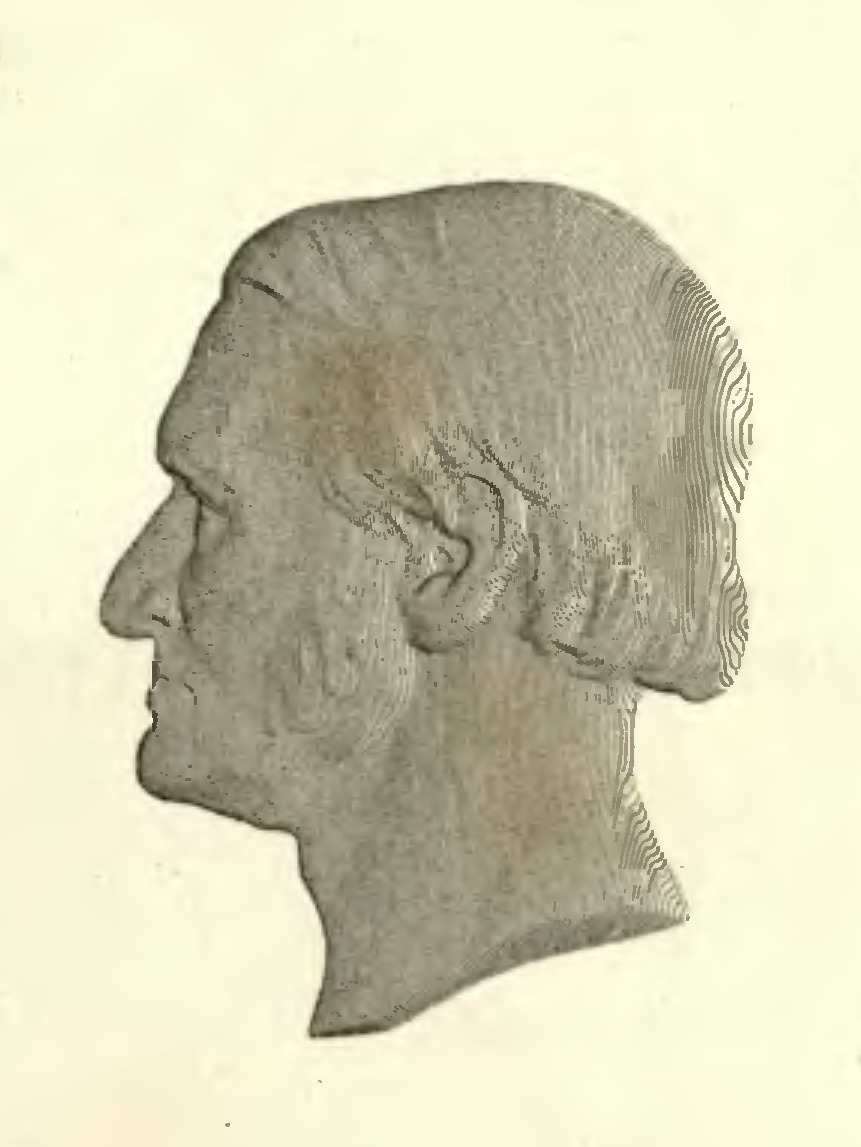
\includegraphics[height=1.93231in]{gauss_title_vignette_1870.jpg}\par
\medskip
EDITED\par
\smallskip
BY THE\par
\smallskip
ROYAL SOCIETY OF SCIENCES\par
\smallskip
AT\par
\smallskip
\textls[180]{GÖTTINGEN.}\par
\medskip
SOLD ON COMMISSION BY B. G. TEUBNER IN LEIPZIG.\par
\medskip
1900.
\end{center}
\clearpage

\SourceLeaf{7}% Otherwise blank verso bears a library ownership stamp, outside the historical body.

% Edition note for the English translation.
\begin{center}\large About this edition\end{center}
\noindent Carl Friedrich Gauss, \emph{Werke}, Volume VIII, Göttingen, 1900.
The Royal Society of Sciences at Göttingen issued the historical edition.
The historical editorial credits include Robert Fricke, Börsch, Krüger, Stäckel, Weingarten, Brendel, and F. Klein.

\noindent This reader contains the historical title matter and portrait and the complete
Arithmetic and Algebra division, with its notes and remarks. This reader includes all of Analysis, including the modular-function and Pentagramma mirificum fragments, and the complete Numerical Calculation and Probability Theory divisions. The complete Foundations of Geometry, Geometria Situs, and Elementary Geometry divisions include the posthumous papers, correspondence, notices, and signed remarks that belong to them. The reader also includes the complete divisions on complex quantities in geometry and the theory of curved surfaces, followed by the historical remarks, corrections, contents, and publisher’s notice. The signed remarks retain their historical authorship. The cropped right-hand portion of historical p. 95 follows the alternative photograph from Kyushu University. The relationship between the photographed copies remains undetermined. References to pages
in the text refer to the historical edition.

\noindent English translation and typesetting by OpenAI GPT-6.1 Sol (Ultra).
Original-language transcription and editable mathematical drawings by OpenAI GPT-6 Astra (Ultra).
The unsigned title vignette is from the \href{https://commons.wikimedia.org/w/index.php?oldid=1179960952}{1870 second printing of \textit{Werke} I}, digitized from the University of California Libraries copy. The same design appears on the \href{https://gdz.sub.uni-goettingen.de/id/PPN236010751}{1900 Göttingen title leaf}. \href{https://creativecommons.org/publicdomain/mark/1.0/}{Public Domain Mark 1.0}.
\clearpage

\SourceLeaf{8}
\thispagestyle{empty}
\vspace*{12em}
\begin{center}
{\Large ARITHMETIC AND ALGEBRA.\par}
\vspace{2em}
SUPPLEMENTS TO VOLUMES I--III.
\end{center}
\clearpage

\SourceLeaf{9}% Blank historical verso, accounted without adding an empty reader page.

\SourceLeaf{10}
\begin{center}
{\Large POSTHUMOUS PAPERS.\par}
\bigskip
[TWO NOTES ON SOLVING THE CONGRUENCE
\[
xx+yy+zz\equiv 0\quad(\mathrm{mod.}\ p).]
\]
\end{center}
\begin{center}[1.]\end{center}
\noindent\hspace*{\parindent}Every representation of a number divisible by the prime number $p$ as a sum of four squares $=aa+bb+cc+dd$ corresponds to a solution of the congruence
\[
xx+yy+zz\equiv 0\quad(\mathrm{mod.}\ p).
\]
\noindent Altogether there are $pp$ such solutions. On removing the one solution $x\equiv0$, $y\equiv0$, $z\equiv0$, the remaining $pp-1$ fall into $p+1$ classes if one counts $x=\xi$, $y=\eta$, $z=\zeta$ and $x\equiv k\xi$, $y\equiv k\eta$, $z\equiv k\zeta$ as belonging to a single class.

For the following are proportional
\[
\begin{array}{c|c|c|c}
x & aa+bb & -ad-bc & bd-ac\\
y & ac+bd & ab-cd & aa+dd\\
z & ad-bc & aa+cc & -ab-cd
\end{array}
\]
\begin{center}[2.]\end{center}
\noindent\hspace*{\parindent}All solutions of the congruence
\[
1+xx+yy\equiv0\quad(\mathrm{mod.}\ p)
\]
\noindent are sought.
\clearpage

\SourceLeaf{11}
They are also the solutions of the congruence
\[
1+(x+iy)^{p+1}\equiv0\quad\text{for}\quad p\equiv3\quad(\mathrm{mod.}\ 4).
\]
\par\indent From one value $x+iy$ one obtains them all by substituting for $u$ all values\\
$0,1,2,3,\, .\, .\, .,p-1$, using the formula\HistoricalNote{[*)]}{[*)}{The following formulas appear alongside this derivation in the manuscript:]
\[
1-xx\equiv yy,\qquad x=1-uy,\qquad 2u-uuy=y
\]
\[
\frac{1-uu}{1+uu}=x,\qquad\frac{2u}{1+uu}=y,
\]
\noindent [which explain the role of the additional factor $\dfrac{uu-1+2iu}{uu+1}$.]}
\[
(x+iy)\left(\frac{uu-1+2iu}{uu+1}\right)\quad\text{or}\quad\frac{(x+iy)(u+i)}{u-i}.
\]
\par\indent For $p\equiv1\ (\mathrm{mod.}\ 4)=aa+bb$, the formula $\dfrac{b}{a}.\dfrac{u+i}{u-i}$ contains all values of $x+iy$, where the only excluded values of $u$ are $\dfrac{a}{b}$ and $\dfrac{b}{a}$.

\clearpage\SourceLeaf{12}
\begin{center}\bfseries [NOTES ON CUBIC AND BIQUADRATIC RESIDUES.]\end{center}
\begin{center}[1.]\par\smallskip A most elegant observation made by induction.\end{center}
\noindent\hspace*{\parindent}2 is a cubic residue or nonresidue of the prime $p$ of the form $3n+1$, according as $p$ can be represented by the form
\[xx+27yy\qquad\text{or}\qquad4xx+2xy+7yy.\]
\par\noindent\hspace*{\parindent}3 is a residue or nonresidue, according as $p$ can be represented by
\[\begin{aligned} &xx+243yy\quad\text{or}\quad4xx+2xy+61yy\\
\text{or}\quad&7xx+6xy+36yy\quad\text{or}\quad9xx+6xy+28yy.\end{aligned}\]
\par\noindent\hspace*{\parindent}5 is a $\left.\begin{array}{l}\text{Residue}\\\text{Nonresidue}\end{array}\right\}$ if $p$ is represented
\begingroup\small
\[\text{by }\left\{\begin{array}{l}(1,0,675),\ (25,0,27),\ (13,1,52),\ (4,1,169)\\
(7,2,97),\ (9,3,76),\ (19,3,36),\ (25,5,28),\ (25,10,31),\ (27,9,28).\end{array}\right.\]
\endgroup
\begin{center}[2.]\end{center}
\noindent\hspace*{\parindent}A criterion for determining whether the number $m$ is a cubic residue of the prime $p$ of the form $3n+1$.

Let
\[4p=aa+27bb\]

\noindent\unskip\SourceLeaf{13}Then the following holds
\begin{center}\footnotesize\setlength{\tabcolsep}{3pt}
\begin{tabular}{@{}rlll@{}}
& &$m\ R\ p$&$m\ N\ p$\\
1)&$m=2$, if&$b$ even&$b$ odd\\
2)&$m=3$&$b$ divis. by 3&\\
3)&\multicolumn{3}{l}{$m={}$ another prime, if $\dfrac{a+b\sqrt{-27}}{a-b\sqrt{-27}}$ a cubic residue of $m$}\\[5pt]
4)&\multicolumn{3}{l}{$m=6$, if either $2b$ or $a+b$ or $a-b$ divis. by 12}\\
5)&\multicolumn{3}{l}{$m=10$, if either $2b$ or $2a$ or $a\pm3b$ or $a\pm9b$ divis. by 20}\\
6)&$m=12$&\multicolumn{2}{l}{$2b,\qquad a+5b,\qquad a-5b$ by 12}\\
7)&$m=15$&\multicolumn{2}{l}{$b,\qquad 3a+5b,\qquad a\pm b,\qquad a\pm2b$ by 15}\\
8)&$m=20$&\multicolumn{2}{l}{$2b,\qquad2a,\qquad a\pm b,\qquad a\pm7b$ by 20}\\
9)&$m=45$&\multicolumn{2}{l}{$b,\qquad3a+5b,\qquad a\pm4b,\qquad a\pm7b$ by 15}\\
10)&$m=14$&\multicolumn{2}{l}{$2b,\qquad2a,\qquad a\pm5b,\qquad a\pm11b$ by 28}\\
11)&$m=28$&\multicolumn{2}{l}{$2b,\qquad2a,\qquad a\pm3b,\qquad a\pm9b$ by 28.}
\end{tabular}\end{center}
\medskip
\par\noindent\hspace*{\parindent}A criterion by which one can determine whether the number $m$ is a biquadratic residue of the prime $p$ of the form $4n+1$.

Let
\[p=aa+4bb\]
\Needspace{17\baselineskip}
\noindent Then $m\ R\ p$ if
\begin{center}\small\setlength{\tabcolsep}{3pt}\begin{tabular}{@{}rlll@{}}
1)&$m=-1$ if&$b$ even&$\pm4$ if $b$ even\\
2)&$m=\pm2$ if&$b$ divis. by 4&$-4$ generally\\
3)&$m=+3$ if&$b$ or $a+3b$ by 6&\\
4)&$m=-3$ if&$b$ by 3&\\
5)&$m=+5$ if&$b$ by 5&\\
6)&$m=-5$ if&$b$ or $a+5b$ by 10&\\
7)&$m=+6$&\multicolumn{2}{l}{$b,\qquad2a+3b,\qquad a\pm b$ by 12}\\
8)&$m=-6$&\multicolumn{2}{l}{$b,\qquad2a+3b,\qquad a\pm5b$ by 12}\\
9)&$m=+7$&\multicolumn{2}{l}{$2a+7b,\qquad b,\qquad a\pm5b$ by 14}
\end{tabular}\end{center}

\SourceLeaf{14}
\begin{center}\small\setlength{\tabcolsep}{3pt}\begin{tabular}{@{}rll@{}}
10)&$m=-7$&$a,\qquad b$ by 7\\
11)&$m=+10$ if&$2a+5b,\qquad b,\qquad a\pm7b$ by 20\\
12)&$m=-10$&$2a+5b,\qquad b,\qquad a\pm3b$ by 20\\
13)&$m=+11$&$2a+11b,\qquad b,\qquad2a\pm3b,\qquad a\pm b$ by 22\\
14)&$m=-11$&$b,\qquad a\pm4b$ by 11.
\end{tabular}\end{center}
\begin{center}[3.]\par\smallskip Cubic residues.\end{center}
\noindent\hspace*{\parindent}$p$ a prime of the form $3m+1$
\[4p=aa+27bb,\]
\par\noindent\hspace*{\parindent}$q$ another prime of the form $3n\pm1$
\[(a+3b\sqrt{-3})^{\frac{q\mp1}{3}}\equiv A\pm B\sqrt{-3}.\]
\par\noindent\hspace*{\parindent}Now there are three cases
\[\begin{array}{rlll}
\text{I.}&B\equiv0\quad\;(\mathrm{mod.}\ q).&\text{Then }q^{\frac{p-1}{3}}\equiv1&\;(\mathrm{mod.}\ p).\\[5pt]
\text{II.}&B\equiv A\quad\;(\mathrm{mod.}\ q).&\text{Then }q^{\frac{p-1}{3}}\equiv-\tfrac12-\tfrac12\dfrac{a}{3b}&\;(\mathrm{mod.}\ p).\\[5pt]
\text{III.}&B\equiv-A\quad\;(\mathrm{mod.}\ q).&\text{Then }q^{\frac{p-1}{3}}\equiv-\tfrac12+\tfrac12\dfrac{a}{3b}&\;(\mathrm{mod.}\ p).
\end{array}\]
\Needspace{9\baselineskip}
\noindent\hspace*{\parindent}First example.\qquad $\begin{array}[t]{ll}p=13,&q=5\\a=5,&b=1\end{array}$
\[(5+3\sqrt{-3})^2=-2+30\sqrt{-3},\quad B\equiv0\ \mathrm{mod.}\ 5\ \text{thus Case I}\]
\[5^4=625\equiv1.\]
\Needspace{9\baselineskip}
\noindent\hspace*{\parindent}Second example.\qquad $\begin{array}[t]{ll}p=19,&q=5\\a=7,&b=1\end{array}$
\[(7+3\sqrt{-3})^2=22+42\sqrt{-3},\quad B\equiv-A\ \text{thus Case III}\]
\[5^6\equiv7\quad\mathrm{mod.}\ 19,\qquad42\equiv-3+7\quad\mathrm{mod.}\ 19.\]

\Needspace{9\baselineskip}
\noindent\SourceLeaf{15}\hspace*{\parindent}Third example.\qquad $\begin{array}[t]{ll}p=7,&q=5\\a=1,&b=1\end{array}$
\[(1+3\sqrt{-3})^2=-26+6\sqrt{-3},\quad B\equiv+A\quad\mathrm{mod.}\ 5\quad\text{Case II}\]
\[5^2\equiv4,\qquad24\equiv-3-1\quad\mathrm{mod.}\ 7.\]
\Needspace{9\baselineskip}
\noindent\hspace*{\parindent}Fourth example.\qquad $p=13,\qquad q=11$
\[(5+3\sqrt{-3})^4=-2696-120\sqrt{-3},\quad A\equiv-1,\quad B=120\equiv-1\]
\[11^4\equiv3,\qquad18+3\equiv-5\quad\mathrm{mod.}\ 13\quad\text{Case II.}\]
\begin{center}Biquadratic residues.\end{center}
\noindent\hspace*{\parindent}$p$ a prime of the form $4n+1$
\[p=aa+4bb,\]
\par\noindent\hspace*{\parindent}$q$ a prime of the form $4n\pm1$
\[(a+2b\sqrt{-1})^{\frac{q\mp1}{4}}=A\pm B\sqrt{-1}.\]
\par\noindent\hspace*{\parindent}Now there are four cases
\[\begin{array}{rll}
\text{I.}&B\equiv0\ (\mathrm{mod.}\ q),&(\pm q)^{\frac{p-1}{4}}\equiv1\ (\mathrm{mod.}\ p).\\[4pt]
\text{II.}&A\equiv0&(\pm q)^{\frac{p-1}{4}}\equiv-1.\\[4pt]
\text{III.}&A\equiv B&(\pm q)^{\frac{p-1}{4}}\equiv-\dfrac{a}{2b}.\\[8pt]
\text{IV.}&A\equiv-B&(\pm q)^{\frac{p-1}{4}}\equiv\dfrac{a}{2b}.
\end{array}\]
\Needspace{9\baselineskip}
\noindent\hspace*{\parindent}First example.\qquad $\begin{array}[t]{ll}p=13,&q=5\\a=3,&b=1\end{array}$
\[(3+2\sqrt{-1})^1=3+2\sqrt{-1},\quad A\equiv-B\quad\text{Case IV}\]
\[5^3\equiv8\equiv\dfrac{3}{2.b}.\]
\Needspace{9\baselineskip}
\noindent\hspace*{\parindent}Second example.\qquad $p=13,\qquad q=7$
\[(3+2\sqrt{-1})^2=5+12\sqrt{-1},\quad A\equiv-B\quad\text{Case IV}\]
\[(-7)^3\equiv8\equiv\dfrac{3}{2.b}.\]

\Needspace{9\baselineskip}
\noindent\SourceLeaf{16}\hspace*{\parindent}Third example.\qquad $p=13,\qquad q=11$
\[(3+2\sqrt{-1})^3=-9+46\sqrt{-1},\quad A\equiv-B\quad\text{Case IV}\]
\[(-11)^3\equiv8\equiv\dfrac{3}{2.b}.\]
\Needspace{9\baselineskip}
\noindent\hspace*{\parindent}Fourth example.\qquad $p=17,\qquad q=11$
\[(1+4\sqrt{-1})^3=-47-52\sqrt{-1},\quad-47=A,\quad+52=B\]
\[A\equiv B\quad\text{Case III}\]
\[(-11)^4\equiv4\equiv-\tfrac14.\]
\begin{center}[4.]\end{center}
\noindent\hspace*{\parindent}Let $p$ be a prime, $n$ a prime $=3m+1$, $R$ a root of the equation $x^3-1=0$, $r$ a root of the equation $r^n-1=0$, and $g$ a primitive root mod. $n$.
\[r+Rr^g+R^2r^{g^2}+R^3r^{g^3}+\ldots+R^{n-2}r^{g^{n-2}}=P,\]
\[P^3=\tfrac12 n(M+N\sqrt{-27}),\]
\noindent where
\[M\equiv1\ (\mathrm{mod.}\ 3),\qquad0\equiv M+3N(g^m-g^{2m})\ (\mathrm{mod.}\ n)\]
\[3k=M+2\]
\[a=\tfrac19(n+1+M)\]
\[b-c=N.\]
\[P^{pp}\equiv r^{pp}+Rr^{ppg}+\ldots\equiv P(R^{\mathrm{ind.}\,p})\]
\begingroup\footnotesize
\[\begin{array}{r@{}l|c}
&1&0\\[3pt]
\{\tfrac12 n(M+N\sqrt{-27})\}^{\frac13(pp-1)}\equiv{}&-\tfrac12+\tfrac12\sqrt{-3}\ (\mathrm{mod.}\ p)&\mathrm{ind.}\ p\equiv1\ (\mathrm{mod.}\ 3)\\[3pt]
&-\tfrac12-\tfrac12\sqrt{-3}&2
\end{array}\]
\endgroup
\[4n=(M+N\sqrt{-27})(M-N\sqrt{-27})\]
\[\dfrac{M}{3N}\equiv g^{2m}-g^m,\qquad-1\equiv g^{2m}+g^m\]
\begingroup\footnotesize
\[\begin{array}{r@{}l|c}
&1&1\\[3pt]
\left\{\dfrac{M-N\sqrt{-27}}{M+N\sqrt{-27}}\right\}^{\frac13(pp-1)}\equiv{}&-\tfrac12+\tfrac12\sqrt{-3}\ (\mathrm{mod.}\ p)&p^{\frac13(n-1)}\equiv-\tfrac12-\tfrac12\dfrac{M}{3N}\ (\mathrm{mod.}\ n)\\[5pt]
&-\tfrac12-\tfrac12\sqrt{-3}&-\tfrac12+\tfrac12\dfrac{M}{3N}
\end{array}\]
\endgroup

\SourceLeaf{17}
\[P^4\equiv PR^{\mathrm{ind.}\,2}\]
\[\tfrac12 M+\tfrac32 N(R-R^2)=\tfrac12(M+3N)+3NR\]
\[\begin{array}{r@{}l|cc}
&1&\tfrac12(M+3N)\ \text{odd}&3N\ \text{even}\\[4pt]
2^{\frac13(n-1)}\equiv{}&-\tfrac12+\tfrac12\dfrac{M}{3N}\ (\mathrm{mod.}\ n)&\text{odd}&\text{odd}\\[5pt]
&-\tfrac12-\tfrac12\dfrac{M}{3N}&\text{even}&\text{odd.}
\end{array}\]
\begin{center}For the cubic residue 3.\end{center}
\[\begin{aligned}
p^3&=m(a-1)+\{m+(a-1)^2+bb+cc\}p\\
&\qquad+\{(a-1)b+bc+ac\}p'\\
&\qquad+\{(a-1)c+ab+bc\}p''\\
&=A+Bp+Cp'+Dp''.
\end{aligned}\]
\noindent Now
\[\begin{array}{rl}1)&aa+bb+cc=ab+ac+bc+a\\2)&a+b+c=m\\3)&3k-2=M\\4)&4a=kk+3NN\\5)&4n=(3k-2)^2+27NN\\6)&4m=3kk-4k+9NN.\end{array}\]
\noindent It follows that
\[\begin{aligned}A&\equiv0\quad\;(\mathrm{mod.}\ 3)\\ B&=\tfrac13(mm-a)-a+m+1\\ C&=\tfrac13(mm-a)-b\\D&=\tfrac13(mm-a)-c\end{aligned}\]
\[\begin{aligned}\tfrac43(mm-a)&\equiv-2k^3+kk-NN\quad\;(\mathrm{mod.}\ 3)\\
&\equiv kk+k-NN\quad\;(\mathrm{mod.}\ 3)\\
&\equiv4a-4m-NN\quad\;(\mathrm{mod.}\ 3).\end{aligned}\]

\noindent\unskip\SourceLeaf{18}Thus
\[\begin{aligned}B&\equiv-NN+1\equiv-(b-c)^2+1\\C&\equiv-NN+b-c\equiv-(b-c)^2+b-c\\D&\equiv-NN-(b-c)\equiv-(b-c)^2-(b-c)\end{aligned}\]
\[\begin{array}{rrrr}
b-c\equiv0&B\equiv1&C\equiv0&D\equiv0\\1&0&0&1\\2&0&1&0.
\end{array}\]
\par\noindent\hspace*{\parindent}Thus, if 3 is a residue modulo $n$, then $N$ is divisible by 3.
\Needspace{10\baselineskip}
\begingroup\small
\begin{center}REMARKS ON THE PRECEDING NOTES CONCERNING CUBIC AND BIQUADRATIC RESIDUES.\end{center}
\noindent\hspace*{\parindent}The note [1] was written by \textsc{Gauss} on the endpaper of the binding of his own copy of the Disquisitiones arithmeticae. The statements under [2] are found in a notebook headed »Uraniae sacrum«, and the two general theorems [3] follow two pages later in the same notebook. The derivations under [4] are taken from several loose slips of paper.

\textsc{Gauss} states at the beginning of his Commentatio prima on the theory of biquadratic residues that in 1805 he began to investigate the theory of cubic and biquadratic residues. In the notebook mentioned above, the derivations given here under [2] and [3] immediately follow notes dated 1804. The »Observatio venustissima« [1], which is less far-reaching than the »Criterien« [2] and [3], can hardly postdate them. We are therefore likely dealing here with \textsc{Gauss}'s earliest investigations and hence with the earliest records of the higher reciprocity laws altogether.

The criteria, like the Observatio, are presumably results of induction. Yet it is very remarkable that the factorization of the quadratic form $aa+27bb$ into its two complex factors, and thus of the number $p$ into its two complex prime divisors, already appears here in the criteria. This had already opened the way for \textsc{Gauss} later to put at least the biquadratic reciprocity law into its simplest form. Incidentally, in certain approaches to proving the general cubic reciprocity law (see the notes immediately following), which in any case date from before 1809, \textsc{Gauss} proceeded, at least at the outset, using rational numbers alone.

The statement made at the beginning of [2] under 3) can be deduced as a special case of the first general theorem under [3]. The latter directly yields the reciprocity law in its most general and simplest form if $p=3m+1$ and $q=3n-1$. For the cubic character of the prime divisor $\pi_1=\dfrac{a+3b\sqrt{-3}}{2}$ with respect to $q$ is given by
\[\left[\frac{\pi_1}{q}\right]\equiv(A-B\sqrt{-3})^{q-1}\quad\;(\mathrm{mod.}\ q)\]

\noindent\unskip\SourceLeaf{19}with the expression congruent to either 1, $\rho$, or $\rho^2$ modulo $q$, where $\rho$ denotes the root of unity
$\dfrac{-1+i\sqrt{3}}{2}$. Now, since in the domain of complex integers formed from $\rho$ the solutions
of the congruence $x^{q-1}\equiv 1\;(\mathrm{mod.}\ q)$ are the $(q-1)$ rational integer residues distinct from 0 modulo $q$,
the division into three cases made by \textsc{Gauss} by means of the congruences $B\equiv 0$, $B\equiv A$, $B\equiv -A\;(\mathrm{mod.}\ q)$ amounts to saying that the cubic character $\left[\dfrac{\pi_1}{q}\right]$ equals 1, $\rho$, or $\rho^2$, respectively. In the other case $q=3n+1$,
the simplest expression of the reciprocity law has yet to be reached here, because the factorization of
$q$ into its prime divisors has yet to be carried out. The connection between \textsc{Gauss}'s theorem and the reciprocity law is as follows.

If the factorizations of the rational primes $p, q$ into their primary prime factors are given by
\[ p=\pi_1.\pi_2,\qquad q=\varkappa_1.\varkappa_2,\qquad \pi_k'=2\pi_k=a\pm 3b\sqrt{-3}, \]
then one must set
\[
\left.\begin{array}{l}
\left[\dfrac{\pi_1'}{\varkappa_1}\right]=\rho^{\varepsilon_1}\equiv {\pi_1'}^{\frac{q-1}{3}}\equiv A+B\rho-B\rho^2 \\[2mm]
\left[\dfrac{\pi_2'}{\varkappa_1}\right]=\rho^{\varepsilon_2}\equiv {\pi_2'}^{\frac{q-1}{3}}\equiv A-B\rho+B\rho^2
\end{array}\right\}(\mathrm{mod.}\ \varkappa_1).
\]

\noindent \textsc{Gauss}'s division into three cases then agrees with the following division
\[
\text{I.}\quad \varepsilon_1\equiv \varepsilon_2 (\mathrm{mod.}\ 3),\qquad \left[\dfrac{\pi_1'}{\varkappa_1}\right]=\left[\dfrac{\pi_2'}{\varkappa_1}\right],
\]
\[
\text{II.}\quad \varepsilon_1\equiv \varepsilon_2+1\;(\mathrm{mod.}\ 3),\qquad \left[\dfrac{\pi_1'}{\varkappa_1}\right]=\rho\left[\dfrac{\pi_2'}{\varkappa_1}\right],
\]
\[
\text{III.}\quad \varepsilon_1\equiv \varepsilon_2-1\;(\mathrm{mod.}\ 3),\qquad \left[\dfrac{\pi_1'}{\varkappa_1}\right]=\rho^2\left[\dfrac{\pi_2'}{\varkappa_1}\right],
\]
where in the last three equations $\pi_k$ can evidently also take the place of $\pi_k'$. Indeed, if e.\,g.
case II holds, then adding and subtracting the above congruences with respect to the modulus $\varkappa_1$ gives
\[
2A\equiv \rho^{\varepsilon_2}(1+\rho)\equiv -\rho^{\varepsilon_2-1},\qquad 2B\equiv -\rho^{\varepsilon_2-1}\qquad\;(\mathrm{mod.}\ \varkappa_1),
\]
so that $(A-B)$ is divisible by $\varkappa_1$ and hence, being a rational number, also by $q$. Thus we do indeed have $B\equiv A\;(\mathrm{mod.}\ q)$. The reciprocity law now gives
\[
\left[\dfrac{\pi_1'}{\varkappa_1}\right]=\left[\dfrac{2}{\varkappa_1}\right].\left[\dfrac{\pi_1}{\varkappa_1}\right]=\left[\dfrac{2}{\varkappa_1}\right].\left[\dfrac{\varkappa_1}{\pi_1}\right],
\]
\[
\left[\dfrac{\pi_2'}{\varkappa_1}\right]=\left[\dfrac{2}{\varkappa_1}\right].\left[\dfrac{\pi_2}{\varkappa_1}\right]=\left[\dfrac{2}{\varkappa_1}\right].\left[\dfrac{\varkappa_1}{\pi_2}\right],
\]
so that in case II we further obtain
\[
\left[\dfrac{\varkappa_1}{\pi_1}\right]=\rho\left[\dfrac{\varkappa_1}{\pi_2}\right]=\rho\left[\dfrac{\varkappa_2}{\pi_1}\right]^2,\qquad
\left[\dfrac{\varkappa_1}{\pi_1}\right].\left[\dfrac{\varkappa_2}{\pi_1}\right]=\left[\dfrac{q}{\pi_1}\right]=\rho,
\]
\[
\left[\dfrac{q}{\pi_1}\right]\equiv q^{\frac{p-1}{3}}\equiv -\tfrac12+\tfrac12\sqrt{-3}\equiv -\tfrac12-\tfrac12\dfrac{a}{3b}\qquad\;(\mathrm{mod.}\ \pi_1).
\]
But if the rational number satisfies $q^{\frac{p-1}{3}}+\tfrac12+\tfrac12\dfrac{a}{3b}\equiv 0 \mathrm{mod.}\ \pi_1$, then it is also divisible by $\pi_2$ and hence by $p$.
This gives the congruence stated under II by \textsc{Gauss} with respect to the modulus $p$.
Cases I and III are handled in the same way.

\SourceLeaf{20}

Reversing the preceding derivation shows that from \textsc{Gauss}'s statements, in the
case $q=3n+1$, one can first infer the proportion
\[
\left[\dfrac{\varkappa_1}{\pi_1}\right]:\left[\dfrac{\pi_1}{\varkappa_1}\right]=\left[\dfrac{\varkappa_1}{\pi_2}\right]:\left[\dfrac{\pi_2}{\varkappa_1}\right]
\]
Applying once more the law expressed in this proportion, one finds
\[
\dfrac{\left[\dfrac{\varkappa_1}{\pi_1}\right]}{\left[\dfrac{\pi_1}{\varkappa_1}\right]}=\dfrac{\left[\dfrac{\varkappa_2}{\pi_1}\right]}{\left[\dfrac{\pi_1}{\varkappa_2}\right]}=\dfrac{\left[\dfrac{\varkappa_1}{\pi_2}\right]^2}{\left[\dfrac{\pi_2}{\varkappa_1}\right]^2}
\quad\text{and hence}\quad
\dfrac{\left[\dfrac{\varkappa_1}{\pi_2}\right]}{\left[\dfrac{\pi_2}{\varkappa_1}\right]}=\dfrac{\left[\dfrac{\varkappa_1}{\pi_2}\right]^3}{\left[\dfrac{\pi_2}{\varkappa_1}\right]^2}.
\]
Since $\left[\dfrac{\varkappa_1}{\pi_2}\right]=\left[\dfrac{\pi_2}{\varkappa_1}\right]$ follows from this, the general reciprocity law in its simplest form is, for $q=3n+1$ as well, implicitly contained in \textsc{Gauss}'s statements.

The notes in which \textsc{Gauss} proved his cubic reciprocity theorems are collected under [4]. Since these notes come from several undated loose slips, the date of the proofs in question cannot be determined with certainty. It is
likely, however, that the derivations were carried out soon after he obtained the »Observatio« and the »Criterien«,
for their line of reasoning is very closely connected with the first statements under [2]
and, moreover, with Art. 358 of the Disquisitiones arithmeticae. On the other hand, \textsc{Gauss}, by his own
account\HistoricalNote{\textsuperscript{*)}}{*)}{See Art. 33 of the treatise »Summatio quarumdam serierum singularium«, presented to the Göttingen Society on 24 August 1808.}, was in any case in possession, before the middle of 1808, of the sixth proof of the quadratic
reciprocity law. That proof is the one most closely related to the proofs under consideration here.

\textsc{Gauss}'s proof of the cubic reciprocity law is based on cyclotomy. The
individual formulas under [4] can either be taken directly from Art. 358 of the Disquisitiones arithmeticae or at least be derived with very little effort from the developments given there.
The congruence
\[
P^{pp}\equiv r^{pp}+Rr^{ppg}+\ldots\equiv P(R^{\mathrm{ind.}\,p})
\]
is modulo $p$ and arises from the fact that all polynomial coefficients of the power $pp$ other than 1 are divisible by $p$. The distinction between the cases
\[
\left\{\dfrac{M-N\sqrt{-27}}{M+N\sqrt{-27}}\right\}^{\frac13(pp-1)}\equiv 1,\quad -\tfrac12+\tfrac12\sqrt{-3},\quad -\tfrac12-\tfrac12\sqrt{-3}\qquad\;(\mathrm{mod.}\ p)
\]
corresponds exactly, for both $p=3m-1$ and $p=3m+1$, to the distinction made above under I, II and III,
namely $B\equiv 0\;(\mathrm{mod.}\ q)$, etc. The correspondence between those three congruences and the following
\[
p^{\frac13(n-1)}\equiv 1,\quad -\tfrac12-\tfrac12\dfrac{M}{3N},\quad -\tfrac12+\tfrac12\dfrac{M}{3N}\qquad\;(\mathrm{mod.}\ n),
\]
as developed in [4], therefore already contains a complete proof of \textsc{Gauss}'s statements
and thus implicitly of the general cubic reciprocity law.

The further discussion under [4] concerns the criteria for 2 and 3 to be cubic residues.
As for 3 as a cubic residue, it suffices to note that (using the notation in [4])
$p^3\equiv p, p'$ or $p''\;(\mathrm{mod.}\ 3)$ holds according to whether ind.\,$3\equiv 0, 1$ or $2\;(\mathrm{mod.}\ 3)$ holds. The condition
$N\equiv 0\;(\mathrm{mod.}\ 3)$ for 3 to be a cubic residue modulo $n$ then follows directly from the concluding statements of [4].


\SourceLeaf{21}

The Observatio can easily be derived from the Criterien. For\,example, for 3 to be a cubic residue,
the condition $N\equiv 0\;(\mathrm{mod.}\ 3)$ was just obtained and is likewise stated under [2]. If $M$ and $N$
are even, put
\[ M=2x,\qquad N=6y, \]
so that $4n=M^2+27N^2$ implies that $n$ is representable by the quadratic form of determinant $-243$
\[ n=x^2+243y^2 \]
with integers $x, y$. Conversely, the possibility of such a representation of $n$
implies the validity of the congruence $N\equiv 0\;(\mathrm{mod.}\ 3)$. If $M$ and $N$ are odd, choose the appropriate sign and put
\[ M\pm\dfrac{N}{3}=4x,\qquad \mp\dfrac{N}{3}=y, \]
which gives the representation
\[ n=4x^2+2xy+61y^2. \]
Conversely, this formula would imply $N\equiv 0\;(\mathrm{mod.}\ 3)$, so that 3 is a cubic residue
modulo $n$ if and only if $n$ is representable by one of the forms $(1,0,243)$, $(4,1,61)$.

Mr. R. \textsc{Dedekind}, to whom I owe several very helpful conversations on the subjects in question,
drew my attention to the fact that, in the case where
3 is a cubic nonresidue modulo $n$, \textsc{Gauss}'s statements are not quite complete. There are altogether nine classes of primitive forms of the first kind of determinant $D=-243$, whose reduced forms are the following
\[ (1,0,243),\quad (4,\pm1,61),\quad (13,\pm2,19),\quad (7,\pm3,36),\quad (9,\pm3,28). \]
In [1] the forms $(13,\pm2,19)$ are missing. The theorem must therefore state that 3 is a cubic
nonresidue modulo $n$ if and only if $n$ admits a representation in one of the forms
\[ n=13xx+4xy+19yy, \]
\[ n=7xx+6xy+36yy, \]
\[ n=9xx+6xy+28yy. \]
These representations can always be obtained by choosing the appropriate sign in the following transformations
\[ \text{I. If } M\equiv N\equiv 1\;(\mathrm{mod.}\ 2),\quad M\pm 7N\equiv 0\;(\mathrm{mod.}\ 12), \]
\[ M=5x+7y,\qquad \pm N=x-y. \]
\[ \text{II. If } M\equiv N\equiv 1\;(\mathrm{mod.}\ 2),\quad M\pm 7N\equiv 6\;(\mathrm{mod.}\ 12), \]
\[ M=x+6y,\qquad \mp N=x. \]
\[ \text{III. If } M\equiv N\equiv 0\;(\mathrm{mod.}\ 2),\quad M\pm N\equiv 0\;(\mathrm{mod.}\ 3), \]
\[ M=6x+2y,\qquad \mp N=2y. \]
\par\noindent\hspace*{\parindent}The statements about the number 5 given under 1 follow in a similar way from the residue criterion
$MN\equiv 0\;(\mathrm{mod.}\ 5)$.

It should also be noted that the original of note [1] contains a table extending to 223 of the primes $p=3n+1$ modulo which the numbers 2, 3, 5, 7 are cubic residues.

\hfill \textsc{Fricke.}

\endgroup

\clearpage\SourceLeaf{22}
\begin{center}
\bfseries ON THE THEORY OF CUBIC RESIDUES.
\end{center}



\begin{center}
[1.]
\end{center}

\[ p=mm+3nn \text{ a prime number.} \]

\noindent\hspace*{\parindent}For any integer indivisible by $p$, denoted by $x$, let
\[
\left[\dfrac{2mx}{p}\right]=\alpha,\qquad \left[\dfrac{(3n-m)x}{p}\right]=\beta,\qquad \left[\dfrac{(-3n-m)x}{p}\right]=\gamma.
\]
\noindent As is readily seen, this makes
\[
\dfrac{2mx}{p}-\alpha+\dfrac{(3n-m)x}{p}-\beta+\dfrac{(-3n-m)x}{p}-\gamma
\]
the sum of three proper fractions, so it must lie strictly between the limits
0 and 3. Since this same sum is evidently $=-\alpha-\beta-\gamma$, and hence an integer,
its only possible values are $+1$ and $+2$.
Thus either
\[ \alpha+\beta+\gamma=-1\quad\text{or}\quad \alpha+\beta+\gamma=-2. \]

\noindent It follows further that the three quantities $\alpha, \beta, \gamma$ cannot all be congruent
to one another modulo 3. Among the differences $\alpha-\beta$, $\beta-\gamma$,
$\gamma-\alpha$ there will therefore be at least one (and for that very reason at least one more,

\SourceLeaf{23}
since the sum of them all is $=0$) that is not $\equiv 0$. Nor can the quantities
$\alpha, \beta, \gamma$ all be incongruent to one another, for then they would be congruent,
in some order, to the numbers $0, 1, 2$, so their sum would be divisible by
$3$. Among the differences $\alpha-\beta$,
$\beta-\gamma$, $\gamma-\alpha$ there is therefore exactly one that is
$\equiv 0$. Thus there are three mutually exclusive cases:

\[
\text{I.} \quad \text{If } \beta \equiv \gamma \quad(\mathrm{mod.}\ 3)
\]
\[
\text{II.} \quad \text{If } \gamma \equiv \alpha \quad(\mathrm{mod.}\ 3)
\]
\[
\text{III.} \quad \text{If } \alpha \equiv \beta \quad(\mathrm{mod.}\ 3).
\]

Which of these three cases occurs depends on $x$. Accordingly, we divide
all numbers indivisible by $p$ into three classes. We put the numbers for
which the first case occurs into the first class, those for which the second
occurs into the second, and those for which the third occurs into the third.

\textls[100]{First Theorem:} All numbers congruent modulo $p$ belong to
one and the same class.

\textls[100]{Second Theorem:} Numbers of equal magnitude and opposite signs
belong to the same class.

It is clear from this that one need only classify the numbers $1, 2, 3, \ldots,
\frac{1}{2}(p-1)$
to be able to classify all the others at once.

\textls[100]{Third Theorem:} The numbers $(3n-m)x$ and $2mx$ belong to two
consecutive classes.

\textls[100]{Fourth Theorem:} Thus if $\dfrac{2n-m}{3m} \equiv f$, so that

\[
1+f+ff \equiv 0 \quad(\mathrm{mod.}\ p), \qquad 1 \equiv f^3 \quad(\mathrm{mod.}\ p),
\]
\noindent then $x$ and the residues of $fx$ and $ffx$ belong to
three consecutive classes in reverse order.


\clearpage\SourceLeaf{24}
\begin{center}\textls[100]{Examples of the classification.}\end{center}


\begingroup\small
\[p = 7 = 4+3, \qquad 4,\quad 1,\quad -5\]
\begin{center}\begin{tabular}{@{}rl@{}}
I. & 3.\ 4.\\
II. & 2.\ 5.\\
III. & 1.\ 6.\end{tabular}\end{center}
\[p = 13 = 1+12, \qquad 2,\quad 5,\quad -7\]
\begin{center}\begin{tabular}{@{}rl@{}}
I. & 3.\ 6.\ 7.\ 10.\\
II. & 4.\ 5.\ 8.\ 9.\\
III. & 1.\ 2.\ 11.\ 12.\end{tabular}\end{center}
\[p = 19 = 16+3, \qquad 8,\quad -1,\quad -7\]
\begin{center}\begin{tabular}{@{}rl@{}}
I. & 1.\ 2.\ 9.\ 10.\ 17.\ 18.\\
II. & 3.\ 4.\ 8.\ 11.\ 15.\ 16.\\
III. & 5.\ 6.\ 7.\ 12.\ 13.\ 14.\end{tabular}\end{center}
\[p = 31 = 4+27, \qquad 4,\quad 7,\quad -11\]
\begin{center}\begin{tabular}{@{}rl@{}}
I. & 5.\ 9.\ 10.\ 11.\ 15.\ 16.\ 20.\ 21.\ 22.\ 26.\\
II. & 6.\ 7.\ 12.\ 13.\ 14.\ 17.\ 18.\ 19.\ 24.\ 25.\\
III. & 1.\ 2.\ 3.\ 4.\ 8.\ 23.\ 27.\ 28.\ 29.\ 30.\end{tabular}\end{center}
\[p = 37 = 25+12, \qquad 10,\quad 1,\quad -11\]
\begin{center}\begin{tabular}{@{}rl@{}}
I. & 7.\ 8.\ 9,\ 10.\ 17.\ 18.\ 19.\ 20.\ 27.\ 28.\ 29.\ 30.\\
II. & 4.\ 5.\ 6.\ 11.\ 15.\ 16.\ 21.\ 22.\ 26.\ 31.\ 32.\ 33.\\
III. & 1.\ 2.\ 3.\ 12.\ 13.\ 14.\ 23.\ 24.\ 25.\ 34.\ 35.\ 36.\end{tabular}\end{center}
\[p = 43 = 16+27, \qquad 8,\quad 5,\quad -13\]
\begin{center}\begin{tabular}{@{}rl@{}}
I. & 7.\ 8.\ 14.\ 15.\ 16.\ 20.\ 21.\ 22.\ 23.\ 27.\ 28.\ 29.\ 35.\ 36.\\
II. & 6.\ 11.\ 12.\ 13.\ 17.\ 18.\ 19.\ 24.\ 25.\ 26.\ 30.\ 31.\ 32.\ 37.\\
III. & 1.\ 2.\ 3.\ 4.\ 5.\ 9.\ 10.\ 33.\ 34.\ 38.\ 39.\ 40.\ 41.\ 42.\end{tabular}\end{center}
\begin{center}
\begin{tabular}[t]{c|c|c}
\multicolumn{3}{c}{$7,\quad2-\rho$}\\\hline
$1$&$-\rho\rho$&$\rho$\\
$-1$&$\rho\rho$&$-\rho$
\end{tabular}\qquad
\begin{tabular}[t]{c|c|c}
\multicolumn{3}{c}{$13,\quad3-\rho$}\\\hline
$1$&$1-\rho$&$-\rho\rho$\\
$1-\rho\rho$&$\rho$&$\rho-\rho\rho$\\
$-1$&$-1+\rho$&$\rho\rho$\\
$-1+\rho\rho$&$-\rho$&$-\rho+\rho\rho$
\end{tabular}
\end{center}\endgroup

\clearpage\SourceLeaf{25}
\begin{center}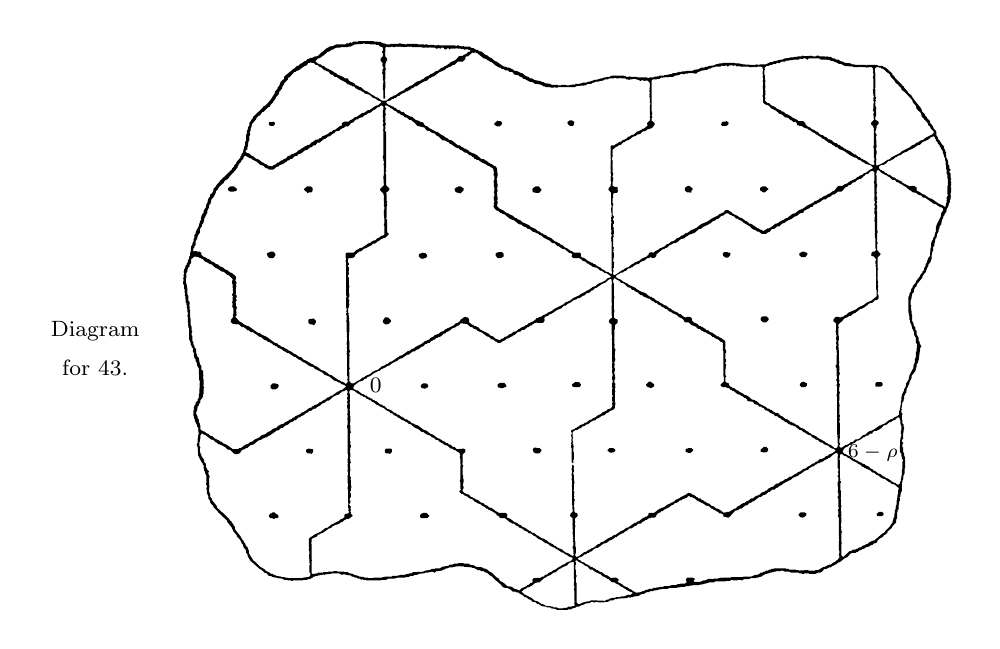
\begin{tikzpicture}[x=.195pt,y=-.195pt]
\path[use as bounding box] (0,0) rectangle (1750,1100);
\path[fill=black,even odd rule] (414,171) -- (413,174) -- (411,176) -- (411,181) -- (408,185) -- (408,188) -- (406,192) -- (406,197) -- (405,198) -- (405,209) -- (403,212) -- (403,218) -- (401,221) -- (401,224) -- (400,225) -- (399,231) -- (396,235) -- (396,237) -- (394,239) -- (394,241) -- (387,249) -- (386,252) -- (383,255) -- (382,258) -- (379,261) -- (379,262) -- (376,265) -- (375,265) -- (374,267) -- (355,285) -- (355,286) -- (351,290) -- (348,295) -- (344,299) -- (344,302) -- (342,306) -- (340,308) -- (339,308) -- (338,310) -- (338,313) -- (336,315) -- (334,319) -- (333,325) -- (331,327) -- (331,329) -- (330,330) -- (330,334) -- (328,336) -- (326,340) -- (326,343) -- (324,345) -- (322,349) -- (322,351) -- (321,352) -- (321,354) -- (322,355) -- (319,359) -- (319,362) -- (318,363) -- (317,368) -- (311,379) -- (311,382) -- (309,384) -- (309,389) -- (308,390) -- (307,397) -- (305,400) -- (305,403) -- (303,405) -- (302,416) -- (301,417) -- (301,422) -- (299,425) -- (299,429) -- (297,431) -- (297,434) -- (295,437) -- (295,439) -- (292,442) -- (292,445) -- (290,448) -- (290,451) -- (289,452) -- (290,456) -- (289,457) -- (289,464) -- (288,465) -- (289,467) -- (289,469) -- (288,470) -- (288,474) -- (290,478) -- (290,484) -- (291,485) -- (291,491) -- (292,492) -- (291,496) -- (292,497) -- (293,509) -- (294,510) -- (294,513) -- (295,514) -- (295,520) -- (296,521) -- (296,527) -- (297,528) -- (297,532) -- (296,533) -- (296,535) -- (297,536) -- (297,547) -- (298,548) -- (297,551) -- (298,552) -- (298,556) -- (299,557) -- (299,578) -- (301,580) -- (301,582) -- (302,583) -- (302,587) -- (304,590) -- (304,592) -- (307,595) -- (306,599) -- (308,603) -- (308,609) -- (309,610) -- (309,612) -- (311,614) -- (311,618) -- (313,620) -- (314,626) -- (317,631) -- (318,654) -- (319,655) -- (318,678) -- (317,679) -- (317,686) -- (315,689) -- (315,691) -- (311,695) -- (311,698) -- (309,700) -- (309,702) -- (308,703) -- (308,709) -- (307,710) -- (307,713) -- (308,714) -- (307,715) -- (307,719) -- (308,720) -- (308,723) -- (310,726) -- (310,729) -- (314,737) -- (314,739) -- (317,743) -- (316,744) -- (317,754) -- (316,755) -- (316,760) -- (315,761) -- (315,763) -- (316,764) -- (315,765) -- (315,769) -- (313,773) -- (315,777) -- (316,793) -- (322,805) -- (324,807) -- (324,809) -- (326,811) -- (326,817) -- (327,818) -- (327,821) -- (329,823) -- (329,826) -- (331,830) -- (331,844) -- (330,846) -- (332,848) -- (332,852) -- (331,853) -- (331,855) -- (332,856) -- (332,862) -- (335,869) -- (335,873) -- (337,875) -- (339,881) -- (344,886) -- (344,888) -- (352,896) -- (352,897) -- (369,913) -- (370,916) -- (378,926) -- (381,933) -- (387,940) -- (388,943) -- (393,948) -- (396,953) -- (396,955) -- (399,958) -- (400,963) -- (404,967) -- (405,973) -- (407,975) -- (408,980) -- (413,988) -- (430,1003) -- (434,1005) -- (439,1010) -- (443,1011) -- (446,1015) -- (448,1016) -- (451,1016) -- (454,1018) -- (457,1018) -- (458,1019) -- (462,1019) -- (463,1020) -- (472,1021) -- (475,1023) -- (481,1023) -- (482,1024) -- (488,1024) -- (489,1025) -- (491,1025) -- (492,1024) -- (510,1024) -- (511,1023) -- (518,1023) -- (519,1022) -- (522,1022) -- (528,1019) -- (530,1017) -- (532,1017) -- (533,1016) -- (537,1016) -- (538,1015) -- (541,1015) -- (542,1014) -- (546,1014) -- (547,1013) -- (550,1014) -- (551,1013) -- (562,1012) -- (563,1011) -- (577,1011) -- (582,1014) -- (584,1013) -- (589,1013) -- (590,1014) -- (599,1015) -- (601,1017) -- (603,1017) -- (607,1019) -- (610,1019) -- (612,1021) -- (616,1021) -- (618,1023) -- (621,1022) -- (622,1023) -- (626,1023) -- (627,1024) -- (655,1024) -- (656,1023) -- (664,1023) -- (668,1021) -- (680,1021) -- (681,1020) -- (684,1020) -- (685,1019) -- (699,1019) -- (700,1018) -- (705,1018) -- (709,1016) -- (714,1016) -- (717,1014) -- (721,1014) -- (725,1012) -- (735,1011) -- (736,1010) -- (742,1010) -- (743,1009) -- (747,1009) -- (748,1008) -- (750,1008) -- (754,1010) -- (757,1007) -- (768,1006) -- (770,1004) -- (772,1004) -- (775,1002) -- (778,1002) -- (781,1000) -- (788,1000) -- (789,999) -- (792,999) -- (793,998) -- (798,998) -- (800,997) -- (801,998) -- (808,998) -- (809,999) -- (823,1000) -- (824,1001) -- (827,1001) -- (834,1005) -- (837,1005) -- (841,1007) -- (845,1007) -- (847,1009) -- (851,1010) -- (858,1016) -- (859,1016) -- (868,1025) -- (869,1025) -- (874,1030) -- (875,1030) -- (881,1037) -- (883,1037) -- (884,1038) -- (889,1038) -- (896,1042) -- (899,1045) -- (904,1045) -- (905,1046) -- (910,1047) -- (912,1049) -- (918,1052) -- (921,1055) -- (923,1055) -- (930,1060) -- (932,1060) -- (936,1064) -- (940,1064) -- (945,1068) -- (947,1068) -- (953,1072) -- (961,1073) -- (962,1074) -- (968,1074) -- (970,1076) -- (978,1077) -- (981,1079) -- (1000,1079) -- (1001,1078) -- (1007,1078) -- (1009,1076) -- (1014,1075) -- (1017,1073) -- (1021,1073) -- (1026,1070) -- (1028,1070) -- (1034,1067) -- (1042,1066) -- (1044,1064) -- (1047,1064) -- (1048,1065) -- (1051,1065) -- (1052,1064) -- (1056,1064) -- (1057,1065) -- (1068,1065) -- (1069,1064) -- (1075,1064) -- (1080,1061) -- (1085,1061) -- (1088,1059) -- (1092,1059) -- (1093,1058) -- (1110,1057) -- (1114,1055) -- (1115,1056) -- (1117,1056) -- (1118,1055) -- (1122,1055) -- (1123,1054) -- (1132,1053) -- (1136,1050) -- (1142,1049) -- (1147,1046) -- (1151,1046) -- (1154,1044) -- (1159,1044) -- (1160,1043) -- (1168,1042) -- (1169,1041) -- (1174,1041) -- (1175,1040) -- (1186,1040) -- (1189,1038) -- (1191,1038) -- (1192,1039) -- (1194,1038) -- (1203,1038) -- (1204,1037) -- (1209,1037) -- (1210,1036) -- (1218,1036) -- (1219,1035) -- (1225,1035) -- (1226,1034) -- (1231,1034) -- (1232,1033) -- (1244,1033) -- (1245,1032) -- (1249,1032) -- (1250,1031) -- (1253,1031) -- (1254,1030) -- (1257,1030) -- (1258,1029) -- (1261,1029) -- (1262,1028) -- (1271,1028) -- (1274,1026) -- (1293,1026) -- (1294,1025) -- (1301,1025) -- (1305,1023) -- (1307,1024) -- (1315,1024) -- (1316,1023) -- (1321,1023) -- (1322,1024) -- (1324,1024) -- (1327,1022) -- (1336,1022) -- (1340,1020) -- (1349,1020) -- (1350,1019) -- (1354,1019) -- (1355,1018) -- (1360,1017) -- (1362,1015) -- (1365,1014) -- (1366,1012) -- (1370,1012) -- (1371,1011) -- (1374,1011) -- (1375,1010) -- (1378,1010) -- (1379,1009) -- (1382,1009) -- (1383,1008) -- (1386,1008) -- (1387,1007) -- (1395,1007) -- (1396,1006) -- (1399,1006) -- (1403,1008) -- (1411,1008) -- (1415,1010) -- (1429,1010) -- (1430,1011) -- (1434,1011) -- (1435,1012) -- (1438,1012) -- (1439,1011) -- (1447,1011) -- (1448,1012) -- (1460,1012) -- (1464,1010) -- (1468,1010) -- (1472,1008) -- (1475,1004) -- (1477,1003) -- (1480,1003) -- (1485,1000) -- (1488,1000) -- (1492,997) -- (1494,997) -- (1496,995) -- (1499,994) -- (1502,991) -- (1504,991) -- (1514,983) -- (1519,981) -- (1524,975) -- (1528,973) -- (1534,973) -- (1535,972) -- (1537,972) -- (1542,968) -- (1544,968) -- (1547,966) -- (1549,966) -- (1553,963) -- (1560,961) -- (1562,959) -- (1566,958) -- (1567,956) -- (1572,955) -- (1574,953) -- (1575,950) -- (1579,946) -- (1581,946) -- (1583,944) -- (1584,944) -- (1587,940) -- (1588,940) -- (1593,936) -- (1593,934) -- (1601,927) -- (1603,923) -- (1609,917) -- (1609,912) -- (1611,909) -- (1611,898) -- (1612,897) -- (1612,894) -- (1614,892) -- (1614,884) -- (1615,883) -- (1615,878) -- (1616,877) -- (1616,872) -- (1615,871) -- (1617,869) -- (1618,861) -- (1620,859) -- (1620,843) -- (1621,842) -- (1621,839) -- (1622,838) -- (1623,829) -- (1625,826) -- (1625,817) -- (1626,816) -- (1626,810) -- (1625,809) -- (1626,808) -- (1626,801) -- (1625,800) -- (1626,797) -- (1624,793) -- (1624,789) -- (1622,786) -- (1622,778) -- (1621,777) -- (1621,774) -- (1620,773) -- (1622,771) -- (1622,769) -- (1620,767) -- (1620,764) -- (1622,762) -- (1622,751) -- (1623,750) -- (1623,745) -- (1624,744) -- (1624,741) -- (1623,740) -- (1623,735) -- (1621,733) -- (1621,727) -- (1620,726) -- (1620,718) -- (1621,717) -- (1621,715) -- (1619,713) -- (1619,709) -- (1620,708) -- (1619,706) -- (1619,704) -- (1620,703) -- (1620,697) -- (1621,696) -- (1621,694) -- (1623,692) -- (1623,689) -- (1624,688) -- (1624,682) -- (1626,680) -- (1626,678) -- (1628,676) -- (1629,668) -- (1631,666) -- (1632,662) -- (1634,660) -- (1634,657) -- (1638,649) -- (1638,645) -- (1645,636) -- (1646,630) -- (1647,629) -- (1647,624) -- (1650,620) -- (1650,617) -- (1651,616) -- (1654,593) -- (1656,591) -- (1653,585) -- (1653,582) -- (1651,580) -- (1651,575) -- (1647,568) -- (1647,562) -- (1645,560) -- (1645,556) -- (1644,554) -- (1642,553) -- (1641,547) -- (1639,544) -- (1639,541) -- (1638,540) -- (1639,539) -- (1639,532) -- (1638,531) -- (1638,525) -- (1637,524) -- (1637,520) -- (1636,519) -- (1637,517) -- (1637,515) -- (1636,514) -- (1636,505) -- (1637,504) -- (1639,493) -- (1642,490) -- (1642,486) -- (1644,482) -- (1647,479) -- (1648,475) -- (1658,463) -- (1658,461) -- (1661,456) -- (1665,452) -- (1665,449) -- (1666,448) -- (1666,446) -- (1669,442) -- (1669,439) -- (1673,434) -- (1674,430) -- (1675,429) -- (1675,421) -- (1676,420) -- (1676,416) -- (1678,412) -- (1678,406) -- (1680,404) -- (1680,399) -- (1681,398) -- (1682,391) -- (1684,389) -- (1685,383) -- (1688,377) -- (1688,374) -- (1689,373) -- (1690,368) -- (1693,364) -- (1694,356) -- (1696,354) -- (1697,349) -- (1699,347) -- (1699,345) -- (1701,343) -- (1703,339) -- (1703,336) -- (1706,331) -- (1707,326) -- (1709,323) -- (1709,319) -- (1710,318) -- (1710,314) -- (1711,313) -- (1710,311) -- (1710,306) -- (1711,305) -- (1711,296) -- (1710,295) -- (1711,293) -- (1711,285) -- (1710,284) -- (1710,282) -- (1711,281) -- (1711,279) -- (1710,278) -- (1710,270) -- (1708,268) -- (1708,266) -- (1710,264) -- (1710,263) -- (1708,261) -- (1708,256) -- (1706,254) -- (1705,246) -- (1702,240) -- (1702,235) -- (1701,234) -- (1702,231) -- (1700,229) -- (1700,226) -- (1698,224) -- (1698,221) -- (1697,219) -- (1694,216) -- (1689,208) -- (1687,207) -- (1687,204) -- (1684,200) -- (1684,194) -- (1682,190) -- (1679,187) -- (1677,182) -- (1672,176) -- (1672,173) -- (1666,167) -- (1666,166) -- (1663,163) -- (1662,160) -- (1657,155) -- (1657,153) -- (1655,149) -- (1640,130) -- (1638,126) -- (1631,120) -- (1631,119) -- (1624,111) -- (1624,110) -- (1622,108) -- (1621,108) -- (1620,106) -- (1608,94) -- (1605,89) -- (1603,88) -- (1602,85) -- (1590,74) -- (1586,73) -- (1584,71) -- (1577,71) -- (1573,69) -- (1556,69) -- (1555,70) -- (1553,69) -- (1533,69) -- (1532,68) -- (1528,68) -- (1524,66) -- (1514,65) -- (1511,63) -- (1506,62) -- (1502,59) -- (1498,59) -- (1495,57) -- (1492,57) -- (1488,54) -- (1483,54) -- (1482,53) -- (1478,54) -- (1477,53) -- (1467,53) -- (1466,52) -- (1462,52) -- (1461,53) -- (1454,53) -- (1453,52) -- (1438,53) -- (1437,52) -- (1435,52) -- (1434,53) -- (1427,53) -- (1426,54) -- (1420,54) -- (1419,55) -- (1413,55) -- (1412,56) -- (1403,57) -- (1399,59) -- (1391,60) -- (1390,61) -- (1383,62) -- (1379,64) -- (1376,64) -- (1368,68) -- (1357,68) -- (1356,69) -- (1350,68) -- (1349,69) -- (1345,69) -- (1344,70) -- (1343,69) -- (1325,68) -- (1324,67) -- (1320,67) -- (1319,66) -- (1311,66) -- (1310,65) -- (1288,65) -- (1287,66) -- (1282,66) -- (1281,67) -- (1278,67) -- (1271,70) -- (1262,71) -- (1261,72) -- (1255,73) -- (1254,74) -- (1248,74) -- (1243,77) -- (1236,78) -- (1232,80) -- (1220,80) -- (1219,81) -- (1213,81) -- (1212,82) -- (1207,82) -- (1206,83) -- (1203,83) -- (1202,84) -- (1196,84) -- (1193,86) -- (1190,86) -- (1189,87) -- (1185,87) -- (1184,88) -- (1180,88) -- (1179,89) -- (1170,89) -- (1169,90) -- (1161,91) -- (1160,92) -- (1153,92) -- (1152,93) -- (1148,93) -- (1147,92) -- (1130,92) -- (1129,91) -- (1117,91) -- (1116,90) -- (1114,91) -- (1109,91) -- (1108,90) -- (1105,90) -- (1104,89) -- (1082,89) -- (1078,91) -- (1073,91) -- (1072,92) -- (1069,92) -- (1065,94) -- (1062,94) -- (1061,95) -- (1058,95) -- (1057,96) -- (1049,97) -- (1048,98) -- (1046,98) -- (1042,100) -- (1039,100) -- (1035,102) -- (1028,102) -- (1027,103) -- (1024,103) -- (1023,104) -- (1016,104) -- (1013,106) -- (1010,105) -- (1009,106) -- (1005,106) -- (1004,107) -- (998,107) -- (997,106) -- (989,106) -- (988,107) -- (983,107) -- (982,106) -- (971,106) -- (968,104) -- (959,103) -- (956,101) -- (954,101) -- (950,99) -- (939,97) -- (935,94) -- (931,94) -- (929,92) -- (922,89) -- (916,84) -- (914,84) -- (906,80) -- (902,80) -- (900,78) -- (892,74) -- (889,74) -- (885,72) -- (882,72) -- (869,63) -- (866,62) -- (859,56) -- (856,55) -- (851,51) -- (849,51) -- (842,45) -- (840,44) -- (837,44) -- (834,41) -- (831,41) -- (826,38) -- (823,38) -- (819,35) -- (809,35) -- (808,34) -- (804,35) -- (803,34) -- (800,34) -- (799,33) -- (796,33) -- (795,34) -- (793,34) -- (792,33) -- (763,33) -- (762,32) -- (760,32) -- (759,33) -- (754,33) -- (753,32) -- (741,32) -- (740,31) -- (737,31) -- (736,32) -- (734,31) -- (728,31) -- (727,32) -- (726,31) -- (723,31) -- (722,30) -- (703,30) -- (702,31) -- (699,31) -- (698,30) -- (692,30) -- (691,29) -- (688,29) -- (687,30) -- (673,30) -- (672,31) -- (665,31) -- (664,30) -- (662,30) -- (661,29) -- (659,29) -- (652,26) -- (650,27) -- (649,26) -- (642,26) -- (641,25) -- (613,25) -- (612,26) -- (603,26) -- (601,28) -- (599,28) -- (598,27) -- (595,29) -- (591,29) -- (589,31) -- (572,31) -- (566,34) -- (559,35) -- (557,37) -- (554,38) -- (546,45) -- (545,45) -- (538,52) -- (536,53) -- (533,53) -- (527,56) -- (524,56) -- (521,58) -- (519,58) -- (515,62) -- (513,62) -- (508,66) -- (505,67) -- (501,71) -- (499,71) -- (494,76) -- (493,76) -- (476,90) -- (475,92) -- (475,95) -- (469,100) -- (466,108) -- (463,111) -- (463,113) -- (458,119) -- (458,121) -- (456,125) -- (454,127) -- (453,130) -- (450,133) -- (450,134) -- (441,144) -- (438,145) -- (436,147) -- (436,148) -- (418,165) -- (417,168) -- cycle (1012,991) -- (1012,1022) -- (1013,1023) -- (1013,1025) -- (1012,1026) -- (1013,1028) -- (1012,1030) -- (1012,1034) -- (1013,1035) -- (1013,1039) -- (1012,1040) -- (1012,1042) -- (1013,1043) -- (1013,1062) -- (1014,1063) -- (1013,1064) -- (1013,1068) -- (1014,1070) -- (1012,1072) -- (1009,1072) -- (1008,1073) -- (1002,1073) -- (999,1075) -- (993,1075) -- (992,1076) -- (984,1076) -- (980,1074) -- (974,1074) -- (973,1073) -- (970,1073) -- (969,1072) -- (962,1072) -- (954,1068) -- (952,1068) -- (945,1063) -- (940,1062) -- (934,1057) -- (920,1050) -- (915,1045) -- (921,1040) -- (924,1039) -- (926,1037) -- (928,1037) -- (934,1034) -- (940,1029) -- (942,1029) -- (943,1028) -- (948,1028) -- (958,1019) -- (960,1019) -- (962,1017) -- (969,1014) -- (974,1010) -- (978,1009) -- (985,1003) -- (988,1002) -- (990,1000) -- (992,1000) -- (994,998) -- (996,998) -- (1000,996) -- (1003,992) -- (1005,991) -- (1008,991) -- (1009,990) -- (1011,990) -- cycle (1015,988) -- (1016,987) -- (1018,987) -- (1021,990) -- (1028,993) -- (1033,997) -- (1037,998) -- (1042,1004) -- (1046,1004) -- (1048,1005) -- (1051,1008) -- (1062,1013) -- (1066,1017) -- (1068,1017) -- (1070,1019) -- (1072,1019) -- (1075,1022) -- (1077,1022) -- (1082,1027) -- (1084,1028) -- (1088,1028) -- (1090,1030) -- (1095,1032) -- (1100,1036) -- (1102,1036) -- (1105,1039) -- (1108,1040) -- (1110,1042) -- (1118,1046) -- (1120,1046) -- (1121,1048) -- (1117,1051) -- (1112,1051) -- (1105,1054) -- (1099,1054) -- (1098,1055) -- (1091,1055) -- (1090,1056) -- (1081,1057) -- (1080,1058) -- (1078,1058) -- (1076,1060) -- (1073,1060) -- (1070,1062) -- (1044,1061) -- (1041,1063) -- (1036,1063) -- (1035,1064) -- (1029,1065) -- (1023,1068) -- (1020,1068) -- (1017,1065) -- (1017,1029) -- (1016,1028) -- (1016,1018) -- (1017,1017) -- (1017,1015) -- (1016,1014) -- (1016,1005) -- (1015,1004) -- (1015,996) -- (1016,995) -- (1016,991) -- (1015,990) -- cycle (1507,790) -- (1509,790) -- (1511,792) -- (1515,794) -- (1517,794) -- (1520,797) -- (1523,798) -- (1528,802) -- (1538,807) -- (1540,809) -- (1542,809) -- (1547,814) -- (1549,814) -- (1551,816) -- (1553,816) -- (1555,818) -- (1557,818) -- (1559,820) -- (1561,820) -- (1565,824) -- (1569,825) -- (1572,828) -- (1577,830) -- (1580,833) -- (1586,836) -- (1588,836) -- (1596,842) -- (1599,843) -- (1602,846) -- (1605,846) -- (1607,847) -- (1614,853) -- (1614,856) -- (1613,857) -- (1613,864) -- (1612,865) -- (1611,875) -- (1610,876) -- (1610,884) -- (1609,885) -- (1608,893) -- (1607,894) -- (1607,899) -- (1606,900) -- (1606,906) -- (1605,907) -- (1602,918) -- (1600,920) -- (1598,924) -- (1589,933) -- (1589,934) -- (1587,936) -- (1583,938) -- (1569,950) -- (1565,951) -- (1559,954) -- (1556,957) -- (1554,957) -- (1551,959) -- (1547,960) -- (1544,963) -- (1541,963) -- (1537,966) -- (1535,966) -- (1534,967) -- (1530,967) -- (1525,970) -- (1523,970) -- (1511,981) -- (1508,978) -- (1508,956) -- (1509,955) -- (1508,954) -- (1508,936) -- (1509,934) -- (1508,933) -- (1508,930) -- (1507,929) -- (1507,927) -- (1508,926) -- (1507,924) -- (1507,919) -- (1508,918) -- (1508,908) -- (1507,907) -- (1507,905) -- (1508,904) -- (1508,902) -- (1507,901) -- (1508,897) -- (1507,896) -- (1507,889) -- (1508,888) -- (1508,885) -- (1507,884) -- (1507,873) -- (1506,872) -- (1507,870) -- (1507,858) -- (1506,857) -- (1506,844) -- (1507,843) -- (1507,841) -- (1505,839) -- (1506,836) -- (1505,835) -- (1505,820) -- (1504,819) -- (1505,818) -- (1505,801) -- (1504,800) -- (1504,798) -- (1505,797) -- (1505,792) -- cycle (1573,901) -- (1573,903) -- (1575,905) -- (1583,905) -- (1586,902) -- (1586,900) -- (1583,897) -- (1578,897) -- cycle (1501,789) -- (1501,791) -- (1502,792) -- (1501,794) -- (1501,816) -- (1502,817) -- (1502,822) -- (1501,823) -- (1502,825) -- (1502,829) -- (1501,830) -- (1501,832) -- (1502,833) -- (1502,841) -- (1501,842) -- (1501,850) -- (1502,851) -- (1501,861) -- (1502,862) -- (1502,868) -- (1501,869) -- (1501,871) -- (1502,872) -- (1502,888) -- (1503,889) -- (1503,891) -- (1501,894) -- (1502,896) -- (1502,903) -- (1501,905) -- (1503,908) -- (1503,941) -- (1504,942) -- (1503,944) -- (1504,946) -- (1503,947) -- (1504,949) -- (1503,951) -- (1503,968) -- (1504,969) -- (1504,974) -- (1503,975) -- (1503,978) -- (1504,979) -- (1504,982) -- (1500,987) -- (1499,987) -- (1496,990) -- (1493,991) -- (1488,995) -- (1485,995) -- (1477,999) -- (1475,999) -- (1465,1005) -- (1460,1005) -- (1457,1007) -- (1456,1006) -- (1453,1006) -- (1451,1007) -- (1450,1006) -- (1447,1006) -- (1446,1005) -- (1429,1006) -- (1428,1005) -- (1424,1005) -- (1423,1004) -- (1411,1004) -- (1410,1003) -- (1406,1003) -- (1405,1002) -- (1383,1002) -- (1382,1003) -- (1378,1003) -- (1377,1004) -- (1375,1004) -- (1372,1006) -- (1368,1006) -- (1366,1008) -- (1364,1008) -- (1361,1010) -- (1358,1010) -- (1356,1012) -- (1352,1014) -- (1348,1014) -- (1341,1017) -- (1326,1017) -- (1325,1018) -- (1304,1018) -- (1303,1019) -- (1287,1019) -- (1286,1020) -- (1284,1019) -- (1283,1020) -- (1280,1020) -- (1279,1021) -- (1271,1021) -- (1270,1022) -- (1264,1021) -- (1263,1022) -- (1260,1022) -- (1256,1024) -- (1253,1024) -- (1246,1027) -- (1235,1027) -- (1234,1026) -- (1234,1025) -- (1236,1023) -- (1236,1021) -- (1235,1020) -- (1233,1020) -- (1232,1019) -- (1222,1019) -- (1220,1022) -- (1220,1025) -- (1222,1027) -- (1218,1030) -- (1210,1030) -- (1209,1031) -- (1205,1031) -- (1201,1033) -- (1193,1033) -- (1192,1034) -- (1189,1034) -- (1188,1035) -- (1179,1035) -- (1178,1036) -- (1171,1036) -- (1170,1037) -- (1166,1037) -- (1165,1038) -- (1160,1038) -- (1157,1040) -- (1151,1040) -- (1150,1041) -- (1145,1042) -- (1142,1044) -- (1140,1044) -- (1136,1046) -- (1127,1047) -- (1125,1045) -- (1123,1045) -- (1118,1041) -- (1115,1040) -- (1110,1036) -- (1108,1036) -- (1104,1034) -- (1101,1031) -- (1095,1028) -- (1093,1026) -- (1095,1024) -- (1095,1022) -- (1090,1019) -- (1084,1019) -- (1083,1020) -- (1081,1020) -- (1074,1015) -- (1070,1014) -- (1064,1009) -- (1062,1009) -- (1058,1007) -- (1056,1005) -- (1054,1005) -- (1051,1002) -- (1049,1002) -- (1047,1000) -- (1043,999) -- (1041,997) -- (1033,993) -- (1031,991) -- (1027,990) -- (1024,987) -- (1021,986) -- (1019,984) -- (1021,982) -- (1027,980) -- (1032,976) -- (1034,976) -- (1038,973) -- (1040,973) -- (1042,971) -- (1046,970) -- (1046,969) -- (1049,966) -- (1053,964) -- (1056,964) -- (1067,956) -- (1071,955) -- (1075,953) -- (1078,950) -- (1080,950) -- (1084,948) -- (1089,944) -- (1091,944) -- (1094,941) -- (1095,941) -- (1097,939) -- (1099,939) -- (1101,937) -- (1103,937) -- (1106,934) -- (1109,933) -- (1115,928) -- (1119,928) -- (1124,924) -- (1129,922) -- (1130,920) -- (1132,919) -- (1136,919) -- (1140,915) -- (1142,915) -- (1145,912) -- (1147,912) -- (1151,909) -- (1154,909) -- (1155,908) -- (1161,908) -- (1163,907) -- (1165,905) -- (1165,903) -- (1169,899) -- (1173,898) -- (1174,896) -- (1176,896) -- (1181,892) -- (1188,889) -- (1193,885) -- (1196,884) -- (1199,881) -- (1201,881) -- (1205,879) -- (1208,876) -- (1211,876) -- (1213,874) -- (1221,871) -- (1224,868) -- (1227,868) -- (1228,870) -- (1231,870) -- (1237,873) -- (1240,876) -- (1254,883) -- (1256,885) -- (1263,887) -- (1267,891) -- (1269,891) -- (1272,894) -- (1274,894) -- (1276,896) -- (1279,897) -- (1282,900) -- (1285,900) -- (1287,901) -- (1289,903) -- (1289,905) -- (1290,906) -- (1298,908) -- (1300,907) -- (1311,895) -- (1316,894) -- (1320,891) -- (1323,891) -- (1330,885) -- (1333,885) -- (1337,881) -- (1341,880) -- (1343,878) -- (1346,877) -- (1355,870) -- (1358,870) -- (1363,866) -- (1365,866) -- (1369,864) -- (1373,860) -- (1375,860) -- (1379,856) -- (1384,856) -- (1387,853) -- (1390,852) -- (1393,849) -- (1396,848) -- (1401,844) -- (1415,837) -- (1418,834) -- (1428,830) -- (1431,827) -- (1432,827) -- (1440,821) -- (1446,819) -- (1449,816) -- (1454,813) -- (1456,813) -- (1459,810) -- (1462,809) -- (1464,807) -- (1467,807) -- (1469,805) -- (1471,805) -- (1475,803) -- (1477,801) -- (1482,799) -- (1484,797) -- (1486,797) -- (1494,790) -- (1498,788) -- (1500,788) -- cycle (1428,903) -- (1432,907) -- (1436,908) -- (1440,906) -- (1443,903) -- (1443,900) -- (1439,898) -- (1433,898) -- (1431,899) -- cycle (1612,722) -- (1614,722) -- (1616,724) -- (1616,727) -- (1617,728) -- (1617,734) -- (1619,738) -- (1619,746) -- (1618,747) -- (1618,753) -- (1619,754) -- (1619,756) -- (1618,757) -- (1618,760) -- (1617,761) -- (1616,785) -- (1617,786) -- (1617,788) -- (1619,789) -- (1619,794) -- (1620,795) -- (1620,798) -- (1622,801) -- (1622,803) -- (1621,804) -- (1621,818) -- (1620,819) -- (1620,829) -- (1619,830) -- (1619,834) -- (1618,835) -- (1618,840) -- (1617,841) -- (1616,845) -- (1614,847) -- (1610,846) -- (1608,844) -- (1603,842) -- (1595,836) -- (1590,834) -- (1588,832) -- (1586,832) -- (1580,827) -- (1576,826) -- (1571,822) -- (1568,821) -- (1565,818) -- (1562,817) -- (1558,813) -- (1553,811) -- (1551,809) -- (1547,808) -- (1545,806) -- (1541,805) -- (1537,802) -- (1535,802) -- (1533,800) -- (1530,799) -- (1523,794) -- (1518,792) -- (1516,790) -- (1514,790) -- (1510,786) -- (1512,781) -- (1515,778) -- (1520,776) -- (1523,773) -- (1526,773) -- (1528,771) -- (1533,769) -- (1537,765) -- (1539,765) -- (1545,762) -- (1548,759) -- (1550,759) -- (1554,756) -- (1557,756) -- (1561,752) -- (1565,752) -- (1565,751) -- (1569,747) -- (1573,747) -- (1579,744) -- (1581,742) -- (1582,742) -- (1586,737) -- (1591,736) -- (1597,731) -- (1599,731) -- (1603,728) -- (1607,727) -- cycle (596,673) -- (599,671) -- (603,672) -- (607,674) -- (610,677) -- (616,680) -- (618,682) -- (620,682) -- (622,684) -- (625,684) -- (629,688) -- (631,688) -- (633,690) -- (635,690) -- (638,693) -- (641,694) -- (647,699) -- (649,699) -- (651,701) -- (660,705) -- (665,709) -- (671,712) -- (672,714) -- (676,715) -- (679,718) -- (685,721) -- (687,723) -- (690,724) -- (692,726) -- (699,729) -- (701,731) -- (703,731) -- (706,734) -- (710,735) -- (717,741) -- (724,744) -- (730,749) -- (733,749) -- (738,753) -- (746,756) -- (749,759) -- (753,760) -- (757,764) -- (760,764) -- (764,768) -- (769,770) -- (771,772) -- (775,774) -- (777,774) -- (784,780) -- (787,780) -- (789,782) -- (793,783) -- (795,785) -- (799,787) -- (801,789) -- (801,792) -- (802,793) -- (801,795) -- (801,798) -- (802,799) -- (802,809) -- (803,810) -- (802,812) -- (802,837) -- (801,838) -- (801,841) -- (802,842) -- (802,854) -- (803,856) -- (800,859) -- (800,860) -- (804,864) -- (807,864) -- (810,867) -- (815,869) -- (817,871) -- (821,873) -- (823,873) -- (829,879) -- (831,879) -- (833,881) -- (839,883) -- (841,885) -- (847,888) -- (850,891) -- (852,891) -- (855,894) -- (857,894) -- (859,896) -- (861,896) -- (863,898) -- (866,899) -- (869,902) -- (869,903) -- (870,904) -- (872,904) -- (875,908) -- (877,909) -- (884,909) -- (886,910) -- (894,917) -- (896,917) -- (898,919) -- (901,919) -- (906,923) -- (909,924) -- (912,927) -- (916,928) -- (921,932) -- (926,934) -- (929,937) -- (932,937) -- (934,938) -- (937,941) -- (940,942) -- (946,947) -- (953,950) -- (959,955) -- (961,955) -- (965,957) -- (968,960) -- (977,964) -- (979,966) -- (982,967) -- (989,972) -- (993,973) -- (996,976) -- (998,976) -- (1003,980) -- (1009,982) -- (1010,983) -- (1009,986) -- (1005,989) -- (1001,990) -- (997,992) -- (995,994) -- (990,996) -- (988,998) -- (985,999) -- (978,1004) -- (973,1006) -- (971,1008) -- (966,1010) -- (963,1013) -- (959,1014) -- (956,1017) -- (954,1017) -- (949,1020) -- (947,1020) -- (946,1019) -- (944,1020) -- (937,1020) -- (937,1021) -- (935,1023) -- (936,1027) -- (934,1029) -- (932,1029) -- (929,1032) -- (926,1033) -- (924,1035) -- (915,1039) -- (911,1043) -- (907,1041) -- (902,1040) -- (897,1036) -- (889,1035) -- (881,1028) -- (875,1025) -- (873,1021) -- (868,1018) -- (860,1010) -- (856,1008) -- (850,1003) -- (845,1002) -- (842,1000) -- (831,999) -- (826,996) -- (819,995) -- (817,993) -- (808,993) -- (807,992) -- (798,992) -- (797,993) -- (791,993) -- (787,995) -- (782,995) -- (780,997) -- (768,999) -- (764,1002) -- (755,1002) -- (754,1003) -- (749,1003) -- (745,1005) -- (737,1006) -- (733,1008) -- (714,1009) -- (711,1011) -- (707,1011) -- (706,1012) -- (703,1012) -- (699,1014) -- (690,1014) -- (689,1015) -- (686,1015) -- (685,1016) -- (676,1016) -- (675,1017) -- (662,1017) -- (661,1018) -- (658,1018) -- (657,1019) -- (641,1019) -- (640,1020) -- (631,1020) -- (630,1019) -- (624,1019) -- (623,1018) -- (614,1017) -- (613,1016) -- (605,1014) -- (602,1012) -- (596,1011) -- (593,1009) -- (587,1009) -- (586,1008) -- (574,1008) -- (573,1007) -- (567,1007) -- (566,1008) -- (557,1008) -- (556,1009) -- (548,1009) -- (547,1010) -- (538,1010) -- (537,1011) -- (534,1011) -- (533,1012) -- (527,1012) -- (526,1011) -- (526,989) -- (527,987) -- (526,986) -- (526,956) -- (525,955) -- (526,953) -- (526,948) -- (528,946) -- (536,943) -- (536,942) -- (539,939) -- (541,939) -- (543,937) -- (547,936) -- (558,928) -- (562,927) -- (565,924) -- (571,921) -- (573,921) -- (579,918) -- (581,916) -- (583,916) -- (586,913) -- (592,910) -- (595,910) -- (602,905) -- (602,904) -- (599,901) -- (599,898) -- (598,897) -- (598,895) -- (599,894) -- (598,890) -- (599,888) -- (595,883) -- (598,881) -- (598,876) -- (596,874) -- (599,869) -- (599,864) -- (597,860) -- (599,858) -- (599,853) -- (600,852) -- (600,849) -- (599,848) -- (599,838) -- (598,837) -- (599,833) -- (597,831) -- (597,822) -- (598,821) -- (597,808) -- (599,806) -- (598,804) -- (598,800) -- (597,799) -- (597,797) -- (598,796) -- (598,788) -- (597,787) -- (597,784) -- (598,782) -- (597,780) -- (599,777) -- (599,774) -- (598,773) -- (598,767) -- (597,766) -- (597,752) -- (599,750) -- (599,749) -- (598,748) -- (598,737) -- (597,736) -- (597,732) -- (598,731) -- (598,720) -- (597,719) -- (597,709) -- (596,708) -- (597,706) -- (597,697) -- (596,696) -- (597,694) -- (597,690) -- (596,689) -- (597,688) -- (597,679) -- (596,678) -- cycle (727,903) -- (727,906) -- (729,909) -- (740,909) -- (744,905) -- (744,904) -- (739,899) -- (733,899) -- (732,900) -- (730,900) -- cycle (662,782) -- (662,787) -- (665,789) -- (669,789) -- (671,790) -- (675,786) -- (675,782) -- (673,780) -- (664,780) -- cycle (591,671) -- (593,674) -- (593,677) -- (592,678) -- (592,680) -- (593,681) -- (593,684) -- (592,685) -- (592,688) -- (593,689) -- (593,692) -- (592,693) -- (592,695) -- (593,696) -- (593,698) -- (592,699) -- (592,705) -- (593,706) -- (593,715) -- (592,716) -- (593,718) -- (593,724) -- (592,725) -- (593,727) -- (593,736) -- (592,737) -- (592,742) -- (593,743) -- (593,790) -- (594,791) -- (594,797) -- (593,798) -- (593,807) -- (594,808) -- (593,809) -- (593,815) -- (594,816) -- (593,818) -- (593,823) -- (594,824) -- (594,828) -- (593,829) -- (593,844) -- (594,845) -- (594,850) -- (593,851) -- (593,855) -- (594,856) -- (594,881) -- (595,882) -- (594,884) -- (594,890) -- (595,891) -- (594,895) -- (595,896) -- (595,899) -- (594,900) -- (589,901) -- (587,903) -- (587,907) -- (583,910) -- (580,911) -- (577,914) -- (568,918) -- (566,920) -- (564,920) -- (555,927) -- (552,927) -- (543,934) -- (532,939) -- (522,946) -- (521,948) -- (521,962) -- (522,963) -- (521,965) -- (521,969) -- (522,970) -- (522,976) -- (521,977) -- (522,981) -- (521,983) -- (522,984) -- (522,992) -- (523,993) -- (523,995) -- (522,996) -- (522,1009) -- (524,1011) -- (524,1015) -- (522,1017) -- (520,1018) -- (510,1019) -- (509,1020) -- (482,1020) -- (481,1019) -- (477,1019) -- (476,1018) -- (470,1018) -- (469,1017) -- (461,1016) -- (458,1014) -- (456,1014) -- (454,1012) -- (451,1012) -- (447,1009) -- (442,1007) -- (438,1003) -- (431,999) -- (421,989) -- (420,989) -- (418,987) -- (410,974) -- (410,969) -- (409,968) -- (408,964) -- (404,959) -- (403,956) -- (401,954) -- (400,951) -- (398,949) -- (394,942) -- (385,931) -- (384,929) -- (384,925) -- (382,923) -- (381,920) -- (378,917) -- (378,915) -- (376,914) -- (374,912) -- (374,911) -- (361,898) -- (360,898) -- (354,892) -- (352,891) -- (350,886) -- (342,876) -- (342,874) -- (338,869) -- (338,863) -- (336,860) -- (336,852) -- (337,851) -- (337,849) -- (336,848) -- (336,834) -- (337,833) -- (337,831) -- (335,827) -- (335,824) -- (336,822) -- (333,819) -- (330,813) -- (330,808) -- (328,806) -- (327,804) -- (327,801) -- (322,794) -- (322,791) -- (320,789) -- (320,787) -- (319,786) -- (319,780) -- (320,778) -- (318,775) -- (318,768) -- (319,767) -- (319,763) -- (320,762) -- (320,756) -- (321,754) -- (323,752) -- (324,752) -- (326,754) -- (330,755) -- (333,758) -- (334,758) -- (336,760) -- (336,761) -- (338,761) -- (340,763) -- (344,764) -- (348,768) -- (349,768) -- (354,772) -- (356,772) -- (366,777) -- (371,782) -- (374,782) -- (376,783) -- (382,789) -- (384,790) -- (390,790) -- (391,789) -- (393,789) -- (395,785) -- (398,782) -- (402,781) -- (404,779) -- (407,779) -- (412,774) -- (419,772) -- (426,766) -- (430,764) -- (432,764) -- (436,761) -- (438,761) -- (440,759) -- (443,759) -- (445,757) -- (450,755) -- (453,752) -- (454,752) -- (462,746) -- (465,746) -- (469,742) -- (472,742) -- (476,738) -- (483,735) -- (486,732) -- (491,730) -- (493,728) -- (497,727) -- (502,722) -- (504,722) -- (508,719) -- (510,719) -- (516,714) -- (519,713) -- (522,710) -- (525,710) -- (527,708) -- (531,706) -- (533,706) -- (536,703) -- (542,700) -- (545,697) -- (550,695) -- (555,691) -- (558,691) -- (566,684) -- (572,681) -- (576,680) -- (583,674) -- (585,674) -- cycle (447,904) -- (447,906) -- (450,909) -- (454,909) -- (455,910) -- (457,910) -- (458,909) -- (462,909) -- (465,907) -- (464,903) -- (460,901) -- (457,898) -- (454,898) -- (452,900) -- (450,900) -- cycle (516,782) -- (516,786) -- (519,789) -- (524,789) -- (526,790) -- (529,786) -- (529,782) -- (528,781) -- (520,780) -- cycle (1497,784) -- (1492,788) -- (1488,790) -- (1486,790) -- (1483,793) -- (1479,794) -- (1476,797) -- (1472,799) -- (1469,799) -- (1467,800) -- (1463,804) -- (1461,804) -- (1458,807) -- (1454,808) -- (1449,812) -- (1446,813) -- (1443,816) -- (1437,818) -- (1432,822) -- (1427,824) -- (1425,826) -- (1422,827) -- (1415,832) -- (1412,832) -- (1407,836) -- (1403,837) -- (1401,839) -- (1397,841) -- (1395,841) -- (1392,844) -- (1390,845) -- (1387,845) -- (1381,851) -- (1379,851) -- (1373,854) -- (1369,858) -- (1367,858) -- (1365,860) -- (1361,861) -- (1355,866) -- (1349,868) -- (1344,872) -- (1341,872) -- (1335,877) -- (1333,877) -- (1328,881) -- (1326,881) -- (1322,883) -- (1320,885) -- (1316,887) -- (1312,891) -- (1309,891) -- (1307,893) -- (1300,897) -- (1296,897) -- (1295,898) -- (1292,898) -- (1290,899) -- (1282,893) -- (1278,891) -- (1276,891) -- (1271,887) -- (1267,886) -- (1263,882) -- (1259,881) -- (1256,878) -- (1254,878) -- (1252,876) -- (1249,875) -- (1246,872) -- (1243,872) -- (1241,870) -- (1239,870) -- (1238,868) -- (1237,868) -- (1235,866) -- (1231,865) -- (1229,863) -- (1224,862) -- (1220,865) -- (1210,870) -- (1208,872) -- (1206,872) -- (1204,874) -- (1202,874) -- (1198,878) -- (1194,880) -- (1192,880) -- (1190,882) -- (1185,884) -- (1180,888) -- (1170,892) -- (1161,899) -- (1152,899) -- (1150,901) -- (1150,903) -- (1147,906) -- (1145,906) -- (1143,908) -- (1141,908) -- (1132,915) -- (1130,915) -- (1128,917) -- (1124,918) -- (1113,926) -- (1109,927) -- (1104,931) -- (1099,933) -- (1089,940) -- (1085,941) -- (1083,943) -- (1076,946) -- (1066,953) -- (1063,953) -- (1059,957) -- (1057,957) -- (1055,959) -- (1054,959) -- (1053,961) -- (1050,962) -- (1048,964) -- (1044,965) -- (1042,967) -- (1040,967) -- (1035,971) -- (1031,972) -- (1022,979) -- (1017,981) -- (1015,979) -- (1015,974) -- (1016,973) -- (1016,963) -- (1015,962) -- (1015,952) -- (1014,951) -- (1014,926) -- (1015,925) -- (1015,922) -- (1014,921) -- (1014,917) -- (1015,916) -- (1014,914) -- (1014,910) -- (1019,905) -- (1019,901) -- (1017,899) -- (1015,899) -- (1013,897) -- (1013,889) -- (1012,888) -- (1013,877) -- (1014,875) -- (1012,872) -- (1012,870) -- (1013,869) -- (1012,867) -- (1013,860) -- (1011,858) -- (1012,856) -- (1012,846) -- (1013,845) -- (1013,840) -- (1012,839) -- (1012,829) -- (1011,828) -- (1011,824) -- (1012,823) -- (1012,818) -- (1011,817) -- (1012,816) -- (1012,812) -- (1010,810) -- (1009,810) -- (1009,816) -- (1008,817) -- (1008,820) -- (1009,821) -- (1009,824) -- (1008,825) -- (1008,831) -- (1009,832) -- (1009,834) -- (1008,835) -- (1008,838) -- (1009,839) -- (1009,848) -- (1008,850) -- (1009,851) -- (1009,885) -- (1010,886) -- (1009,890) -- (1010,891) -- (1010,897) -- (1006,900) -- (1006,902) -- (1005,903) -- (1005,905) -- (1010,909) -- (1010,911) -- (1009,912) -- (1010,913) -- (1010,918) -- (1009,920) -- (1010,921) -- (1010,930) -- (1011,931) -- (1010,933) -- (1010,939) -- (1011,940) -- (1010,942) -- (1011,944) -- (1011,946) -- (1010,947) -- (1011,948) -- (1011,950) -- (1010,951) -- (1011,953) -- (1011,960) -- (1010,961) -- (1010,965) -- (1011,966) -- (1011,972) -- (1012,973) -- (1011,974) -- (1012,977) -- (1010,979) -- (1006,977) -- (1004,975) -- (996,972) -- (989,966) -- (987,966) -- (981,963) -- (979,961) -- (976,960) -- (973,957) -- (970,956) -- (968,954) -- (966,954) -- (962,950) -- (959,949) -- (957,947) -- (955,947) -- (949,944) -- (946,941) -- (944,941) -- (938,936) -- (935,936) -- (932,933) -- (929,932) -- (922,927) -- (917,925) -- (914,922) -- (909,920) -- (907,918) -- (902,916) -- (894,910) -- (889,908) -- (888,907) -- (889,902) -- (886,899) -- (873,899) -- (866,895) -- (860,890) -- (855,889) -- (852,886) -- (847,884) -- (844,881) -- (840,880) -- (834,875) -- (830,874) -- (828,872) -- (826,872) -- (824,870) -- (822,870) -- (817,865) -- (815,865) -- (809,862) -- (806,859) -- (806,856) -- (808,853) -- (808,851) -- (806,848) -- (807,846) -- (807,843) -- (808,842) -- (808,837) -- (807,836) -- (807,830) -- (806,829) -- (806,814) -- (807,813) -- (807,811) -- (805,809) -- (805,808) -- (806,807) -- (806,791) -- (811,786) -- (811,782) -- (808,780) -- (795,781) -- (791,777) -- (788,777) -- (784,773) -- (780,772) -- (778,770) -- (776,770) -- (773,767) -- (769,766) -- (766,763) -- (764,763) -- (762,761) -- (760,761) -- (751,754) -- (747,753) -- (738,746) -- (736,746) -- (732,744) -- (723,737) -- (719,736) -- (714,733) -- (712,733) -- (708,729) -- (705,728) -- (703,726) -- (700,726) -- (696,722) -- (694,722) -- (687,717) -- (685,717) -- (682,714) -- (678,713) -- (675,710) -- (669,707) -- (667,707) -- (661,701) -- (659,701) -- (655,698) -- (653,698) -- (646,692) -- (644,692) -- (642,690) -- (640,690) -- (637,687) -- (635,687) -- (633,685) -- (631,685) -- (628,682) -- (626,682) -- (622,679) -- (620,679) -- (611,672) -- (609,672) -- (605,670) -- (603,668) -- (605,663) -- (614,656) -- (621,654) -- (624,651) -- (628,650) -- (628,649) -- (630,647) -- (634,646) -- (642,640) -- (650,636) -- (652,636) -- (655,633) -- (664,629) -- (666,627) -- (670,626) -- (675,622) -- (685,617) -- (687,615) -- (691,613) -- (693,613) -- (703,606) -- (706,606) -- (712,601) -- (714,600) -- (717,600) -- (720,597) -- (724,596) -- (730,591) -- (732,591) -- (737,586) -- (739,586) -- (742,584) -- (745,584) -- (747,581) -- (750,580) -- (752,578) -- (755,578) -- (755,577) -- (757,575) -- (759,575) -- (761,573) -- (763,573) -- (767,571) -- (771,567) -- (774,567) -- (774,566) -- (776,564) -- (781,562) -- (787,557) -- (793,555) -- (796,552) -- (799,552) -- (802,548) -- (807,548) -- (808,549) -- (810,548) -- (811,549) -- (814,549) -- (821,555) -- (824,555) -- (827,558) -- (831,559) -- (834,562) -- (842,565) -- (851,572) -- (855,573) -- (859,577) -- (863,578) -- (866,581) -- (869,582) -- (871,584) -- (876,584) -- (880,581) -- (885,579) -- (888,576) -- (892,575) -- (894,573) -- (898,572) -- (900,570) -- (903,569) -- (908,564) -- (913,563) -- (916,560) -- (920,560) -- (926,555) -- (928,555) -- (931,552) -- (933,552) -- (936,549) -- (938,549) -- (939,547) -- (942,547) -- (943,546) -- (945,547) -- (954,547) -- (956,546) -- (958,542) -- (957,538) -- (960,535) -- (964,534) -- (967,531) -- (971,530) -- (981,523) -- (989,520) -- (994,515) -- (997,515) -- (1000,512) -- (1008,508) -- (1010,506) -- (1014,504) -- (1016,504) -- (1018,502) -- (1022,501) -- (1026,499) -- (1028,497) -- (1032,496) -- (1036,492) -- (1041,491) -- (1045,487) -- (1047,487) -- (1052,482) -- (1054,482) -- (1064,475) -- (1071,472) -- (1075,468) -- (1080,465) -- (1082,467) -- (1082,471) -- (1083,472) -- (1083,474) -- (1082,475) -- (1082,510) -- (1083,511) -- (1083,513) -- (1082,514) -- (1082,533) -- (1083,534) -- (1083,537) -- (1078,541) -- (1077,545) -- (1078,547) -- (1082,550) -- (1082,569) -- (1083,570) -- (1083,576) -- (1082,578) -- (1083,579) -- (1083,619) -- (1084,620) -- (1083,622) -- (1083,631) -- (1084,632) -- (1083,634) -- (1083,640) -- (1084,641) -- (1084,646) -- (1083,647) -- (1083,652) -- (1084,653) -- (1084,658) -- (1083,659) -- (1083,667) -- (1084,668) -- (1083,670) -- (1083,680) -- (1084,681) -- (1084,684) -- (1083,685) -- (1083,692) -- (1084,693) -- (1084,695) -- (1083,696) -- (1083,698) -- (1084,700) -- (1081,705) -- (1077,707) -- (1075,707) -- (1072,710) -- (1065,713) -- (1062,716) -- (1057,718) -- (1052,722) -- (1047,724) -- (1045,726) -- (1041,727) -- (1035,732) -- (1033,732) -- (1029,735) -- (1027,735) -- (1023,737) -- (1021,739) -- (1018,740) -- (1017,742) -- (1015,742) -- (1013,744) -- (1009,745) -- (1007,747) -- (1007,749) -- (1009,751) -- (1007,755) -- (1007,757) -- (1008,758) -- (1008,763) -- (1007,764) -- (1008,766) -- (1008,768) -- (1007,769) -- (1007,771) -- (1008,772) -- (1007,774) -- (1007,778) -- (1008,779) -- (1008,805) -- (1010,807) -- (1011,807) -- (1011,801) -- (1012,800) -- (1012,787) -- (1011,786) -- (1011,778) -- (1012,776) -- (1011,775) -- (1011,772) -- (1010,771) -- (1010,769) -- (1011,768) -- (1010,766) -- (1010,761) -- (1011,760) -- (1010,758) -- (1010,749) -- (1014,746) -- (1019,745) -- (1021,743) -- (1025,742) -- (1028,739) -- (1032,738) -- (1035,735) -- (1038,735) -- (1044,730) -- (1048,728) -- (1053,727) -- (1053,726) -- (1055,724) -- (1057,724) -- (1064,719) -- (1066,719) -- (1070,717) -- (1073,714) -- (1076,713) -- (1079,710) -- (1085,708) -- (1088,705) -- (1088,700) -- (1089,699) -- (1089,695) -- (1088,694) -- (1088,675) -- (1089,674) -- (1088,672) -- (1088,668) -- (1089,667) -- (1089,665) -- (1088,663) -- (1089,662) -- (1089,660) -- (1087,657) -- (1087,653) -- (1088,652) -- (1089,648) -- (1088,647) -- (1088,643) -- (1087,642) -- (1087,637) -- (1088,636) -- (1088,631) -- (1087,630) -- (1087,626) -- (1088,624) -- (1087,623) -- (1087,619) -- (1088,618) -- (1089,614) -- (1088,613) -- (1088,610) -- (1087,608) -- (1088,607) -- (1088,600) -- (1089,599) -- (1089,596) -- (1087,593) -- (1087,589) -- (1088,588) -- (1087,586) -- (1087,560) -- (1088,559) -- (1088,551) -- (1093,547) -- (1093,542) -- (1092,540) -- (1090,540) -- (1086,537) -- (1086,528) -- (1087,527) -- (1087,523) -- (1086,522) -- (1086,502) -- (1087,501) -- (1087,498) -- (1086,497) -- (1086,474) -- (1085,473) -- (1085,467) -- (1088,464) -- (1090,466) -- (1096,469) -- (1100,473) -- (1102,473) -- (1106,475) -- (1112,481) -- (1117,482) -- (1120,486) -- (1123,486) -- (1126,489) -- (1130,490) -- (1135,495) -- (1139,496) -- (1142,499) -- (1144,499) -- (1150,502) -- (1152,502) -- (1158,507) -- (1160,507) -- (1163,510) -- (1165,510) -- (1170,514) -- (1172,514) -- (1176,518) -- (1178,518) -- (1182,521) -- (1184,521) -- (1189,526) -- (1191,526) -- (1195,529) -- (1202,532) -- (1208,537) -- (1213,539) -- (1216,542) -- (1216,544) -- (1219,546) -- (1225,546) -- (1230,551) -- (1238,554) -- (1242,558) -- (1245,558) -- (1249,562) -- (1251,562) -- (1253,564) -- (1258,565) -- (1260,567) -- (1265,569) -- (1269,573) -- (1271,573) -- (1275,576) -- (1280,578) -- (1284,582) -- (1286,582) -- (1289,585) -- (1288,587) -- (1288,589) -- (1289,590) -- (1288,592) -- (1288,598) -- (1289,599) -- (1289,637) -- (1290,638) -- (1289,639) -- (1289,646) -- (1290,647) -- (1290,656) -- (1284,661) -- (1284,663) -- (1286,665) -- (1288,666) -- (1294,666) -- (1295,667) -- (1300,668) -- (1302,671) -- (1304,671) -- (1306,673) -- (1308,673) -- (1314,678) -- (1318,680) -- (1320,680) -- (1322,682) -- (1325,683) -- (1328,686) -- (1330,686) -- (1333,689) -- (1334,692) -- (1343,693) -- (1346,696) -- (1346,697) -- (1353,699) -- (1355,701) -- (1355,702) -- (1359,702) -- (1361,704) -- (1364,705) -- (1367,709) -- (1369,709) -- (1373,711) -- (1376,714) -- (1382,716) -- (1385,720) -- (1389,720) -- (1392,723) -- (1394,723) -- (1398,727) -- (1400,727) -- (1403,730) -- (1406,731) -- (1411,735) -- (1413,735) -- (1415,737) -- (1418,737) -- (1419,738) -- (1423,739) -- (1427,743) -- (1428,743) -- (1430,745) -- (1434,746) -- (1438,750) -- (1440,750) -- (1444,753) -- (1448,755) -- (1450,755) -- (1455,760) -- (1457,760) -- (1460,763) -- (1464,764) -- (1468,768) -- (1473,769) -- (1476,772) -- (1484,775) -- (1487,778) -- (1491,780) -- (1493,780) -- (1495,782) -- (1496,782) -- cycle (1219,782) -- (1219,785) -- (1221,787) -- (1223,787) -- (1224,788) -- (1228,788) -- (1233,784) -- (1233,782) -- (1230,779) -- (1224,779) -- (1223,780) -- (1221,780) -- cycle (1074,783) -- (1078,787) -- (1080,787) -- (1081,788) -- (1083,787) -- (1086,787) -- (1089,784) -- (1089,782) -- (1085,779) -- (1078,779) -- cycle (936,781) -- (936,783) -- (938,787) -- (942,789) -- (948,789) -- (952,784) -- (952,782) -- (948,779) -- (943,779) -- (942,778) -- (939,778) -- cycle (1358,782) -- (1358,785) -- (1359,786) -- (1361,786) -- (1362,787) -- (1368,787) -- (1371,785) -- (1372,783) -- (1372,780) -- (1369,777) -- (1364,777) -- cycle (728,665) -- (731,668) -- (737,669) -- (739,667) -- (741,667) -- (742,666) -- (742,662) -- (738,659) -- (733,659) -- (729,662) -- (729,664) -- cycle (871,661) -- (871,665) -- (873,667) -- (875,667) -- (876,668) -- (880,668) -- (887,665) -- (887,663) -- (883,658) -- (875,658) -- cycle (1009,661) -- (1009,664) -- (1012,666) -- (1022,666) -- (1025,663) -- (1025,661) -- (1022,657) -- (1014,657) -- cycle (1146,661) -- (1146,663) -- (1149,666) -- (1153,667) -- (1154,668) -- (1159,666) -- (1161,664) -- (1161,661) -- (1154,656) -- (1151,656) -- cycle (303,429) -- (309,424) -- (317,425) -- (319,427) -- (321,427) -- (323,429) -- (325,429) -- (328,433) -- (335,436) -- (337,438) -- (340,438) -- (348,445) -- (351,446) -- (360,452) -- (363,452) -- (370,458) -- (373,459) -- (380,466) -- (380,468) -- (379,469) -- (379,474) -- (380,475) -- (380,482) -- (381,483) -- (380,485) -- (381,491) -- (379,494) -- (379,496) -- (381,498) -- (380,499) -- (380,507) -- (379,508) -- (379,510) -- (380,511) -- (379,517) -- (381,520) -- (381,531) -- (380,532) -- (381,536) -- (377,541) -- (377,543) -- (376,544) -- (376,545) -- (379,548) -- (381,549) -- (385,549) -- (386,550) -- (388,550) -- (389,549) -- (392,550) -- (396,554) -- (398,555) -- (401,555) -- (408,561) -- (410,561) -- (413,564) -- (417,564) -- (430,573) -- (432,573) -- (438,578) -- (443,580) -- (445,582) -- (448,582) -- (451,585) -- (453,585) -- (455,588) -- (457,588) -- (459,590) -- (461,590) -- (465,594) -- (467,594) -- (471,596) -- (474,599) -- (479,601) -- (481,603) -- (484,603) -- (494,610) -- (496,610) -- (502,615) -- (504,615) -- (511,620) -- (514,621) -- (522,627) -- (529,629) -- (532,632) -- (546,639) -- (551,644) -- (553,644) -- (560,647) -- (568,654) -- (573,655) -- (575,657) -- (579,658) -- (582,661) -- (584,661) -- (588,663) -- (590,665) -- (583,671) -- (579,672) -- (577,674) -- (575,674) -- (564,682) -- (562,682) -- (558,685) -- (556,685) -- (554,687) -- (553,687) -- (552,689) -- (550,689) -- (543,694) -- (541,694) -- (538,697) -- (534,699) -- (532,699) -- (530,701) -- (527,702) -- (526,704) -- (524,704) -- (520,706) -- (517,709) -- (514,710) -- (512,712) -- (508,713) -- (505,716) -- (496,720) -- (494,722) -- (491,723) -- (488,726) -- (486,726) -- (482,729) -- (477,731) -- (474,734) -- (472,734) -- (464,738) -- (460,742) -- (455,743) -- (449,748) -- (447,748) -- (445,750) -- (444,750) -- (441,753) -- (434,755) -- (428,760) -- (421,763) -- (416,767) -- (412,768) -- (409,771) -- (403,773) -- (395,779) -- (392,779) -- (390,781) -- (380,781) -- (369,773) -- (362,770) -- (359,767) -- (357,767) -- (355,765) -- (348,762) -- (342,757) -- (338,756) -- (334,752) -- (332,752) -- (327,748) -- (325,748) -- (323,746) -- (322,746) -- (320,744) -- (320,737) -- (319,736) -- (319,734) -- (317,730) -- (317,726) -- (315,724) -- (315,721) -- (312,715) -- (312,713) -- (314,709) -- (315,702) -- (317,700) -- (317,698) -- (320,694) -- (320,690) -- (323,687) -- (325,683) -- (325,679) -- (326,678) -- (326,668) -- (327,667) -- (327,666) -- (325,664) -- (326,662) -- (326,652) -- (325,651) -- (325,647) -- (326,645) -- (325,644) -- (325,636) -- (321,633) -- (322,631) -- (322,626) -- (321,626) -- (319,623) -- (317,612) -- (314,609) -- (314,606) -- (312,603) -- (312,596) -- (309,592) -- (309,589) -- (307,587) -- (307,583) -- (305,580) -- (305,571) -- (304,570) -- (304,565) -- (305,563) -- (304,562) -- (304,555) -- (302,551) -- (302,539) -- (301,538) -- (301,530) -- (300,529) -- (301,528) -- (301,523) -- (300,522) -- (300,516) -- (299,515) -- (300,513) -- (300,508) -- (298,506) -- (298,498) -- (296,494) -- (296,482) -- (295,481) -- (295,477) -- (294,476) -- (294,473) -- (293,472) -- (293,464) -- (294,463) -- (294,457) -- (293,456) -- (296,452) -- (296,448) -- (297,447) -- (297,445) -- (300,442) -- (300,439) -- (303,436) -- cycle (450,662) -- (450,667) -- (453,670) -- (459,670) -- (463,668) -- (465,664) -- (465,662) -- (463,660) -- (460,660) -- (459,659) -- (454,659) -- (451,662) -- cycle (1566,265) -- (1569,268) -- (1569,284) -- (1568,285) -- (1568,288) -- (1569,289) -- (1569,309) -- (1570,310) -- (1569,311) -- (1569,321) -- (1570,322) -- (1570,325) -- (1569,326) -- (1569,329) -- (1570,330) -- (1570,334) -- (1569,335) -- (1569,337) -- (1570,338) -- (1569,340) -- (1569,345) -- (1570,346) -- (1569,359) -- (1570,360) -- (1570,378) -- (1571,379) -- (1570,380) -- (1570,389) -- (1571,390) -- (1571,409) -- (1572,410) -- (1572,412) -- (1569,415) -- (1566,415) -- (1564,417) -- (1563,421) -- (1564,423) -- (1568,424) -- (1572,429) -- (1572,431) -- (1571,432) -- (1571,437) -- (1572,438) -- (1571,442) -- (1572,443) -- (1572,462) -- (1573,463) -- (1572,465) -- (1572,485) -- (1573,486) -- (1573,498) -- (1563,506) -- (1554,510) -- (1549,514) -- (1540,518) -- (1535,522) -- (1521,528) -- (1517,532) -- (1514,533) -- (1512,535) -- (1508,536) -- (1507,537) -- (1504,537) -- (1503,536) -- (1497,536) -- (1493,541) -- (1493,544) -- (1498,548) -- (1498,561) -- (1497,562) -- (1497,564) -- (1498,565) -- (1498,569) -- (1499,570) -- (1499,572) -- (1498,573) -- (1498,578) -- (1499,579) -- (1499,581) -- (1498,582) -- (1498,586) -- (1499,587) -- (1499,589) -- (1498,590) -- (1498,596) -- (1499,597) -- (1499,602) -- (1500,603) -- (1500,605) -- (1499,606) -- (1499,624) -- (1497,626) -- (1497,628) -- (1499,631) -- (1499,646) -- (1500,647) -- (1500,649) -- (1498,653) -- (1500,656) -- (1500,660) -- (1499,661) -- (1499,664) -- (1500,665) -- (1500,678) -- (1499,679) -- (1499,683) -- (1500,684) -- (1500,754) -- (1501,755) -- (1501,757) -- (1500,758) -- (1501,759) -- (1501,770) -- (1502,771) -- (1502,773) -- (1501,774) -- (1501,777) -- (1498,780) -- (1497,779) -- (1495,779) -- (1488,773) -- (1484,772) -- (1482,770) -- (1479,769) -- (1477,767) -- (1464,760) -- (1461,757) -- (1459,757) -- (1457,755) -- (1453,754) -- (1450,751) -- (1448,751) -- (1446,748) -- (1444,748) -- (1439,744) -- (1435,742) -- (1433,742) -- (1426,736) -- (1424,736) -- (1420,733) -- (1413,730) -- (1408,726) -- (1404,725) -- (1398,720) -- (1396,720) -- (1390,714) -- (1386,714) -- (1381,711) -- (1378,708) -- (1376,708) -- (1374,706) -- (1371,706) -- (1368,703) -- (1356,697) -- (1351,692) -- (1349,692) -- (1347,690) -- (1342,689) -- (1335,683) -- (1331,681) -- (1329,681) -- (1324,677) -- (1319,675) -- (1316,672) -- (1314,672) -- (1309,668) -- (1305,667) -- (1303,665) -- (1302,665) -- (1300,663) -- (1300,660) -- (1297,658) -- (1295,658) -- (1293,656) -- (1293,648) -- (1294,647) -- (1294,645) -- (1293,644) -- (1293,632) -- (1294,631) -- (1293,629) -- (1294,627) -- (1294,624) -- (1293,623) -- (1293,620) -- (1294,619) -- (1294,615) -- (1293,614) -- (1293,603) -- (1294,602) -- (1294,598) -- (1292,594) -- (1293,593) -- (1293,591) -- (1292,590) -- (1293,589) -- (1293,587) -- (1292,586) -- (1293,585) -- (1293,583) -- (1291,579) -- (1290,579) -- (1285,575) -- (1282,574) -- (1280,572) -- (1278,572) -- (1268,565) -- (1264,564) -- (1261,561) -- (1257,560) -- (1256,558) -- (1253,557) -- (1251,555) -- (1249,555) -- (1247,553) -- (1245,553) -- (1241,549) -- (1234,546) -- (1231,543) -- (1231,539) -- (1229,537) -- (1227,536) -- (1221,536) -- (1220,537) -- (1216,536) -- (1210,531) -- (1208,531) -- (1203,527) -- (1199,526) -- (1197,524) -- (1195,524) -- (1191,520) -- (1189,520) -- (1183,515) -- (1179,514) -- (1177,512) -- (1172,510) -- (1169,507) -- (1164,505) -- (1160,501) -- (1158,501) -- (1156,499) -- (1152,498) -- (1145,492) -- (1134,488) -- (1132,486) -- (1129,485) -- (1126,482) -- (1113,476) -- (1111,474) -- (1104,471) -- (1099,467) -- (1094,465) -- (1090,462) -- (1090,460) -- (1093,457) -- (1095,457) -- (1099,454) -- (1102,454) -- (1106,451) -- (1110,450) -- (1110,449) -- (1113,446) -- (1116,446) -- (1118,444) -- (1120,444) -- (1125,440) -- (1129,438) -- (1132,438) -- (1136,434) -- (1140,432) -- (1142,432) -- (1148,427) -- (1151,427) -- (1154,425) -- (1158,427) -- (1162,426) -- (1165,423) -- (1165,420) -- (1176,411) -- (1180,410) -- (1182,408) -- (1184,408) -- (1191,402) -- (1193,402) -- (1195,400) -- (1203,398) -- (1210,392) -- (1217,390) -- (1220,387) -- (1223,386) -- (1225,384) -- (1236,380) -- (1244,373) -- (1247,373) -- (1252,369) -- (1261,365) -- (1263,363) -- (1265,363) -- (1269,359) -- (1274,357) -- (1276,355) -- (1280,354) -- (1285,349) -- (1289,348) -- (1294,344) -- (1298,344) -- (1302,347) -- (1304,347) -- (1306,349) -- (1308,349) -- (1313,354) -- (1316,354) -- (1318,356) -- (1323,358) -- (1326,361) -- (1338,368) -- (1343,373) -- (1350,376) -- (1352,378) -- (1355,378) -- (1360,382) -- (1368,382) -- (1372,379) -- (1374,379) -- (1379,373) -- (1383,373) -- (1389,368) -- (1393,368) -- (1398,363) -- (1402,362) -- (1407,358) -- (1416,354) -- (1421,350) -- (1425,349) -- (1431,344) -- (1437,343) -- (1439,339) -- (1449,334) -- (1451,332) -- (1454,332) -- (1457,328) -- (1461,327) -- (1465,324) -- (1467,324) -- (1473,319) -- (1475,318) -- (1479,318) -- (1482,315) -- (1487,313) -- (1492,309) -- (1495,309) -- (1501,304) -- (1507,304) -- (1509,303) -- (1516,295) -- (1518,295) -- (1521,292) -- (1525,291) -- (1529,287) -- (1533,286) -- (1536,283) -- (1542,280) -- (1544,280) -- (1554,271) -- (1557,271) -- (1562,266) -- cycle (1431,660) -- (1431,663) -- (1434,666) -- (1441,666) -- (1444,663) -- (1444,659) -- (1437,656) -- (1434,657) -- cycle (1358,539) -- (1359,543) -- (1363,546) -- (1368,546) -- (1370,544) -- (1371,544) -- (1373,541) -- (1373,539) -- (1369,535) -- (1362,535) -- (1360,536) -- cycle (1288,418) -- (1288,421) -- (1289,423) -- (1293,426) -- (1297,426) -- (1299,425) -- (1302,421) -- (1302,418) -- (1301,417) -- (1298,417) -- (1297,416) -- (1291,416) -- cycle (1430,418) -- (1430,422) -- (1434,425) -- (1441,425) -- (1445,420) -- (1445,418) -- (1444,417) -- (1440,416) -- (1439,415) -- (1436,415) -- cycle (1577,264) -- (1582,269) -- (1583,269) -- (1585,271) -- (1587,271) -- (1589,273) -- (1591,273) -- (1593,275) -- (1597,277) -- (1601,281) -- (1603,282) -- (1607,282) -- (1610,286) -- (1614,287) -- (1618,290) -- (1621,291) -- (1624,294) -- (1626,294) -- (1634,301) -- (1635,301) -- (1640,305) -- (1646,306) -- (1651,310) -- (1656,311) -- (1659,315) -- (1663,315) -- (1680,327) -- (1683,327) -- (1688,331) -- (1692,333) -- (1694,333) -- (1697,336) -- (1695,341) -- (1693,343) -- (1692,350) -- (1684,366) -- (1684,368) -- (1683,369) -- (1683,378) -- (1682,379) -- (1680,387) -- (1678,390) -- (1678,392) -- (1675,396) -- (1675,398) -- (1674,399) -- (1674,407) -- (1673,408) -- (1672,423) -- (1668,428) -- (1668,430) -- (1666,433) -- (1666,436) -- (1664,438) -- (1664,441) -- (1661,446) -- (1661,449) -- (1658,452) -- (1658,454) -- (1655,457) -- (1653,461) -- (1646,470) -- (1646,472) -- (1640,479) -- (1640,481) -- (1637,485) -- (1637,488) -- (1634,493) -- (1634,496) -- (1632,499) -- (1632,528) -- (1633,529) -- (1633,533) -- (1634,534) -- (1634,541) -- (1635,542) -- (1635,546) -- (1637,549) -- (1639,557) -- (1642,563) -- (1643,570) -- (1646,575) -- (1646,584) -- (1648,586) -- (1648,589) -- (1647,590) -- (1648,591) -- (1648,593) -- (1647,594) -- (1647,600) -- (1646,601) -- (1646,610) -- (1644,614) -- (1644,620) -- (1642,624) -- (1641,631) -- (1634,644) -- (1634,646) -- (1633,647) -- (1633,651) -- (1628,659) -- (1627,665) -- (1624,670) -- (1624,672) -- (1620,680) -- (1620,683) -- (1619,684) -- (1619,691) -- (1618,692) -- (1618,699) -- (1617,700) -- (1617,704) -- (1616,705) -- (1616,709) -- (1615,710) -- (1615,717) -- (1611,720) -- (1606,722) -- (1603,725) -- (1601,725) -- (1595,728) -- (1589,733) -- (1585,735) -- (1583,735) -- (1581,737) -- (1579,737) -- (1569,744) -- (1563,747) -- (1559,748) -- (1552,754) -- (1548,755) -- (1541,762) -- (1539,762) -- (1538,763) -- (1534,763) -- (1530,767) -- (1528,768) -- (1525,768) -- (1522,771) -- (1518,773) -- (1516,773) -- (1509,778) -- (1506,778) -- (1504,776) -- (1504,774) -- (1505,773) -- (1505,770) -- (1504,769) -- (1504,762) -- (1505,761) -- (1505,755) -- (1504,754) -- (1505,752) -- (1505,733) -- (1504,732) -- (1504,728) -- (1505,727) -- (1504,722) -- (1505,721) -- (1505,718) -- (1504,717) -- (1504,702) -- (1505,700) -- (1504,699) -- (1504,695) -- (1503,694) -- (1503,692) -- (1504,691) -- (1504,678) -- (1505,677) -- (1505,675) -- (1503,673) -- (1504,671) -- (1503,668) -- (1504,667) -- (1505,661) -- (1503,658) -- (1504,656) -- (1504,653) -- (1503,652) -- (1503,645) -- (1504,644) -- (1505,640) -- (1503,637) -- (1504,636) -- (1504,627) -- (1503,626) -- (1504,619) -- (1503,618) -- (1503,597) -- (1502,596) -- (1503,594) -- (1502,592) -- (1502,589) -- (1503,588) -- (1502,586) -- (1502,580) -- (1503,579) -- (1503,571) -- (1502,570) -- (1502,557) -- (1503,555) -- (1502,554) -- (1502,550) -- (1507,545) -- (1508,545) -- (1513,539) -- (1520,536) -- (1522,534) -- (1525,534) -- (1528,531) -- (1529,531) -- (1531,529) -- (1533,529) -- (1543,521) -- (1545,521) -- (1551,518) -- (1554,515) -- (1556,515) -- (1556,514) -- (1558,512) -- (1562,510) -- (1565,510) -- (1570,505) -- (1573,505) -- (1575,504) -- (1575,503) -- (1577,501) -- (1577,497) -- (1575,493) -- (1575,490) -- (1576,489) -- (1575,487) -- (1576,485) -- (1575,483) -- (1576,481) -- (1576,477) -- (1575,476) -- (1576,470) -- (1575,469) -- (1575,451) -- (1574,450) -- (1576,448) -- (1575,446) -- (1575,426) -- (1580,421) -- (1580,418) -- (1578,417) -- (1574,412) -- (1574,401) -- (1575,400) -- (1575,398) -- (1574,397) -- (1574,381) -- (1575,380) -- (1575,377) -- (1574,376) -- (1574,340) -- (1573,339) -- (1573,337) -- (1574,336) -- (1574,329) -- (1573,328) -- (1573,325) -- (1574,324) -- (1574,322) -- (1573,321) -- (1573,319) -- (1574,318) -- (1574,314) -- (1573,313) -- (1573,307) -- (1574,306) -- (1573,305) -- (1573,296) -- (1574,295) -- (1574,290) -- (1573,289) -- (1573,274) -- (1572,273) -- (1572,271) -- (1573,270) -- (1573,266) -- (1575,264) -- cycle (1571,659) -- (1571,664) -- (1572,665) -- (1581,665) -- (1584,663) -- (1584,659) -- (1582,657) -- (1573,657) -- cycle (1577,258) -- (1579,256) -- (1583,254) -- (1586,254) -- (1590,252) -- (1595,247) -- (1598,247) -- (1600,245) -- (1604,244) -- (1608,240) -- (1610,240) -- (1612,238) -- (1619,235) -- (1621,233) -- (1627,230) -- (1629,230) -- (1631,228) -- (1642,223) -- (1649,218) -- (1653,217) -- (1659,211) -- (1661,211) -- (1669,207) -- (1674,203) -- (1679,201) -- (1681,203) -- (1681,205) -- (1683,207) -- (1683,209) -- (1686,212) -- (1686,214) -- (1690,218) -- (1690,220) -- (1692,222) -- (1693,225) -- (1696,229) -- (1696,233) -- (1697,234) -- (1698,239) -- (1700,242) -- (1700,246) -- (1701,247) -- (1701,254) -- (1702,255) -- (1702,262) -- (1703,263) -- (1703,271) -- (1704,272) -- (1704,279) -- (1705,280) -- (1705,293) -- (1704,294) -- (1704,296) -- (1705,297) -- (1704,299) -- (1704,308) -- (1705,309) -- (1705,311) -- (1703,314) -- (1703,317) -- (1704,318) -- (1703,319) -- (1703,324) -- (1702,325) -- (1701,331) -- (1699,332) -- (1697,330) -- (1688,326) -- (1675,317) -- (1671,316) -- (1661,309) -- (1659,309) -- (1652,304) -- (1649,303) -- (1647,301) -- (1647,296) -- (1642,293) -- (1634,294) -- (1622,288) -- (1618,284) -- (1614,283) -- (1612,281) -- (1610,281) -- (1607,278) -- (1603,277) -- (1598,273) -- (1594,272) -- (1591,269) -- (1589,269) -- (1586,266) -- (1584,266) -- (1582,264) -- (1581,264) -- (1578,261) -- cycle (662,145) -- (663,144) -- (668,145) -- (670,147) -- (671,147) -- (672,149) -- (675,150) -- (680,154) -- (683,155) -- (687,159) -- (689,159) -- (691,161) -- (696,163) -- (699,166) -- (703,167) -- (707,171) -- (710,171) -- (712,172) -- (715,175) -- (716,175) -- (722,182) -- (735,185) -- (739,190) -- (741,191) -- (745,191) -- (747,194) -- (754,196) -- (759,201) -- (761,201) -- (769,209) -- (773,209) -- (781,213) -- (782,215) -- (785,216) -- (792,221) -- (796,223) -- (798,223) -- (801,226) -- (806,228) -- (809,231) -- (814,232) -- (818,236) -- (822,237) -- (825,240) -- (826,240) -- (828,243) -- (830,243) -- (832,245) -- (835,245) -- (842,250) -- (849,253) -- (853,256) -- (855,256) -- (857,258) -- (861,260) -- (863,262) -- (863,265) -- (864,266) -- (864,271) -- (863,272) -- (865,276) -- (865,281) -- (863,285) -- (864,287) -- (864,295) -- (865,296) -- (865,303) -- (864,304) -- (864,306) -- (865,307) -- (865,312) -- (863,314) -- (864,315) -- (864,320) -- (865,321) -- (865,323) -- (864,324) -- (864,329) -- (863,331) -- (865,335) -- (869,339) -- (871,339) -- (876,343) -- (878,343) -- (880,345) -- (884,346) -- (892,353) -- (898,356) -- (900,356) -- (910,364) -- (915,365) -- (918,368) -- (924,370) -- (927,373) -- (930,373) -- (936,378) -- (940,379) -- (943,381) -- (945,381) -- (950,385) -- (952,385) -- (956,389) -- (968,395) -- (972,399) -- (975,399) -- (977,400) -- (982,405) -- (984,405) -- (991,410) -- (994,410) -- (996,411) -- (1003,417) -- (1007,418) -- (1009,420) -- (1008,424) -- (1010,426) -- (1012,427) -- (1022,427) -- (1026,429) -- (1027,431) -- (1031,433) -- (1033,433) -- (1037,437) -- (1039,437) -- (1042,440) -- (1045,441) -- (1047,443) -- (1055,445) -- (1061,450) -- (1063,450) -- (1070,455) -- (1073,455) -- (1081,461) -- (1079,463) -- (1075,464) -- (1070,469) -- (1068,469) -- (1066,471) -- (1058,474) -- (1052,479) -- (1048,480) -- (1038,487) -- (1036,487) -- (1034,489) -- (1024,494) -- (1022,496) -- (1011,501) -- (1006,505) -- (1000,508) -- (998,508) -- (992,513) -- (976,521) -- (971,525) -- (964,528) -- (962,530) -- (955,533) -- (951,536) -- (948,536) -- (946,538) -- (943,538) -- (942,540) -- (937,544) -- (928,548) -- (925,551) -- (923,551) -- (921,553) -- (914,556) -- (912,558) -- (910,558) -- (906,562) -- (904,563) -- (901,563) -- (895,568) -- (893,568) -- (888,572) -- (884,573) -- (881,576) -- (879,576) -- (875,579) -- (868,577) -- (862,572) -- (858,571) -- (854,567) -- (838,559) -- (836,556) -- (830,553) -- (828,553) -- (826,551) -- (823,550) -- (818,546) -- (818,541) -- (817,539) -- (815,537) -- (809,536) -- (806,539) -- (803,540) -- (800,545) -- (799,545) -- (797,547) -- (793,548) -- (789,552) -- (774,559) -- (771,562) -- (765,564) -- (762,567) -- (754,570) -- (751,573) -- (746,575) -- (744,578) -- (736,581) -- (730,586) -- (718,592) -- (716,594) -- (711,596) -- (708,599) -- (705,599) -- (694,607) -- (690,608) -- (674,619) -- (672,619) -- (667,623) -- (665,623) -- (663,625) -- (659,627) -- (657,627) -- (650,633) -- (646,635) -- (644,635) -- (642,637) -- (640,637) -- (633,643) -- (631,643) -- (625,646) -- (623,648) -- (621,648) -- (615,653) -- (610,655) -- (608,657) -- (604,659) -- (600,659) -- (596,655) -- (596,637) -- (595,636) -- (597,632) -- (596,630) -- (596,626) -- (595,625) -- (596,623) -- (596,608) -- (597,607) -- (596,605) -- (596,602) -- (597,601) -- (597,598) -- (596,597) -- (596,580) -- (595,579) -- (595,569) -- (596,568) -- (595,566) -- (596,564) -- (596,544) -- (595,543) -- (595,541) -- (596,539) -- (595,538) -- (595,533) -- (594,532) -- (595,530) -- (594,528) -- (594,519) -- (595,518) -- (595,515) -- (596,514) -- (596,512) -- (595,511) -- (596,505) -- (594,502) -- (596,498) -- (596,493) -- (595,492) -- (595,482) -- (596,481) -- (596,478) -- (595,477) -- (595,463) -- (594,462) -- (594,458) -- (595,457) -- (595,454) -- (594,453) -- (595,451) -- (595,444) -- (594,443) -- (594,440) -- (595,439) -- (595,437) -- (594,436) -- (593,432) -- (594,431) -- (594,428) -- (595,427) -- (601,427) -- (602,426) -- (604,426) -- (606,424) -- (607,421) -- (614,415) -- (618,414) -- (624,409) -- (626,409) -- (635,404) -- (637,404) -- (637,403) -- (640,400) -- (643,400) -- (645,399) -- (648,396) -- (651,395) -- (653,393) -- (659,390) -- (663,389) -- (669,383) -- (669,381) -- (668,381) -- (666,379) -- (666,357) -- (664,353) -- (665,352) -- (665,331) -- (666,330) -- (666,327) -- (665,326) -- (666,324) -- (666,322) -- (665,321) -- (665,308) -- (664,306) -- (670,301) -- (670,298) -- (664,292) -- (664,271) -- (663,270) -- (663,268) -- (664,267) -- (664,263) -- (663,262) -- (664,260) -- (664,193) -- (662,191) -- (662,189) -- (663,188) -- (663,180) -- (664,179) -- (663,177) -- (663,162) -- (664,161) -- (663,159) -- (663,152) -- (664,151) -- (664,149) -- (662,147) -- cycle (662,537) -- (658,543) -- (658,546) -- (663,550) -- (669,549) -- (673,545) -- (673,542) -- (668,537) -- cycle (725,420) -- (725,424) -- (729,428) -- (734,428) -- (735,427) -- (737,427) -- (740,424) -- (740,421) -- (737,418) -- (731,417) -- cycle (867,419) -- (867,422) -- (871,427) -- (877,427) -- (882,424) -- (882,419) -- (879,416) -- (872,416) -- (871,417) -- (869,417) -- cycle (798,294) -- (796,296) -- (794,296) -- (791,299) -- (791,300) -- (792,301) -- (792,303) -- (794,305) -- (802,307) -- (808,301) -- (808,298) -- (802,294) -- cycle (656,144) -- (659,146) -- (659,152) -- (658,153) -- (658,159) -- (659,160) -- (658,162) -- (658,167) -- (659,168) -- (659,170) -- (658,171) -- (658,174) -- (659,175) -- (659,178) -- (658,179) -- (658,181) -- (659,182) -- (659,189) -- (658,190) -- (659,191) -- (659,237) -- (658,238) -- (658,242) -- (659,243) -- (659,246) -- (660,247) -- (660,252) -- (659,253) -- (660,255) -- (660,274) -- (659,275) -- (660,292) -- (653,299) -- (653,301) -- (659,307) -- (659,309) -- (660,310) -- (660,324) -- (661,325) -- (660,327) -- (660,331) -- (661,332) -- (661,337) -- (660,338) -- (660,348) -- (661,349) -- (660,351) -- (661,353) -- (661,363) -- (660,364) -- (660,366) -- (661,367) -- (661,383) -- (659,385) -- (655,386) -- (650,390) -- (648,390) -- (644,394) -- (642,394) -- (638,396) -- (636,398) -- (631,400) -- (619,408) -- (616,408) -- (614,410) -- (609,412) -- (605,416) -- (603,417) -- (591,417) -- (589,419) -- (589,426) -- (590,427) -- (590,430) -- (589,431) -- (589,433) -- (590,434) -- (590,496) -- (591,497) -- (591,499) -- (590,500) -- (590,519) -- (591,520) -- (591,525) -- (590,526) -- (591,527) -- (591,529) -- (590,530) -- (590,532) -- (591,533) -- (591,542) -- (590,544) -- (591,545) -- (591,564) -- (592,565) -- (592,567) -- (591,568) -- (592,570) -- (591,572) -- (592,573) -- (592,581) -- (591,582) -- (592,583) -- (591,585) -- (591,587) -- (592,588) -- (592,592) -- (591,593) -- (592,595) -- (592,599) -- (591,600) -- (592,602) -- (591,603) -- (591,605) -- (592,606) -- (592,645) -- (593,646) -- (593,651) -- (592,652) -- (593,654) -- (593,657) -- (590,660) -- (589,660) -- (587,658) -- (583,656) -- (581,656) -- (579,654) -- (576,653) -- (563,644) -- (559,643) -- (553,638) -- (547,635) -- (545,635) -- (536,628) -- (531,626) -- (529,624) -- (524,622) -- (522,620) -- (520,620) -- (518,618) -- (511,615) -- (509,613) -- (509,612) -- (508,612) -- (506,610) -- (503,610) -- (498,606) -- (493,604) -- (488,600) -- (483,598) -- (480,595) -- (478,595) -- (474,592) -- (470,591) -- (468,589) -- (465,588) -- (464,586) -- (460,584) -- (458,584) -- (443,573) -- (434,569) -- (430,566) -- (426,565) -- (409,553) -- (405,552) -- (401,550) -- (396,546) -- (393,545) -- (385,536) -- (385,535) -- (387,533) -- (387,531) -- (386,530) -- (387,528) -- (386,523) -- (387,522) -- (387,519) -- (388,518) -- (386,516) -- (386,510) -- (385,509) -- (385,508) -- (387,506) -- (387,504) -- (386,503) -- (386,501) -- (387,500) -- (387,496) -- (385,494) -- (386,492) -- (386,488) -- (385,486) -- (386,485) -- (386,481) -- (387,480) -- (386,478) -- (387,472) -- (385,469) -- (385,467) -- (386,466) -- (386,461) -- (379,455) -- (374,453) -- (371,450) -- (366,448) -- (363,445) -- (356,442) -- (353,439) -- (349,438) -- (344,434) -- (342,434) -- (336,429) -- (334,429) -- (330,426) -- (325,424) -- (322,421) -- (322,417) -- (321,417) -- (319,415) -- (314,415) -- (313,414) -- (309,414) -- (308,415) -- (306,413) -- (306,412) -- (307,411) -- (307,409) -- (309,407) -- (309,405) -- (311,403) -- (311,396) -- (314,391) -- (315,386) -- (319,380) -- (319,374) -- (321,370) -- (323,368) -- (323,365) -- (326,361) -- (326,359) -- (327,358) -- (327,354) -- (333,342) -- (333,339) -- (336,333) -- (336,329) -- (339,326) -- (339,324) -- (340,323) -- (340,319) -- (345,313) -- (348,307) -- (349,303) -- (352,300) -- (354,296) -- (361,289) -- (363,288) -- (364,285) -- (367,282) -- (370,281) -- (373,278) -- (373,277) -- (386,263) -- (386,262) -- (389,259) -- (389,257) -- (391,255) -- (391,253) -- (395,249) -- (395,248) -- (400,242) -- (400,240) -- (403,237) -- (412,242) -- (414,242) -- (417,245) -- (419,245) -- (421,247) -- (424,248) -- (431,254) -- (437,256) -- (441,260) -- (445,261) -- (447,263) -- (455,263) -- (461,258) -- (465,257) -- (466,255) -- (474,252) -- (476,250) -- (479,249) -- (482,246) -- (484,246) -- (487,243) -- (490,243) -- (495,238) -- (498,238) -- (500,237) -- (500,236) -- (502,234) -- (504,234) -- (508,232) -- (514,227) -- (517,227) -- (523,222) -- (527,221) -- (529,218) -- (533,218) -- (537,213) -- (541,213) -- (548,207) -- (553,205) -- (556,202) -- (560,201) -- (566,196) -- (568,196) -- (571,192) -- (577,191) -- (580,188) -- (581,188) -- (583,186) -- (585,186) -- (589,183) -- (594,183) -- (599,177) -- (604,175) -- (605,173) -- (609,170) -- (611,170) -- (615,167) -- (620,166) -- (623,163) -- (628,161) -- (630,159) -- (636,157) -- (640,153) -- (643,152) -- (649,147) -- (651,147) -- (653,145) -- cycle (522,540) -- (520,542) -- (520,547) -- (524,550) -- (528,550) -- (529,551) -- (531,551) -- (534,546) -- (534,543) -- (530,539) -- cycle (443,419) -- (445,424) -- (448,427) -- (455,427) -- (459,422) -- (459,419) -- (455,415) -- (450,415) -- (447,417) -- (445,417) -- cycle (512,299) -- (512,300) -- (516,304) -- (517,304) -- (518,306) -- (520,306) -- (521,305) -- (526,305) -- (528,302) -- (528,297) -- (524,294) -- (518,294) -- cycle (371,298) -- (372,302) -- (376,304) -- (382,304) -- (383,303) -- (386,303) -- (388,300) -- (388,299) -- (382,294) -- (376,294) -- cycle (1577,73) -- (1578,74) -- (1581,74) -- (1582,76) -- (1585,76) -- (1594,84) -- (1595,84) -- (1597,86) -- (1600,92) -- (1606,98) -- (1609,103) -- (1611,104) -- (1614,107) -- (1614,108) -- (1618,111) -- (1619,114) -- (1623,118) -- (1624,118) -- (1639,134) -- (1640,138) -- (1646,145) -- (1647,150) -- (1650,153) -- (1650,154) -- (1651,154) -- (1655,158) -- (1657,165) -- (1668,177) -- (1669,181) -- (1672,183) -- (1674,188) -- (1676,189) -- (1679,193) -- (1679,195) -- (1676,198) -- (1664,204) -- (1659,208) -- (1655,209) -- (1649,213) -- (1647,213) -- (1644,216) -- (1639,218) -- (1634,222) -- (1620,229) -- (1617,232) -- (1601,240) -- (1597,244) -- (1593,245) -- (1586,250) -- (1578,254) -- (1576,254) -- (1574,256) -- (1572,254) -- (1572,245) -- (1573,244) -- (1572,243) -- (1572,235) -- (1573,234) -- (1573,228) -- (1572,227) -- (1572,222) -- (1573,221) -- (1572,201) -- (1573,200) -- (1573,198) -- (1571,195) -- (1571,191) -- (1572,190) -- (1572,187) -- (1573,186) -- (1573,182) -- (1577,178) -- (1577,175) -- (1575,173) -- (1571,171) -- (1571,165) -- (1572,164) -- (1572,155) -- (1571,154) -- (1572,153) -- (1572,147) -- (1571,146) -- (1571,136) -- (1572,135) -- (1571,134) -- (1571,132) -- (1572,131) -- (1572,129) -- (1571,128) -- (1571,121) -- (1570,120) -- (1571,118) -- (1571,115) -- (1570,114) -- (1570,112) -- (1571,111) -- (1571,93) -- (1570,92) -- (1571,90) -- (1571,84) -- (1570,83) -- (1570,76) -- (1573,73) -- cycle (1566,259) -- (1566,260) -- (1564,262) -- (1561,263) -- (1553,269) -- (1549,270) -- (1546,273) -- (1542,274) -- (1540,276) -- (1537,277) -- (1534,280) -- (1523,285) -- (1518,289) -- (1514,290) -- (1510,293) -- (1508,293) -- (1507,294) -- (1505,293) -- (1501,294) -- (1494,303) -- (1492,303) -- (1485,308) -- (1483,308) -- (1481,310) -- (1474,313) -- (1471,316) -- (1469,316) -- (1465,319) -- (1461,321) -- (1459,321) -- (1456,324) -- (1444,330) -- (1437,335) -- (1428,339) -- (1422,344) -- (1420,344) -- (1416,346) -- (1407,353) -- (1405,353) -- (1401,356) -- (1398,357) -- (1396,359) -- (1394,359) -- (1392,361) -- (1388,363) -- (1386,363) -- (1377,370) -- (1373,372) -- (1371,372) -- (1363,377) -- (1359,374) -- (1357,374) -- (1355,372) -- (1353,372) -- (1343,365) -- (1339,363) -- (1337,363) -- (1333,359) -- (1330,358) -- (1325,354) -- (1321,352) -- (1319,352) -- (1316,349) -- (1307,345) -- (1303,341) -- (1300,340) -- (1298,338) -- (1294,338) -- (1292,339) -- (1290,342) -- (1281,346) -- (1279,348) -- (1267,354) -- (1260,359) -- (1248,364) -- (1239,371) -- (1233,374) -- (1231,374) -- (1223,380) -- (1219,381) -- (1217,383) -- (1216,383) -- (1214,385) -- (1212,385) -- (1207,389) -- (1203,390) -- (1199,394) -- (1195,396) -- (1193,396) -- (1187,401) -- (1185,401) -- (1179,406) -- (1177,406) -- (1175,408) -- (1171,409) -- (1169,411) -- (1163,414) -- (1160,417) -- (1158,417) -- (1157,416) -- (1152,417) -- (1151,418) -- (1151,420) -- (1147,424) -- (1138,428) -- (1133,432) -- (1125,435) -- (1123,437) -- (1120,438) -- (1113,444) -- (1111,444) -- (1107,446) -- (1105,448) -- (1102,449) -- (1089,458) -- (1086,458) -- (1084,456) -- (1085,455) -- (1085,452) -- (1086,451) -- (1085,449) -- (1085,446) -- (1086,445) -- (1086,437) -- (1087,435) -- (1085,433) -- (1085,430) -- (1086,429) -- (1085,427) -- (1086,426) -- (1086,417) -- (1085,416) -- (1085,414) -- (1086,413) -- (1085,411) -- (1086,409) -- (1086,407) -- (1085,406) -- (1085,388) -- (1086,387) -- (1085,383) -- (1086,382) -- (1086,375) -- (1085,374) -- (1086,373) -- (1086,371) -- (1085,370) -- (1085,366) -- (1084,365) -- (1086,363) -- (1086,358) -- (1085,357) -- (1085,353) -- (1086,352) -- (1086,350) -- (1084,347) -- (1084,331) -- (1085,330) -- (1085,326) -- (1083,323) -- (1084,322) -- (1084,316) -- (1085,315) -- (1085,308) -- (1087,306) -- (1092,306) -- (1094,302) -- (1093,301) -- (1093,296) -- (1092,295) -- (1087,295) -- (1083,292) -- (1084,291) -- (1084,285) -- (1085,284) -- (1085,278) -- (1083,276) -- (1085,273) -- (1085,269) -- (1083,267) -- (1084,265) -- (1084,257) -- (1083,256) -- (1084,254) -- (1084,246) -- (1083,245) -- (1083,240) -- (1084,239) -- (1084,234) -- (1083,233) -- (1084,232) -- (1084,228) -- (1083,227) -- (1090,221) -- (1093,220) -- (1095,218) -- (1099,217) -- (1104,212) -- (1106,212) -- (1110,209) -- (1114,208) -- (1120,203) -- (1124,201) -- (1126,201) -- (1130,198) -- (1135,197) -- (1140,192) -- (1143,192) -- (1147,190) -- (1149,188) -- (1152,188) -- (1153,187) -- (1157,186) -- (1162,179) -- (1161,176) -- (1156,172) -- (1156,168) -- (1157,167) -- (1157,164) -- (1156,163) -- (1157,161) -- (1157,156) -- (1156,155) -- (1156,98) -- (1158,96) -- (1165,96) -- (1166,95) -- (1170,95) -- (1175,92) -- (1177,93) -- (1178,92) -- (1182,92) -- (1183,91) -- (1185,92) -- (1187,92) -- (1188,91) -- (1196,91) -- (1199,89) -- (1206,88) -- (1212,85) -- (1214,86) -- (1217,86) -- (1218,85) -- (1223,85) -- (1224,84) -- (1235,84) -- (1236,85) -- (1239,85) -- (1242,82) -- (1246,81) -- (1247,80) -- (1259,78) -- (1262,76) -- (1265,76) -- (1267,74) -- (1273,73) -- (1274,72) -- (1284,72) -- (1286,70) -- (1288,71) -- (1292,71) -- (1293,70) -- (1295,70) -- (1297,72) -- (1298,72) -- (1300,70) -- (1307,70) -- (1308,71) -- (1309,70) -- (1312,70) -- (1314,72) -- (1319,71) -- (1320,72) -- (1336,72) -- (1337,73) -- (1345,73) -- (1346,72) -- (1348,73) -- (1351,73) -- (1352,72) -- (1359,72) -- (1362,74) -- (1362,76) -- (1363,77) -- (1363,80) -- (1362,81) -- (1362,87) -- (1363,88) -- (1362,90) -- (1362,92) -- (1363,93) -- (1363,97) -- (1362,98) -- (1362,100) -- (1363,101) -- (1363,107) -- (1362,108) -- (1362,110) -- (1363,111) -- (1362,113) -- (1363,115) -- (1363,124) -- (1362,125) -- (1362,128) -- (1363,129) -- (1363,139) -- (1365,141) -- (1366,141) -- (1368,143) -- (1370,143) -- (1374,145) -- (1377,149) -- (1387,154) -- (1389,156) -- (1390,156) -- (1392,159) -- (1398,161) -- (1403,166) -- (1409,167) -- (1413,171) -- (1416,172) -- (1419,175) -- (1422,174) -- (1426,178) -- (1426,180) -- (1427,181) -- (1429,181) -- (1430,182) -- (1434,182) -- (1440,186) -- (1445,187) -- (1447,189) -- (1450,190) -- (1455,194) -- (1458,195) -- (1460,197) -- (1470,203) -- (1473,206) -- (1475,206) -- (1484,213) -- (1489,215) -- (1492,218) -- (1494,218) -- (1497,221) -- (1501,222) -- (1504,225) -- (1512,228) -- (1525,237) -- (1533,241) -- (1535,241) -- (1540,245) -- (1544,246) -- (1547,249) -- (1550,250) -- (1552,252) -- (1562,255) -- cycle (1357,297) -- (1357,300) -- (1358,302) -- (1363,305) -- (1366,305) -- (1373,299) -- (1367,294) -- (1362,294) -- cycle (1220,295) -- (1218,297) -- (1218,302) -- (1222,305) -- (1227,305) -- (1229,306) -- (1230,305) -- (1230,302) -- (1232,300) -- (1232,298) -- (1226,293) -- (1224,293) -- cycle (1299,176) -- (1295,173) -- (1293,174) -- (1288,174) -- (1286,176) -- (1285,180) -- (1287,182) -- (1294,182) -- (1298,180) -- cycle (655,138) -- (655,139) -- (649,144) -- (647,144) -- (643,146) -- (633,153) -- (630,153) -- (623,158) -- (620,158) -- (610,165) -- (606,166) -- (603,169) -- (597,172) -- (595,174) -- (587,174) -- (582,177) -- (582,181) -- (581,182) -- (579,182) -- (570,189) -- (566,190) -- (563,193) -- (561,193) -- (556,197) -- (550,200) -- (546,201) -- (544,204) -- (541,205) -- (539,207) -- (533,208) -- (530,211) -- (527,212) -- (522,217) -- (520,217) -- (512,221) -- (510,223) -- (507,224) -- (505,226) -- (501,228) -- (498,231) -- (492,234) -- (490,234) -- (486,237) -- (482,238) -- (479,242) -- (474,244) -- (472,246) -- (470,246) -- (465,250) -- (462,250) -- (462,251) -- (460,253) -- (455,255) -- (453,257) -- (446,256) -- (442,253) -- (440,253) -- (437,250) -- (435,250) -- (429,245) -- (425,243) -- (423,243) -- (420,240) -- (419,240) -- (418,238) -- (416,238) -- (410,233) -- (406,232) -- (404,230) -- (404,228) -- (406,226) -- (407,226) -- (407,221) -- (408,220) -- (409,211) -- (411,208) -- (411,204) -- (410,203) -- (412,199) -- (412,196) -- (411,194) -- (413,191) -- (413,187) -- (414,186) -- (416,178) -- (423,170) -- (424,167) -- (428,163) -- (430,163) -- (435,156) -- (437,156) -- (445,148) -- (449,146) -- (450,143) -- (455,138) -- (455,137) -- (459,132) -- (460,129) -- (464,125) -- (466,121) -- (466,119) -- (471,113) -- (472,109) -- (475,105) -- (476,102) -- (482,96) -- (482,94) -- (484,92) -- (485,92) -- (494,82) -- (496,82) -- (498,80) -- (502,79) -- (513,71) -- (517,70) -- (520,65) -- (523,65) -- (525,64) -- (526,65) -- (529,65) -- (531,66) -- (534,69) -- (537,69) -- (541,73) -- (543,73) -- (550,79) -- (552,79) -- (554,81) -- (557,81) -- (562,87) -- (565,87) -- (569,91) -- (572,91) -- (579,96) -- (589,101) -- (593,105) -- (596,105) -- (598,107) -- (600,107) -- (602,109) -- (605,109) -- (609,113) -- (615,116) -- (617,116) -- (619,118) -- (622,119) -- (625,122) -- (633,124) -- (640,130) -- (644,131) -- (649,135) -- (653,136) -- cycle (458,176) -- (455,174) -- (453,175) -- (448,175) -- (447,176) -- (447,180) -- (450,182) -- (455,182) -- (458,179) -- cycle (1365,75) -- (1369,71) -- (1372,71) -- (1376,69) -- (1379,69) -- (1382,67) -- (1386,67) -- (1389,65) -- (1392,66) -- (1397,63) -- (1403,63) -- (1406,61) -- (1411,61) -- (1412,60) -- (1418,60) -- (1419,59) -- (1429,59) -- (1431,57) -- (1433,58) -- (1436,58) -- (1437,57) -- (1442,57) -- (1444,59) -- (1445,59) -- (1447,57) -- (1467,57) -- (1470,59) -- (1481,59) -- (1482,60) -- (1484,59) -- (1487,61) -- (1493,62) -- (1496,64) -- (1498,64) -- (1503,67) -- (1507,67) -- (1514,71) -- (1529,72) -- (1530,73) -- (1540,73) -- (1541,72) -- (1542,73) -- (1544,73) -- (1546,72) -- (1547,73) -- (1553,73) -- (1554,74) -- (1556,73) -- (1557,74) -- (1559,73) -- (1564,73) -- (1566,75) -- (1566,78) -- (1567,79) -- (1567,81) -- (1566,82) -- (1567,84) -- (1567,90) -- (1566,91) -- (1566,93) -- (1567,94) -- (1567,114) -- (1566,115) -- (1567,119) -- (1566,121) -- (1567,122) -- (1567,126) -- (1568,127) -- (1568,129) -- (1567,130) -- (1567,136) -- (1568,137) -- (1568,140) -- (1567,141) -- (1567,151) -- (1566,153) -- (1568,156) -- (1568,158) -- (1567,159) -- (1568,171) -- (1563,176) -- (1563,179) -- (1567,183) -- (1567,185) -- (1568,186) -- (1568,219) -- (1567,220) -- (1567,222) -- (1568,223) -- (1568,241) -- (1569,242) -- (1569,246) -- (1568,247) -- (1568,249) -- (1569,250) -- (1569,253) -- (1568,254) -- (1564,254) -- (1560,252) -- (1554,247) -- (1549,245) -- (1547,243) -- (1545,243) -- (1542,240) -- (1540,240) -- (1534,235) -- (1532,235) -- (1524,229) -- (1517,226) -- (1515,224) -- (1513,224) -- (1510,221) -- (1507,220) -- (1504,217) -- (1502,217) -- (1499,214) -- (1497,214) -- (1493,212) -- (1490,209) -- (1486,207) -- (1484,207) -- (1480,203) -- (1478,203) -- (1473,199) -- (1471,199) -- (1467,197) -- (1464,193) -- (1460,192) -- (1458,190) -- (1453,188) -- (1450,185) -- (1445,183) -- (1441,179) -- (1441,177) -- (1437,173) -- (1428,173) -- (1426,171) -- (1416,166) -- (1413,163) -- (1411,163) -- (1409,161) -- (1405,160) -- (1401,156) -- (1397,155) -- (1395,153) -- (1388,150) -- (1385,147) -- (1378,144) -- (1374,140) -- (1371,140) -- (1366,135) -- (1366,133) -- (1367,132) -- (1367,130) -- (1366,129) -- (1366,126) -- (1367,125) -- (1367,116) -- (1366,115) -- (1366,113) -- (1367,112) -- (1367,108) -- (1366,107) -- (1367,106) -- (1366,104) -- (1366,102) -- (1367,101) -- (1367,97) -- (1366,96) -- (1366,88) -- (1365,87) -- (1365,79) -- (1366,78) -- (1366,76) -- cycle (664,139) -- (667,136) -- (672,135) -- (675,132) -- (678,132) -- (680,130) -- (682,130) -- (685,127) -- (689,126) -- (692,123) -- (699,120) -- (701,118) -- (704,118) -- (706,116) -- (709,115) -- (710,113) -- (714,112) -- (717,109) -- (720,109) -- (730,102) -- (736,99) -- (740,98) -- (745,93) -- (747,93) -- (749,91) -- (753,90) -- (762,83) -- (773,78) -- (776,75) -- (778,75) -- (780,73) -- (784,72) -- (788,69) -- (791,69) -- (797,63) -- (806,63) -- (811,58) -- (811,55) -- (813,53) -- (816,53) -- (824,46) -- (827,47) -- (829,45) -- (831,47) -- (833,47) -- (845,57) -- (847,57) -- (851,59) -- (853,61) -- (855,61) -- (857,63) -- (860,64) -- (867,70) -- (874,74) -- (876,74) -- (879,77) -- (883,77) -- (885,79) -- (890,79) -- (893,82) -- (897,82) -- (899,83) -- (902,87) -- (909,88) -- (911,90) -- (916,92) -- (919,95) -- (921,95) -- (930,100) -- (936,101) -- (940,104) -- (944,104) -- (945,105) -- (947,104) -- (948,105) -- (952,106) -- (956,109) -- (959,109) -- (960,110) -- (968,110) -- (969,111) -- (975,111) -- (976,110) -- (978,111) -- (982,111) -- (983,110) -- (1014,110) -- (1018,108) -- (1033,107) -- (1038,104) -- (1044,104) -- (1047,102) -- (1049,102) -- (1053,100) -- (1058,100) -- (1059,99) -- (1066,98) -- (1069,96) -- (1074,96) -- (1078,94) -- (1086,94) -- (1087,93) -- (1090,93) -- (1091,94) -- (1096,94) -- (1097,93) -- (1099,93) -- (1100,94) -- (1108,94) -- (1110,96) -- (1113,96) -- (1114,97) -- (1116,96) -- (1120,96) -- (1121,95) -- (1127,95) -- (1128,96) -- (1133,97) -- (1135,99) -- (1139,97) -- (1143,99) -- (1144,98) -- (1149,98) -- (1153,103) -- (1153,111) -- (1152,112) -- (1153,114) -- (1152,116) -- (1152,119) -- (1153,120) -- (1152,124) -- (1153,125) -- (1152,126) -- (1152,128) -- (1153,129) -- (1153,139) -- (1154,140) -- (1154,142) -- (1153,143) -- (1153,161) -- (1154,162) -- (1153,163) -- (1153,167) -- (1154,168) -- (1153,169) -- (1153,172) -- (1151,174) -- (1150,174) -- (1148,177) -- (1148,179) -- (1149,180) -- (1148,182) -- (1142,187) -- (1140,187) -- (1138,189) -- (1132,192) -- (1130,192) -- (1123,198) -- (1119,199) -- (1115,202) -- (1113,202) -- (1110,205) -- (1105,208) -- (1103,208) -- (1100,211) -- (1096,212) -- (1094,214) -- (1091,215) -- (1087,218) -- (1082,218) -- (1080,220) -- (1080,225) -- (1081,226) -- (1080,228) -- (1080,238) -- (1081,239) -- (1080,241) -- (1080,243) -- (1081,244) -- (1081,246) -- (1080,247) -- (1080,249) -- (1081,250) -- (1080,252) -- (1080,263) -- (1081,264) -- (1080,266) -- (1080,270) -- (1081,271) -- (1081,275) -- (1080,276) -- (1081,279) -- (1080,280) -- (1080,283) -- (1081,284) -- (1081,290) -- (1080,291) -- (1080,294) -- (1077,297) -- (1076,300) -- (1081,306) -- (1081,328) -- (1082,329) -- (1082,333) -- (1081,334) -- (1081,338) -- (1082,339) -- (1081,341) -- (1082,343) -- (1082,351) -- (1081,352) -- (1081,354) -- (1082,355) -- (1081,357) -- (1081,359) -- (1082,360) -- (1082,362) -- (1081,363) -- (1081,375) -- (1082,376) -- (1081,382) -- (1082,383) -- (1082,387) -- (1081,388) -- (1081,391) -- (1082,393) -- (1081,395) -- (1082,396) -- (1082,451) -- (1083,452) -- (1083,455) -- (1082,456) -- (1080,456) -- (1076,453) -- (1071,452) -- (1068,449) -- (1065,448) -- (1062,445) -- (1054,441) -- (1051,438) -- (1049,438) -- (1047,436) -- (1043,435) -- (1041,433) -- (1039,433) -- (1033,428) -- (1029,426) -- (1027,426) -- (1025,424) -- (1025,419) -- (1023,417) -- (1012,417) -- (1010,415) -- (1005,413) -- (1000,409) -- (995,407) -- (991,403) -- (988,402) -- (985,399) -- (983,399) -- (981,397) -- (977,396) -- (970,390) -- (963,387) -- (961,385) -- (956,383) -- (954,381) -- (952,381) -- (949,378) -- (945,377) -- (941,373) -- (932,369) -- (929,366) -- (916,360) -- (913,357) -- (908,355) -- (906,353) -- (904,353) -- (898,348) -- (893,346) -- (891,344) -- (889,344) -- (885,342) -- (882,339) -- (874,335) -- (870,331) -- (870,327) -- (871,326) -- (871,322) -- (870,321) -- (870,319) -- (871,318) -- (871,314) -- (870,313) -- (870,304) -- (871,303) -- (870,302) -- (871,301) -- (870,300) -- (870,296) -- (871,295) -- (871,290) -- (870,289) -- (870,283) -- (869,282) -- (869,280) -- (870,279) -- (870,276) -- (871,275) -- (871,269) -- (870,268) -- (870,262) -- (868,258) -- (866,256) -- (864,256) -- (860,253) -- (858,253) -- (855,250) -- (854,250) -- (851,247) -- (848,246) -- (846,244) -- (840,243) -- (831,235) -- (829,235) -- (827,233) -- (825,233) -- (819,230) -- (815,226) -- (813,226) -- (811,224) -- (809,224) -- (807,222) -- (804,221) -- (801,218) -- (798,218) -- (796,217) -- (786,209) -- (781,208) -- (778,205) -- (775,204) -- (770,200) -- (767,199) -- (759,193) -- (757,193) -- (744,186) -- (741,183) -- (737,182) -- (735,180) -- (733,176) -- (731,175) -- (728,175) -- (726,173) -- (719,171) -- (712,165) -- (710,165) -- (700,160) -- (696,156) -- (692,156) -- (689,153) -- (686,153) -- (682,149) -- (679,148) -- (677,146) -- (675,146) -- (673,144) -- (671,144) -- (667,142) -- cycle (935,299) -- (936,305) -- (940,305) -- (941,306) -- (947,306) -- (949,305) -- (952,301) -- (952,299) -- (951,299) -- (947,294) -- (942,294) -- (938,296) -- cycle (1000,175) -- (1001,179) -- (1005,182) -- (1010,182) -- (1012,180) -- (1012,177) -- (1013,176) -- (1013,175) -- (1009,172) -- (1004,172) -- cycle (871,172) -- (865,177) -- (865,180) -- (870,183) -- (874,183) -- (878,180) -- (879,176) -- (876,173) -- (872,173) -- cycle (533,62) -- (538,57) -- (542,56) -- (547,52) -- (548,52) -- (552,48) -- (553,48) -- (555,45) -- (559,44) -- (563,41) -- (567,40) -- (569,38) -- (571,38) -- (572,37) -- (579,37) -- (580,36) -- (593,36) -- (594,35) -- (598,35) -- (606,31) -- (621,30) -- (622,29) -- (624,29) -- (625,30) -- (634,30) -- (635,31) -- (645,31) -- (646,32) -- (650,32) -- (653,35) -- (657,36) -- (658,37) -- (658,43) -- (657,44) -- (657,46) -- (658,47) -- (658,53) -- (654,57) -- (654,62) -- (656,63) -- (658,66) -- (657,70) -- (659,73) -- (659,75) -- (657,79) -- (658,81) -- (657,83) -- (657,85) -- (658,86) -- (658,97) -- (659,98) -- (659,103) -- (658,104) -- (659,106) -- (658,108) -- (659,112) -- (658,113) -- (658,115) -- (659,116) -- (659,131) -- (661,132) -- (663,128) -- (662,127) -- (662,113) -- (663,112) -- (663,100) -- (662,99) -- (662,96) -- (663,95) -- (663,78) -- (664,77) -- (663,75) -- (663,66) -- (664,65) -- (664,63) -- (666,61) -- (666,57) -- (663,54) -- (662,46) -- (663,45) -- (663,37) -- (665,35) -- (667,36) -- (673,36) -- (674,35) -- (676,35) -- (677,36) -- (681,36) -- (682,35) -- (685,35) -- (686,36) -- (688,35) -- (691,35) -- (692,36) -- (694,35) -- (696,36) -- (707,35) -- (708,36) -- (709,35) -- (711,35) -- (712,36) -- (730,36) -- (731,37) -- (737,37) -- (738,36) -- (740,37) -- (744,37) -- (746,36) -- (747,37) -- (755,37) -- (757,39) -- (759,39) -- (760,38) -- (763,38) -- (765,39) -- (767,37) -- (770,37) -- (773,40) -- (776,40) -- (778,38) -- (780,38) -- (781,40) -- (783,40) -- (784,38) -- (786,39) -- (788,39) -- (789,38) -- (790,39) -- (796,38) -- (797,39) -- (803,39) -- (804,40) -- (807,39) -- (809,41) -- (811,40) -- (816,40) -- (817,41) -- (819,41) -- (821,43) -- (820,44) -- (816,45) -- (812,49) -- (809,50) -- (805,53) -- (804,52) -- (799,53) -- (793,60) -- (784,64) -- (781,67) -- (780,67) -- (775,71) -- (773,71) -- (771,73) -- (766,75) -- (760,80) -- (758,80) -- (754,82) -- (752,84) -- (745,87) -- (743,89) -- (738,91) -- (732,96) -- (730,96) -- (728,98) -- (721,100) -- (712,107) -- (708,108) -- (706,110) -- (701,112) -- (697,116) -- (690,119) -- (682,125) -- (678,126) -- (676,128) -- (674,128) -- (665,135) -- (656,135) -- (649,130) -- (644,128) -- (642,126) -- (639,125) -- (629,118) -- (625,117) -- (617,110) -- (615,110) -- (610,107) -- (608,107) -- (605,103) -- (601,101) -- (599,101) -- (597,99) -- (596,99) -- (593,94) -- (588,94) -- (584,91) -- (574,87) -- (571,84) -- (568,83) -- (566,81) -- (558,77) -- (556,77) -- (555,75) -- (552,74) -- (549,71) -- (546,71) -- (543,68) -- (541,68) -- (537,66) -- cycle;
\node[inner sep=0pt,font=\fontsize{8}{9}\selectfont] at (125,562) {Diagram};
\node[inner sep=0pt,font=\fontsize{8}{9}\selectfont] at (125,630) {for 43.};
\node[inner sep=0pt,font=\fontsize{8}{9}\selectfont] at (645,663) {$0$};
\node[inner sep=0pt,font=\fontsize{7}{8}\selectfont] at (1566,788) {$6-\rho$};
\end{tikzpicture}
\end{center}
\begin{center}[2.]\end{center}
\noindent\hspace*{\parindent}1. Every polynomial is $\equiv \alpha+\beta x \quad(\mathrm{mod.}\ 1+x+xx)$.

2. Composite and prime polynomials modulo $(1+x+xx)$.

3. $P \equiv Q \quad(\mathrm{mod.}\ 1+x+xx,\ R)$,
if $P-Q$ can be decomposed into the sum of two multiples, one of $1+x+xx$ and one of $R$.

4. If $R \equiv R' \quad(\mathrm{mod.}\ 1+x+xx)$, then all congruences modulo
$1+x+xx$, $R$ also hold modulo $1+x+xx$, $R'$.

5. If then $R' = \alpha+\beta x$, the least residue of
$(P-Q)(\alpha+\beta xx)$ mod. $(1+x+xx)$ must be divisible by
$(\alpha\alpha-\alpha\beta+\beta\beta)$.

6. Rule for prime and composite polynomials.

7. There are altogether $\alpha\alpha-\alpha\beta+\beta\beta$ incongruent
polynomials mod. $(1+x+xx,\ \alpha+\beta x)$, which are congruent to the numbers $1, 2, \ldots,
\alpha\alpha-\alpha\beta+\beta\beta$.

8. Common divisors mod. $(1+x+xx)$.

9. The number $\alpha\alpha-\alpha\beta+\beta\beta$ as determinant of the polynomials
that are $\equiv \alpha+\beta x$ (mod. $1+x+xx$).


\SourceLeaf{26}
10. If $\xi$ is a prime polynomial mod. $(1+x+xx)$ and its determinant is $=D$,
then in general

\[
\zeta^D \equiv \zeta \quad(\mathrm{mod.}\ 1+x+xx,\ \xi).
\]

11. Quadratic and cubic residues modulo $\ldots$

12. If $P$ is a cubic residue of $\xi$, then:

\[
P^{\frac{1}{3}(D-1)} \equiv 1 \quad(\mathrm{mod.}\ 1+x+xx,\ \xi).
\]



\Needspace{8\baselineskip}\begingroup\small
\begin{center}
\textbf{REMARKS ON THE DEVELOPMENTS »ON THE THEORY OF CUBIC} 
\textbf{RESIDUES«.}
\end{center}
\noindent\hspace*{\parindent}\textsc{Gauss} attempted here to extend his third proof of
the law of quadratic reciprocity to cubic residues. The first approach concerns
only the domain of rational integers and uses the following basic idea:

If the prime number satisfies $p \equiv 1 \quad(\mathrm{mod.}\ 3)$, then the congruence $x^3 \equiv 1
\quad(\mathrm{mod.}\ p)$
has three distinct roots. Let one that differs from $1$ be called $f$.
In the system of all $p-1$ integers incongruent modulo $p$ and relatively prime to
$p$, the three numbers $1, f, f^2$ form, under multiplication, a subgroup of index
$\dfrac{p-1}{3}$. For this subgroup we may choose, in any of the many possible ways, a system of
representatives $S$ consisting of the numbers $\alpha_1, \alpha_2,
\ldots, \alpha_{\frac{p-1}{3}}$. What characterizes these
numbers is that the congruence $\alpha_i \equiv f^{\pm1}\alpha_k
\quad(\mathrm{mod.}\ p)$ cannot hold for any two indices $i, k$.
Now define the systems $S'$ and $S''$, each containing $\dfrac{p-1}{3}$ numbers
$\beta, \gamma$, by

\[
\beta_i \equiv f\alpha_i, \qquad \gamma_i \equiv f^2\alpha_i \quad(\mathrm{mod.}\ p),
\]
\noindent and the $(p-1)$ numbers $\alpha, \beta, \gamma$ exhaust precisely the complete
system of residues\hfill\\
$1, 2, \ldots, {p-1} \quad(\mathrm{mod.}\ p)$.

If $a$ is any number indivisible by $p$, then

\[
a^{\frac{p-1}{3}} \equiv f^{\lambda} \equiv \left[\frac{a}{p}\right] \quad(\mathrm{mod.}\ p)
\]
\noindent is the »cubic character« of $a$ with respect to $p$, where
$\lambda = 0, 1$ or $2$.

For a theorem on this cubic character, form the
$\dfrac{p-1}{3}$ products $a\alpha_1, a\alpha_2, \ldots
a\alpha_{\frac{p-1}{3}}$. These numbers evidently again form a system of
representatives, since the congruence $a\alpha_i \equiv
f^{\pm1}a\alpha_k$ would immediately imply $\alpha_i \equiv f^{\pm1}\alpha_k \quad(\mathrm{mod.}\ p)$.
If $\mu$ of the numbers $a\alpha_i$ belong to the system $S'$ and $\nu$
to the system $S''$, their product mod. $p$ is evidently congruent to
$f^{\mu+2\nu}. \alpha_1\alpha_2\ldots\alpha_{\frac{p-1}{3}}$. This gives the result

\[
\left[\frac{a}{p}\right] \equiv a^{\frac{p-1}{3}} \equiv f^{\mu+2\nu} \quad(\mathrm{mod.}\ p),
\]
\noindent which is the exact analogue of the well-known lemma on which \textsc{Gauss}
based his third proof of the law of quadratic reciprocity.


\SourceLeaf{27}
\textsc{Gauss}'s own discussion concerns a particular division of the
$(p-1)$ residues mod.\ $p$ into three classes $S$, $S'$, $S''$, using the
representation of $p$ in the form $(mm+3nn)$. The complications involved in
determining the number $f$ in this way presumably kept \textsc{Gauss} from pursuing
the path he had taken here. Indeed, the need to extend the number system to the complex
integers $(a+b\rho)$, where the root of unity that replaces $f$ is
$\rho = \frac{-1+i\sqrt{3}}{2}$ itself, becomes especially compelling at this point.

The investigations in question were certainly carried out before 1809 and
probably followed immediately upon the developments on quadratic residues
mentioned above, which were presented in January 1808 to the Göttingen Society
of Sciences. According to notes in a diary that \textsc{Gauss} kept on his investigations
for many years from the end of March 1796\HistoricalNote{\textsuperscript{*)}}{*)}{Further details about this highly valuable diary will be given in
Vol.\ 9 of the collected works.}, he began a more detailed study of the theory of cubic
and biquadratic residues in mid-February 1807. The replacement of $f$ by
$\rho$ probably followed immediately thereafter, as the original manuscript of the
notes given above shows. It may therefore be assumed that by about the time in
question (1808) \textsc{Gauss} had definitively taken the far-reaching step of
introducing the complex integers.

\textsc{Gauss} also set out, for the complex primes $2-\rho$ and $3-\rho$, the three classes
$S$, $S'$, $S''$ reproduced above, and likewise did so for the prime divisor
$3-2\rho$ of 19. It is particularly interesting that \textsc{Gauss} gave these considerations
a geometrical form, as he also did for biquadratic residues. The complex integers
$a+b\rho$ give points in the plane that form a rhombic lattice. The lattice points
of any one system $S$ can be confined to a region that, in modern terms, can
be regarded as a domain of discontinuity of an infinite group of linear
substitutions. \textsc{Gauss} made drawings for several cases. The one for the
prime $6-\rho$ is given above. The group in question would be
\[
u' = \rho^{\nu} u + (a+b\rho),
\]
where $u$ denotes a complex variable, $\nu = 1, 2, 3$ is to be set, and $a+b\rho$ is to
range over all complex integers satisfying the congruence
\[
a+b\rho \equiv 0 \quad(\mathrm{mod.}\ 6-\rho)
\]
The regions indicated in \textsc{Gauss}'s figure refer to the group enlarged by adding
the substitution $u' = \pm u$. The arbitrary choice of the system of representatives
$S$ thus amounts to an arbitrary choice of the region boundaries.
Unfortunately, there is no indication of what \textsc{Gauss} intended by choosing
this particular shape for those boundaries.

The twelve propositions collected under [2] at the end of the notes above
follow directly upon the discussion of the numbers $a+b\rho$ in the original
manuscript. Here the system of all complex integers $a+b\rho$ is replaced
unambiguously by the system obtained by reduction mod.\ $(1+x+xx)$ of all
polynomials in $x$ with rational integer coefficients.
\par\nobreak\noindent\hfill\textsc{Fricke}.\par
\endgroup

\clearpage
\SourceLeaf{28}
\begin{center}\large [FRAGMENTS ON THE THEORY OF ALGEBRAIC INTEGERS FORMED FROM A CUBE ROOT.]\end{center}

\begin{center}[1.]\end{center}\par\noindent\hspace*{\parindent}Let
\[
a+b\nu+c\nu\nu = t, \qquad \nu^3 = n,
\]
\noindent and set
\[
a^3+nb^3+nnc^3-3nabc = \varphi t,
\]
\[
(bb-ac)\nu\nu+(ncc-ab)\nu+(aa-nbc) = Ft.
\]
\noindent\textls{Theorem I.}
\[
tFt = \varphi t,
\]
\[
\left.\begin{aligned}
\varphi kt &= k^3 \varphi t \\
Fkt &= kk\,Ft
\end{aligned}\right\}\ \text{if } k \text{ is a number}
\]
\[
\varphi tu = \varphi t . \varphi u, \qquad Ftu = Ft . Fu,
\]
\[
\varphi(Ft) = (\varphi t)^2, \qquad F(Ft) = (\varphi t)\,t.
\]

If the coefficients in $t$ have no common divisor, while those in $Ft$ have a
common divisor $k$, and we set $Ft = kt'$, then
\[
F(Ft) = kk\,Ft' = t\varphi t
\]%

\SourceLeaf{29}\noindent so $\varphi t$ must be divisible by $kk$, and the coefficients in $Ft'$ must be
divisible by $\dfrac{\varphi t}{kk}$.

Let $k$ be the greatest common divisor of the coefficients in $Ft$ and let $Ft = ku$. If
$l$ is the greatest common divisor of the coefficients in $Fu$, then
\[
Fu = lt, \qquad \varphi t = kkl, \qquad \varphi u = kll, \qquad tu = kl.
\]

Furthermore, the coefficients of $\nu\nu$ in $t$, $u$ are relatively prime to $k$, $l$, respectively.
Set $au \equiv v (\mathrm{mod.}\ l)$, where $a$ may be chosen so that the coefficient of $\nu\nu$
in $v$ is 1 and the numerical value satisfies $v < \tfrac{1}{2} l$. Then
\[
tv \equiv atu \equiv akl \equiv 0 (\mathrm{mod.}\ l);
\]
\noindent so we set
\[
\frac{tv}{l} = t',
\]
\noindent which gives
\[
\varphi t' = \frac{kk\,\varphi v}{ll}
\]
\noindent and for the numerical value we have $t' < \tfrac{1}{2} t$.
\begingroup\small
\[
\begin{array}{llll}
t=1,& \varphi t = 1 & & \\
t'=v,& \varphi t' = A', & l' = \frac{A'}{(\mathrm{Div.}\,Ft')^2}, &
v' \equiv a'\,\frac{Ft'}{\mathrm{Div.}} (\mathrm{mod.}\ l'), \\
t''=\frac{t'v'}{l'}, & \varphi t'' = A'', & l' = \frac{A''}{(\mathrm{Div.}\,Ft'')^2}, & \\
t'''=\frac{t''v''}{l''}, & \varphi t''' = A''', & l''' = \frac{A'''}{(\mathrm{Div.}\,Ft''')^2}, &
\end{array}
\]
\endgroup
etc.

\Needspace{11\baselineskip}\begin{center}[2.]\end{center}
\[
\begin{gathered}
a^3+nb^3+nnc^3-3nabc = D, \\
n = \nu^3, \\
a+b\nu+c\nu\nu = \Delta,
\end{gathered}
\]
\[
\begin{array}{lll}
bb-ac = A, & C-\nu\nu A = (a-\nu b)\Delta, & CC-nAB = aD, \\
ncc-ab = B, & \nu A - B = (b-\nu c)\Delta, & nAA-BC = bD, \\
aa-nbc = C, & \nu B - C = (\nu\nu c - a)\Delta, & BB-AC = cD.
\end{array}
\]


\SourceLeaf{30}
\[
D = \Delta(\nu\nu A+\nu B+C) = aC+nbA+ncB,
\]
\[
aA+bB+cC = 0 = aB+ncA+bC.
\]
\[
nA^3-B^3 = (bA-cB)D = (b^3-nc^3)D,
\]
\[
nB^3-C^3 = (ncB-aC)D = (nnc^3-a^3)D,
\]
\[
C^3-nnA^3 = (aC-nbA)D = (a^3-nb^3)D.
\]
\[
\Delta^3-3a\Delta^2+3C\Delta-D = 0,
\]
\[
\Delta^3-3\nu b\Delta^2+3\nu\nu A\Delta-D = 0,
\]
\[
\Delta^3-3\nu\nu c\Delta^2+3\nu B\Delta-D = 0.
\]
\[
\begin{aligned}\frac{B}{A} + \frac{C}{B} + \frac{nA}{C} &= 3\nu\\ &\quad + \frac{\Delta\Delta}{ABC}
\Bigl\{a(aA-bB)+\nu b(bB-cC)+\nu\nu c(cC-aA)\Bigr\}.\end{aligned}
\]

\Needspace{8\baselineskip}\begin{center}[3.]\end{center}\par\noindent\hspace*{\parindent}If a number $A$ or a multiple of it is represented by the form
\[
x^3+ny^3+nnz^3-3nxyz
\]
\noindent then $n$ is a cubic residue modulo $A$, and the value is given by
\[
\sqrt[3]{n} (\mathrm{mod.}\ A) \equiv \frac{xx-nyz}{nzz-xy} \equiv \frac{nyy-nxz}{xx-nyz} \equiv
\frac{nzz-xy}{yy-xz}.
\]

\Needspace{18\baselineskip}\begin{center}[4.]\end{center}

\[n=2,\quad D=1\]

\[
\begin{array}{ccc|ccc}
a & b & c & A & B & C \\
-1 & 1 & 0 & 1 & 1 & 1 \\
1 & -2 & 1 & 3 & 4 & 5 \\
1 & 3 & -3 & 12 & 15 & 19 \\
-7 & -2 & 6 & 46 & 58 & 73 \\
19 & -5 & -8 & 177 & 223 & 281 \\
-35 & 24 & 3 & 681 & 858 & 1081 \\
41 & -59 & 21 & 2620 & 3301 & 4159 \\
1 & 100 & -80 & 10080 & 12700 & 16001 \\
-161 & -99 & 180 & 38781 & 48861 & 61561 \\
\end{array}
\]

\Needspace{22\baselineskip}\SourceLeaf{31}
\[
\begin{array}{r|rrr}
n & a & b & c \\
\hline
2 & -1 & 1 & 0 \\
3 & 2 & 0 & -1 \\
4 & 1 & 1 & -1 \\
5 & 1 & -4 & 2 \\
6 & 1 & -6 & 3 \\
7 & 1 & -1 & 0 \\
8 & -2 & 0 & 1 \\
9 & -2 & 0 & 1 \\
10 & 1 & 6 & -3 \\
11 & 1 & 4 & -2 \\
12 & -107 & 33 & 6 \\
13 & 4 & 3 & -2 \\
14 & 1 & 2 & -1 \\
15 & 1 & -30 & 12 \\
16 & 1 & 50 & -20 \\
17 & 18 & -7 & 0 \\
19 & -8 & 3 & 0 \\
37 & 10 & -3 & 0 \\
\end{array}
\]

\Needspace{12\baselineskip}
\begingroup\small

\begin{center}\textbf{REMARKS ON THE FRAGMENTS ON THE THEORY OF ALGEBRAIC INTEGERS
FORMED FROM A CUBE ROOT.}\end{center}\par\noindent\hspace*{\parindent}The developments reproduced here date from about the same time as
the preceding »Zur Theorie der cubischen Reste«. According to a
diary entry, \textsc{Gauss} began the particular investigation of solving the
equation $x^3+ny^3+nnz^3-3nxyz=1$ on 23 Dec. 1808. This provides
further evidence that algebraic integers appeared at such an early
date.

In the language of more recent number theory, the subject here is the integers
of the real cubic field defined by the pure equation $x^3=n$.
Here $t$ denotes an integer of this field, $\varphi t$ the
norm of $t$, and $Ft$ the product, also in the field, of the numbers conjugate to
$t$, which we may call $t_1$, $t_2$.

\[
\varphi t = t t_1 t_2, \qquad Ft = t_1 t_2.
\]

\SourceLeaf{32}\noindent\hspace*{\parindent}The formulas given under [1] as »Theorem I« can readily be seen from this.
It is very probable, though uncertain, that
\textsc{Gauss} used the complex factors $t_1$, $t_2$
to establish them.

What \textsc{Gauss} intended by forming the sequence of numbers $t'$, $t''$, $t'''$,
.\,.\,. is unspecified.

In the developments that follow, $t$, $\varphi t$,
$Ft$ are replaced by the notations $\Delta$, $D$, $\nu\nu A+\nu B+C$. The aim is
to pursue further the relationship between the two numbers $a+b\nu+c\nu\nu$ and
$\nu\nu A+\nu B+C$. According to handwritten notes by
\textsc{Schering}, these formulas can be read off directly from the equations of
»Theorem I«. For\,example, if in

\[
F(Ft) = (\varphi t)\,t
\]

\noindent we substitute the current meanings of $t$, $\varphi t$, and $Ft$, we obtain

\[
F(Ft) = (BB-AC)\nu\nu + (nAA-BC)\nu + (CC-nAB)
\]
\[
(\varphi t)\,t = D(c\nu\nu+b\nu+a),
\]

\noindent and from the identity of the two expressions we obtain

\[
CC-nAB = Da, \qquad nAA-BC = Db, \qquad BB-AC = Dc.
\]

In \textsc{Gauss}'s handwriting, Note [2] also gives the approximate correction

\begin{center}\textit{Correction von $\nu$ à peu près} $= -\dfrac{D^2}{9BCC},$\end{center}

\noindent and the unfinished statement on a ternary form under substitution

\begin{center}\textit{Forma ternaria per subst.}\end{center}
\[
\begin{aligned}
x &= ax'+by'+cz', \\
y &= ncx'+ay'+bz', \\
z &= nbx'+ncy'+az',
\end{aligned}
\]

\Needspace{9\baselineskip}\noindent which is to be interpreted as saying that the ternary form

\[
nnx^3+ny^3+z^3-3nxyz
\]

\noindent is transformed by that substitution into

\[
D(nnx'^3+ny'^3+z'^3-3nx'y'z').
\]

The proposition [3] on cubic residues follows directly from the congruences
established by the preceding formulas.

\[
nA^3-B^3 \equiv 0, \qquad nB^3-C^3 \equiv 0, \qquad C^3-nnA^3 \equiv 0 (\mathrm{mod.}\ D).
\]

Finally, consider the two numerical tables at the end of the fragments. Apart from
the number for $n=8$, namely $-2+\sqrt[3]{64}$, and the two
entries for $n=7$ and $n=9$, which appear to be mere slips of the pen, they
give only numbers $a+b\nu+c\nu\nu$ of norm $\pm 1$,
that\,is, units. In the first table, the one for $n=2$,
$1+\sqrt[3]{2}+\sqrt[3]{4}$ is the fundamental unit of the field, whose first
nine powers are calculated along with their reciprocal units. A written
communication%

\SourceLeaf{33} from Mr \textsc{Mehmke} informed me that \textsc{Gauss}, in the
second table (apart from the three cases mentioned), also gave for the system
of units representable with integer $a$, $b$, $c$
in the form $a+b\nu+c\nu\nu$ the unit
reciprocal to the fundamental unit in each case. In most cases the unit in question is also the
fundamental unit of the field.
Exceptions to this rule occur at $n=16$, where the eighth power of the
fundamental unit is given, and at $n=10$ and $n=19$, for which the
reciprocal fundamental units are as follows.

\[
\frac{7+\sqrt[3]{10}-2\sqrt[3]{100}}{3}, \qquad
\frac{2+2\sqrt[3]{19}-\sqrt[3]{19^2}}{3}.
\]

\par\noindent\hfill\textsc{Fricke.}\par\endgroup

\clearpage
\SourceLeaf{34}

\begin{center}\large A NEW FORM OF THE PROOF OF THE IRRATIONALITY OF THE TANGENTS OF RATIONAL ARCS.\end{center}

\noindent\hspace*{\parindent}The infinite series

\[
P = 1-\frac{1}{2} . \frac{mm}{nn}+\frac{1}{2.4} . \frac{1}{1.3} . \frac{m^4}{n^4}-\frac{1}{2.4.6} . \frac{1}{1.3.5} . \frac{m^6}{n^6}+\text{and\,so\,on}
\]
\[
\begin{aligned}
P_1 &= \frac{m}{n}-\frac{1}{2} . \frac{1}{1.3} . \frac{m^2}{n^3}\\ &\quad+\frac{1}{2.4} . \frac{1}{1.3.5} . \frac{m^5}{n^5}-\frac{1}{2.4.6} . \frac{1}{1.3.5.7} . \frac{m^7}{n^7}+\text{and\,so\,on}
\end{aligned}
\]
\[
\begin{aligned}
P_2 &= \frac{1}{1.3} . \frac{m^3}{n.n}-\frac{1}{2} . \frac{1}{1.3.5} . \frac{m^5}{n^4}\\ &\quad+\frac{1}{2.4} . \frac{1}{1.3.5.7} . \frac{m^7}{n^6}-\frac{1}{2.4.6} . \frac{1}{1.3.5.7.9} . \frac{m^9}{n^8}+\text{and\,so\,on}
\end{aligned}
\]
\[
\begin{aligned}
P_3 &= \frac{1}{1.3.5} . \frac{m^5}{n^3}-\frac{1}{2} . \frac{1}{1.3.5.7} . \frac{m^7}{n^5}\\ &\quad+\frac{1}{2.4} . \frac{1}{1.3.5.7.9} . \frac{m^9}{n^7}-\frac{1}{2.4.6} . \frac{1}{1.3.5.7.9.11} . \frac{m^{11}}{n^9}+\text{and\,so\,on}
\end{aligned}
\]

\noindent and in general, starting from $\theta = 1$,

\[
\begin{aligned}
P_\theta = {}& \frac{1}{1.3.5\ldots(2\theta-1)} . \frac{m^{2\theta-1}}{n^\theta}
-\frac{1}{2} . \frac{1}{1.3.5\ldots(2\theta+1)} . \frac{m^{2\theta+1}}{n^{\theta+2}}
\\ &\,+\frac{1}{2.4} . \frac{1}{1.3.5\ldots(2\theta+3)} . \frac{m^{2\theta+3}}{n^{\theta+4}}
\\ &\,-\frac{1}{2.4.6} . \frac{1}{1.3.5\ldots(2\theta+5)} . \frac{m^{2\theta+5}}{n^{\theta+6}}+\text{and\,so\,on},
\end{aligned}
\]

\noindent where $m$, $n$ initially denote arbitrary given positive quantities,
all evidently converge, if only after being carried sufficiently far,
and converge faster than any decreasing geometric progression.
Each therefore has a definite finite numerical value.

If the second term of $P_\theta$ is already smaller than the first, or even
equal to it, the third is automatically smaller than the second, the
fourth smaller than the third, and\,so\,on. This case requires only
that $2\theta+1$ be at least $\dfrac{mm}{2nn}$. Then the
value of $P_\theta$ is certainly positive, smaller than the first term, and
greater than the sum of the first two.

\SourceLeaf{35}

The value found for the fraction $\dfrac{P_\theta}{P_{\theta+1}}$ is therefore too small
if we take the first two terms in the numerator and only the first in the
denominator. In other words, the true value of that fraction is greater than
$(2\theta+1) . \dfrac{n}{mm}\left\{1-\dfrac{1}{2(2\theta+1)}\dfrac{mm}{nn}\right\}$ or
$\dfrac{n}{mm}(2\theta+1)-\dfrac{1}{2n}$. 
It follows that $P_\theta, P_{\theta+1}, P_{\theta+2}$ and\,so\,on form a strictly
decreasing infinite sequence of quantities provided $2\theta+1$ is at least
$\dfrac{mm}{n}+\dfrac{mm}{2nn}$. Thus it is impossible for all the terms of the sequence
$P, P_1, P_2, P_3$ and\,so\,on to be proportional to integers. Yet this would
necessarily be the case if $m$ and $n$ were integers and
the first two terms of that sequence, $P, P_1$, stood in a rational
ratio to one another. Indeed, we have

\[
\begin{aligned}
P_2 &= nP_1 - mP\\
P_3 &= 3nP_2 - mmP_1\\
P_4 &= 5nP_3 - mmP_2\\
P_5 &= 7nP_4 - mmP_3\\
&\text{and\,so\,on,}
\end{aligned}
\]
\noindent and in general, from the second formula onward,

\[
P_{\theta+2} = (2\theta+1)nP_{\theta+1} - mmP_\theta.
\]

Clearly in these formulas the quantities $P, P_1, P_2$ and\,so\,on can be
replaced by proportional quantities. If the first two of these were integers,
all the subsequent ones would also be integers, which has just been shown to be impossible.

Therefore, when $m, n$ are integers, the value of the fraction
$\dfrac{P_1}{P}$, which is the tangent of the arc
$\dfrac{m}{n}$, cannot be rational.

\SourceLeaf{36}

\Needspace{8\baselineskip}
\begin{center}\small
REMARKS ON THE PAPER »BEWEIS DER IRRATIONALITÄT DER TANGENTEN
RATIONALER BÖGEN IN EINER NEUEN GESTALT«.
\end{center}
\par\noindent\hspace*{\parindent}The first sound proof that $\operatorname{tg}\dfrac{m}{n}$ is irrational for integers
$m, n$ was given by \textsc{Legendre} in the fourth note of his »Éléments
de géométrie« (1794). The essential ideas of \textsc{Gauss}'s argument agree with
those of \textsc{Legendre}'s proof. What is new is the way
\textsc{Gauss} proves directly from the power series for the $P_\theta$ that these
quantities continue to decrease as $\theta$ increases. On the investigations
by \textsc{Lambert} and \textsc{Legendre} at issue here, especially on the latter's
account in\,the\,cited work, \textsc{Gauss} wrote a critical
discussion, which is omitted here.

Another development, also omitted here, derives from the
recurrence formulas for the $P_\theta$ approximate representations of $\operatorname{tg} m$
as quotients of polynomial functions of $m$. \textsc{Gauss} uses these
representations to calculate approximations to $\tfrac{1}{2}\pi$.

\begin{flushright}
\textsc{Fricke}.
\end{flushright}

\clearpage
\SourceLeaf{37}

\begin{center}
\large [NOTE ON SOLVING A PARTICULAR SYSTEM
OF LINEAR EQUATIONS.]
\end{center}

\begin{center}
Problem.
\end{center}

\noindent\hspace*{\parindent}Use the five equations

\[
\begin{aligned}
aP + bQ + cR + dS + eT &= A,\\[3pt]
bP + cQ + dR + eS + aT &= B,\\[3pt]
cP + dQ + eR + aS + bT &= C,\\[3pt]
dP + eQ + aR + bS + cT &= D,\\[3pt]
eP + aQ + bR + cS + dT &= E,
\end{aligned}
\]

\noindent to find the unknowns $P, Q, R, S, T$ from the other quantities.

\Needspace{13\baselineskip}
\begin{center}
Solution.
\end{center}

\noindent\hspace*{\parindent}Determine $p, q, r, s, t$ so that the equations

\[
\begin{aligned}
ap + bq + cr + ds + et &= 1,\\[3pt]
bp + cq + dr + es + at &= 0,\\[3pt]
cp + dq + er + as + bt &= 0,\\[3pt]
dp + eq + ar + bs + ct &= 0,\\[3pt]
ep + aq + br + cs + dt &= 0,
\end{aligned}
\]


\SourceLeaf{38}

\noindent hold. Then

\[
\begin{aligned}
P &= Ap + Bq + Cr + Ds + Et,\\[3pt]
Q &= Aq + Br + Cs + Dt + Ep,\\[3pt]
R &= Ar + Bs + Ct + Dp + Eq,\\[3pt]
S &= As + Bt + Cp + Dq + Er,\\[3pt]
T &= At + Bp + Cq + Dr + Es.
\end{aligned}
\]

\Needspace{19\baselineskip}Proceed as follows. Let $\varepsilon$ be a root of the
equation $x^5=1$. Set

\[
\begin{aligned}
p+q+r+s+t &= \frac{1}{a+b+c+d+e},\\[3pt]
p+q\varepsilon+r\varepsilon\varepsilon+s\varepsilon^3+t\varepsilon^4
  &= \frac{1}{a+b\varepsilon^4+c\varepsilon^3+d\varepsilon\varepsilon+e\varepsilon},\\[3pt]
p+q\varepsilon\varepsilon+r\varepsilon^4+s\varepsilon+t\varepsilon^3
  &= \frac{1}{a+b\varepsilon^3+c\varepsilon+d\varepsilon^4+e\varepsilon\varepsilon},\\[3pt]
p+q\varepsilon^3+r\varepsilon+s\varepsilon^4+t\varepsilon\varepsilon
  &= \frac{1}{a+b\varepsilon\varepsilon+c\varepsilon^4+d\varepsilon+e\varepsilon^3},\\[3pt]
p+q\varepsilon^4+r\varepsilon^3+s\varepsilon\varepsilon+t\varepsilon
  &= \frac{1}{a+b\varepsilon+c\varepsilon\varepsilon+d\varepsilon^3+e\varepsilon^4},
\end{aligned}
\]

\noindent from which $p, q, r, s, t$ are easily derived.

\Needspace{16\baselineskip}Specifically, set

\[
\begin{aligned}
&(a+b\varepsilon+c\varepsilon\varepsilon+d\varepsilon^3+e\varepsilon^4)
(a+b\varepsilon\varepsilon+c\varepsilon^4+d\varepsilon+e\varepsilon^3)\\
&\quad(a+b\varepsilon^3+c\varepsilon+d\varepsilon^4+e\varepsilon\varepsilon)
\\
&= \mathfrak{A}+\mathfrak{B}\varepsilon+\mathfrak{C}\varepsilon\varepsilon
  +\mathfrak{D}\varepsilon^3+\mathfrak{E}\varepsilon^4,
\end{aligned}
\]
\[
\begin{aligned}
\mathfrak{A}+\mathfrak{B}+\mathfrak{C}+\mathfrak{D}+\mathfrak{E} &= \mathfrak{M},\\[3pt]
a+b+c+d+e &= m,\\[3pt]
\mathfrak{A}a+\mathfrak{B}b+\mathfrak{C}c+\mathfrak{D}d+\mathfrak{E}e &= M,\\[3pt]
\frac{M-m\mathfrak{M}}{m(5M-m\mathfrak{M})} &= n.
\end{aligned}
\]

\Needspace{14\baselineskip}Then

\[
\begin{aligned}
p &= \frac{4\mathfrak{A}}{5M-m\mathfrak{M}} + n,\\[3pt]
q &= \frac{4\mathfrak{B}}{5M-m\mathfrak{M}} + n,\\[3pt]
r &= \frac{4\mathfrak{C}}{5M-m\mathfrak{M}} + n,\\[3pt]
s &= \frac{4\mathfrak{D}}{5M-m\mathfrak{M}} + n,\\[3pt]
t &= \frac{4\mathfrak{E}}{5M-m\mathfrak{M}} + n.
\end{aligned}
\]


\clearpage
\SourceLeaf{39}

\begin{center}
\textbf{[MECHANICAL THEOREM ON THE ROOTS OF A POLYNOMIAL
$f(x)$ AND ITS DERIVATIVE $f'(x)$.]}
\end{center}

\noindent\hspace*{\parindent}If $\begin{array}{c}a,\,b,\,c,\,.\,.,\,m,\,n\\ a',\,b',\,c',\,.\,.,\,m'\end{array}$ are the
roots of the equation $\begin{array}{c}f\,x=0\\ f'\,x=0,\end{array}$ where $f'x=\dfrac{d\,f\,x}{d\,x}$,
and if the same letters denote the corresponding points in the plane, then, if
we imagine at $a,\,b,\,c,\,.\,.,\,m,\,n$ equal repelling or attracting masses whose forces vary inversely
with distance, there is equilibrium at $a',\,b',\,c',\,.\,.,\,m'$.

\Needspace{9\baselineskip}
\begin{center}
\textbf{REMARKS ON THE TWO PRECEDING ALGEBRAIC NOTES.}
\end{center}

\noindent\hspace*{\parindent}The first of the two notes given here probably dates from 1826--28. It uses the fifth roots of
unity to solve a system of five linear equations whose determinant has a particularly simple,
symmetric structure. In proving the resulting expressions
for the five quantities $p,\,q,\,r,\,s,\,t$, note
that the norm of the complex number $a+b\varepsilon+c\varepsilon\varepsilon+d\varepsilon^3+e\varepsilon^4$
can be expressed in the form $\frac{1}{4}(5M-m\mathfrak{M})$. 

\textsc{Gauss} probably wrote down the second note in 1846. For the proof,
position the plane so that one of the solutions of $f'(x)=0$ lies at the origin.
Then

\[
\begin{aligned}
\frac{1}{a}+\frac{1}{b}+\frac{1}{c}+\cdots+\frac{1}{n}&=0,\\[3pt]
\frac{a_0}{a\,a_0}+\frac{b_0}{b\,b_0}+\frac{c_0}{c\,c_0}+\cdots+\frac{n_0}{n\,n_0}&=0,
\end{aligned}
\]

\noindent where $a_0$ is the complex conjugate of $a$, $b_0$ of $b$, and so on. The mechanical interpretation of the
last equation yields \textsc{Gauss}’s theorem.
\par\nobreak\hfill\textsc{Fricke.}\par


\clearpage
\SourceLeaf{40}

\vspace*{4cm}
\begin{center}
\textbf{\Large ANALYSIS AND THEORY OF FUNCTIONS.}

\vspace{1em}
\textbf{SUPPLEMENTS TO VOLUME III.}
\end{center}
\clearpage

\SourceLeaf{41}

\SourceLeaf{42}

\begin{center}
\textbf{POSTHUMOUS PAPERS.}
\end{center}

\begin{center}
\textbf{ON THE INTEGRATION OF THE DIFFERENTIAL FORMULA}\\
$(1+n\cos\varphi)^{\nu}. d\varphi.$
\end{center}

\noindent\hspace*{\parindent}\textls{Preface.} The greater part of the calculus known as integral calculus is carried out by expanding and working with series. The only method you will find in it apart from trial and recalling known differentiations is to expand a given differential quantity into a series whose terms can each be integrated with ease. With a finite series one thereby arrives at an expression complete in every respect. An infinite series represents the sought relation between the unknowns less perfectly. Provided it proceeds in such a way as to permit approximation, which suitable treatment will achieve in most cases, it is rightly considered sufficient for ordinary purposes and equivalent to an equation, if indeed there is one between the given variables. Yet because the terms entering the series are usually lengthy and apparently irregular, it is certainly an arduous task to specify their law by a general expression and to establish that expression by a proof. Both are demanded by the imminent danger of error creeping into a calculation based on mere conjecture made to appear plausible, and by the dignity of science. The present short treatise will furnish an example of such an investigation. It deals with carrying out the integration of the formula $d\varphi(1+n\cos\varphi)^{\nu}$ by series, where $n$ and $\nu$ are specified numbers taken at will. This formula is of outstanding use in physical astronomy and seemed so important to the distinguished \textsc{Euler} that an entire chapter of his Institutionum Calculi Integralis\HistoricalNote{*)}{*)}{Ch. VI, Vol. I.} was unhesitatingly%

\SourceLeaf{43}devoted to it. The law there is expressed with less than full generality. I thought it worth specifying it in more concise notation and deriving it from its true source by a rigorous proof.

First I shall briefly set out some preliminary remarks on a new sign, very useful for expressing the general terms of series. In series, particularly the more complicated ones, it often happens that odd and even terms appear to follow different laws and are then commonly split into two separate series. Such a division cannot be made without lengthening the expression, and it destroys, so to speak, the unity of expression that alone makes an indefinite series tractable. Unless some remedy is provided, it will confine the use of series within narrow limits. The more general method I now propose seems to arise naturally from the method of incorporating into the general term itself the simplest possible difference between even and odd terms of a series, namely that one set is positive and the other negative. Let the general term of a series be $m^{\text{tus}} = Q$. If you want it to be positive when $m$ is even and negative when $m$ is odd, I write it with the factor $(-1)^m$ prefixed. If you prefer the signs to proceed in the opposite order, I prefix $(-1)^{m+1}$\HistoricalNote{*)}{*)}{The distinguished\ \textsc{Kaestner} was kind enough not to withhold his approval of this sign when I proposed it to him. Relying on his authority, I have already used it several times in analytical investigations.}. Likewise, let the general expression for term $m^{\text{ti}}$, when $m$ is even, be $= P$, and when it is odd, be $= Q$, so that $P$ follows a law quite different from that of $Q$. I say that term $m^{\text{tum}}$ will generally be $\frac{1-(-1)^m}{2}Q+\frac{1-(-1)^{m+1}}{2}P$. For in this expression, if $m$ is even, $(-1)^m=1$ gives $\frac{1-(-1)^m}{2}=0$, and $(-1)^{m+1}=-1$ gives $\frac{1-(-1)^{m+1}}{2}=1$, so the first part vanishes and the other becomes $=P$, as required. If $m$ is odd, then $(-1)^{m+1}=1$ and hence $\frac{1-(-1)^{m+1}}{2}=0$, while $(-1)^m=-1$ and therefore $\frac{1-(-1)^m}{2}=1$. The latter part vanishes and the former remains $=Q$, as assumed. To give just one example that makes the usefulness of the notation clear, I shall assume what will be shown below, that an arbitrary power of the cosine of a given angle, e.\,g.\ $\cos\varphi^n$, can always be expanded in a series of cosines of multiples of the same angle. The law is that, when $n$ is even, the series proceeds by even multiples, so that its term $r^{\text{tus}}$, with the coefficient omitted, is $\cos 2r\varphi$. When $n$ is odd, it proceeds by odd multiples and its term is then $r^{\text{tus}} = \cos(2r+1)\varphi$. The general expression can accordingly be given as follows. In the series into which $\cos\varphi^n$ is%

\SourceLeaf{44}expanded, the general term is $r^{\text{tum}} = \cos\left(2r+\frac{1-(-1)^n}{2}\right)\varphi$. For when $n$ is even this form clearly reduces to $\cos 2r\varphi$, and when it is odd it becomes $\cos(2r+1)\varphi$.

In the short treatise itself I used this general notation only in the final formula (\S\,11). It could be profitably applied already in the investigations leading to that formula. I thought I should refrain from using it there, since the additional remarks required on the transformations of such signs when they enter the calculations themselves would have led to undue length and taken me beyond the limits of the treatise. I thought it better to devote a separate investigation to the treatment of such signs when the terms they affect enter lengthy calculations, and to the devices needed to keep those calculations concise.

1. At first the integration of the proposed formula seems very easy to carry out. The given quantity $(1+n\cos\varphi)^\nu$ can, by the binomial theorem, be converted into a series proceeding by successive integral powers of $\cos\varphi$. Then its individual terms, multiplied by $d\varphi$ and integrated, will give the desired result. This is indeed correct, but proceeding in this way leads us to very complicated expressions. Each part of the integral sought will be represented by a rather lengthy series. It is therefore preferable to follow another method, based on the fact that, by the rules of analytical trigonometry, any power of $\cos\varphi$ with a positive integral exponent can be expanded into a very concise series whose terms contain only cosines of multiples of $\varphi$. The proposed task will therefore be carried out by first expressing $(1+n\cos\varphi)^\nu$ as a series proceeding by powers of $\cos\varphi$, then transforming each term of that series, according to the general law established beforehand, into a new series proceeding by cosines of multiples. Finally, from all these series we collect the terms containing the cosine of the same angle. The resulting new series, duly ordered and multiplied by $d\varphi$, can be integrated at once.

2. First, therefore, we must examine the law by which a power of a given cosine is expressed in cosines of multiples of the angle. This investigation is based on the elementary trigonometric formula\HistoricalNote{*)}{*)}{\textsc{Kaestner}, Astron. Abh., Erste Sammlung, I, 10.}, which states that

\SourceLeaf{45}
\[ \cos a \cos b = \tfrac12\cos(a-b)+\tfrac12\cos(a+b). \]

\par\noindent\hspace*{\parindent}Now take $\cos\varphi$, which, multiplied by $\cos\varphi$, gives $\cos\varphi . \cos\varphi$. This product is represented by $\cos\varphi^2$ if we actually multiply, or by $\tfrac12+\tfrac12\cos 2\varphi$ if we resolve it into a sum by the formula just stated. Therefore $\cos\varphi^2 = \tfrac12+\tfrac12\cos 2\varphi$. Proceeding in the same manner to higher powers, we gradually obtain the following formulas

\[ \cos\varphi^3 = \tfrac34\cos\varphi + \tfrac14\cos 3\varphi ; \]
\[ \cos\varphi^4 = \tfrac38 + \tfrac48\cos 2\varphi + \tfrac18\cos 4\varphi ; \]
\[ \cos\varphi^5 = \tfrac{10}{16}\cos\varphi + \tfrac{5}{16}\cos 3\varphi + \tfrac{1}{16}\cos 5\varphi ; \]
\[ \cos\varphi^6 = \tfrac{10}{32} + \tfrac{15}{32}\cos 2\varphi + \tfrac{6}{32}\cos 4\varphi + \tfrac{1}{32}\cos 6\varphi ; \]
\[ \cos\varphi^7 = \tfrac{35}{64}\cos\varphi + \tfrac{21}{64}\cos 3\varphi + \tfrac{7}{64}\cos 5\varphi + \tfrac{1}{64}\cos 7\varphi ; \]
\[ \cos\varphi^8 = \tfrac{35}{128} + \tfrac{56}{128}\cos 2\varphi + \tfrac{28}{128}\cos 4\varphi + \tfrac{8}{128}\cos 6\varphi + \tfrac{1}{128}\cos 8\varphi . \]

\par\noindent The general law is readily derived from these calculations. In even powers of $\cos\varphi$ only cosines of even multiples of $\varphi$ appear, the greatest multiple being determined by the given exponent. In odd powers, by the same rule, cosines of odd multiples appear. The even powers, however, do not follow exactly the same law as the odd powers.

$\alpha$. The initial term in the even powers, which is multiplied by $\cos 0\varphi = 1$, has a coefficient whose denominator, like that of all the others, is a power of 2 with exponent one less than the exponent of the proposed power. The numerator is in substance a binomial coefficient belonging to the proposed power, specifically half of the middle one when the coefficients are set out in order. The other terms have a multiple of $\varphi$ equal to twice the index of the term. In their coefficients they have the same denominator as the initial term, and for numerator a binomial coefficient of the same power, as many places after the one in the initial term as the index of the term indicates. This law can be expressed generally as follows. The series for $\cos\varphi^{2m}$ has the initial term\HistoricalNote{*)}{*)}{\textsc{Euler}'s expression of this law, which is not reduced to binomial coefficients, agrees in substance with the proposed expression but seems less concise.

I hardly need to mention that I always denote binomial coefficients in the manner of \textsc{Hindenburg}, and that, following the distinguished\ \textsc{Kaestner}, I always distinguish the initial term of a series from the subsequent terms.}

\[ \frac{1}{2^{2m-1}} . \frac{{}^{2m}\mathfrak{B}^{(m)}}{2}, \]

\par\noindent\SourceLeaf{46}%
and the general term $r^{\text{tus}}$

\[ = \frac{1}{2^{2m-1}}{}^{2m}\!\mathfrak{B}^{(m+r)}\! . \cos 2r\varphi. \]

$\beta$. Odd powers are found to follow the same law, except that
\noindent the numerator of the initial term contains the whole of the later of the middle binomial coefficients belonging to the given power (for with an odd exponent there are two middle coefficients, and they are equal). The general law of the series is therefore as follows. The series for $\cos\varphi^{2m-1}$ has the
\noindent initial term

\[ = \frac{1}{2^{2m-2}}{}^{2m-1}\!\mathfrak{B}^{(m)}\cos\varphi, \]

\noindent and the general term $r^{\text{tus}}$

\[ = \frac{1}{2^{2m-2}}{}^{2m-1}\!\mathfrak{B}^{(m+r)}\cos(2r+1)\varphi. \]

3. First let us assume that the proposed law holds for an arbitrary odd power, e.\,g.\ $(2m-1)^{\text{ta}}$, so that we have

\[
\begin{aligned}
\cos\varphi^{2m-1} & = \frac{1}{2^{2m-2}}{}^{2m-1}\!\mathfrak{B}^{(m)}\cos\varphi +\\
&{} \frac{1}{2^{2m-2}}{}^{2m-1}\!\mathfrak{B}^{(m+1)}\cos 3\varphi +\\
&{} \frac{1}{2^{2m-2}}{}^{2m-1}\!\mathfrak{B}^{(m+2)}\cos 5\varphi + \text{etc.},
\end{aligned}
\]

\noindent The even power one greater is obtained by multiplying both sides of the equation by $\cos\varphi$. Every term of the series formed in this way contains a product of two cosines, which can readily be resolved into the sum of two cosines by the known theorem. Thus we get

\[
\begin{aligned}
\cos\varphi^{2m} & = \frac{1}{2^{2m-2}}{}^{2m-1}\!\mathfrak{B}^{(m)}\cos\varphi . \cos\varphi +\\
&{} \frac{1}{2^{2m-2}}{}^{2m-1}\!\mathfrak{B}^{(m+1)}\cos 3\varphi . \cos\varphi +\\
&{} \frac{1}{2^{2m-2}}{}^{2m-1}\!\mathfrak{B}^{(m+2)}\cos 5\varphi . \cos\varphi + .\,.\,.
\end{aligned}
\]

\noindent Now since

\[ \cos\varphi\cos\varphi = \tfrac12+\tfrac12\cos 2\varphi, \]

\noindent the initial term becomes

\[ = \frac{1}{2^{2m-2}}{}^{2m-1}\!\mathfrak{B}^{(m)} . \tfrac12 +
\frac{1}{2^{2m-2}}{}^{2m-1}\!\mathfrak{B}^{(m)}\frac{\cos 2\varphi}{2}, \]

\noindent and by the same law the first term becomes

\[ = \frac{1}{2^{2m-2}}{}^{2m-1}\!\mathfrak{B}^{(m+1)} . \frac{\cos 2\varphi}{2} +
\frac{1}{2^{2m-2}}{}^{2m-1}\!\mathfrak{B}^{(m+1)}\frac{\cos 4\varphi}{2}. \]

\par\noindent\SourceLeaf{47}%
\hspace*{\parindent}To begin with, it is clear that the term multiplied by $\cos 0\varphi = 1$, i.\,e. the initial term of the new series, will arise solely from resolving the initial term into a sum. Each of the remaining terms gives a sum whose two parts both contain the cosine of some even multiple of $\varphi$. Thus the initial term of the new series is
\[
\frac{1}{2^{2m-2}} . \frac{1}{2}\,{}^{2m-1}\mathfrak{B}^{(m)}
= \frac{1}{2^{2m-1}}\,{}^{2m-1}\mathfrak{B}^{(m)}.
\]

\par\noindent This binomial coefficient is the later of the middle coefficients of its power. Adding it to the other middle coefficient, to which it is equal, therefore produces the coefficient of the same index for the next higher power. Thus we have
\[
{}^{2m-1}\mathfrak{B}^{(m)} .  2 = {}^{2m}\mathfrak{B}^{(m)},
\]
and the expression may be written as follows. The initial term is
\[
= \frac{1}{2^{2m-1}}\frac{{}^{2m}\mathfrak{B}^{(m)}}{2}.
\]

\par\noindent To work out the general law for the remaining terms, take from\hfill\mbox{}\linebreak $\cos\varphi^{2m-1} . \cos\varphi$
the general term $r^{\text{tus}}$
\[
\frac{1}{2^{2m-2}}\,{}^{2m-1}\mathfrak{B}^{(m+r)}\cos(2r+1)\varphi . \cos\varphi.
\]
Since
\[
\cos(2r+1)\varphi . \cos\varphi = \tfrac{1}{2}\cos 2r\varphi + \tfrac{1}{2}\cos(2r+2)\varphi,
\]
this term is resolved into the parts
\[
\frac{1}{2^{2m-2}} . \frac{1}{2} . {}^{2m-1}\mathfrak{B}^{(m+r)}\cos 2r\varphi
+ \frac{1}{2^{2m-2}} . \frac{1}{2} . {}^{2m-1}\mathfrak{B}^{(m+r)}\cos(2r+2)\varphi.
\]

It is apparent from this that the transformation produces two even multiples from each odd multiple, the next higher and the next lower than the given odd multiple. Thus only cosines of even multiples occur in the new series, and each acquires a coefficient formed from two adjacent coefficients of the assumed series. Indeed, from the transformation performed on term $r^{\text{to}}$ of
\[
\cos\varphi^{2m-1} . \cos\varphi
\]
it is clear that both its first part, already found above,
\[
\frac{1}{2^{2m-1}}\,{}^{2m-1}\mathfrak{B}^{(m+r)}\cos 2r\varphi,
\]

\SourceLeaf{48}
and the latter part of the preceding term $(r-1)^{\text{ti}}$,
\[
= \frac{1}{2^{2m-1}}\,{}^{2m-1}\mathfrak{B}^{(m+r-1)}\cos 2r\varphi,
\]
are multiplied by $\cos 2r\varphi$. The other terms yield either lower or higher multiples. Adding these terms therefore gives, in the new series for $\cos\varphi^{2m}$, the general term $r^{\text{tus}}$. Since
\[
{}^{2m-1}\mathfrak{B}^{(m+r)} + {}^{2m-1}\mathfrak{B}^{(m+r-1)} = {}^{2m}\mathfrak{B}^{(m+r)},
\]
it takes the form
\[
\frac{1}{2^{2m-1}}\,{}^{2m}\mathfrak{B}^{(m+r)} . \cos 2r\varphi.
\]

\par\noindent This expression agrees completely with the law assumed below for even powers. It follows that the law holds for an even power as soon as it has been proved for the next lower odd power.

4. Now let the series just derived for $\cos\varphi^{2m}$,
\[
\cos\varphi^{2m} = \frac{1}{2^{2m-1}}\frac{{}^{2m}\mathfrak{B}^{(m)}}{2}
+ \frac{1}{2^{2m-1}}\,{}^{2m}\mathfrak{B}^{(m+1)}\cos 2\varphi
+ \frac{1}{2^{2m-1}}\,{}^{2m}\mathfrak{B}^{(m+2)}\cos 4\varphi + .\,.\,.
\]
\[
{} + \frac{1}{2^{2m-1}}\,{}^{2m}\mathfrak{B}^{(m+r)}\cos 2r\varphi + .\,.\,.
\]
be multiplied by $\cos\varphi$. On one side this gives $\cos\varphi^{2m+1}$, and on the other, except in the initial term, a product of two cosines in each term, to be resolved into two parts as before. Thus the first term
\[
\frac{1}{2^{2m-1}}\,{}^{2m}\mathfrak{B}^{(m+1)}\cos 2\varphi\cos\varphi
\]
gives the parts
\[
\frac{1}{2^{2m-1}}\,{}^{2m}\mathfrak{B}^{(m+1)}\frac{1}{2}\cos\varphi
+ \frac{1}{2^{2m-1}}\,{}^{2m}\mathfrak{B}^{(m+1)}\frac{1}{2}\cos 3\varphi.
\]

\par\noindent Its first part, added to the sole part supplied by the initial term,
\[
\frac{1}{2^{2m-1}}\frac{{}^{2m}\mathfrak{B}^{(m)}}{2}\cos\varphi,
\]
gives the initial term of the new series
\[
\frac{1}{2^{2m}}\,{}^{2m+1}\mathfrak{B}^{(m+1)}\cos\varphi.
\]

\par\noindent\SourceLeaf{49}%
\hspace*{\parindent}The general term $r^{\text{tus}}$
\[
= \frac{1}{2^{2m-1}}\,{}^{2m}\mathfrak{B}^{(m+r)}\cos 2r\varphi\cos\varphi,
\]
\par\noindent when resolved into parts, gives
\[
\frac{1}{2^{2m-1}}\,{}^{2m}\mathfrak{B}^{(m+r)} . \frac{1}{2}\cos(2r-1)\varphi
+ \frac{1}{2^{2m-1}}\,{}^{2m}\mathfrak{B}^{(m+r)} . \frac{1}{2}\cos(2r+1)\varphi.
\]

\par\noindent Here, therefore, only odd multiples occur, and each term of the given series generates two adjacent ones. If I want term $(r-1)^{\text{tum}}$ of the new series, which is evidently multiplied by $\cos(2r-1)\varphi$, I take the latter part from term $(r-1)^{\text{to}}$ of the expanded series,
\[
= \frac{1}{2^{2m}}\,{}^{2m}\mathfrak{B}^{(m+r-1)}\cos(2r-1)\varphi,
\]
and the former part from term $r^{\text{to}}$,
\[
\frac{1}{2^{2m}}\,{}^{2m}\mathfrak{B}^{(m+r)}\cos(2r-1)\varphi
\]
and by adding them obtain
\[
\frac{1}{2^{2m}}\,{}^{2m+1}\mathfrak{B}^{(m+r)}\cos(2r-1)\varphi.
\]

\par\noindent Thus for $\cos\varphi^{2m+1}$ the general term $(r-1)^{\text{tus}}$ takes the form proposed here. Or, if you prefer, by substituting for $r$ the value $r+1$, we obtain term
$r^{\text{tus}}$
\[
\frac{1}{2^{2m}}\,{}^{2m+1}\mathfrak{B}^{(m+1+r)}\cos(2r+1)\varphi.
\]

\par\noindent It is now apparent that this law, which gives for $\cos\varphi^{2m+1}$ the term $r^{\text{tum}}$, agrees with the law assumed for $\cos\varphi^{2m-1}$ with general term $r^{\text{to}}$,
\[
= \frac{1}{2^{2m-2}}\,{}^{2m-1}\mathfrak{B}^{(m+r)}\cos(2r+1)\varphi,
\]
in such a way that the former follows immediately when we replace $m$ with $m+1$ in the latter.

\par\noindent\hspace*{\parindent}It is therefore evident, now that the indefinite progression has been established by proof, that the law is general for both even and odd powers of $\cos\varphi$.

5. Although it does not belong to the proposed investigation, I may note here that the law expressing powers of cosines by multiples of the given angle at once yields a similar law for powers of sines, merely by observing that
$\cos(90^0-\varphi) = \sin\varphi$.

\par\noindent\SourceLeaf{50}%
\hspace*{\parindent}Since $\cos\varphi^{2m-1}$ is a series whose initial term is
\[
\frac{1}{2^{2m-2}}\,{}^{2m-1}\mathfrak{B}^{(m)}\cos\varphi
\]
substituting $90^0-\varphi$ for $\varphi$ gives, for $\sin\varphi^{2m-1}$, the initial term
\[
\frac{1}{2^{2m-2}}\,{}^{2m-1}\mathfrak{B}^{(m)}\sin\varphi
\]
and in general, by the same substitution, for $\sin\varphi^{2m-1}$ the term $r^{\text{tus}}$
\[
= \frac{1}{2^{2m-2}}\,{}^{2m-1}\mathfrak{B}^{(m+r)}\cos(2r+1)(90^0-\varphi).
\]
Now
\[
\begin{aligned}
\cos(2r+1)(90^0-\varphi) &= \cos\big((2r+1)90^0 - (2r+1)\varphi\big)\\
&= \cos(2r+1)90^0 . \cos(2r+1)\varphi\\&\quad + \sin(2r+1)90^0 . \sin(2r+1)\varphi.
\end{aligned}
\]
and since
\[
\sin(2r+1)90^0 = (-1)^r, \qquad \cos(2r+1)90^0 = 0,
\]
this quantity becomes
\[
= (-1)^r\sin(2r+1)\varphi,
\]
and the general term of $\sin\varphi^{2m-1}$, namely $r^{\text{tus}}$, becomes
\[
= \frac{(-1)^r}{2^{2m-2}}\,{}^{2m-1}\mathfrak{B}^{(m+r)}\sin(2r+1)\varphi.
\]

If, however, in the series expressing $\cos\varphi^{2m}$ you replace $\varphi$ with $90^0-\varphi$, the initial term is unaffected. The general term $r^{\text{tus}}$, which is
\[
\frac{1}{2^{2m-1}}\,{}^{2m}\mathfrak{B}^{(m+r)}\cos 2r\varphi,
\]
is changed so that it contains
\[
\begin{aligned}
\cos 2r(90^0-\varphi) &= \cos(2r\,90^0 - 2r\varphi)\\
&= \cos 2r\,90^0 . \cos 2r\varphi + \sin 2r\,90^0 . \sin 2r\varphi
\end{aligned}
\]
Now
\[
\sin 2r\,90^0 = 0, \qquad \cos 2r\,90^0 = (-1)^r,
\]
and so that expression changes into $(-1)^r\cos 2r\varphi$, and for $\sin\varphi^{2m}$ the term $r^{\text{tus}}$ becomes
\[
\frac{(-1)^r}{2^{2m-1}}\,{}^{2m}\mathfrak{B}^{(m+r)}\cos 2r\varphi.
\]

\par\noindent\SourceLeaf{51}%
\hspace*{\parindent}6. We can now proceed without delay to the proposed objective. Expand $(1+n\cos\varphi)^{\nu}$ by the binomial theorem into a series proceeding by powers of $\cos\varphi$, then resolve each term of this series into a new series proceeding by cosines of multiples of the given angle. Select from these series the terms multiplied by the cosine of the same angle and combine them into a single term. Once the law of the resulting terms is known, the whole task will be virtually complete. In the fundamental series

\[
\begin{aligned}
(1+n\cos\varphi)^{\nu} & = 1 + {}^{\nu}\mathfrak{B}^{(1} n\cos\varphi + {}^{\nu}\mathfrak{B}^{(2)} n^{2}\cos\varphi^{2} \\&\quad + {}^{\nu}\mathfrak{B}^{(3)} n^{3}\cos\varphi^{3} + .\,. + {}^{\nu}\mathfrak{B}^{(q)} n^{q}\cos\varphi^{q} + .\,.
\end{aligned}
\]

\noindent all the powers of $\cos\varphi$ occur in order, even and odd. When expanded, the even powers yield only cosines of even multiples and the odd powers only cosines of odd multiples. Thus we must turn to the latter if we are concerned with the cosine of an odd multiple, and to the former if we are concerned with the cosine of an even multiple.

A) The initial term of the series sought is obtained by taking, from all the proposed terms whose expansions begin with $\cos 0\varphi = 1$, their initial terms and combining them in their original order. Only even powers of $\cos\varphi$ yield such an initial term on expansion. Each contributes a part that belongs here. Thus part $h^{\text{ta}}$ comes from term $2h^{\text{to}}$ of the fundamental series, which is ${}^{\nu}\mathfrak{B}^{(2h)} n^{2h}\cos\varphi^{2h}$. Now for $\cos\varphi^{2h}$ the initial term, the only one that belongs here, is

\[
= \frac{1}{2^{2h-1}} \frac{{}^{2h}\mathfrak{B}^{(h)}}{2} = \frac{1}{2^{2h}} {}^{2h}\mathfrak{B}^{(h)};
\]

\noindent and so, on including the coefficient of $\cos\varphi^{2h}$, we obtain part $h^{\text{ta}}$ of the series multiplied by $\cos 0\varphi = 1$

\[
\frac{1}{2^{2h}} {}^{2h}\mathfrak{B}^{(h)}  .  {}^{\nu}\mathfrak{B}^{(2h)} n^{2h}.
\]

\noindent We have thus found the general term $h^{\text{tus}}$ of the series that constitutes the initial term of the series obtained by expanding $(1+n\cos\varphi)^{\nu}$ according to cosines of multiples of the angle. It is evident that its initial term is $=1$. If we put

\[
(1+n\cos\varphi)^{\nu} = A + A^{(1)}\cos\varphi + A^{(2)}\cos 2\varphi + .\,.\,.,
\]

\noindent then we have

\[
A = 1 + \frac{1}{2^{2}} {}^{2}\mathfrak{B}^{(1)}  .  {}^{\nu}\mathfrak{B}^{(2)} n^{2} + \frac{1}{2^{4}} {}^{4}\mathfrak{B}^{(2)}  .  {}^{\nu}\mathfrak{B}^{(4)} n^{4} + .\,.\,. + \frac{1}{2^{2h}} {}^{2h}\mathfrak{B}^{(h)}  .  {}^{\nu}\mathfrak{B}^{(2h)} n^{2h} + .\,.\,.
\]

\noindent or

\[
A = 1 + \frac{1}{2^{2}}  .  \frac{2}{1} \frac{\nu.\nu-1}{1.2} n^{2} + \frac{1}{2^{4}}  .  \frac{4.3}{1.2}  .  \frac{\nu.\nu-1.\nu-2.\nu-3}{1.2.3.4} n^{4} + \text{etc.}
\]

\par\noindent\SourceLeaf{52}%
\hspace*{\parindent}B) Let us now find the general law for the coefficient that the cosine of an odd multiple, for example $\cos(2q-1)\varphi$, acquires. Among the terms of the series $(1+n\cos\varphi)^{\nu}$ arranged by powers of $\cos\varphi$, the first term containing $\cos\varphi^{2q-1}$, when expanded in cosines of multiples, contains the required multiple in its $(q-1)^{\text{to}}$ term. Indeed, by the law set out earlier in $(2,\beta)$, the expansion of $\cos\varphi^{2q-1}$ has as its $(q-1)^{\text{tus}}$ term

\[
= \frac{1}{2^{2q-2}} {}^{2q-1}\mathfrak{B}^{(2q-1)} \cos(2q-1)\varphi,
\]

\noindent or, since ${}^{2q-1}\mathfrak{B}^{(2q-1)} = 1$,

\[
\frac{1}{2^{2q-2}} \cos(2q-1)\varphi..
\]

\noindent In the fundamental series, however, the term containing $\cos\varphi^{2q-1}$ was multiplied by ${}^{\nu}\mathfrak{B}^{(2q-1)} n^{2q-1}$. With that factor included, we obtain the first part of the coefficient belonging to $\cos(2q-1)\varphi$, or the initial term of the series that gives that coefficient

\[
= \frac{1}{2^{2q-2}} {}^{\nu}\mathfrak{B}^{(2q-1)} n^{2q-1}.
\]

\noindent Now every odd power of $\cos\varphi$ whose exponent exceeds $2q-1$, if expressed in cosines of multiples, will give a term multiplied by $\cos(2q-1)$. The $h^{\text{tus}}$ of these comes from the $h^{\text{ta}}$ odd power after $\cos\varphi^{2q-1}$, whose exponent is therefore $2q+2h-1$. From the quantity

\[
{}^{\nu}\mathfrak{B}^{(2q+2h-1)} n^{2q+2h-1} \cos\varphi^{2q+2h-1}
\]

\noindent expanded in cosines of multiples, we take the $(q-1)^{\text{tus}}$ term. It is as follows (since, by the known law, the expansion of $\cos\varphi^{2q+2h-1}$ has as its $(q-1)^{\text{tus}}$ term

\[
= \frac{1}{2^{2q+2h-2}} {}^{2q+2h-1}\mathfrak{B}^{(2q+h-1)} \cos(2q-1)) 
\]

\[
= \frac{1}{2^{2q+2h-2}} {}^{2q+2h-1}\mathfrak{B}^{(2q+h-1)}  .  {}^{\nu}\mathfrak{B}^{(2q+2h-1)} n^{2q+2h-1} \cos(2q-1)\varphi.
\]

\noindent The coefficient of this quantity is therefore the $h^{\text{tus}}$ of those that $\cos(2q-1)\varphi$ acquires from successively expanding the terms of the fundamental series. Hence if, as we may, we take the sum of those parts as a single coefficient in forming the new series, the coefficient of $\cos(2q-1)\varphi$ will equal a series whose initial term is

\[
= \frac{1}{2^{2q-2}} {}^{\nu}\mathfrak{B}^{(2q-1)} n^{2q-1}
\]

\par\noindent\SourceLeaf{53}%
and whose general term $h^{\text{tus}}$ is

\[
= \frac{1}{2^{2q+2h-2}} {}^{2q+2h-1}\mathfrak{B}^{(2q+h-1)}  .  {}^{\nu}\mathfrak{B}^{(2q+2h-1)} n^{2q+2h-1}.
\]

C) The law for the coefficient belonging to the cosine of an even multiple, for example $\cos 2q\varphi$, is found in the same way. For the cosine of such a multiple occurs only in even powers of $\cos\varphi$, starting with the one whose exponent is $2q$. The initial term of the series that expresses the coefficient of $\cos 2q\varphi$ will therefore be taken from the term of the fundamental series that contains $\cos\varphi^{2q}$, that is, from ${}^{\nu}\mathfrak{B}^{(2q)} n^{2q}\cos\varphi^{2q}$, and specifically from its $q^{\text{to}}$ term. Thus it becomes (since the expansion of $\cos\varphi^{2q}$ has as its $q^{\text{tus}}$ term

\[
= \frac{1}{2^{2q-1}} {}^{2q}\mathfrak{B}^{(2q)} \cos 2q\varphi = \frac{1}{2^{2q-1}} \cos 2q\varphi) \qquad = \frac{1}{2^{2q-1}} {}^{\nu}\mathfrak{B}^{(2q)} n^{2q}.
\]

\noindent In general, the $h^{\text{to}}$ even term of the fundamental series after this first one, and hence the quantity ${}^{\nu}\mathfrak{B}^{(2q+2h)} n^{2q+2h} \cos\varphi^{2q+2h}$, gives the coefficient belonging to $\cos 2q\varphi$ its $h^{\text{ta}}$ part. Now when $\cos\varphi^{2q+2h}$ is expanded, its $q^{\text{tus}}$ term is

\[
= \frac{1}{2^{2q+2h-1}} {}^{2q+2h}\mathfrak{B}^{(2q+h)} \cos 2q\varphi.
\]

\noindent Thus, for the coefficient belonging to $\cos 2q\varphi$, the $h^{\text{tus}}$ term after the first is

\[
= \frac{1}{2^{2q+2h-1}} {}^{2q+2h}\mathfrak{B}^{(2q+h)}  .  {}^{\nu}\mathfrak{B}^{(2q+2h)} n^{2q+2h}.
\]

D) The task we set ourselves is indeed complete. For we have duly exhibited the initial term (cf. A) of the series obtained by putting $(1+n\cos\varphi)^{\nu}$ into order after substituting a series of cosines of multiples for each power. We have also duly exhibited the initial and general terms of the appropriate coefficient for both kinds of terms that can occur in the series. One kind contains the cosine of an odd multiple, $\cos(2q-1)\varphi$ (cf. B), and the other the cosine of an even multiple, $\cos 2q\varphi$ (cf. C). But this description of the law we have found can be shortened by observing that exactly the same law holds for the coefficients of the cosines of even multiples as for those of odd multiples. This can be seen as follows. The initial term of the coefficient belonging to $\cos(2q-1)\varphi$ was

\[
\frac{1}{2^{2q-2}} {}^{\nu}\mathfrak{B}^{(2q-1)} n^{2q-1},
\]

\noindent and its general term $h^{\text{tus}}$ was

\[
\frac{1}{2^{2q+2h-2}} {}^{2q+2h-1}\mathfrak{B}^{(2q+h-1)}  .  {}^{\nu}\mathfrak{B}^{(2q+2h-1)} n^{2q+2h-1}.
\]

\par\noindent\SourceLeaf{54}%
Let $(2q-1) = r$ in this expression. With this substitution the coefficient of $\cos r\varphi$ (with $r$ odd) takes a form whose initial term is

\[
= \frac{1}{2^{r-1}} {}^{\nu}\mathfrak{B}^{(r)} n^{r},
\]

\noindent and whose $h^{\text{tus}}$ term is

\[
= \frac{1}{2^{r+2h-1}} {}^{r+2h}\mathfrak{B}^{(r+h)}  .  {}^{\nu}\mathfrak{B}^{(r+2h)} n^{r+2h}.
\]

\noindent Furthermore, the initial term of the coefficient belonging to $\cos 2q\varphi$ was

\[
\frac{1}{2^{2q-1}} {}^{\nu}\mathfrak{B}^{(2q)} n^{2q}, \qquad h^{\text{tus}} = \frac{1}{2^{2q+2h-1}} {}^{2q+2h}\mathfrak{B}^{(2q+h)}  .  {}^{\nu}\mathfrak{B}^{(2q+2h)} n^{2q+2h}.
\]

\noindent In the same way let $2q = r$. With this substitution we obtain an expression for the coefficient of $\cos r\varphi$ (with $r$ even) whose initial term is

\[
= \frac{1}{2^{r-1}} {}^{\nu}\mathfrak{B}^{(r)} n^{r},
\]

\noindent and whose general term $h^{\text{tus}}$ is

\[
= \frac{1}{2^{r+2h-1}} {}^{r+2h}\mathfrak{B}^{(r+h)}  .  {}^{\nu}\mathfrak{B}^{(r+2h)} n^{r+2h}.
\]

\noindent Whether we take $r$ even or odd, the expressions we obtain for the coefficient of $\cos r\varphi$ are identical. This shows that the law is the same for all terms of $(1+n\cos\varphi)^{\nu}$, and we shall state it more succinctly in the following formula.

\Needspace{5\baselineskip}
Our quantity $(1+n\cos\varphi)^{\nu}$ is therefore equal to the series

\[
A + A^{(1)}\cos\varphi + A^{(2)}\cos 2\varphi + .\,.\,.\,. + A^{(r)}\cos r\varphi + .\,.\,.
\]

\noindent with its coefficients given by the following law. The initial coefficient $A$ equals a series whose initial term is $=1$ and whose general term $h^{\text{tus}}$ is

\[
= \frac{1}{2^{2h}} {}^{2h}\mathfrak{B}^{(h)}  .  {}^{\nu}\mathfrak{B}^{(2h)} n^{2h};
\]

\noindent The arbitrary $r^{\text{tus}}$ coefficient $A^{(r)}$ is given by a series whose initial term is

\[
= \frac{1}{2^{r-1}} {}^{\nu}\mathfrak{B}^{(r)} n^{r};
\]

\noindent and the coefficient of its $h^{\text{ti}}$ term is

\[
= \frac{1}{2^{r+2h-1}} {}^{\nu}\mathfrak{B}^{(r+2h)}  .  {}^{r+2h}\mathfrak{B}^{(r+h)} n^{r+2h}.
\]

\par\noindent\SourceLeaf{55}%
\hspace*{\parindent}Thus a very complicated law appears to admit a very short expression in terms of binomial coefficients.
For although some factors of one cancel against factors of the other when these coefficients are expanded into products, as they can be, the resulting expression is much longer than the earlier one. To verify this in practice, for the arbitrary $r^{\text{ti}}$ coefficient we give the general term $h^{\text{tus}}$ in the shortest form this method affords

\[
\frac{\nu.(\nu-1).\,.\,.(\nu-(r+2h-1))}{1.2^2.3^2.\,.\,. h^2} . \frac{1}{(h+1)(h+2).\,.\,.(h+r)}\frac{1}{2^{r+2h-1}}n^{r+2h}.
\]

\textls[120]{Note.}
Anyone wishing to deduce the general law from the series that \textsc{Euler}\HistoricalNote{*)}{*)}{\textsc{Euler}, loc. cit., Problem 36.} proposed for some of the initial coefficients will obtain a formula of this kind. The approach that the illustrious author indicates for investigating that law seems less direct and less easy for obtaining the series already set out. In another respect, however, it seems excellent and well worth considering.
The whole procedure consists in setting up for the quantity $(1+n\cos\varphi)^{\nu}$ the series

\[
A+A^{(1)}\cos\varphi+A^{(2)}\cos2\varphi+.\,.\,.\,.
\]

\noindent and then using differentiation to derive the recurrence scheme that governs the dependence of its coefficients on one another. Since it involves only three terms, it gives any coefficient from the two preceding it. Thus, provided that the first two are given in finite form, all the others can be expressed in finite form. Although this relationship among the coefficients can be derived from the series already found, it is more easily established by \textsc{Euler}'s method.

\Needspace{8\baselineskip}
7. Let it be, as before,

\[
(1+n\cos\varphi)^{\nu}=A+A^{(1)}\cos\varphi+A^{(2)}\cos2\varphi+.\,.\,.\,.+A^{(h)}\cos h\varphi+.\,.\,.
\]

\noindent Taking the differentials of the logarithms on both sides and cancelling $d\varphi$ gives

\[
\frac{\nu n\sin\varphi}{1+n\cos\varphi}=\frac{A^{(1)}\sin\varphi+2A^{(2)}\sin2\varphi+3A^{(3)}\sin3\varphi+.\,.\,.+hA^{(h)}\sin h\varphi+.\,.\,.}{A+A^{(1)}\cos\varphi+A^{(2)}\cos2\varphi+.\,.\,.+A^{(h)}\cos h\varphi+.\,.\,.}
\]

$\alpha$) Clearing the denominators by multiplication gives on one side

\[
\begin{aligned}
&\nu n\sin\varphi\bigl(A+A^{(1)}\cos\varphi+A^{(2)}\cos2\varphi+.\,.\,.\,.+A^{(h)}\cos h\varphi\\&\quad+A^{(h+1)}\cos(h+1)\varphi+A^{(h+2)}\cos(h+2)\varphi+.\,.\,.\,.\bigr).
\end{aligned}
\]

\par\noindent\SourceLeaf{56}%
This series, multiplied by the prefixed factor, can be resolved using the known formula

\[
\sin\varphi\cos\lambda\varphi=\frac{1}{2}\sin(\lambda+1)\varphi-\frac{1}{2}\sin(\lambda-1)\varphi,
\]

\noindent into terms arranged by the sines of multiples. In this way, every term except the initial and the first is split into two, one taking the multiple immediately below, the other the multiple immediately above, the one whose cosine the term being split contains. For example, the term

\[
\nu n . \sin\varphi\,A^{(2)}\cos2\varphi
\]

\noindent gives

\[
-\nu\frac{nA^{(2)}}{2}\sin\varphi+\nu\frac{nA^{(2)}}{2}\sin3\varphi;
\]

\noindent Of these, the first, when added to $\nu nA\sin\varphi$, which arises from the initial term, gives the initial term of the expanded series

\[
=\left(\nu nA-\nu\frac{nA^{(2)}}{2}\right)\sin\varphi.
\]

In general, suppose I seek the coefficient that $\sin(h+1)\varphi$ acquires in the expanded series. In the given series, the terms $\nu nA^{(h)}\sin\varphi\cos h\varphi$ (the first part of its expansion being

\[
+\nu\frac{nA^{(h)}}{2}\sin(h+1)\varphi)
\]

\noindent and $\nu n.A^{(h+2)}\sin\varphi\cos(h+2)\varphi$ (the latter part of its expansion being

\[
-\nu\frac{nA^{(h+2)}}{2}\sin(h+1)\varphi),
\]

\noindent are the only ones from which terms containing the required multiple of $\varphi$ can arise. Thus the complete coefficient of $\sin(h+1)\varphi$ in this series is

\[
=\nu\frac{n.A^{(h)}}{2}-\nu\frac{nA^{(h+2)}}{2}.
\]

\Needspace{8\baselineskip}
$\beta$) On the other side, however, we shall have

\[
(1+n\cos\varphi)\left(A^{(1)}\sin\varphi+2A^{(2)}\sin2\varphi+.\,.\,.+hA^{(h)}\sin h\varphi+.\,.\,.\,.\,.\right)
\]

\noindent and expanding this expression yields two series. One, namely

\[
A^{(1)}\sin\varphi+2A^{(2)}\sin2\varphi+.\,.\,.\,.+(h+1)A^{(h+1)}\sin(h+1)\varphi+.\,.\,.\,.
\]

\noindent follows at once.

\par\noindent\SourceLeaf{57}%
\hspace*{\parindent}The other, however,

\[
\begin{aligned}
&n\cos\varphi\bigl(A^{(1)}\sin\varphi+2A^{(2)}\sin2\varphi+.\,.\,.\\&\quad+hA^{(h)}\sin h\varphi+(h+1)A^{(h+1)}\sin(h+1)\varphi+.\,.\,.\bigr),
\end{aligned}
\]

\noindent contains in each of its terms a product of $\cos\varphi$ and the sine of some multiple of $\varphi$. To combine it with the first into a single sum, we must use the known formula

\[
\cos\varphi\sin\lambda\varphi=\frac{1}{2}\sin(\lambda+1)\varphi+\frac{1}{2}\sin(\lambda-1)\varphi,
\]

\noindent to transform it. Thus the term in it containing $\sin\varphi$ arises from

\[
n\cos\varphi.2A^{(2)}\sin2\varphi
\]

\noindent and becomes $n.A^{(2)}\sin\varphi$. If, more generally, you look for terms in it containing $\sin(h+1)\varphi$, you must take the term

\[
hA^{(h)}\sin h\varphi.n\cos\varphi
\]

\noindent (and the first part of its expansion,

\[
\frac{nhA^{(h)}}{2}\sin(h+1)\varphi)
\]

\noindent together with the term

\[
(h+2)A^{(h+2)}\sin(h+2)\varphi.n\cos\varphi
\]

\noindent (and the latter part of its expansion,

\[
\frac{n(h+2)A^{(h+2)}}{2}\sin(h+1)\varphi);
\]

\Needspace{5\baselineskip}
\noindent After doing this, the coefficient of $\sin(h+1)\varphi$ in the series sought becomes

\[
\frac{nhA^{(h)}}{2}+\frac{n(h+2)A^{(h+2)}}{2}.
\]

\Needspace{7\baselineskip}
$\gamma$) Now since the series on one side ($\alpha$) equals the series taken together on the other side ($\beta$), the corresponding coefficients, that is, those multiplying the sine of the same angle here, must be equal. Thus on one side the coefficient of $\sin\varphi$ is

\[
=\nu nA-\nu\frac{nA^{(2)}}{2}
\]

\noindent and on the other it is $A^{(1)}+nA^{(2)}$. Equating them gives

\[
\nu nA-\nu\frac{nA^{(2)}}{2}=A^{(1)}+nA^{(2)},\qquad\mbox{whence}\qquad A^{(2)}=\frac{2(\nu nA-A^{(1)})}{(\nu+2)n}.
\]


\SourceLeaf{58}
\noindent Here too the way to the general case is already open. If, as we may, we equate the expressions multiplying $\sin(h+1)\varphi$ on both sides, we obtain

\[
\frac{\nu nA^{(h)}}{2}-\frac{\nu nA^{(h+2)}}{2}=(h+1)A^{(h+1)}+\frac{nhA^{(h)}}{2}+\frac{n(h+2)A^{(h+2)}}{2}.
\]

\noindent Solving the equation gives

\[
A^{(h+2)}=\frac{n(\nu-h)A^{(h)}-2(h+1)A^{(h+1)}}{n(\nu+h+2)},
\]

\noindent This general formula contains the law for every coefficient in the series we have posited, with the exception of what would result for $h=0$, namely $A^{(2)}$, which has already been found by a separate investigation. It gives the coefficient from the preceding two by a simple calculation. For example,

\[
A^{(2)}=\frac{2(\nu nA-A^{(1)})}{n(\nu+2)};\qquad A^{(3)}=\frac{n(\nu-1)A^{(1)}-4A^{(2)}}{n(\nu+3)};
\]

\[
A^{(4)}=\frac{n(\nu-2)A^{(2)}-6A^{(3)}}{n(\nu+4)};\quad\mbox{etc.}
\]

$\delta$) However, when $\nu$ is a negative number, a denominator can vanish and leave a coefficient undefined. In that case we must return to the infinite series given earlier. We must do the same for the first two coefficients $A$ and $A^{(1)}$, which the recurrence scheme already assumes to be known. By a particular device, however, $A^{(1)}$ can be expressed in terms of $A$. For we had

\[
A=1+.\,.\,.\,.+\frac{1}{2^{2h}}{}^{\nu}\mathfrak{B}^{(2h)}.{}^{2h}\mathfrak{B}^{(h)}n^{2h}+.\,.\,.,
\]

\[
A^{(1)}={}^{\nu}\mathfrak{B}^{(1)}n+.\,.\,.+\frac{1}{2^{2h}}{}^{\nu}\mathfrak{B}^{(2h+1)}.{}^{2h+1}\mathfrak{B}^{(h+1)}n^{2h+1}+.\,.\,..
\]

\noindent If we take $2nA+A^{(1)}$, the initial term of this series is

\[
=({}^{\nu}\mathfrak{B}^{(1)}+2)n=(\nu+2)n,
\]

\noindent and the general term $h^{\text{tus}}$ is

\[
2n . \frac{1}{2^{2h}}{}^{\nu}\mathfrak{B}^{(2h)}.{}^{2h}\mathfrak{B}^{(h)}n^{2h}+\frac{1}{2^{2h}}{}^{\nu}\mathfrak{B}^{(2h+1)}.{}^{2h+1}\mathfrak{B}^{(h+1)}n^{2h+1},
\]

\noindent Since

\[
{}^{\nu}\mathfrak{B}^{(2h+1)}={}^{\nu}\mathfrak{B}^{(2h)} . \frac{\nu-2h}{2h+1}\qquad\mbox{and}\qquad {}^{2h+1}\mathfrak{B}^{(h+1)}={}^{2h}\mathfrak{B}^{(h)} . \frac{2h+1}{h+1},
\]

\noindent this term simplifies to

\[
\frac{1}{2^{2h}}{}^{\nu}\mathfrak{B}^{(2h)}.{}^{2h}\mathfrak{B}^{(h)}\left(2+\frac{\nu-2h}{2h+1} . \frac{2h+1}{h+1}\right)n^{2h+1}
\]


\par\noindent\SourceLeaf{59}%
or more briefly
\[
= \frac{1}{2^{2h}}\,{}^{\nu}\mathfrak{B}^{(2h)} .  {}^{2h}\mathfrak{B}^{(h)}\,\frac{\nu+2}{h+1}\,n^{2h+1}.
\]
Next, taking $n$ as variable, form $\int An\,\mathrm{d}n$, whose initial term is $=\frac{1}{2}nn$ and whose general term $h^{\text{tus}}$ is
\[
= \frac{1}{2^{2h}}\,{}^{\nu}\mathfrak{B}^{(2h)} .  {}^{2h}\mathfrak{B}^{(h)}\,\frac{1}{2h+2}\,n^{2h+2}.
\]
This new series, if multiplied by
\[
\frac{2(\nu+2)}{n}
\]
will give the initial term $=(\nu+2)n$ and the general term $h^{\text{tum}}$
\[
= \frac{1}{2^{2h}}\,{}^{\nu}\mathfrak{B}^{(2h)} .  {}^{2h}\mathfrak{B}^{(h)}\,\frac{\nu+2}{h+1}\,n^{2h+1}.
\]
Since the terms on both sides agree, we obtain
\[
2n .  A + A^{(1)} = \frac{2 . (\nu+2)}{n}\int An\,\mathrm{d}n,
\]
with the integral taken without an additive constant. It follows that
\[
A^{(1)} = \frac{2 . (\nu+2)}{n}\int An\,\mathrm{d}n - 2n .  A.
\]
\noindent\hspace*{\parindent}Thus this formula reduces $A^{(1)}$ to the already found $A$, and only the latter remains to be derived from the formation of the series itself, as was done before.

8. Having accomplished what could be hoped for in posing the problem in its most general form, we now turn to special cases, in which the general formulas can sometimes be simplified. An example is when $\nu$ is a positive integer. For then each of the series previously found for expressing the coefficients of $(1+n\cos\varphi)^{\nu}$ must terminate, since each contains, in its own order, the binomial coefficients belonging to the exponent $\nu$. Hence the expression for each coefficient becomes finite. Similarly, when $\nu$ is a negative integer, we can obtain finite expressions for the individual coefficients. Since the formula is chiefly used in this case, it is worth spending some time working it out. The procedure needed for this investigation is carried out in two parts. The first is to find finite expressions for the coefficients when $\nu=-1$. The second is to show how, given the coefficients of $(1+n\cos\varphi)^{\nu}$, those of the power one degree lower,

\SourceLeaf{60}
$(1+n\cos\varphi)^{\nu-1}$, can be derived. In this way we can pass from $(1+n\cos\varphi)^{-1}$ to higher negative powers, avoiding an infinite series for each coefficient.

$\alpha$) To investigate the law that holds when $\nu=-1$ for the initial coefficient $A$, let us take the general expression for its $h^{\text{ti}}$ term and set $\nu=-1$ in it. Since
\[
{}^{-1}\mathfrak{B}^{(2h)} = 1, \qquad \text{that term} \qquad = \frac{1}{2^{2h}}\,{}^{2h}\mathfrak{B}^{(h)}\,n^{2h}.
\]
Now
\[
\frac{1}{2^{2h}}\,{}^{2h}\mathfrak{B}^{(h)} = \frac{1}{2^{2h}}\,\frac{2h.(2h-1).\,.\,.\,.(h+1)}{1.2.\,.\,.\,. h}
\]
\[
= \frac{1}{2^{2h}} . \frac{2h.(2h-1).\,.\,.\,. 1}{1.2.\,.\,.\,.\,. h} . \frac{1}{h.(h-1).\,.\,. 1}
\]
\[
= \frac{1}{2^{2h}}\,\frac{(2h-1)(2h-3).\,.\,.\,. 1}{1.2.\,.\,. h} . \frac{2h.(2h-2).\,.\,. 2}{h.(h-1).\,.\,.\,.\,. 1}
\]
\[
= \frac{1}{2^{h}} . \frac{(2h-1)(2h-3).\,.\,. 1}{1.2.\,.\,.\,. h},
\]
and through these transformations that $h^{\text{tus}}$ term becomes
\[
= \frac{1}{2^{h}}\,\frac{(2h-1).(2h-3).\,.\,. 1}{1.2.\,.\,.\,. h} .  n^{2h}.
\]
Since this expression is clearly what the series expansion of $(1-nn)^{-\frac{1}{2}}$ gives as its $h^{\text{tus}}$ term, it follows that $A$ itself, when $\nu=-1$, will be
\[
= (1-nn)^{-\frac{1}{2}}
\]
\par\noindent\hspace*{\parindent}$\beta$) The first coefficient after the initial one, $A^{(1)}$, is determined by the relation established earlier (7, $\delta$)
\[
A^{(1)} = \frac{2.(\nu+2)}{n}\int An\,\mathrm{d}n - 2n.A,
\]
which here, because $\nu=-1$, becomes
\[
A^{(1)} = \frac{2}{n}\int An\,\mathrm{d}n - 2nA = \frac{2}{n}\int(1-nn)^{-\frac{1}{2}}n\,\mathrm{d}n - 2n(1-nn)^{-\frac{1}{2}}.
\]
Carrying out the integration (in such a way that the integral vanishes with $n$) gives
\[
A^{(1)} = -\frac{2}{n}(1-nn)^{\frac{1}{2}} + \frac{2}{n} - 2n(1-nn)^{-\frac{1}{2}},
\]
or more briefly
\[
A^{(1)} = \frac{2}{n}\bigl(1-(1-nn)^{-\frac{1}{2}}\bigr).
\]


\SourceLeaf{61}
$\gamma$) Once these are known, finite expressions for the remaining coefficients are readily derived by the recurrence scheme found earlier. It was
\[
A^{(h+2)} = \frac{n(\nu-h)A^{(h)} - 2(h+1)A^{(h+1)}}{n(\nu+h+2)}
\]
and hence, in this case, because $\nu=-1$,
\[
A^{(h+2)} = \frac{-n(h+1)A^{(h)} - 2(h+1)A^{(h+1)}}{n(h+1)}
\]
or
\[
A^{(h+2)} = -\Bigl(A^{(h)} + \frac{2}{n}A^{(h+1)}\Bigr).
\]
If you carry out the calculations using this recurrence scheme, you will encounter a very simple law\HistoricalNote{*)}{*)}{The expression of this law in \textsc{Euler}, loc. cit., \S\,275 is incorrect, perhaps through an error by the typesetter.}, namely
\[
A^{(h)} = (-1)^h\,\frac{2}{\BareRoot{(1-nn)}}\left(\frac{1-\BareRoot{(1-nn)}}{n}\right)^{h}.
\]
To establish it by proof, suppose it holds for the coefficients up through the $h^{\text{tum}}$. By the recurrence scheme we shall have
\[
\begin{aligned}
A^{(h+1)} & = (-1)^h\,\frac{2}{\BareRoot{(1-nn)}}\left(\frac{1-\BareRoot{(1-nn)}}{n}\right)^{h-1}\\&\quad + (-1)^{h+1}\,\frac{2}{n}\,\frac{2}{\BareRoot{(1-nn)}}\left(\frac{1-\BareRoot{(1-nn)}}{n}\right)^{h}
\end{aligned}
\]
or, taking out the common factor,
\[
(-1)^h\,\frac{2}{\BareRoot{(1-nn)}}\left(\frac{1-\BareRoot{(1-nn)}}{n}\right)^{h-1}\left\{1-\frac{2}{n}\left(\frac{1-\BareRoot{(1-nn)}}{n}\right)\right\}.
\]
The factor enclosed in braces is
\[
\begin{aligned}
&= \frac{nn-2+2\BareRoot{(1-nn)}}{nn}\\&= -\frac{(1-nn)-2\BareRoot{(1-nn)}+1}{nn}\\&= -\left(\frac{1-\BareRoot{(1-nn)}}{n}\right)^{2},
\end{aligned}
\]
and, on including it, we obtain
\[
\begin{aligned}
A^{(h+1)} & = (-1)^h\,\frac{2}{\BareRoot{(1-nn)}}\left(\frac{1-\BareRoot{(1-nn)}}{n}\right)^{h-1}\\&\quad .  -\left(\frac{1-\BareRoot{(1-nn)}}{n}\right)^{2}\\&= (-1)^{h+1} . \frac{2}{\BareRoot{(1-nn)}}\left(\frac{1-\BareRoot{(1-nn)}}{n}\right)^{h+1},
\end{aligned}
\]
from which the general validity of the law is evident.


\SourceLeaf{62}
The first part of the proposed task is complete, since the coefficients of $(1+n\cos\varphi)^{-1}$ have been expressed by a finite formula. The second part remains, namely to see how to pass from the given coefficients of any power to the desired coefficients of the next lower power.

$\delta$) This is most easily done by taking the expressions that give the initial coefficient and the general coefficient of the indefinite series for $(1+n\cos\varphi)^{\nu}$, replacing $\nu$ with $\nu-1$, and then deriving the relation between the resulting coefficients and the preceding ones.

I. By (6), the initial term of the series expansion of the initial coefficient $A$ was $1$, so it is unaffected by the substitution. The general term at index $h^{\text{tus}}$ was
\[
= \frac{1}{2^{2h}}\,{}^{\nu}\mathfrak{B}^{(2h)} .  {}^{2h}\mathfrak{B}^{(h)}\,n^{2h},
\]
which, upon substituting $\nu-1$ for $\nu$, becomes
\[
\frac{1}{2^{2h}}\,{}^{\nu-1}\mathfrak{B}^{(2h)} .  {}^{2h}\mathfrak{B}^{(h)}\,n^{2h}.
\]
Clearly, then, the latter is obtained from the former by multiplying it by
\[
\frac{\nu-2h}{\nu} = 1-\frac{2h}{\nu}
\]
Thus, since multiplying the general term of $A$ at index $h^{\text{tum}}$ by $\frac{2h}{\nu}$ is equivalent to differentiating it with respect to $n$, dividing by $\nu\,\mathrm{d}n$ and multiplying by $n$, we have, if we call $B$ the initial term of $(1+n\cos\varphi)^{\nu-1}$, the general result
\[
B = A - \frac{n\,{}^{*}\!\mathrm{d}A}{\nu\,\mathrm{d}n}.
\]
\par\noindent\hspace*{\parindent}II. For $(1+n\cos\varphi)^{\nu}$, the initial term of the indeterminate coefficient $A^{(r)}$ was
\[
\frac{1}{2^{r-1}}\,{}^{\nu}\mathfrak{B}^{(r)}\,n^{r},
\]
If we call $B^{(r)}$ the coefficient belonging to $(1+n\cos\varphi)^{\nu-1}$, obtained from the preceding coefficient by substituting $\nu-1$ for $\nu$, its initial term is therefore
\[
\frac{1}{2^{r-1}}\,{}^{\nu-1}\mathfrak{B}^{(r)}\,n^{r}.
\]
Since this term is obtained by multiplying the preceding one by $\frac{\nu-r}{\nu}$ or, equivalently,

\SourceLeaf{63}
by $\left(1-\dfrac{r}{\nu}\right)$, and since multiplication by $\dfrac{r}{\nu}$ can be carried out by
differentiating the preceding term with respect to $n$, multiplying it again by $n$ and dividing by $\nu\,\mathrm{d}n$,
we obtain the following relation for the initial term of $B^{(r)}$
\[
= A^{(r)}\text{ term. init.} - \frac{n\,{}^{*}\!\mathrm{d}A^{(r)}\text{ term. init.}}{\nu\,\mathrm{d}n}.
\]
Exactly the same relation holds for the general terms. For the coefficient
$A^{(r)}$, the term at index $h^{\mathrm{tus}}$ is
\[
= \frac{1}{2^{r+2h-1}}\,{}^{r+2h}\mathfrak{B}^{(r+h)} . {}^{\nu}\mathfrak{B}^{(r+2h)}\,n^{r+2h}.
\]
Thus, on changing $\nu$ to $\nu-1$, the term of $B^{(r)}$ at index $h^{\mathrm{tus}}$ becomes
\[
= \frac{1}{2^{r+2h-1}}\,{}^{r+2h}\mathfrak{B}^{(r+h)} . {}^{\nu-1}\mathfrak{B}^{(r+2h)}\,n^{r+2h},
\]
which follows directly from the preceding expression by introducing just the factor
\[
\frac{\nu-(r+2h)}{\nu} = 1 - \frac{r+2h}{\nu}
\]
into it. Now, multiplying the term of
$A^{(r)}$ at index $h^{\mathrm{tum}}$ by $\dfrac{r+2h}{\nu}$ is equivalent to differentiating it with respect to
$n$, dividing by $\nu\,\mathrm{d}n$ and multiplying again by $n$. We therefore have
\[
B^{(r)}\text{ term. }h = A^{(r)}\text{ term. }h - \frac{n\,{}^{*}\!\mathrm{d}A^{(r)}\text{ term. }h}{\nu\,\mathrm{d}n},
\]
and since this relation holds for every term without exception, it gives the equation
\[
B^{(r)} = A^{(r)} - \frac{n\,{}^{*}\!\mathrm{d}A^{(r)}}{\nu\,\mathrm{d}n}.
\]
\par\noindent\hspace*{\parindent}$\varepsilon$) By this recurrence, $(1+n\cos\varphi)^{\nu-1}$ is thus reduced to $(1+n\cos\varphi)^{\nu}$
in such a way that the coefficients of the former can be derived very easily by differentiation
from the coefficients that occur in the latter expression. Since the coefficients of $(1+n\cos\varphi)^{-1}$
are available in finite form, we can proceed step by step to negative exponents of greater magnitude
and thus express negative integral powers in general by finite coefficients.

The infinite series found earlier for these coefficients are nevertheless useful.
They apply whenever $\nu$ is a fraction. In that case, in \textsc{Euler}'s judgment, which carries great
weight in these investigations, there is no prospect of obtaining finite formulas

\SourceLeaf{64}
at all. It is then necessary for $n$ to be a proper fraction. Otherwise
all the series diverge and are of no use.

9. Up to this point we have confined ourselves to deriving the series for $(1+n\cos\varphi)^{\nu}$ and have left the integration of
the proposed expression $\mathrm{d}\varphi\,(1+n\cos\varphi)^{\nu}$ aside. Once the series itself is known, the integration
presents no difficulty. For if
\[
(1+n\cos\varphi)^{\nu} = A + A^{(1)}\cos\varphi + A^{(2)}\cos 2\varphi + .\,.\,.\,. + A^{(r)}\cos r\varphi + .\,.\,.\,.
\]
then
\[
\int \mathrm{d}\varphi\,(1+n\cos\varphi)^{\nu} = A\varphi + A^{(1)}\sin\varphi + \tfrac{1}{2}A^{(2)}\sin 2\varphi + .\,.\,. + \frac{1}{r}A^{(r)}\sin r\varphi + .\,.\,.\,.,
\]
The coefficients of this series are known from the foregoing.

10. At the end of Chapter VI, \textsc{Euler} added the integration of the expression
\[
\mathrm{d}\varphi\,\log(1+n\cos\varphi),
\]
As with the preceding expression, he carries out the integration by first using a special device to expand $\log(1+n\cos\varphi)$ in a series
of cosines of multiple angles. In fact,
this series is already contained as a special case in the one we found for $(1+n\cos\varphi)^{\nu}$.
For this purpose we need the familiar proposition that
\[
\log(1+x) = \frac{(1+x)^{0}-1}{0},
\]
and accordingly
\[
\log(1+n\cos\varphi) = \frac{(1+n\cos\varphi)^{0}-1}{0}.
\]
\par\noindent\hspace*{\parindent}In the general expression for $(1+n\cos\varphi)^{\nu}$, therefore, subtract unity from the initial coefficient.
Then put $\nu=0$ in it and in all the others, and divide each by $0$ itself.

$\alpha$) For $A$, the initial coefficient of the series for $(1+n\cos\varphi)^{\nu}$,
once its initial term ($=1$) has been removed, the general term at index $h^{\mathrm{tus}}$ is
\[
= \frac{1}{2^{2h}} . {}^{2h}\mathfrak{B}^{(h)} . {}^{\nu}\mathfrak{B}^{(2h)}\,n^{2h}.
\]
If we put $\nu=0$ in it, it becomes
\[
\frac{1}{2^{2h}} . \frac{0.(-1).(-2).\,.(-2h+1)}{1.2.\,.\,.\,. 2h} . {}^{2h}\mathfrak{B}^{(h)}\,n^{2h},
\]


\par\noindent\SourceLeaf{65}%
and on dividing this by $0$, there remains
\[
\frac{1}{2^{2h}}(-1)^{2h-1}\frac{1.2.\,.\,.\,.(2h-1)}{1.2.\,.\,.\,. 2h}\,{}^{2h}\mathfrak{B}^{(h)}\,n^{2h} = (-1)^{2h-1}\frac{1}{2^{2h}} . \frac{1}{2h}\,{}^{2h}\mathfrak{B}^{(h)}\,n^{2h}
\]
\[
= \frac{1}{2^{2h}}(-1)^{2h-1} . \frac{(2h-1)(2h-2).\,.\,.(h+1)}{1.2.\,.\,. h}\,n^{2h}
\]
\[
= \frac{1}{2^{h}}(-1)^{2h-1}\frac{1.3.5.\,.\,.(2h-1)}{1.2.3.\,.\,.\,. h.}\,\frac{n^{2h}}{2h}
\]
or, since $(-1)^{2h-1}$ is negative whatever the value of $h$,
\[
= -\frac{1}{2^{h}}\frac{1.3.5.\,.\,.(2h-1)}{1.2.3.\,.\,. h}\,\frac{n^{2h}}{2h}.
\]
Differentiating this expression with respect to $n$ and dropping $\mathrm{d}n$ gives
\[
-\frac{1}{2^{h}}\frac{1.3.5.\,.(2h-1)}{1.2.3.\,.\,. h}\,n^{2h-1},
\]
which is evidently the term of the quantity
\[
\frac{-(1-nn)^{-\frac{1}{2}}}{n}
\]
at index $h^{\mathrm{tus}}$. Thus, since the initial term
$\dfrac{-1}{n}$ of that series is absent here, that series equals our formula once this term is removed. Hence, if the
initial coefficient of $\log(1+n\cos\varphi)$ is written $=C$, we obtain
\[
\frac{n\,{}^{*}\!\mathrm{d}C}{\mathrm{d}n} = -(1-nn)^{-\frac{1}{2}}+1.
\]
Writing the equation as
\[
{}^{n}\mathrm{d}C = \frac{\mathrm{d}n}{n}\bigl(1-(1-nn)^{-\frac{1}{2}}\bigr),
\]
and integrating gives
\[
C = \log n - \log\frac{1-(1-nn)^{\frac{1}{2}}}{n} + \mathrm{const};
\]
Since the result must vanish when $n=0$, the constant is $=\log\tfrac{1}{2}$. Thus
\[
C = \log\left(\frac{nn}{(1-\sqrt{1-nn})2}\right),
\]
or, if preferred,
\[
C = -\log\left(\frac{2(1-\sqrt{1-nn})}{nn}\right).
\]


\SourceLeaf{66}
$\beta$) The coefficient following the initial one, which we may call $C^{(1)}$, can be found from the recurrence
given earlier. We have
\[
C^{(1)} .  n = -2\int nn\,\mathrm{d}C + nn,
\]
Substitution and evaluation give
\[
C^{(1)}n = 2\bigl(1-(1-nn)^{\frac{1}{2}}\bigr),
\]
and thus
\[
C^{(1)} = 2\,\frac{1-\BareRoot{(1-nn)}}{n}.
\]
\par\noindent\hspace*{\parindent}$\gamma$) The remaining coefficients can be expressed by a single general formula using the recurrence already
established. It may be stated as follows. If we expand $\log(1+n\cos\varphi)$ in a series and denote the indexed
coefficient by $h^{\mathrm{tus}} = C^{(h)}$, this coefficient is
\[
= (-1)^{h+1}\,\frac{2}{h}\left(\frac{1-\sqrt{1-nn}}{n}\right)^{h}.
\]
\par\noindent\hspace*{\parindent}Assume the rule holds for the first $h$ coefficients. Then the general recurrence, with $\nu=0$, gives (7, $\gamma$)
\[
C^{(h+1)} = \frac{-n(h-1)C^{(h-1)}-2h.\,C^{(h)}}{n(h+1)}, 
\]
Substituting the appropriate values gives
\[
C^{(h+1)} = -\frac{\begin{gathered}n.(h-1)(-1)^{h}\dfrac{2}{h-1}\left(\dfrac{1-\sqrt{1-nn}}{n}\right)^{h-1}\\{}+2h(-1)^{h+1}\dfrac{2}{h}\left(\dfrac{1-\BareRoot{1-nn}}{n}\right)^{h}\end{gathered}}{n.(h+1)},
\]
or, on taking out the common factor,
\[
C^{(h+1)} = -\frac{(-1)^{h}2\left(\dfrac{1-\sqrt{1-nn}}{n}\right)^{h-1}}{n(h+1)}\left(n-\frac{2(1-\sqrt{1-nn})}{n}\right).
\]
The factor in brackets is
\[
= \frac{nn-2+2\sqrt{1-nn}}{n} = -\frac{(1-\BareRoot{(1-nn)})^{2}}{n}.
\]
Carrying out the multiplication by this factor therefore gives
\[
C^{(h+1)} = (-1)^{h+2}\,\frac{2}{h+1}\left(\frac{1-\BareRoot{(1-nn)}}{n}\right)^{h+1},
\]
which establishes the general validity of the rule.


\SourceLeaf{67}
$\delta$) Thus, if we put

\[
\left(\frac{1-\BareRoot{(1-nn)}}{n}\right) = a,
\]

\[
\begin{aligned}
\log(1+n\cos\varphi) & = -\log\frac{2a}{n} + \frac{2}{1}a\cos\varphi - \frac{2}{2}a^2\cos2\varphi +\\
&{} + \frac{2}{3}a^3\cos3\varphi + .\,.\,.\,. + (-1)^{h+1}\frac{2}{h}a^h\cos h\varphi + .\,.\,.\,.
\end{aligned}
\]

\textls[140]{Note.} This formula is of great use for obtaining the logarithms of the
trigonometric functions.

For if $n=1$, then $a=1$, and we obtain

\[
\log(1+\cos\varphi) = -\log 2 + \frac{2}{1}\cos\varphi - \frac{2}{2}\cos2\varphi + \frac{2}{3}\cos3\varphi - \frac{2}{4}\cos4\varphi + .\,.\,.,
\]

\noindent This series, since $1+\cos\varphi = 2\cos\frac{1}{2}\varphi^2$,
also gives

\[
\log\cos\tfrac{1}{2}\varphi = -\log 2 + \cos\varphi - \tfrac{1}{2}\cos2\varphi + \tfrac{1}{3}\cos3\varphi - \tfrac{1}{4}\cos4\varphi + .\,.\,.
\]

\noindent and hence, substituting $2\varphi$ for $\varphi$,

\[
\log\cos\varphi = -\log 2 + \cos2\varphi - \tfrac{1}{2}\cos4\varphi + \tfrac{1}{3}\cos6\varphi - \tfrac{1}{4}\cos8\varphi + .\,.\,.\,.
\]

\noindent Similarly, if $n=-1$, so that $a=-1$, we obtain

\[
\log(1-\cos\varphi) = -\log 2 - \frac{2}{1}\cos\varphi - \frac{2}{2}\cos2\varphi - \frac{2}{3}\cos3\varphi - \frac{2}{4}\cos4\varphi - .\,.\,.\,.
\]

\noindent and hence, since $1-\cos\varphi = 2\sin\tfrac{1}{2}\varphi^2$,

\[
\log\sin\tfrac{1}{2}\varphi = -\log 2 - \cos\varphi - \tfrac{1}{2}\cos2\varphi - \tfrac{1}{3}\cos3\varphi - \tfrac{1}{4}\cos4\varphi - .\,.\,.\,.
\]

\noindent or, as before, substituting $2\varphi$ for $\varphi$,

\[
\log\sin\varphi = -\log 2 - \cos2\varphi - \tfrac{1}{2}\cos4\varphi - \tfrac{1}{3}\cos6\varphi - \tfrac{1}{4}\cos8\varphi - .\,.\,.\,.
\]

\noindent It follows from these results, since $\log\operatorname{tang}\varphi = \log\sin\varphi - \log\cos\varphi$, that

\[
\log\operatorname{tang}\varphi = -2\left(\cos2\varphi + \tfrac{1}{3}\cos6\varphi + \tfrac{1}{5}\cos10\varphi + \tfrac{1}{7}\cos14\varphi + .\,.\,.\right)
\]

\noindent and the logarithms of the other trigonometric functions can be obtained from the same source, although the series
converge slowly.

$\varepsilon$) Since

\[
\log(1+n\cos\varphi) = -\log\frac{2a}{n} + \frac{2}{1}a\cos\varphi - \frac{2}{2}a^2\cos2\varphi + \frac{2}{3}a^3\cos3\varphi - .\,.\,.\,.\,.,
\]

\noindent integration of the expression $\log(1+n\cos\varphi).\,d\varphi$ is immediate and gives

\[
\int d\varphi\,\log(1+n\cos\varphi) = -\left(\log\frac{2a}{n}\right)\varphi + \frac{2}{1}a\sin\varphi - \frac{2}{4}a^2\sin2\varphi + \frac{2}{9}a^3\sin3\varphi - .\,.\,. 
\]


\SourceLeaf{68}
The proposed task is thus complete, insofar as it could be carried out by means of series.

The distinguished \textsc{Kl\"ugel} presented a related investigation (on the potential function

\[
(1-2x\cos\varphi+xx)^{-m}
\]

\noindent in Commentat. Societatis huius Tom. XII). The form he considered
differs from the one examined in this short treatise under \textsc{Euler}'s guidance,
though it would be easy to deduce either from the other. Lest I seem to have
merely repeated work already done, let me say that I undertook the whole investigation
to show by an example that treating infinite series through their general terms poses no difficulty
and often leads to general laws more easily than special devices do.
In the main part of this short treatise I therefore used a different method
from the one followed by the distinguished \textsc{Euler} and \textsc{Kl\"ugel}. In the other parts I tried to reduce everything to general expressions
and to give proofs wherever possible.

\textls[140]{Corollary.}

11. It is well known that higher analysis presents series, finite or infinite, whose terms
at first sight appear to follow different laws. This is especially true of series in
which the terms with even indices are formed differently from those with odd indices.
A separate law is then usually given for each kind. Besides their prolixity, such
definitions contain something contrary to the nature and power of analysis. Its excellence
consists precisely in encompassing under a single general expression even very different
values of one quantity, when these occur, and showing how to derive them all from that expression.
Thus, when several values of a single quantity furnish a solution to a geometric problem,
they are all contained in the equation by which we express the relation of the given quantities
to the unknown. Something similar can be demanded of expressions that give the
general terms of series. If the even and
odd terms differ, the formula for the general term, to be complete, must therefore
give one set of values when the term's unspecified index is even and another when it is
odd. I have already explained in the introduction to this short treatise how this can
be accomplished. Indeed, $(-1)^m$ with $m$ even is $=+1$ and with it odd is $=-1$. Thus

\SourceLeaf{69}
\[
\begin{array}{rcccccc}
\dfrac{1-(-1)^m}{2}&\text{when }m&\text{is even}&=0,&\text{when}&\text{odd}&=1\\[5pt]
\dfrac{1-(-1)^{m+1}}{2}&\text{—}&\text{—}&=1,&\text{—}&\text{—}&=0
\end{array}
\]

\noindent and thus the desired result can always be attained by adjoining such a factor.

The short treatise itself provides a clear example in which this kind of notation
could have been applied. If a power of a given cosine is to be expressed in
terms of cosines of multiples of the angle, it is well known that the series
follows one rule for even powers and another for odd powers. Let us see how
this difference can be brought under a single general formula.

The rule for even powers, e.\,g. $\cos\varphi^{2m}$, as demonstrated above, is such that the
initial term of the series, which proceeds by cosines of even multiples,
is

\[
\frac{1}{2^{2m-1}}\frac{{}^{2m}\mathfrak{B}^{(m)}}{2};
\]

\noindent and the general term $h^{\text{tus}}$ is

\[
= \frac{1}{2^{2m-1}}\,{}^{2m}\mathfrak{B}^{(m+h)}\cos2h\varphi.
\]

The rule for odd powers, whose terms involve only odd multiples, is such that
the initial term of the series for $\cos\varphi^{2m-1}$ is

\[
= \frac{1}{2^{2m-2}}\,{}^{2m-1}\mathfrak{B}^{(m)}\cos\varphi,
\]

\noindent and the general term $h^{\text{tus}}$ is

\[
\frac{1}{2^{2m-2}}\,{}^{2m-1}\mathfrak{B}^{(m+h)}\cos(2h+1)\varphi.
\]

In accordance with these expressions, the initial term of the series for
$\cos\varphi^r$ (where $r$ may be either an even or an odd number) will be

\[
\left(1-\frac{1-(-1)^{r+1}}{4}\right)\frac{1}{2^{r-1}} . {}^{r}\mathfrak{B}^{\left(\frac{1}{2}r+\frac{1-(-1)^r}{4}\right)}\cos\frac{1-(-1^r}{2}\varphi.
\]

\noindent For if $r=2m$, we obtain

\[
\frac{1}{2^{r-1}} = \frac{1}{2^{2m-1}},
\]

\noindent and, for the binomial coefficient index and the corresponding term, we have

\[
\tfrac{1}{2}r+\frac{1-(-1)^r}{4} = m,\qquad {}^{r}\mathfrak{B}^{\left(\frac{1}{2}r+\frac{1-(-1)^r}{4}\right)}\cos\frac{1-(-1)^r}{2}\varphi = {}^{2m}\mathfrak{B}^{(m)},
\]

\noindent as before.


\SourceLeaf{70}
Let $r=2m-1$. We obtain

\[
\frac{1}{2^{r-1}} = \frac{1}{2^{2m-2}},
\]

\noindent and, because

\[
\frac{1-(-1)^r}{4} = \frac{1-(-1)^{2m-1}}{4} = +\frac{1}{2},
\]

\[
{}^{r}\mathfrak{B}^{\left(\frac{1}{2}r+\frac{1-(-1)^r}{4}\right)} = {}^{2m-1}\mathfrak{B}^{\left(\frac{1}{2}(2m-1)+\frac{1}{2}\right)} = {}^{2m-1}\mathfrak{B}^{(m)},
\]

\noindent and finally

\[
\cos\frac{1-(-1)^r}{2}\varphi = \cos\frac{1-(-1)^{2m-1}}{2}\varphi = \cos\varphi.
\]

Finally, when $r$ is odd, the prefactor is $=1$, and when it is even,
it is $=1-\tfrac{2}{4}=\tfrac{1}{2}$, as it should be.

Similarly, I say that for $\cos\varphi^r$ the arbitrary term $h^{\text{tum}}$ will be

\[
= \frac{1}{2^{r-1}}\,{}^{r}\mathfrak{B}^{\left(\frac{1}{2}r+\frac{1-(-1)^r}{4}+h\right)}\cos\left(2h+\frac{1-(-1)^r}{2}\right)\varphi.
\]

For when $r$ is even, $=2m$, since

\[
\frac{1-(-1)^r}{2} = 0,
\]

\noindent the expression becomes

\[
\frac{1}{2^{2m-1}}\,{}^{2m}\mathfrak{B}^{(m+h)}\cos2h\varphi;
\]

\noindent and when it is odd, $=2m-1$, since we then have

\[
\frac{1-(-1)^{2m-1}}{2} = 1,
\]

\noindent the same expression becomes

\[
\frac{1}{2^{2m-2}}\,{}^{2m-1}\mathfrak{B}^{(m+h)}\cos(2h+1)\varphi,
\]

\noindent as required.

To avoid cumbrous writing, the simple quantity

\[
\frac{1-(-1)^r}{2}
\]

\noindent could be denoted by a single symbol, e.\,g. $=a$, as is customary in analysis.
The expression would then reduce to

\SourceLeaf{71}
\[
\cos\varphi^r=(1+a)\frac{1}{2^r}.{}^{r}\mathfrak{B}^{(\frac12(r+a))}\cos a\varphi+.\,.\,.+\frac{1}{2^{r-1}}\mathfrak{B}^{(\frac12(r+a)+h)}\cos(2h+a)\varphi+.\,.\,.,
\]

\noindent and in this way two series that at first sight appeared utterly different can be included in a single, quite simple expression.

\Needspace{10\baselineskip}\par\smallskip\hrulefill\smallskip\par

\begin{center}\textbf{REMARKS.}\end{center}

The manuscript of this “Dissertatiuncula” was found in 1893 by Professor \textsc{Wilhelm Meyer} (Göttingen) in the records of the Royal Society of Sciences in Göttingen. E. \textsc{Schering} published it with a series of explanatory remarks in the “Göttinger Nachrichten” for 1893, no.\,15. The original manuscript gives neither the author's name nor the place or date of composition. Comparison of other manuscripts by \textsc{Gauss} with the present manuscript, however, removed any doubt that might otherwise have remained about \textsc{Gauss}'s authorship.

As for the subject matter, \textsc{Gauss} probably studied the works of \textsc{Lagrange} and \textsc{Euler} as early as the time when he attended the Collegium Carolinum in Braunschweig (1792 to 1795). His papers contain various excerpts from works by \textsc{Lagrange} and \textsc{Euler}, probably dating from that time. Among them are, in particular, excerpts from \textsc{Euler}'s Institutiones calculi integralis, part I, chapter 6, on which the Dissertatiuncula directly builds.

Although the contents likewise leave no doubt about \textsc{Gauss}'s authorship, the near-total dependence of the entire development on \textsc{Euler} can be reconciled with this only by supposing that the investigation in question originated either at the very beginning of \textsc{Gauss}'s studies in Göttingen (autumn 1795 to 1798) or even before that period. For \textsc{Euler} solves the problem of expanding $(1+n\cos\varphi)^\nu$ into the series

\[
A + A^{(1)}\cos\varphi + A^{(2)}\cos 2\varphi + A^{(3)}\cos 3\varphi + .\,.\,.
\]

\noindent by giving only $A$ and $A^{(1)}$ directly and referring for the subsequent coefficients to a recurrence formula obtained by a natural device. Dispensing with this device, \textsc{Gauss} obtains the higher coefficients as well, namely $A^{(2)}$,\,.\,. by direct consideration, but otherwise reproduces all of \textsc{Euler}'s initial formulations and subsequent developments.

The citations to \textsc{Kästner} suggest that the final composition of the Dissertatiuncula dates from the beginning of the period of study in Göttingen. The paper cited near the end of no.\,10, by \textsc{Klügel}, belongs to the mathematical Commentationes of the Göttingen Society for 1793 and 94. The Commentationes were indeed published as a collected volume only in 1796, but \textsc{Gauss} probably had access to the individual papers earlier.

The absence of any reference to this paper in the scientific diary, which begins at the end of March 1796, would likewise support dating the Dissertatiuncula to the beginning of 1796 at the latest.

\Needspace{10\baselineskip}
One specific remark is still called for concerning the expansion in no.\,8, $\gamma$. The allegation of an error on \textsc{Euler}'s part is unfounded. \textsc{Gauss} himself made a slip in calculating the equations for $A^{(h)}$, $A^{(h+1)}$ by overlooking the factor $\frac{2}{\BareRoot{(1-nn)}}$ on the right-hand side. In the edition he prepared, \textsc{Schering} added this factor and thereby restored agreement with \textsc{Euler}. The present printing likewise gives the corrected formulas.\hfill\textsc{Fricke}.

\par\smallskip\hrulefill\smallskip\par


\SourceLeaf{72}
\Needspace{14\baselineskip}\begin{center}\textbf{[PROOF OF A THEOREM STATED BY EULER ON EXACT DIFFERENTIAL EXPRESSIONS.]}\end{center}



\noindent\hspace*{\parindent}If $dW = Vdx$, with $W$ denoting a function of $x, y, p, q, r, s,$ then

\[
\begin{aligned}V ={}&\left(\frac{\partial W}{\partial x}\right) + p\left(\frac{\partial W}{\partial y}\right) + q\left(\frac{\partial W}{\partial p}\right) \\ &{}+ r\left(\frac{\partial W}{\partial q}\right) + s\left(\frac{\partial W}{\partial r}\right) + t\left(\frac{\partial W}{\partial s}\right).
\end{aligned}
\]

\par\noindent Hence

\[
N = \left(\frac{\partial V}{\partial y}\right) = \frac{d\left(\frac{\partial W}{\partial y}\right)}{dx},
\]
\[
P = \left(\frac{\partial V}{\partial p}\right) = \left(\frac{\partial W}{\partial y}\right) + \frac{d\left(\frac{\partial W}{\partial p}\right)}{dx},
\]
\[
Q = \left(\frac{\partial V}{\partial q}\right) = \left(\frac{\partial W}{\partial p}\right) + \frac{d\left(\frac{\partial W}{\partial q}\right)}{dx},
\]
\[
R = \left(\frac{\partial V}{\partial r}\right) = \left(\frac{\partial W}{\partial q}\right) + \frac{d\left(\frac{\partial W}{\partial r}\right)}{dx},
\]
\[
S = \left(\frac{\partial V}{\partial s}\right) = \left(\frac{\partial W}{\partial r}\right) + \frac{d\left(\frac{\partial W}{\partial s}\right)}{dx},
\]
\[
T = \left(\frac{\partial V}{\partial t}\right) = \left(\frac{\partial W}{\partial s}\right).
\]


\SourceLeaf{73}
It follows directly that

\[
S - \frac{dT}{dx} = \left(\frac{\partial W}{\partial r}\right),
\]
\[
R - \frac{dS}{dx} + \frac{d^2T}{dx^2} = \left(\frac{\partial W}{\partial q}\right),
\]
\[
Q - \frac{dR}{dx} + \frac{d^2S}{dx^2} - \frac{d^3T}{dx^3} = \left(\frac{\partial W}{\partial p}\right),
\]
\[
P - \frac{dQ}{dx} + \frac{d^2R}{dx^2} - \frac{d^3S}{dx^3} + \frac{d^4T}{dx^4} = \left(\frac{\partial W}{\partial y}\right),
\]
\[
N - \frac{dP}{dx} + \frac{d^2Q}{dx^2} - \text{etc.} = 0.
\]

The converse theorem can easily be proved from the same principles.

\noindent (Sept.\ 1800.)

\par\smallskip\hrulefill\smallskip\par

\Needspace{10\baselineskip}\noindent\hspace*{\parindent}The theorem states that the condition

\[
\left[N - \frac{dP}{dx} + \frac{d^2Q}{dx^2} - \frac{d^3R}{dx^3} + .\,.\,. = 0\right]
\]

\noindent holds when $Vdx$ is an exact differential. I gave the proof in my copy of \textsc{Euler}’s integral calculus [Volume III, page 518]. The proof of the [converse] theorem rests on the following points.

Since the expression $N - \frac{dP}{dx} + \frac{ddQ}{dx^2} - \text{etc.}$ is derived in a definite way from the nature of the function $V$, we denote it by $fV$, and similarly denote $P - \frac{dQ}{dx} + \frac{ddR}{dx^2} - \text{etc.}$ by $f'V$, and so on.

Set $\int f'V  .  dy = W^0$ by integrating with only $y$ treated as variable, and set the exact differential $dW^0 = V^0dx$. Then\HistoricalNote{*)}{*)}{Both conclusions are connected with the proof at the cited place in \textsc{Euler}’s integral calculus. With $W^0$ in place of $W$, it gives $f'V^0 = \dfrac{\partial W^0}{\partial y}$, hence $= f'V$, and $fV^0 = 0$, hence $= fV$.}

\[
\left.\begin{array}{l}
f'V^0 = f'V \\
fV^0 = fV
\end{array}\right\}
\text{ and hence }
\begin{array}{l}
f'(V - V^0) = 0, \\
f(V - V^0) = 0.
\end{array}
\]

\noindent Now since

\[
\frac{\partial(V - V^0)}{\partial y} = f(V - V^0) + \frac{df'(V - V^0)}{dx}
\]

\noindent [holds,. we also have $\dfrac{\partial(V - V^0)}{\partial y} = 0$] and $V - V^0$ contains no $y$.


\SourceLeaf{74}
\Needspace{8\baselineskip}
Next set

\[
\int f''(V - V^0)\,dp = W',
\]

\noindent integrating with only $p$ treated as variable (that is, with $x, q, r$, etc. held constant), and set

\[
dW' = V'dx.
\]

\noindent Then, since $W'$ contains no $y$,

\[
fV' = 0, \qquad f'V' = 0, \qquad f''V' = f''(V - V^0),
\]

\noindent and hence also

\[
{}'f(V - V^0 - V') = 0, \qquad f'(V - V^0 - V') = 0, \qquad f''(V - V^0 - V') = 0,
\]

\noindent and $V - V^0 - V'$ will contain neither $y$ nor $p$.

\Needspace{8\baselineskip}
Next set

\[
\int f'''(V - V^0 - V')\,dq = W'' \qquad \text{and} \qquad dW'' = V''dx,
\]

\noindent then likewise

\[
\begin{aligned}f(V - V^0 - V' - V'') &={} f'(V - V^0 - V' - V'')\\ &={} f''(V - V^0 - V' - V'')\\ &={} f'''(V - V^0 - V' - V'') = 0,\end{aligned}
\]

\noindent and $V - V^0 - V' - V''$ contains none of $y$, $p$, or $q$, and contains only $x, r, s$, etc.

Likewise,

\[
V - V^0 - V' - V'' - V''' \text{ contains only } x, s, t,
\]
\[
V - V^0 - V' - V'' - V''' - V^{\mathrm{IV}} \text{ contains only } x, t,
\]
\[
V - V^0 - V' - .\,.\,. - V^{\mathrm{V}} \text{ contains only } x.
\]

\noindent Now let

\[
\int (V - V^0 - V' - .\,.\,. - V^{\mathrm{V}})\,dx = \Omega,
\]

\noindent then

\[
\int V dx = \Omega + W^0 + W' + W'' + .\,. + W^{\mathrm{V}},
\]

\noindent which was to be proved.


\SourceLeaf{75}
\Needspace{10\baselineskip}\begin{center}
\textbf{REMARKS ON THE TWO PRECEDING FRAGMENTS ON A THEOREM OF EULER.}
\end{center}

\noindent\hspace*{\parindent}\textsc{Gauss} treats this theorem of \textsc{Euler}: “The function
$V(x, y, p, q, r, s, .\,.\,.)$ of $x, y, p=\dfrac{dy}{dx}$, $q=\dfrac{dp}{dx}$, $r=\dfrac{dq}{dx}$, $s=\dfrac{dr}{dx}$, $.\,.\,.$
has the necessary and sufficient condition
\[
N-\dfrac{dP}{dx}+\dfrac{d^2Q}{dx^2}-\dfrac{d^3R}{dx^3}+\dfrac{d^4S}{dx^4}-.\,.\,.=0
\]
for yielding an exact differential $Vdx$, where $N, P, Q, R, S, .\,.\,.$ denote the partial derivatives
\[
\begin{aligned}N=\dfrac{\partial V}{\partial y},\quad P=\dfrac{\partial V}{\partial p},\quad Q=\dfrac{\partial V}{\partial q},\\ R=\dfrac{\partial V}{\partial r},\quad S=\dfrac{\partial V}{\partial s},\ .\,.\,.
\end{aligned}
\]
of $V$.” \textsc{Euler} stated this theorem and its converse in the third part of his
‘Institutiones calculi integralis’, in \S\,92 of the appendix on the calculus of variations, and proved
them from the preceding developments of the calculus of variations.
\textsc{Gauss} recorded his direct proof of the theorem, reproduced above, at the relevant place
in his personal copy of \textsc{Euler}’s Institutiones calculi integralis. \textsc{Gauss} wrote
the proof of the converse developed in the second fragment in his copy of
\textsc{Klügel}’s Lexicon, Vol.\,I.

\begin{flushright}
\textsc{Fricke}.
\end{flushright}


\clearpage
\SourceLeaf{76}
\Needspace{10\baselineskip}\begin{center}
\textbf{[FOUR NOTES ON THE INVERSION OF POWER SERIES.]}
\end{center}



\Needspace{10\baselineskip}\begin{center}
\textsc{Gauss} to \textsc{Olbers}, 12.\ December 1813.
\end{center}

\noindent\hspace*{\parindent}.\,.\,.\,.\,.\,.\ Today I made a neat little discovery that I would like
to share with you. It is a special, very short proof of the series inversion formula. One can, of course,
derive it very easily as a particular case of \textsc{Lagrange}'s general inversion formula,
but it is pleasant to be able to derive it independently
in a few strokes of the pen.

\noindent\hspace*{\parindent}I set
\[
\begin{array}{l}
x+\alpha xx+\beta x^3+\gamma x^4+\text{etc.}=X,\\[4pt]
y+\alpha yy+\beta y^3+\gamma y^4+\text{etc.}=Y,\\[4pt]
\log\Bigl(1-\dfrac{x}{y}\Bigr)-\log\Bigl(1-\dfrac{X}{Y}\Bigr)=\Omega,\\[4pt]
Y^{-n}=y^{-n}\bigl(1+(n,1)y+(n,2)yy+(n,3)y^3+\text{etc.}\bigr).
\end{array}
\]

\noindent First, we have:
\[
\begin{array}{l}
\Omega=\dfrac{X}{Y}+\dfrac{X^2}{2Y^2}+\dfrac{X^3}{3Y^3}+\text{etc.}\\[6pt]
\hphantom{\Omega=}-\dfrac{x}{y}-\dfrac{x^2}{2y^2}-\dfrac{x^3}{3y^3}-\text{etc.}\\[6pt]
=\dfrac{X}{y}+(1,1)X+(1,2)Xy+.\,.\,.\,.\\[6pt]
\hphantom{=}+\dfrac{X^2}{2yy}+(2,1)\dfrac{X^2}{2y}+(2,2)\dfrac{X^2}{2}+(2,3)\dfrac{X^2y}{2}+.\,.\,.\,.\\[6pt]
\hphantom{=}+\dfrac{X^3}{3y^3}+(3,1)\dfrac{X^3}{3yy}+(3,2)\dfrac{X^3}{3y}+(3,3)\dfrac{X^3}{3}+(3,4)\dfrac{X^3y}{3}+.\,.\,.\,.\\[6pt]
.\,.\,.\,.\,.\,.\,.\,.\,.\,.\,.\,.\,.\,.\,.\,.\,.\,.\,.\,.\,.\,.\,.\,.\\[6pt]
.\,.\,.\,.\,.-\dfrac{x^3}{3y^3}-\dfrac{xx}{2yy}-\dfrac{x}{y}.
\end{array}
\]


\SourceLeaf{77}
\noindent\hspace*{\parindent}Second, we also have:
\[
\begin{aligned}\Omega &=-\log\Bigl(\dfrac{Y-X}{y-x} . \dfrac{y}{Y}\Bigr)\\ &=-\log\left\{\dfrac{1+\alpha(y+x)+\beta(yy+yx+xx)+\text{etc.}}{1+\alpha y+\beta yy+\gamma y^3+\text{etc.}}\right\}
\end{aligned}
\]
\[
=-\log\left\{1+\dfrac{\alpha x+\beta(yx+xx)+\gamma(yyx+yxx+x^3)+\text{etc.}}{1+\alpha y+\beta yy+\gamma y^3+\text{etc.}}\right\}.
\]

\noindent\hspace*{\parindent}This second expression shows that $\Omega$ contains no powers of $y$ with
negative exponents. Hence
\[
\dfrac{X}{y}+(2,1)\dfrac{X^2}{2y}+(3,2)\dfrac{X^3}{3y}+\text{etc.}-\dfrac{x}{y}
\]
\noindent must be identically $=0$, or
\[
x=X+\tfrac{1}{2}(2,1)X^2+\tfrac{1}{3}(3,2)X^3+\text{etc.},
\]
\noindent which is the reversion formula.

In the same way we obtain the coefficients of the series that express $x^2$, $x^3$ etc., or any positive integer
power of $x$ in terms of $X$, and with a few simple devices one can extend this to fractional
exponents. For negative exponents, some additional, slightly more intricate considerations would
\mbox{be needed. .\,.\,.\,.\,.\,.\,.}



\Needspace{10\baselineskip}\begin{center}
\textbf{REVERSION OF SERIES.}
\end{center}

\[
x-a'xx-a''x^3-a'''x^4-a^{\mathrm{IV}}x^5-.\,.\,.\,.=y
\]
\[
\begin{aligned}x^m={}&\sum a^{\prime\lambda'}a^{\prime\prime\lambda''}a^{\prime\prime\prime\lambda'''}.\,.\,. y^{m+\nu}\,\\
&\dfrac{m(\mu+\nu+m-1)(\mu+\nu+m-2)(\mu+\nu+m-3).\,.\,.(\nu+m+1)}
{1.2.3.\,.\,.\lambda'.1.2.3.\,.\,.\lambda''.1.2.3.\,.\,.\lambda'''\,\text{etc.}}\,,
\end{aligned}
\]

\noindent where
\[
\begin{array}{l}
\mu=\lambda'+\lambda''+\lambda'''+\text{etc.}\\[4pt]
\nu=\lambda'+2\lambda''+3\lambda'''+\text{etc.}
\end{array}
\]

\noindent and $\lambda'$, $\lambda''$, $\lambda'''$ etc. take all possible combinations of values
that are neither fractional nor negative.


\SourceLeaf{78}
\Needspace{10\baselineskip}\begin{center}
\textbf{THE INVERSION OF SERIES.}
\end{center}

\noindent\hspace*{\parindent}Let
\[
\begin{array}{l}
x+axx+bx^3+cx^4+\text{etc.}=y,\\[4pt]
u+axuu+bxxu^3+cx^3u^4+\text{etc.}=z,\\[4pt]
-\log\Bigl(1-\dfrac{xz}{y}\Bigr)=\Omega,\\[4pt]
\dfrac{1}{y}=\dfrac{1}{x}\bigl(1+(1,1)x+(1,2)xx+(1,3)x^3+\text{etc.}\bigr),\\[4pt]
\dfrac{1}{yy}=\dfrac{1}{xx}\bigl(1+(2,1)x+(2,2)xx+(2,3)x^3+\text{etc.}\bigr),\\[4pt]
\dfrac{1}{y^3}=\dfrac{1}{x^3}\bigl(1+(3,1)x+(3,2)xx+(3,3)x^3+\text{etc.}\bigr),\\[4pt]
\text{and\,so\,on,\ \ or more generally}\\[4pt]
y^{-m}=x^{-m}\bigl(1+(m,1)x+(m,2)xx+(m,3)x^3+\text{etc.}\bigr).
\end{array}
\]

\noindent This gives
\[
\begin{array}{l}
\Omega=z+(1,1)xz+(1,2)xxz+(1,3)x^3z+\text{etc.}\\[4pt]
\hphantom{\Omega=}+\tfrac{1}{2}zz+\tfrac{1}{2}(2,1)xzz+\tfrac{1}{2}(2,2)xxzz+\tfrac{1}{2}(2,3)x^3zz+\text{etc.}\\[4pt]
\hphantom{\Omega=}+\tfrac{1}{3}z^3+\tfrac{1}{3}(3,1)xz^3+\tfrac{1}{3}(3,2)xxz^3+\tfrac{1}{3}(3,3)x^3z^3+\text{etc.}\\[4pt]
\hphantom{\Omega=}+\tfrac{1}{4}z^4+\tfrac{1}{4}(4,1)xz^4+\tfrac{1}{4}(4,2)xxz^4+\tfrac{1}{4}(4,3)x^3z^4+\text{etc.}\\[4pt]
\hphantom{\Omega=}+\text{etc.}
\end{array}
\]

Suppose that substituting the value of $z$ into this expression gives
\[
\begin{array}{l}
\Omega=u+[1,1]xu+[1,2]xxu+[1,3]x^3u+\text{etc.}\\[4pt]
\hphantom{\Omega=}+\tfrac{1}{2}uu+[2,1]xuu+[2,2]xxuu+[2,3]x^3uu+\text{etc.}\\[4pt]
\hphantom{\Omega=}+\tfrac{1}{3}u^3+[3,1]xu^3+[3,2]xxu^3+[3,3]x^3u^3+\text{etc.}\\[4pt]
\hphantom{\Omega=}+\tfrac{1}{4}u^4+[4,1]xu^4+[4,2]xxu^4+[4,3]x^3u^4+\text{etc.}\\[4pt]
\hphantom{\Omega=}+\text{etc.,}
\end{array}
\]
\noindent then we have
\[
\begin{aligned}\text{I.}\quad &u+[2,1]xuu+[3,2]xxu^3+[4,3]x^3u^4+\text{etc.}=\\ &z+\tfrac{1}{2}(2,1)xzz+\tfrac{1}{3}(3,2)xxz^3+\tfrac{1}{4}(4,3)x^3z^4+\text{etc.,}
\end{aligned}
\]


\SourceLeaf{79}
\[
\begin{aligned}
\text{II.}\quad & \tfrac12 uu+[3,1]xu^3+[4,2]xxu^4+[5,3]x^3u^5+\text{etc.} = \\
& \tfrac12 zz+\tfrac13(3,1)xz^3+\tfrac14(4,2)xxz^4+\tfrac15(5,3)x^3z^5+\text{etc.,}\\[6pt]
\text{III.}\quad & \tfrac13 u^3+[4,1]xu^4+[5,2]xxu^5+[6,3]x^3u^6+\text{etc.} = \\
& \tfrac13 z^3+\tfrac14(4,1)xz^4+\tfrac15(5,2)xxz^5+\tfrac16(6,3)x^3z^6+\text{etc.,}\\[6pt]
\text{IV.}\quad & \tfrac14 u^4+[5,1]xu^5+[6,2]xxu^6+[7,3]x^3u^7+\text{etc.} = \\
& \tfrac14 z^4+\tfrac15(5,1)xz^5+\tfrac16(6,2)xxz^6+\tfrac17(7,3)x^3z^7+\text{etc.,}
\end{aligned}
\]

\noindent and\,so\,on.

But we also have

\[
\begin{aligned}\Omega ={}& -\log(1-u)\\ &-\log\left(1+\frac{\begin{gathered}axu+bx^2(u+uu)+cx^3(u+uu+u^3)\\ {}+dx^4(u+uu+u^3+u^4)+.\,.\,.\,.\end{gathered}}{1+ax+bxx+cx^3+dx^4+\text{etc.}}\right).
\end{aligned}
\]

The first part gives

\[
u+\tfrac12 uu+\tfrac13 u^3+\tfrac14 u^4+\text{etc.,}
\]

\noindent the other gives only terms that contain both $u$ and $x$ as factors, with the exponent of $x$ equal to or greater than that of $u$. It follows that:

\[
\begin{aligned}
& [2,1]=0,\\
& [3,1]=0,\quad [3,2]=0,\\
& [4,1]=0,\quad [4,2]=0,\quad [4,3]=0
\end{aligned}
\]

\noindent and\,so\,on.

Thus all terms after the first vanish on the left-hand sides of equations I, II, III, IV etc. Multiplying these equations by $x$, $2xx$, $3x^3$, $4x^4$ and\,so\,on, respectively, and then setting $u=1$, we obtain

\[\text{I.}\quad x = y + \tfrac12(2,1)yy+\tfrac13(3,2)y^3+\tfrac14(4,3)y^4+\text{etc.,}\]

\[\text{II.}\quad xx = yy+\tfrac23(3,1)y^3+\tfrac24(4,2)y^4+\tfrac25(5,3)y^5+\text{etc.,}\]

\[\text{III.}\quad x^3 = y^3+\tfrac34(4,1)y^4+\tfrac35(5,2)y^5+\tfrac36(6,3)y^6+\text{etc.,}\]

\[\text{IV.}\quad x^4 = y^4+\tfrac45(5,1)y^5+\tfrac46(6,2)y^6+\tfrac47(7,3)y^7+\text{etc.}\]

\noindent and\,so\,on, or more generally

\[
\begin{aligned}x^m ={}&y^m + \frac{m}{m+1}(m+1,1)y^{m+1}+\frac{m}{m+2}(m+2,2)y^{m+2}\\ &{}+\frac{m}{m+3}(m+3,3)y^{m+3}+\text{etc.}
\end{aligned}
\]


\SourceLeaf{80}
\noindent or

\[
\frac{x^m\,\text{Coeff.}\,y^n}{m} = \frac{y^{-n}\,\text{Coeff.}\,x^{-m}}{n}.
\]

1820 Jun. 22.



\Needspace{10\baselineskip}\begin{center}
GENERAL INVERSION OF SERIES.
\end{center}

\noindent\hspace*{\parindent}Let the given equation be

\[
p^m = q^n+aq^{n+\nu}+bq^{n+2\nu}+cq^{n+3\nu}+\text{etc.} = Q.
\]

\noindent The aim is to express $q^\theta$ as a function of $p$.

Solution: Set

\[
q^\nu = x,\qquad (1+ax+bxx+cx^3+\text{etc.})^{-\frac{\nu}{n}} = fx,\qquad p^{\frac{\nu m}{n}} = u,
\]

\noindent then the given equation becomes $x = u\,.\,fx$, and the quantity sought is

\[
q^\theta = x^{\frac{\theta}{\nu}} = u^{\frac{\theta}{\nu}}fx^{\frac{\theta}{\nu}}.
\]

First set

\[
x = t+u\,.\,fx,
\]

\Needspace{7\baselineskip}
\noindent then by \textsc{Lagrange}'s theorem we have

\[
\begin{aligned}fx^\lambda ={}& ft^\lambda + \frac{\lambda u}{\lambda+1}\frac{dft^{\lambda+1}}{dt} \\ &{}+ \frac{\lambda uu}{(\lambda+2)\,1.2}\frac{d^2ft^{\lambda+2}}{dt^2} \\ &{}+ \frac{\lambda u^3}{(\lambda+3)\,1.2.3}\frac{d^3ft^{\lambda+3}}{dt^3}+.\,.\,.,
\end{aligned}
\]

\noindent which, since we are to set $t=0$ after differentiation, can also be written as follows:

\[
\begin{aligned}fx^\lambda ={}& [ft^\lambda]_{\text{Coeff}\,t^0}\\ &{}+ \frac{\lambda u}{\lambda+1}[ft^{\lambda+1}]_{\text{Coeff}\,t}\\ &{}+ \frac{\lambda uu}{\lambda+2}[ft^{\lambda+2}]_{\text{Coeff}\,tt}+\text{etc.}
\end{aligned}
\]

Here any other letter may be used in place of $t$, for\,example $q^\nu$. Hence, since $fq^\nu = \left(\dfrac{Q}{q^n}\right)^{-\frac{\nu}{n}} = q^\nu Q^{-\frac{\nu}{n}}$,

\[
\begin{aligned}fx^\lambda ={}& \left[q^{\nu\lambda}Q^{-\frac{\lambda\nu}{n}}\right]_{\text{Coeff}\,q^0}\\ &{}+ \frac{\lambda u}{\lambda+1}\left[q^{\nu(\lambda+1)}Q^{-\frac{(\lambda+1)\nu}{n}}\right]_{\text{Coeff}\,q^\nu}\\ &{}+ \frac{\lambda uu}{\lambda+2}\left[q^{\nu(\lambda+2)}Q^{-\frac{(\lambda+2)\nu}{n}}\right]_{\text{Coeff}\,q^{2\nu}}+\text{etc.}
\end{aligned}
\]


\SourceLeaf{81}
\noindent or equivalently

\[
\begin{aligned}fx^\lambda ={}& \left[Q^{-\frac{\lambda\nu}{n}}\right]_{\text{Coeff}\,q^{-\nu\lambda}}\\ &{}+ \frac{\lambda u}{\lambda+1}\left[Q^{-\frac{(\lambda+1)\nu}{n}}\right]_{\text{Coeff}\,q^{-\nu\lambda}}\\ &{}+ \frac{\lambda uu}{\lambda+2}\left[Q^{-\frac{(\lambda+2)\nu}{n}}\right]_{\text{Coeff}\,q^{-\nu\lambda}}+.\,.\,.\,..
\end{aligned}
\]

\noindent Hence, setting $\lambda = \dfrac{\theta}{\nu}$, we obtain

\[
\begin{aligned}q^\theta ={}& u^{\frac{\theta}{\nu}}\left[Q^{-\frac{\theta}{n}}\right]_{\text{Coeff}\,q^{-\theta}}\\ &{}+ \frac{\theta}{\theta+\nu} .  u^{\frac{\theta+\nu}{\nu}}\left[Q^{-\frac{\theta+\nu}{n}}\right]_{\text{Coeff}\,q^{-\theta}}\\ &{}+ \frac{\theta}{\theta+2\nu} .  u^{\frac{\theta+2\nu}{\nu}}\left[Q^{-\frac{\theta+2\nu}{n}}\right]_{\text{Coeff}\,q^{-\theta}}+.\,.\,.\,.
\end{aligned}
\]

\Needspace{7\baselineskip}
\noindent or

\[
\begin{aligned}q^\theta ={}& p^{\frac{\theta m}{n}}\left[Q^{-\frac{\theta}{n}}\right]_{\text{Coeff}\,q^{-\theta}}\\ &{}+ \frac{\theta}{\theta+\nu} .  p^{\frac{(\theta+\nu)m}{n}}\left[Q^{-\frac{\theta+\nu}{n}}\right]_{\text{Coeff}\,q^{-\theta}}\\ &{}+ \frac{\theta}{\theta+2\nu} .  p^{\frac{(\theta+2\nu)m}{n}}\left[Q^{-\frac{\theta+2\nu}{n}}\right]_{\text{Coeff}\,q^{-\theta}}+.\,.\,.\,..
\end{aligned}
\]

\Needspace{7\baselineskip}Thus if we set $q^\theta = P$, we have

\[
[P]_{\text{Coeff}\,p^\mu} = \frac{\theta m}{\mu n}\left[Q^{-\frac{\mu}{m}}\right]_{\text{Coeff}\,q^{-\theta}}.
\]

\noindent This result may also be expressed as follows: $\dfrac{dP}{dp}$ is the term in the expansion of

\[
\frac{m\theta\left(\dfrac{p^m}{Q}\right)^{\frac{\theta}{n}}q^\theta}{np\left(1-\left(\dfrac{p^m}{Q}\right)^{\frac{\nu}{n}}\right)}
\]

\noindent in powers of $q$, namely the term that contains no $q$.

The general problem would then be as follows. The relation between $p$ and $q$ is given by the equation

\[
P = Q,
\]

\noindent where $P$ is a function of $p$ and $Q$ is a function of $q$ of the form

\[
q^n+aq^{n+\nu}+bq^{n+2\nu}+cq^{n+3\nu}+\text{etc.}
\]

\noindent The aim is to express $fq$ as a function of $p$.


\SourceLeaf{82}
\noindent\hspace*{\parindent}Let $\mathfrak{P}$ denote the required function. We then have:

\[
\begin{aligned}\left(\frac{d\mathfrak{P}}{dP}\right) ={}& \text{constant part, or the part free of } q \text{, in }\\ &\frac{q\,.\,f'q\,.\,f\dfrac{P^{\frac1n}}{Q}}{nP\left(1-\left(\dfrac{P}{Q}\right)^{\frac{\nu}{n}}\right)}.
\end{aligned}
\]



\Needspace{28\baselineskip}\begin{center}
REMARKS ON THE NOTES ON SERIES INVERSION.
\end{center}

\noindent\hspace*{\parindent}The first note is taken from a letter to \textsc{Olbers} dated 12.\,Dec. 1813. The expansion coefficient denoted there by the symbol $(n,\nu)$ is given explicitly by the multinomial theorem in the form

\[
(n,\nu) = \sum_\lambda \frac{(n+\mu-1)(n+\mu-2).\,.\,.(n+1)n}{\lambda'!\,\lambda''!\,\lambda'''!\,.\,.\,.\,.}\, a^{\prime\lambda'}a^{\prime\prime\lambda''}a^{\prime\prime\prime\lambda'''}.\,.\,.,
\]

\noindent when $a'=-\alpha$, $a''=-\beta$, $a'''=-\gamma$, .\,.\,. are substituted. The sum extends over all sets of nonnegative integers $\lambda'$, $\lambda''$, .\,.\,., satisfying the equation $\lambda'+2\lambda''+3\lambda'''+.\,.\,.=\nu$, and $\mu=\lambda'+\lambda''+\lambda'''+.\,.\,.$.

The second note, which \textsc{Gauss} wrote in his copy of »\textsc{Hobert} und \textsc{Ideler}, trigonometrische Tafeln« (first page of the cover), gives explicitly the generalization indicated at the end of the first note. The inversion formula in question can easily be verified by means of the expression for $(n,\nu)$ just derived.

In the third note, which is on a separate slip and bears the date 1820 Jun.\,22, the generalization of the first note to arbitrary powers of $x$ is again developed explicitly by a slightly modified method. The inference from the two representations of $\Omega$ to equations I, II, .\,.\,. rests on a consideration of homogeneity.

The fourth derivation probably dates from 1816 and is found in a handbook. Here the symbol $[Fx]_{\text{Coeff.}\,x^n}$ means the coefficient of $x^n$ in the expansion of $F(x)$ in powers of $x$. \hfill\textsc{Fricke.}


\clearpage
\SourceLeaf{83}
\Needspace{10\baselineskip}\begin{center}
\textbf{NEW PROOF OF LAGRANGE'S THEOREM.}
\end{center}

\noindent\hspace*{\parindent}The important theorem of Mr. \textsc{de la Grange}, according to which every function of
$x$ is represented by a series in powers of $u$ when $x=t+uX$,
was already proved ingeniously by its discoverer\HistoricalNote{*)}{*)}{Hist.\ de l'Ac.\ de Berlin T.\ XXIV, Année 1768 (Berlin 1770), p.\ 275. The entire paper can be found in translation in the third volume with which Mr.\ \textsc{Michelsen} supplemented \textsc{Euler}'s Analysis des Unendlichen. Recently Mr.\ D.\ \textsc{Murhard} also sought to make this proof better known by providing a concise extract in a program of his own.}.
This proof assumes the following form for $X$.
\begin{center}
$\displaystyle ax^2+bx^3+cx^4+.\,.\,.\,.$\HistoricalNote{**)}{**)}{The same applies to the inversion formula that Mr.\ \textsc{Eschenbach} discovered independently and Mr.\ M.\ \textsc{Rothe} proved, and which can easily be connected with \textsc{Lagrange}'s theorem.}
\end{center}
\noindent The proof is also rather lengthy. For these reasons, several geometers have sought
to derive the theorem solely from the nature of functions\HistoricalNote{***)}{***)}{\textsc{Lexell}, Comm.\ nov.\ Petr., T.\ XVI (1772), p.\ 230.\par
\textsc{Condorcet}, Miscell.\ Taurin., T.\ V (1770--73), Classe Math.\ p.\ 7.\par
\textsc{Cousin}, Astronomie physique, p.\ 15 (Paris 1787).\par
\textsc{Pfaff}, Archiv der r.\ u.\ a.\ M., 1.\ Band (1795), S.\ 81.}.
Of all these attempts, however, only the proof by Prof.\ \textsc{Pfaff} is completely
rigorous. The others are essentially mere induction. I hope some readers will
be pleased to find another equally rigorous proof here, which has nothing in
common with the proof by Prof.\ \textsc{Pfaff}. The main idea is essentially
the same as in \textsc{Cousin}'s proof, but the execution seems to me new and
simple. A variety of methods always serves to shed more light on a truth, and
the present theorem seems so far to be less well known among us than it deserves.


\Needspace{35\baselineskip}\SourceLeaf{84}

\begin{center}
I.
\end{center}

\noindent\hspace*{\parindent}Since for $u = 0$ we have $x = t$, \textsc{Taylor}'s theorem gives

\[
\varphi x = \varphi t + u \frac{d\varphi x}{du} + \frac{uu}{1.2}\frac{d^2\varphi x}{du^2}
+ \frac{u^3}{1.2.3}\frac{d^3\varphi x}{du^3} + \text{etc.},
\]

\Needspace{23\baselineskip}\noindent where the values of the quantities $\dfrac{d\varphi x}{du}$, $\dfrac{d^2\varphi x}{du^2}$, etc.\ are to be taken at
$u = 0$. In general, however,

\[
\frac{d\varphi x}{du} = X\frac{d\varphi x}{dt},
\]

\[
\frac{d^2\varphi x}{du^2} = \frac{dX^2 \frac{d\varphi x}{dt}}{dt},
\]

\[
\frac{d^3\varphi x}{du^3} = \frac{d^2X^3 \frac{d\varphi x}{dt}}{dt^2},
\]

\[
\cdot\quad\cdot\quad\cdot\quad\cdot\quad\cdot\quad\cdot\quad\cdot\quad\cdot\quad\cdot,
\]

\noindent as I shall prove in a moment. It is also easy to see that for $u = 0$, i.\,e.\
$x = t$, the following expressions change as indicated,

\[
X\frac{d\varphi x}{dt},\quad \frac{dX^2 \frac{d\varphi x}{dt}}{dt},\quad
\text{etc.\ into}\quad X\frac{d\varphi x}{dx},\quad \frac{dX^2 \frac{d\varphi x}{dx}}{dx},\quad \text{etc.}
\]

\noindent with $x = t$ then to be substituted in the resulting expressions. This gives

\[
\varphi x = \varphi t + uX\frac{d\varphi x}{dx} + \frac{uu}{1.2}\frac{dX^2 \frac{d\varphi x}{dx}}{dx}
+ \frac{u^3}{1.2.3}\frac{d^2X^3 \frac{d\varphi x}{dx}}{dx^2} + \cdot\,\cdot\,\cdot,
\]

\noindent where $x = t$ is to be substituted, and this is Mr. \textsc{de la Grange}'s formula.

\medskip

\Needspace{10\baselineskip}\begin{center}
II.
\end{center}

\noindent\hspace*{\parindent}I prove the transformations used here as follows:

\noindent\hspace*{\parindent}I differentiate the given equation $x = t + uX$ with respect to $t$ and to $u$,
which gives

\[
\frac{dx}{dt} = 1 + u\frac{dX}{dt} = 1 + u\frac{dX}{dx}\frac{dx}{dt},
\]

\[
\frac{dx}{du} = X + u\frac{dX}{du} = X + u\frac{dX}{dx}\frac{dx}{du}.
\]

\Needspace{7\baselineskip}\SourceLeaf{85}

\noindent
Eliminating $\dfrac{dX}{dx}$ from these gives

\[
\frac{dx}{du} = X\frac{dx}{dt}.
\]

\noindent
Now since

\[
\frac{d\varphi x}{dt} = \frac{d\varphi x}{dx}\frac{dx}{dt} \qquad \text{and} \qquad
\frac{d\varphi x}{du} = \frac{d\varphi x}{dx}\frac{dx}{du},
\]

\noindent
we have:

\begin{equation}\tag{1}
\frac{d\varphi x}{du} = X\frac{d\varphi x}{dt},
\end{equation}

\noindent
and consequently, if we replace $\varphi x$ by $X$ (which is permissible),

\begin{equation}\tag{2}
\frac{dX}{du} = X\frac{dX}{dt},
\end{equation}

\Needspace{12\baselineskip}\noindent
Differentiating (1) again with respect to $t$ and $u$ gives

\begin{equation}\tag{3}
\frac{d^2\varphi x}{dt\,du}=\frac{dX}{dt}\frac{d\varphi x}{dt}+X\frac{d^2\varphi x}{dt^2},
\end{equation}
\[
\frac{d^2\varphi x}{du^2}=\frac{dX}{du}\frac{d\varphi x}{dt}+X\frac{d^2\varphi x}{dt\,du},
\]

\noindent
Substituting the values found for $\dfrac{d^2\varphi x}{dt\,du}$ and $\dfrac{dX}{du}$
gives

\[
\frac{d^2\varphi x}{du^2} = 2X\frac{dX}{dt}\frac{d\varphi x}{dt} + X^2\frac{d^2\varphi x}{dt^2}
\]

\noindent
or

\begin{equation}\tag{4}
\frac{d^2\varphi x}{du^2} = \frac{dX^2 \frac{d\varphi x}{dt}}{dt}.
\end{equation}

\noindent
Differentiating this equation in turn with respect to $u$ gives

\[
\frac{d^3\varphi x}{du^3} = \frac{d^2X^2 \frac{d\varphi x}{dt}}{dt\,du}.
\]

\noindent\hspace*{\parindent}Since, as is well known, it makes no difference whether one differentiates $X^2\dfrac{d\varphi x}{dt}$ first with respect to
$t$ and then with respect to $u$, or in the reverse order, and

\[
\frac{dX^2 \frac{d\varphi x}{dt}}{du}\mathord{\cdot} = 2X\frac{dX}{du}\frac{d\varphi x}{dt} + X^2\frac{d^2\varphi x}{dt\,du}
\]

\noindent
or, on substituting the values of $\dfrac{dX}{du}$, $\dfrac{d^2\varphi x}{dt\,du}$ from
(2) and (3),

\Needspace{6\baselineskip}\SourceLeaf{86}

\[
= X^3\frac{d^2\varphi x}{dt\,du} + 3X^2\frac{dX}{dt}\frac{d\varphi x}{dt}
= \frac{dX^3 \frac{d\varphi x}{dt}}{dt},
\]

\noindent
it follows that

\begin{equation}\tag{5}
\frac{d^3\varphi x}{du^3} = \frac{d^2X^3 \frac{d\varphi x}{dt}}{dt^2}.
\end{equation}

\noindent\hspace*{\parindent}One likewise finds

\[
\frac{d^4\varphi x}{du^4} = \frac{d^3X^4 \frac{d\varphi x}{dt}}{dt^3} \quad \text{u.\,s.\,f.}
\]

\Needspace{9\baselineskip}\noindent\hspace*{\parindent}\textls{In general, however}, differentiating $X^n\dfrac{d\varphi x}{dt}$ with respect to $u$ and applying
substitutions (3) and (4) gives

\begin{equation}\tag{6}
\frac{dX^n \frac{d\varphi x}{dt}}{du} = \frac{dX^{n+1} \frac{d\varphi x}{dt}}{dt}.
\end{equation}

\noindent
If, then, the law holds through term $n^{\text{te}}$, or

\[
\frac{d^n\varphi x}{du^n} = \frac{d^{n-1}X^n \frac{d\varphi x}{dt}}{dt^{n-1}},
\]

\noindent
then differentiating with respect to $u$ gives

\[
\frac{d^{n+1}\varphi x}{du^{n+1}} = \frac{d\,d^{n-1}X^n\frac{d\varphi x}{dt}}{du . dt^{n-1}}
= \frac{d^{n-1}dX^n\frac{d\varphi x}{dt}}{dt^{n-1}du},
\]

\noindent
[thus], by (6),

\begin{equation}\tag{7}
\frac{d^{n+1}\varphi x}{du^{n+1}} = \frac{d^nX^{n+1} \frac{d\varphi x}{dt}}{dt^n},
\end{equation}

\noindent
i.\,e.\ [the rule holds] for the next term as well.

\noindent\hspace*{\parindent}Thus equations (1), (4), (5) give the transformations above for the first three
terms, and (6) establishes their validity for all the following terms.

\medskip

\Needspace{10\baselineskip}\begin{center}
\textbf{REMARK ON THE PAPER »NEW PROOF OF LAGRANGE'S THEOREM«.}
\end{center}

\noindent\hspace*{\parindent}According to an entry in the diary mentioned on p. 20, \textsc{Gauss} found a
proof of \textsc{Lagrange}'s theorem on 27 December 1796. The paper printed above is
written on a single slip of paper without a date, but there can be no doubt that this is
the derivation \textsc{Gauss} found at the end of 1796. Publication at the time was
prevented only by various chance circumstances
(cf.\ \textsc{Sartorius von Waltershausen}, Gauss zum Gedächtniss, p. 22).

\begin{flushright}
\textsc{Fricke}.
\end{flushright}

\clearpage
\SourceLeaf{87}%

\begin{center}
\large LAGRANGE'S THEOREM,\\ DERIVED IN THE CLEAREST POSSIBLE WAY.
\end{center}

\Needspace{8\baselineskip}
\begin{center}\textls[90]{I. Special case.}\end{center}

\noindent Basic equation: \quad $x = t + u x^{\lambda},$

\noindent To be found: \quad $x^n = t^n + T_1 u + T_2 uu + T_3 u^3 + \text{u.\,s.\,w.}$

\noindent Here $T_1$, $T_2$, $T_3$, and so on are functions of $t$ that may be taken to become $\Theta_1$, $\Theta_2$, $\Theta_3$, and so on if, wherever $n$ occurs in them, one writes $n+\lambda$ in its place. Thus it is evident that:

\[ x^{n+\lambda} = t^{n+\lambda} + \Theta_1 u + \Theta_2 uu + \Theta_3 u^3 + \text{u.\,s.\,w.} \]

In general, for any function $Fx$ of $x$,

\[ \frac{dFx}{du} = x^{\lambda} \mathord{.} \frac{dFx}{dt}, \]

\noindent hence

\[ \frac{dx^n}{du} = \frac{x^{\lambda} dx^n}{dt} = \frac{n}{n+\lambda} \frac{dx^{n+\lambda}}{dt} \]

\noindent and consequently:

\[\begin{aligned}
T_1 + 2 T_2 u + 3 T_3 uu + \text{u.\,s.\,w.}
&= \frac{n}{n+\lambda}\Bigl\{(n+\lambda)t^{n+\lambda-1}+\frac{d\Theta_1}{dt}u\\
&\quad+\frac{d\Theta_2}{dt}uu+\frac{d\Theta_3}{dt}u^3+\text{u.\,s.\,w.}\Bigr\}.
\end{aligned}\]

\noindent Thus $T_1 = n t^{n+\lambda-1}$, and from this, if one writes $n+\lambda$ in place of $n$,

\[ \Theta_1 = (n+\lambda)\, t^{n+2\lambda-1}; \]

\SourceLeaf{88}%

\noindent then

\[ T_2 = \frac{1}{2}\mathord{.}\frac{n}{n+\lambda}\frac{d\Theta_1}{dt} = \frac{n(n+2\lambda-1)}{2}\, t^{n+2\lambda-2} \]

\noindent and from this in a similar way

\[ \Theta_2 = \frac{(n+\lambda)(n+3\lambda-1)}{2}\, t^{n+3\lambda-2}, \]
\[ T_3 = \frac{1}{3}\frac{n}{n+\lambda}\frac{d\Theta_2}{dt} = \frac{n(n+3\lambda-1)(n+3\lambda-2)}{2.3}\, t^{n+3\lambda-3}, \]
\[ \Theta_3 = \frac{(n+\lambda)(n+4\lambda-1)(n+4\lambda-2)}{2.3}\, t^{n+4\lambda-3}, \]
\[ T_4 = \frac{1}{4}\frac{n}{n+\lambda}\frac{d\Theta_3}{dt} = \frac{n(n+4\lambda-1)(n+4\lambda-2)(n+4\lambda-3)}{2.3.4}\, t^{n+4\lambda-4}, \]

\noindent where the law of progression is clear.

\Needspace{8\baselineskip}
\begin{center}\textls[90]{II. General case.}\end{center}

\noindent Basic equation: \quad $x = t + u\,\psi x,$

\noindent To be found: \quad $fx = ft + T_1 u + T_2 uu + T_3 u^3 + \text{u.\,s.\,w.};$

\noindent $\psi x$ and $fx$ are given functions of $x$, whereas $T_1$, $T_2$, $T_3$ and so on are functions of $t$ still to be determined. Their determination will depend on the nature of the functions $\psi x, fx$. The derivative $\dfrac{dfx}{dx}$ is to be denoted by $Fx$.

Now let $\varphi x$ be another function of $x$ and $\Phi x = \dfrac{d\varphi x}{dx}$ its derivative. Thus one can also write:

\[ \varphi x = \varphi t + \Theta_1 u + \Theta_2 uu + \Theta_3 u^3 + \text{u.\,s.\,w.}, \]

\noindent where $\Theta_1, \Theta_2, \Theta_3$ and so on will likewise be functions of $t$, depending on the nature of the functions $\psi, \varphi$ just as $T_1, T_2, T_3$ and so on depend on $\psi, f$. If it turns out that in the latter dependence the function $f$ itself does not occur, but only $F$, then, since $\psi$ plays the same role in both, $T_1, T_2, T_3$ and so on will become $\Theta_1, \Theta_2, \Theta_3$ and so on if, in the expression for the former function, wherever $Ft$ occurs, one replaces it by $\Phi t$.

\SourceLeaf{89}%

If we now suppose that the functions $fx$ and $\varphi x$ are related in such a way that

\[ \Phi x = \psi x \mathord{.} Fx \]

\noindent or, equivalently, that

\[ \varphi x = \int \psi x \mathord{.} \frac{dfx}{dx}\,dx, \]

\noindent and consider that

\[ \frac{dfx}{du} = \psi x\,\frac{dfx}{dt}, \]

\noindent then

\[ \frac{dfx}{du} = \frac{d\varphi x}{dt}. \]

\noindent Hence [it follows], since

\[ \frac{d\varphi t}{dt} = \Phi t = \psi t \mathord{.} Ft, \]

\[\begin{aligned}
T_1 + 2 T_2 u + 3 T_3 uu + \text{u.\,s.\,w.}
&= \psi t\mathord{.}Ft+\frac{d\Theta_1}{dt}u\\
&\quad+\frac{d\Theta_2}{dt}uu+\frac{d\Theta_3}{dt}u^3+\text{u.\,s.\,w.}
\end{aligned}\]

\Needspace{4\baselineskip}
\noindent We therefore have first of all

\[ T_1 = \psi t \mathord{.} Ft. \]

\noindent Thus, by the preceding remark, $T_1$ must become $\Theta_1$ if in the expression for the former function one replaces $Ft$ by $\Phi t$, i.\,e. $\psi t \mathord{.} Ft$. This gives

\[ \Theta_1 = (\psi t)^2 \mathord{.} Ft. \]

\noindent From this we further obtain

\[ T_2 = \frac{1}{2}\,\frac{d(\psi t)^2 Ft}{dt}, \]

\noindent and then, again by the preceding remark,

\[ \Theta_2 = \frac{1}{2}\,\frac{d(\psi t)^3 Ft}{dt}. \]

\noindent Then

\[ T_3 = \frac{1}{2.3}\,\frac{dd(\psi t)^3 Ft}{dt^2}, \]
\[ \Theta_3 = \frac{1}{2.3}\,\frac{dd(\psi t)^4 Ft}{dt^2}, \]
\[ T_4 = \frac{1}{2.3.4}\,\frac{d^3(\psi t)^4 Ft}{dt^3}, \]

\begin{center}and so on.\end{center}

\SourceLeaf{90}%

Our final result is therefore

\[\begin{aligned}
fx={}&ft+\psi t\mathord{.}\frac{dft}{dt}\mathord{.}u
+\frac{1}{2}\frac{d(\psi t)^2\mathord{.}\frac{dft}{dt}}{dt}\mathord{.}uu\\
&+\frac{1}{2.3}\frac{dd(\psi t)^3\mathord{.}\frac{dft}{dt}}{dt^2}\mathord{.}u^3
+\frac{1}{2.3.4}\frac{d^3(\psi t)^4\frac{dft}{dt}}{dt^3}u^4+\text{u.\,s.\,w.},
\end{aligned}\]

\noindent which is \textsc{Lagrange}'s theorem in its full generality.

1847 May 13.

\clearpage
\SourceLeaf{91}%

\begin{center}
\large EXPANSION OF $\dfrac{1}{(h-\cos\varphi)^{\frac{3}{2}}}$ INTO THE SERIES
\end{center}

\[
A^{(0)}+2A^{(1)}\cos\varphi+2A^{(2)}\cos2\varphi+2A^{(3)}\cos3\varphi+\text{etc.}
\]

We set

\[
h=\tfrac{1}{2}\Bigl(t+\frac{1}{t}\Bigr)\quad\text{or}\quad t=h-\BareRoot{(hh-1)},
\]

\[
a=\frac{(1-tt)^2}{(2t)^{\frac{5}{2}}}=\frac{b}{\BareRoot{(1-tt)}},\qquad
b=\Bigl(\frac{1-tt}{2t}\Bigr)^{\frac{3}{2}},\qquad
c=\tfrac{1}{4}t,
\]

\[
a'=\tfrac{1}{2}(a+b),\qquad b'=\sqrt{ab},\qquad c'=\Bigl(\frac{ac}{a'}\Bigr)^{2},
\]

\[
a''=\tfrac{1}{2}(a'+b'),\qquad b''=\sqrt{a'b'},\qquad c''=\Bigl(\frac{a'c'}{a''}\Bigr)^{2},
\]

\[
a'''=\tfrac{1}{2}(a''+b''),\qquad b'''=\sqrt{a''b''},\qquad c'''=\Bigl(\frac{a''c''}{a'''}\Bigr)^{2}\quad\text{etc.}
\]

Next set

\[
u=2c\Bigl(1+2c'\Bigl(1+2c''\Bigl(1+2c'''(1+\cdots\Bigr\},
\]

\noindent and let $a^{(\infty)}$ be the common limit of $a,a',a'',a'''$ etc.\ and
$b,b',b'',b'''$ etc. Then

\[
A^{(0)}=\frac{h-u}{a^{(\infty)}},\qquad A^{(1)}=\frac{1-hu}{a^{(\infty)}}.
\]

We further set

\[
\frac{A^{(1)}}{A^{(0)}}=B^{(0)},\qquad
\frac{A^{(2)}}{A^{(1)}}=B^{(1)},\qquad
\frac{A^{(3)}}{A^{(2)}}=B^{(2)}\quad\text{etc.;}
\]

\Needspace{10\baselineskip}
\SourceLeaf{92}%
\noindent which gives the following equations
\[
\begin{aligned}
B^{(0)}&=\frac{\frac{3}{2}}{2h-\frac{1}{2}B^{(1)}},\qquad
B^{(1)}=\frac{\frac{5}{4}}{2h-\frac{3}{4}B^{(2)}},\\[6pt]
B^{(2)}&=\frac{\frac{7}{6}}{2h-\frac{5}{6}B^{(3)}},\qquad
B^{(3)}=\frac{\frac{9}{8}}{2h-\frac{7}{8}B^{(4)}}\quad\text{and\,so\,on}
\end{aligned}
\]

\Needspace{27\baselineskip}
These formulas are used to obtain the quantities $B^{(0)}$, $B^{(1)}$,
$B^{(2)}$, $B^{(3)}$ and\,so\,on\ in reverse order from one farther from the
start, say the last one required. To find that one, we use
the formula

\[
B^{(k)}=\frac{2k+3}{2k+2}t\mathord{.}\cfrac{1}{1+\cfrac{\dfrac{3}{(2k+2)(2k+4)}\,tt}{1-\cfrac{\dfrac{(2k+1)(2k+5)}{(2k+4)(2k+6)}\,tt}{1-\cfrac{\dfrac{1.5}{(2k+6)(2k+8)}\,tt}{1-\cfrac{\dfrac{(2k+3)(2k+7)}{(2k+8)(2k+10)}\,tt}{1-\cfrac{\dfrac{3.7}{(2k+10)(2k+12)}\,tt}{1-\text{etc.}}}}}}},
\]

\Needspace{27\baselineskip}
\noindent hence, for\,example,
\[
B^{(9)}=\tfrac{21}{20}t\mathord{.}\cfrac{1}{1+\cfrac{\dfrac{3}{440}\,tt}{1-\cfrac{\dfrac{437}{528}\,tt}{1-\cfrac{\dfrac{5}{624}\,tt}{1-\cfrac{\dfrac{75}{104}\,tt}{1-\cfrac{\dfrac{1}{40}\,tt}{1-\cfrac{\dfrac{207}{320}\,tt}{1-\cfrac{\dfrac{45}{1088}\,tt}{1-\text{etc.}}}}}}}}}
\]
\[
B^{(11)}=\tfrac{25}{24}t\mathord{.}\cfrac{1}{1+\cfrac{\dfrac{1}{208}\,tt}{1-\cfrac{\dfrac{621}{728}\,tt}{1-\cfrac{\dfrac{1}{168}\,tt}{1-\cfrac{\dfrac{145}{192}\,tt}{1-\cfrac{\dfrac{21}{1088}\,tt}{1-\cfrac{\dfrac{93}{136}\,tt}{1-\cfrac{\dfrac{5}{152}\,tt}{1-\text{etc.}}}}}}}}}.
\]

\Needspace{12\baselineskip}
\SourceLeaf{93}%

\begin{center}
REMARKS ON THE »EXPANSION OF $(h-\cos\varphi)^{-\frac{3}{2}}$
INTO THE SERIES $A^{(0)}+2A^{(1)}\cos\varphi+2A^{(2)}\cos2\varphi+\cdots$«.
\end{center}

This expansion of $(h-\cos\varphi)^{-\frac{3}{2}}$ probably dates from around
1813. Its particular interest lies in its several connections with other
investigations by \textsc{Gauss}.

For the first two coefficients $A^{(0)}$, $A^{(1)}$ we begin with
the following integral representations.

\[
A^{(0)}=\int_{0}^{2\pi}\frac{d\varphi}{2\pi(h-\cos\varphi)^{\frac{3}{2}}},\qquad
A^{(1)}=\int_{0}^{2\pi}\frac{\cos\varphi\,d\varphi}{2\pi(h-\cos\varphi)^{\frac{3}{2}}}.
\]

\noindent Substituting $\varphi=2T$ and setting $h-1=m^{2}$, $h+1=n^{2}$ gives

\[
A^{(0)}=\int_{0}^{2\pi}\frac{dT}{2\pi(mm\cos T^{2}+nn\sin T^{2})^{\frac{3}{2}}},
\]

\[
A^{(1)}=\int_{0}^{2\pi}\frac{(\cos^{2}T-\sin^{2}T)\,dT}{2\pi(mm\cos T^{2}+nn\sin T^{2})^{\frac{3}{2}}}.
\]

\noindent The calculation of $A^{(0)}$ and $A^{(1)}$ from $m$ and $n$ by the
arithmetic–geometric mean algorithm was carried out by \textsc{Gauss} in Articles 16 ff.\
of his paper »Determinatio attractionis etc.« (Collected Works III p.\,331 ff.).
The integrals denoted there in Art.\,19 by $P$ and $Q$ give

\[
A^{(0)}=P+Q,\qquad A^{(1)}=P-Q.
\]

\Needspace{10\baselineskip}
\noindent To bring the notation used there into agreement with that used here in calculating the
arithmetic–geometric mean, we start
from $m^{2}=h-1$, $n^{2}=h+1$ and find in terms of $t$

\[
m=\frac{1-t}{\sqrt{2t}},\qquad n=\frac{1+t}{\sqrt{2t}}.
\]

\noindent The numbers $a$, $b$ from which the mean $a^{(\infty)}$ is formed here are
therefore

\[
a=\Bigl(\frac{1-t^{2}}{2t}\Bigr)^{2}m',\qquad b=\Bigl(\frac{1-t^{2}}{2t}\Bigr)^{2}n',
\]

\noindent and we have

\[
a^{(\infty)}=\Bigl(\frac{1-t^{2}}{2t}\Bigr)^{2}\mu,
\]

\noindent where $\mu$, as in\,the\,cited work, is the arithmetic–geometric mean of $m$ and $n$.
At the end of Art.\,17 of that paper is the equation for $\nu$,
which can be written as follows using the relations immediately preceding it there.

\[
\nu=2\frac{\lambda'}{m'}\Bigl(1+2\frac{\lambda''}{m''}\Bigl(1+2\frac{\lambda'''}{m'''}(1+\cdots\Bigr\}.
\]

\Needspace{8\baselineskip}
\SourceLeaf{94}%
\noindent A short rearrangement of the defining equation for $\lambda'$\hfill\\
first gives \mbox{$\bigl(\frac{\lambda'}{m'}\bigr)^{2}=c^{2}$}. Here we must set

\[
\frac{\lambda'}{m'}=-c,\quad\text{but then}\quad
\frac{\lambda''}{m''}=c',\qquad \frac{\lambda'''}{m'''}=c'',\ \ldots
\]

\noindent to obtain the formulas of the present note. Consequently, we have the
equations.

\[
\nu=-u,\qquad P=\frac{(1+t)^{2}}{4t}\,\frac{1-u}{a^{(\infty)}},\qquad
Q=\frac{(1-t)^{2}}{4t}\,\frac{1+u}{a^{(\infty)}},
\]

\noindent as follows from the final formulas in Art.\,19 in\,the\,cited work.\ By adding and
subtracting the last two formulas, we find

\[
A^{(0)}=\frac{h-u}{a^{(\infty)}},\qquad A^{(1)}=\frac{1-hu}{a^{(\infty)}}.
\]

Second, the problem solved here of expanding
$(h-\cos\varphi)^{-\frac{3}{2}}$ falls under the general problem treated in the Dissertatiuncula (p.\,35 ff.).
No.\,7 there gives \textsc{Euler}'s three-term
relations, by which one can calculate from the first two coefficients
$A^{(0)}$, $A^{(1)}$ all the following coefficients in succession, $A^{(2)}$,
$A^{(3)}$, $\ldots$.\ For the quotients $B^{(k)}$ of the
$A$'s, \textsc{Euler}'s recurrence formulas yield the formulas established here by \textsc{Gauss}
relating $B^{(k)}$ and $B^{(k+1)}$.

\Needspace{20\baselineskip}
Finally, it is worth noting that the continued fraction given for $B^{(k)}$
is a direct case of the general formula [25] in Art.\,12 of the »Disquisitiones
generales circa seriem infinitam etc.« (Collected Works III p.\,134), in which
the quotient of two hypergeometric functions is expanded into a continued fraction.
In the notation explained there, the formula for $B^{(k)}$
would read as follows.

\[
B^{(k)}=\frac{k+\frac{3}{2}}{k+1}\,t\mathord{.} G\bigl(-\tfrac{1}{2},k-\tfrac{1}{2},k+1;t^{2}\bigr)
\]

\noindent or equivalently

\[
B^{(k)}=\frac{k+\frac{3}{2}}{k+1}\,t\mathord{.}
\frac{F\bigl(-\tfrac{1}{2},k+\tfrac{1}{2},k+2;t^{2}\bigr)}{F\bigl(-\tfrac{1}{2},k-\tfrac{1}{2},k+1;t^{2}\bigr)}.
\]

\begin{flushright}
\textsc{Fricke.}
\end{flushright}

\clearpage
\SourceLeaf{95}%

\begin{center}
\large A BEAUTIFUL THEOREM OF PROBABILITY THEORY.
\end{center}

\noindent\hspace*{\parindent}If [we set]
\[
\int e^{itu}\varphi t\,dt = \psi u \mathord{.} \sqrt{2\pi},
\]
\noindent with the integral taken from $t=-\infty$ to $t=+\infty$, then
\[
\int e^{-itu}\psi u\,du = \varphi t \mathord{.} \sqrt{2\pi},
\]
\noindent with the integral taken in the same way.

The justification of this theorem is contained in the formula
\[
\Sigma\,\varphi\!\left(t+\frac{2\pi k}{\omega}\right) = \frac{\omega}{2\pi}\Sigma\, e^{-ikt\omega}\int \varphi\theta\mathord{.} d\theta\mathord{.} e^{ik\theta\omega},
\]
\noindent where the integral sign presupposes integration from $\theta=-\infty$ to $\theta=+\infty$ and the $\Sigma$ sign extends over all positive and negative integer values of $k$. One need only let $\omega$ decrease indefinitely in this formula.

\Needspace{14\baselineskip}
\begin{center}
REMARKS ON THE THEOREM OF PROBABILITY THEORY.
\end{center}

\noindent\hspace*{\parindent}\textsc{Gauss} entered this theorem on the cover of a book entitled »Opuscula mathematica, 1799---1813«. There is no exact record of when the theorem was found.

A simple rearrangement gives the following entirely equivalent form of the theorem.
\[
2\pi\varphi(t) = \int^{+\infty}_{-\infty}\!\left(du\int^{+\infty}_{-\infty}\!\cos u(t-x)\mathord{.}\varphi(x)\,dx\right).
\]

\SourceLeaf{96}%

\noindent This is one of the series of theorems that \textsc{Fourier} discovered from 1807 onward and published in detail in 1822 in the »Théorie analytique de la chaleur«. The summation formula given by \textsc{Gauss} to prove the theorem yields, for $\operatorname{lim.}\,\omega=0$, \textsc{Fourier}'s integral formula directly. Observe that the equation $\mathop{\mathrm{lim.}}\limits_{x=\pm\infty}\varphi(x)=0$ must hold here. The function that \textsc{Gauss} uses in probability theory, $\varphi(x)$, does satisfy this condition (cf. »Theoria combinationis observationum etc.« Art. 4, Collected Works IV p. 5).

\Needspace{17\baselineskip}
As for \textsc{Gauss}'s summation formula itself, splitting the integral on the right first puts it in the form
\[
\sum^{+\infty}_{k=-\infty}\varphi\!\left(t+\frac{2\pi k}{\omega}\right) = \frac{\omega}{2\pi}\sum^{+\infty}_{l=-\infty}\left(e^{-ilt\omega}\mathord{.}\sum^{+\infty}_{k=-\infty}\int^{\frac{2(k+1)\pi}{\omega}}_{\frac{2k\pi}{\omega}}\varphi(\theta)\mathord{.} e^{il\theta\omega}\,d\theta\right).
\]
\Needspace{15\baselineskip}
\noindent Introducing a new variable of integration $x$ by $\theta\omega = x+2k\pi$ and reversing the order of the sums on the right gives the following new form of the summation formula.
\[
\sum^{\infty}_{k=-\infty}\varphi\!\left(t+\frac{2\pi k}{\omega}\right) = \sum^{+\infty}_{k=-\infty}\sum^{+\infty}_{l=-\infty}\left(e^{-ilt\omega}\mathord{.}\frac{1}{2\pi}\int^{2\pi}_{0}\varphi\!\left(\frac{x+2k\pi}{\omega}\right)e^{ilx}\,dx\right).
\]
\Needspace{12\baselineskip}
\noindent The validity of this formula follows directly from the \textsc{Fourier} series.
\[
\varphi\!\left(t+\frac{2\pi k}{\omega}\right) = \sum^{+\infty}_{l=-\infty}\left(e^{-ilt\omega}\mathord{.}\frac{1}{2\pi}\int^{2\pi}_{0}\varphi\!\left(\frac{x+2k\pi}{\omega}\right)e^{ilx}\,dx\right).
\]

\begin{flushright}
\textsc{Fricke}.
\end{flushright}

\clearpage
\SourceLeaf{97}%

\begin{center}
\large [ON THE NATURE AND DEFINITION OF FUNCTIONS.]
\end{center}

\begin{center}
\textsc{Gauss} to \textsc{Bessel}, 18 December 1811.
\end{center}

\noindent\hspace*{\parindent}$\mathord{.}\,\mathord{.}\,\mathord{.}\,\mathord{.}\,\mathord{.}\,\mathord{.}$ First of all, I would ask anyone who wishes to introduce a new function into analysis to explain whether he intends it to be applied strictly to real quantities (real values of the function's argument), regarding the imaginary values of the argument as a mere excrescence --- or whether he agrees with my principle that in the realm of quantities the imaginary quantities $a+b\sqrt{-1}=a+bi$ must be regarded as having the same rights as the real ones. Practical utility is beside the point here. I regard analysis as an independent science that would lose an extraordinary amount of beauty and completeness by relegating those fictitious quantities, and would be obliged at every turn to impose extremely troublesome restrictions on truths that otherwise hold generally. $\mathord{.}\,\mathord{.}\,\mathord{.}\,\mathord{.}\,\mathord{.}\,\mathord{.}\,\mathord{.}\,\mathord{.}\,\mathord{.}$ What, then, should one understand by $\int \varphi x\mathord{.} dx$ for $x=a+bi$? Clearly, if one wishes to start from clear concepts, one must suppose that $x$ passes by infinitesimal increments (each of the form $a+\beta i$) from the value at which the integral is to be 0 to $x=a+bi$, and then all the $\varphi x\mathord{.} dx$ are \textls{summed}. This fixes the meaning completely. But the passage can be made in infinitely many ways. Just as one can picture the \textls{entire realm of all real quantities} by an infinite straight line, so one can picture the \textls{entire realm of all} quantities, real and

\SourceLeaf{98}%
imaginary, by an infinite plane, in which each point, determined by abscissa $=a$ and ordinate $=b$, represents, as it were, the quantity $a+bi$. The continuous passage from one value of $x$ to another, $a+bi$, thus takes place along a line and is therefore possible in infinitely many ways. I now assert that the integral $\int \varphi x\mathord{.} dx$ always takes the same value along two different paths if nowhere in the region enclosed by the lines representing the two paths does one have $\varphi x = \infty$. This is a very beautiful theorem\HistoricalNote{\textsuperscript{*})}{*)}{More precisely, it is further assumed here that $\varphi x$ is itself a single-valued function of $x$, or at least that only one system of its values is taken throughout that entire region without any break in continuity.}, whose proof is not particularly difficult and which I shall give on a suitable occasion. It is connected with other beautiful truths concerning expansions in series. The passage to any point can always be made without touching any such place where $\varphi x=\infty$. I therefore require that one avoid such points, where the original conception of $\int \varphi x\mathord{.} dx$ plainly loses its clarity and easily leads to contradictions. This also makes clear how a function generated by $\int \varphi x\mathord{.} dx$ can have several values for the same value of $x$. In passing to that value one can go around a point where $\varphi x=\infty$ either not at all, once, or several times. If, for\,example, one defines $\log x$ by $\int \frac{1}{x}\,dx$, starting from $x=1$, one obtains $\log x$ either without enclosing the point $x=0$ or by going around it once or several times. Each time the constant $+2\pi i$ or $-2\pi i$ is added. This makes the multiple logarithms of every number quite clear. If $\varphi x$ can never become infinite for any finite value of $x$, the integral is always a single-valued function. This is the case, for\,example, for $\varphi x = \dfrac{e^x-1}{x}$, so that $\int \dfrac{e^x-1}{x}\,dx$ is certainly a single-valued function of $x$. Its value is represented by the \textls{always} convergent series, which thus always has one and only \textls{one} meaning,
\[
x+\tfrac{1}{4}xx+\tfrac{1}{18}x^3+\tfrac{1}{96}x^4+\text{etc.}
\]
\noindent I wish that, since Mr \textsc{Soldner} meant to%

\SourceLeaf{99}%
introduce a new function, he had chosen the one above in preference to his li~$x = \int \frac{dx}{\log x}$. A
single-valued function is invariably to be regarded as incomparably more classical and simpler than
a multivalued one, especially since $\log x$ is itself already a multivalued function. $\mathord{.}\,\mathord{.}\,\mathord{.}\,\mathord{.}\,\mathord{.}\,\mathord{.}\,\mathord{.}\,\mathord{.}\,\mathord{.}$

$\mathord{.}\,\mathord{.}\,\mathord{.}\,\mathord{.}$ Furthermore, I believe that extending the investigations to imaginary
arguments will lead to highly interesting results. For the reasons given above, however, I would
prefer to choose the function $\int \frac{e^x-1}{x}\,dx$ over
$\int \frac{dx}{\log x}$, because I suspect the former will yield more elegant results.
For example, I would very much like to know whether that function or, equivalently,
the series

\[
x + \tfrac14 xx + \tfrac{1}{18}x^3 + \text{etc.}
\]

\noindent can, for certain finite values of $x$ of the form $a+bi$, become $0$. I
cannot yet assert this with certainty, although it seems very probable to me. If there are
such values (and then there are certainly infinitely many), they will be very remarkable quantities,
and the entire series will factor into infinitely many factors of the form $(1+2ax+\beta xx)$.
---

$\mathord{.}\,\mathord{.}\,\mathord{.}\,\mathord{.}\,\mathord{.}\,\mathord{.}\,\mathord{.}\,\mathord{.}\,\mathord{.}\,\mathord{.}\,\mathord{.}\,\mathord{.}\,\mathord{.}$

\Needspace{14\baselineskip}
\begin{center}
REMARK.
\end{center}

\noindent\hspace*{\parindent}This discussion of the foundations of the theory of functions of a complex variable
is taken, as the text shows, from a letter to \textsc{Bessel} of 18\ December 1811
that has already been published in the »Briefwechsel zwischen \textsc{Gauss} und \textsc{Bessel}«
(Leipzig, 1880). It is probable, moreover, that the view
developed here by \textsc{Gauss} had been familiar to him long before he wrote the
letter in question. \textsc{Gauss} presumably pursued, for\,example,\ the investigations in the
second half of
Art.\ 12 of the »Arithmetisch-geometrischen Mittel« (Collected\ Works III p.\ 378) on the basis of these very views.
Those investigations probably belong to a much earlier period. \hfill \textsc{Fricke}.

\clearpage
\SourceLeaf{100}%

\begin{center}
\large INVESTIGATIONS\\
INTO THE TRANSCENDENTAL FUNCTIONS\\
THAT ORIGINATE IN THE INTEGRAL $\displaystyle\int \frac{dx}{\BareRoot{(1+x^3)}}$.
\end{center}



\noindent\hspace*{\parindent}Denote the value of the integral $\int \frac{dx}{\BareRoot{(1+x^3)}}$ from $x=-1$ to
$x=z$ by $\Pi z$ in general. Conversely, if $\Pi z=y$, set $z=\boldsymbol{P}y$.
Then $\boldsymbol{P}$ is a single-valued and, indeed, periodic function of $y$, which
can be visualized by the following diagram.

\begin{center}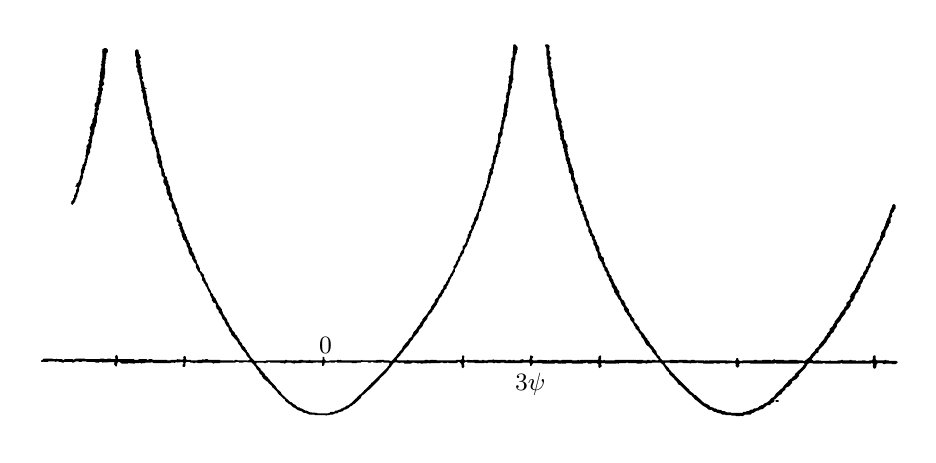
\begin{tikzpicture}[x=.2pt,y=-.2pt]
\path[use as bounding box] (0,0) rectangle (1590,735);
\path[fill=black,even odd rule]
(1351,674) -- (1352,676) -- (1357,676) -- (1357,674) -- (1356,673) -- (1352,673) -- cycle
(142,37) -- (139,37) -- (135,39) -- (135,43) -- (134,44) -- (135,45) -- (135,55) -- (134,56) -- (134,60) -- (133,61) -- (134,65) -- (132,67) -- (133,68) -- (133,73) -- (132,74) -- (132,79) -- (131,80) -- (131,85) -- (130,86) -- (130,88) -- (131,89) -- (131,93) -- (129,97) -- (130,98) -- (129,99) -- (130,101) -- (128,103) -- (129,105) -- (129,108) -- (127,109) -- (127,113) -- (128,114) -- (128,116) -- (127,117) -- (127,123) -- (125,125) -- (124,134) -- (121,138) -- (121,142) -- (123,144) -- (121,147) -- (121,153) -- (120,155) -- (122,156) -- (120,158) -- (120,161) -- (117,166) -- (117,172) -- (114,175) -- (114,178) -- (112,180) -- (114,188) -- (112,190) -- (113,192) -- (112,196) -- (111,197) -- (111,199) -- (112,200) -- (109,203) -- (110,205) -- (110,209) -- (106,214) -- (107,218) -- (106,219) -- (105,230) -- (104,231) -- (105,235) -- (103,238) -- (103,242) -- (102,243) -- (102,245) -- (99,248) -- (99,251) -- (96,258) -- (96,266) -- (94,270) -- (95,271) -- (94,272) -- (94,274) -- (92,277) -- (92,279) -- (88,282) -- (88,284) -- (86,287) -- (86,288) -- (88,287) -- (90,289) -- (90,290) -- (88,292) -- (87,298) -- (84,303) -- (84,307) -- (82,309) -- (82,311) -- (79,314) -- (79,316) -- (78,317) -- (80,320) -- (81,320) -- (86,314) -- (86,311) -- (88,309) -- (88,307) -- (90,305) -- (90,301) -- (93,294) -- (93,289) -- (97,281) -- (97,277) -- (100,271) -- (99,270) -- (100,269) -- (100,266) -- (99,265) -- (101,263) -- (102,261) -- (102,258) -- (104,256) -- (104,251) -- (106,248) -- (106,245) -- (107,244) -- (107,240) -- (108,239) -- (109,232) -- (113,225) -- (113,219) -- (115,216) -- (115,209) -- (116,208) -- (117,197) -- (120,191) -- (121,181) -- (123,178) -- (123,175) -- (125,171) -- (125,159) -- (127,157) -- (126,151) -- (129,147) -- (128,144) -- (129,143) -- (129,140) -- (132,135) -- (132,131) -- (133,130) -- (132,128) -- (132,125) -- (133,124) -- (133,121) -- (134,120) -- (134,115) -- (136,113) -- (136,110) -- (134,107) -- (138,103) -- (138,100) -- (136,96) -- (137,95) -- (137,93) -- (139,91) -- (139,85) -- (140,84) -- (140,73) -- (139,72) -- (140,68) -- (139,66) -- (141,64) -- (140,61) -- (141,60) -- (141,57) -- (142,56) -- (141,54) -- (142,52) -- (142,47) -- (145,44) -- (145,40) -- cycle
(1568,321) -- (1566,319) -- (1564,319) -- (1562,321) -- (1562,323) -- (1558,331) -- (1558,334) -- (1557,335) -- (1555,343) -- (1553,345) -- (1553,347) -- (1551,350) -- (1551,352) -- (1550,353) -- (1549,358) -- (1547,361) -- (1547,363) -- (1542,370) -- (1542,374) -- (1540,378) -- (1540,381) -- (1538,385) -- (1534,390) -- (1533,395) -- (1528,405) -- (1528,407) -- (1522,417) -- (1520,425) -- (1518,427) -- (1518,430) -- (1515,432) -- (1514,437) -- (1510,442) -- (1509,447) -- (1505,451) -- (1504,453) -- (1504,456) -- (1501,459) -- (1497,467) -- (1497,469) -- (1495,471) -- (1495,473) -- (1487,482) -- (1487,484) -- (1485,486) -- (1487,488) -- (1484,493) -- (1479,497) -- (1479,502) -- (1477,504) -- (1476,504) -- (1475,508) -- (1469,515) -- (1466,521) -- (1458,531) -- (1458,533) -- (1455,537) -- (1455,539) -- (1449,544) -- (1449,547) -- (1448,549) -- (1444,553) -- (1444,555) -- (1440,559) -- (1440,561) -- (1438,563) -- (1438,564) -- (1433,569) -- (1433,570) -- (1430,573) -- (1429,576) -- (1423,581) -- (1422,584) -- (1416,590) -- (1413,595) -- (1404,602) -- (1401,602) -- (1400,601) -- (1391,601) -- (1390,600) -- (1376,600) -- (1375,601) -- (1367,601) -- (1366,600) -- (1350,600) -- (1349,599) -- (1345,601) -- (1343,601) -- (1342,600) -- (1328,600) -- (1327,601) -- (1318,601) -- (1317,600) -- (1313,600) -- (1312,601) -- (1292,601) -- (1291,602) -- (1286,602) -- (1284,600) -- (1284,598) -- (1283,597) -- (1281,597) -- (1280,598) -- (1280,600) -- (1278,602) -- (1272,602) -- (1271,601) -- (1269,602) -- (1267,601) -- (1265,602) -- (1263,601) -- (1231,601) -- (1230,602) -- (1228,601) -- (1225,601) -- (1223,602) -- (1222,601) -- (1205,601) -- (1204,600) -- (1199,600) -- (1198,601) -- (1192,601) -- (1191,600) -- (1177,600) -- (1176,601) -- (1161,600) -- (1160,601) -- (1147,601) -- (1143,597) -- (1142,594) -- (1141,594) -- (1137,590) -- (1136,585) -- (1131,579) -- (1131,578) -- (1125,572) -- (1123,567) -- (1120,564) -- (1119,561) -- (1117,560) -- (1113,553) -- (1107,547) -- (1105,543) -- (1105,541) -- (1101,537) -- (1101,536) -- (1096,532) -- (1096,526) -- (1091,521) -- (1091,519) -- (1088,516) -- (1086,512) -- (1086,509) -- (1081,503) -- (1080,501) -- (1080,498) -- (1078,496) -- (1078,494) -- (1076,492) -- (1075,492) -- (1072,488) -- (1072,486) -- (1069,482) -- (1069,476) -- (1066,473) -- (1064,468) -- (1062,466) -- (1058,458) -- (1058,456) -- (1055,452) -- (1055,449) -- (1051,445) -- (1051,442) -- (1048,437) -- (1048,435) -- (1044,431) -- (1043,425) -- (1041,423) -- (1041,416) -- (1036,412) -- (1036,409) -- (1033,404) -- (1033,398) -- (1031,394) -- (1029,392) -- (1029,389) -- (1027,386) -- (1027,384) -- (1024,381) -- (1025,380) -- (1025,378) -- (1020,371) -- (1020,368) -- (1015,358) -- (1014,350) -- (1010,343) -- (1010,340) -- (1008,336) -- (1008,333) -- (1005,330) -- (1005,325) -- (1004,324) -- (1004,321) -- (1000,318) -- (1001,316) -- (1001,313) -- (998,310) -- (998,307) -- (994,298) -- (994,296) -- (995,295) -- (994,293) -- (995,291) -- (994,289) -- (994,285) -- (990,280) -- (989,273) -- (987,269) -- (987,263) -- (986,262) -- (987,260) -- (985,257) -- (985,255) -- (983,251) -- (983,248) -- (980,244) -- (981,243) -- (980,242) -- (980,237) -- (977,233) -- (977,231) -- (978,230) -- (976,227) -- (976,224) -- (975,223) -- (975,220) -- (976,219) -- (975,218) -- (975,216) -- (976,214) -- (975,213) -- (975,211) -- (973,209) -- (973,206) -- (969,201) -- (969,193) -- (968,192) -- (969,188) -- (968,187) -- (968,185) -- (966,183) -- (966,178) -- (964,175) -- (965,169) -- (964,168) -- (963,164) -- (961,162) -- (961,158) -- (960,157) -- (959,148) -- (955,139) -- (957,131) -- (954,125) -- (953,110) -- (951,108) -- (951,95) -- (948,90) -- (948,88) -- (949,87) -- (948,82) -- (949,80) -- (947,77) -- (947,74) -- (946,73) -- (946,70) -- (945,69) -- (945,66) -- (946,64) -- (944,62) -- (945,58) -- (946,57) -- (946,54) -- (943,51) -- (943,48) -- (944,47) -- (944,43) -- (942,41) -- (943,33) -- (940,30) -- (936,30) -- (935,31) -- (935,33) -- (937,37) -- (937,50) -- (938,51) -- (938,56) -- (939,57) -- (939,67) -- (940,68) -- (939,74) -- (941,76) -- (941,86) -- (943,90) -- (944,100) -- (945,101) -- (944,103) -- (944,106) -- (945,107) -- (945,112) -- (947,115) -- (947,122) -- (949,126) -- (949,131) -- (950,132) -- (950,137) -- (951,138) -- (952,147) -- (954,150) -- (954,160) -- (955,161) -- (955,165) -- (958,170) -- (958,178) -- (959,179) -- (959,184) -- (962,189) -- (961,191) -- (962,193) -- (962,196) -- (963,197) -- (962,201) -- (966,206) -- (965,208) -- (967,211) -- (967,216) -- (969,220) -- (969,224) -- (970,225) -- (970,228) -- (971,229) -- (971,232) -- (972,233) -- (972,238) -- (974,242) -- (974,245) -- (977,248) -- (976,249) -- (976,251) -- (977,252) -- (978,262) -- (980,263) -- (982,267) -- (982,274) -- (986,281) -- (986,285) -- (987,286) -- (987,291) -- (988,292) -- (988,295) -- (992,301) -- (992,308) -- (994,310) -- (994,314) -- (995,315) -- (996,319) -- (998,321) -- (998,325) -- (1000,328) -- (1000,331) -- (1002,332) -- (1002,336) -- (1004,339) -- (1004,341) -- (1006,343) -- (1006,347) -- (1008,350) -- (1010,359) -- (1011,359) -- (1013,362) -- (1013,368) -- (1016,373) -- (1016,376) -- (1017,376) -- (1019,378) -- (1020,383) -- (1022,386) -- (1022,391) -- (1025,395) -- (1027,403) -- (1029,405) -- (1031,416) -- (1033,418) -- (1034,421) -- (1037,424) -- (1037,426) -- (1039,428) -- (1039,431) -- (1042,435) -- (1042,438) -- (1046,443) -- (1046,447) -- (1050,452) -- (1050,456) -- (1052,458) -- (1055,464) -- (1055,467) -- (1059,473) -- (1060,479) -- (1062,480) -- (1062,482) -- (1065,485) -- (1068,491) -- (1070,492) -- (1073,500) -- (1077,505) -- (1077,508) -- (1080,514) -- (1082,515) -- (1083,518) -- (1088,524) -- (1089,528) -- (1094,534) -- (1096,539) -- (1098,541) -- (1098,543) -- (1104,549) -- (1104,551) -- (1108,555) -- (1109,559) -- (1112,562) -- (1117,572) -- (1120,575) -- (1121,575) -- (1128,583) -- (1128,585) -- (1136,594) -- (1136,595) -- (1140,599) -- (1140,600) -- (1139,601) -- (1134,601) -- (1133,600) -- (1129,600) -- (1128,601) -- (1124,601) -- (1123,600) -- (1120,600) -- (1119,601) -- (1112,601) -- (1111,600) -- (1105,600) -- (1104,601) -- (1103,600) -- (1101,600) -- (1100,601) -- (1098,600) -- (1062,600) -- (1061,601) -- (1043,601) -- (1041,600) -- (1040,601) -- (1037,601) -- (1035,599) -- (1036,598) -- (1036,593) -- (1034,592) -- (1031,595) -- (1031,599) -- (1030,600) -- (1005,600) -- (1004,601) -- (1003,600) -- (999,600) -- (998,601) -- (996,601) -- (995,600) -- (993,601) -- (984,601) -- (983,600) -- (965,600) -- (964,601) -- (959,601) -- (958,600) -- (947,600) -- (946,601) -- (942,601) -- (941,600) -- (940,601) -- (922,600) -- (921,601) -- (913,601) -- (911,599) -- (911,598) -- (913,596) -- (913,594) -- (909,592) -- (908,593) -- (907,599) -- (905,601) -- (904,600) -- (898,601) -- (894,599) -- (890,600) -- (889,601) -- (880,601) -- (879,600) -- (877,600) -- (876,601) -- (874,601) -- (873,600) -- (869,600) -- (868,601) -- (864,601) -- (863,600) -- (853,600) -- (851,601) -- (850,600) -- (842,600) -- (841,599) -- (840,600) -- (832,600) -- (831,601) -- (825,601) -- (824,600) -- (822,600) -- (821,601) -- (815,601) -- (814,600) -- (805,600) -- (804,601) -- (794,600) -- (793,601) -- (790,601) -- (788,599) -- (789,594) -- (787,592) -- (786,592) -- (785,593) -- (785,598) -- (783,600) -- (775,600) -- (774,601) -- (739,601) -- (738,600) -- (736,600) -- (735,601) -- (733,600) -- (727,600) -- (726,601) -- (724,601) -- (723,600) -- (718,600) -- (717,601) -- (688,601) -- (687,600) -- (686,601) -- (668,601) -- (667,600) -- (667,598) -- (674,591) -- (674,590) -- (678,586) -- (681,581) -- (688,574) -- (692,567) -- (696,563) -- (697,560) -- (706,550) -- (707,546) -- (713,540) -- (716,533) -- (722,526) -- (722,524) -- (724,520) -- (731,513) -- (731,511) -- (734,508) -- (734,507) -- (740,499) -- (740,497) -- (742,495) -- (742,493) -- (744,489) -- (749,484) -- (749,482) -- (752,478) -- (753,474) -- (757,471) -- (757,468) -- (760,464) -- (760,462) -- (762,460) -- (763,456) -- (766,450) -- (768,448) -- (770,443) -- (772,441) -- (772,436) -- (775,432) -- (778,426) -- (778,424) -- (780,422) -- (782,418) -- (782,415) -- (785,412) -- (785,410) -- (788,407) -- (789,401) -- (791,397) -- (793,395) -- (795,391) -- (795,388) -- (797,386) -- (797,383) -- (800,379) -- (800,377) -- (801,376) -- (801,372) -- (803,370) -- (803,368) -- (806,363) -- (806,361) -- (810,353) -- (810,351) -- (814,346) -- (816,333) -- (818,331) -- (819,331) -- (820,324) -- (823,318) -- (823,314) -- (825,311) -- (825,308) -- (828,303) -- (829,295) -- (831,292) -- (831,290) -- (833,288) -- (833,283) -- (835,280) -- (835,277) -- (836,276) -- (836,273) -- (837,272) -- (837,268) -- (839,266) -- (841,262) -- (840,257) -- (842,255) -- (843,247) -- (845,245) -- (846,235) -- (848,233) -- (848,229) -- (850,227) -- (851,217) -- (853,215) -- (853,213) -- (852,212) -- (855,208) -- (854,206) -- (854,200) -- (858,193) -- (858,184) -- (860,182) -- (860,175) -- (861,174) -- (861,171) -- (863,167) -- (863,163) -- (866,158) -- (866,152) -- (867,151) -- (866,147) -- (868,144) -- (870,123) -- (871,122) -- (871,119) -- (872,118) -- (872,113) -- (875,108) -- (874,102) -- (876,99) -- (876,96) -- (878,93) -- (877,91) -- (878,68) -- (879,67) -- (879,63) -- (880,62) -- (880,59) -- (881,58) -- (881,50) -- (883,48) -- (883,46) -- (884,45) -- (884,41) -- (885,40) -- (885,35) -- (881,30) -- (879,30) -- (877,32) -- (878,33) -- (877,35) -- (877,42) -- (876,43) -- (876,46) -- (877,48) -- (876,49) -- (876,53) -- (874,55) -- (874,60) -- (873,61) -- (873,64) -- (874,65) -- (873,66) -- (873,74) -- (872,75) -- (873,77) -- (872,79) -- (872,85) -- (869,88) -- (869,90) -- (870,91) -- (870,95) -- (869,96) -- (869,98) -- (870,100) -- (868,102) -- (868,111) -- (867,112) -- (867,116) -- (865,118) -- (865,122) -- (864,123) -- (864,126) -- (865,127) -- (865,129) -- (864,130) -- (864,134) -- (861,139) -- (861,146) -- (860,147) -- (860,153) -- (859,154) -- (859,161) -- (857,163) -- (858,166) -- (856,168) -- (856,175) -- (855,176) -- (855,179) -- (854,180) -- (853,188) -- (850,192) -- (850,203) -- (849,204) -- (849,208) -- (846,214) -- (846,220) -- (843,226) -- (843,230) -- (841,232) -- (841,238) -- (840,239) -- (840,244) -- (838,247) -- (838,252) -- (834,257) -- (835,260) -- (833,263) -- (833,266) -- (832,267) -- (832,271) -- (831,272) -- (831,276) -- (830,277) -- (830,282) -- (828,285) -- (828,288) -- (826,291) -- (826,294) -- (824,296) -- (824,298) -- (823,299) -- (823,303) -- (821,305) -- (821,310) -- (819,311) -- (818,313) -- (818,316) -- (816,320) -- (817,321) -- (815,324) -- (815,327) -- (814,328) -- (813,333) -- (811,336) -- (810,340) -- (807,344) -- (806,350) -- (804,353) -- (804,355) -- (801,359) -- (802,363) -- (797,369) -- (797,372) -- (795,374) -- (795,379) -- (793,381) -- (792,387) -- (790,391) -- (786,395) -- (786,401) -- (784,403) -- (781,409) -- (781,411) -- (778,414) -- (777,419) -- (774,423) -- (773,427) -- (769,432) -- (770,435) -- (766,443) -- (764,445) -- (763,449) -- (760,452) -- (759,456) -- (756,460) -- (756,462) -- (751,467) -- (751,470) -- (750,472) -- (747,475) -- (746,478) -- (742,483) -- (741,487) -- (737,490) -- (735,494) -- (736,495) -- (729,504) -- (728,508) -- (723,514) -- (722,517) -- (713,527) -- (713,529) -- (709,534) -- (708,537) -- (705,540) -- (702,545) -- (697,550) -- (696,554) -- (694,556) -- (694,558) -- (688,563) -- (688,565) -- (681,572) -- (681,573) -- (678,576) -- (676,581) -- (671,586) -- (671,587) -- (667,591) -- (667,592) -- (658,602) -- (654,602) -- (653,601) -- (644,601) -- (643,600) -- (635,600) -- (634,601) -- (632,600) -- (630,601) -- (605,601) -- (604,600) -- (602,601) -- (567,601) -- (566,600) -- (563,601) -- (562,600) -- (560,600) -- (559,601) -- (546,601) -- (545,602) -- (539,602) -- (536,599) -- (536,596) -- (535,595) -- (533,595) -- (533,600) -- (532,601) -- (511,601) -- (510,600) -- (508,601) -- (498,601) -- (497,600) -- (492,600) -- (491,601) -- (488,601) -- (487,602) -- (485,601) -- (480,601) -- (478,602) -- (477,601) -- (469,601) -- (468,600) -- (466,600) -- (465,601) -- (431,601) -- (430,602) -- (410,602) -- (403,595) -- (399,588) -- (396,585) -- (396,583) -- (394,581) -- (393,578) -- (388,574) -- (387,570) -- (383,566) -- (383,564) -- (379,559) -- (379,557) -- (375,554) -- (374,551) -- (370,547) -- (368,542) -- (366,540) -- (364,536) -- (364,534) -- (361,531) -- (361,529) -- (359,525) -- (356,522) -- (355,519) -- (353,517) -- (352,513) -- (351,512) -- (351,509) -- (344,500) -- (344,498) -- (342,496) -- (342,494) -- (340,492) -- (340,490) -- (335,484) -- (335,482) -- (331,478) -- (331,476) -- (327,469) -- (325,462) -- (323,460) -- (321,456) -- (321,454) -- (318,450) -- (319,449) -- (319,447) -- (315,443) -- (315,442) -- (311,439) -- (311,435) -- (308,428) -- (306,426) -- (305,420) -- (303,418) -- (303,414) -- (301,412) -- (301,410) -- (299,406) -- (297,404) -- (297,399) -- (293,394) -- (293,390) -- (291,388) -- (291,385) -- (288,382) -- (288,379) -- (286,376) -- (286,374) -- (284,372) -- (283,367) -- (281,364) -- (281,362) -- (279,358) -- (279,354) -- (274,347) -- (274,342) -- (273,341) -- (273,338) -- (272,337) -- (272,335) -- (270,333) -- (270,327) -- (268,326) -- (267,321) -- (263,313) -- (263,310) -- (261,307) -- (261,302) -- (260,301) -- (260,299) -- (258,297) -- (257,288) -- (254,282) -- (254,278) -- (252,275) -- (252,271) -- (251,269) -- (250,269) -- (248,267) -- (248,263) -- (246,260) -- (246,256) -- (244,253) -- (244,250) -- (243,249) -- (243,242) -- (241,239) -- (241,233) -- (238,227) -- (238,223) -- (237,222) -- (237,219) -- (235,216) -- (234,207) -- (233,206) -- (233,204) -- (231,202) -- (231,198) -- (229,195) -- (229,192) -- (228,191) -- (228,183) -- (225,180) -- (225,178) -- (224,177) -- (225,175) -- (225,169) -- (223,166) -- (223,163) -- (224,162) -- (222,158) -- (222,155) -- (219,151) -- (220,149) -- (220,145) -- (217,140) -- (217,136) -- (216,135) -- (217,134) -- (216,132) -- (216,124) -- (215,123) -- (215,120) -- (214,119) -- (214,115) -- (212,112) -- (213,110) -- (216,110) -- (215,109) -- (213,109) -- (211,107) -- (210,99) -- (206,94) -- (208,92) -- (208,89) -- (207,88) -- (207,82) -- (206,81) -- (206,74) -- (204,72) -- (205,68) -- (203,66) -- (204,61) -- (202,58) -- (202,57) -- (205,54) -- (203,51) -- (203,49) -- (201,47) -- (200,40) -- (197,39) -- (194,42) -- (194,51) -- (196,53) -- (196,64) -- (197,65) -- (196,71) -- (198,73) -- (198,79) -- (200,82) -- (200,85) -- (202,87) -- (202,93) -- (203,94) -- (204,102) -- (205,103) -- (205,108) -- (206,109) -- (206,112) -- (205,113) -- (208,119) -- (208,126) -- (210,130) -- (211,139) -- (213,142) -- (213,145) -- (214,146) -- (214,153) -- (215,154) -- (215,158) -- (217,160) -- (216,163) -- (220,171) -- (219,176) -- (221,179) -- (221,184) -- (223,186) -- (222,190) -- (225,197) -- (224,199) -- (224,204) -- (226,206) -- (227,209) -- (230,212) -- (230,217) -- (231,218) -- (232,224) -- (233,225) -- (233,234) -- (235,238) -- (235,244) -- (238,248) -- (237,249) -- (238,252) -- (241,255) -- (242,268) -- (243,268) -- (246,271) -- (246,274) -- (245,275) -- (245,280) -- (247,282) -- (247,284) -- (251,288) -- (250,289) -- (250,292) -- (251,293) -- (251,298) -- (252,299) -- (252,301) -- (256,306) -- (255,308) -- (255,311) -- (256,311) -- (260,316) -- (260,323) -- (261,324) -- (261,326) -- (263,328) -- (265,332) -- (265,335) -- (269,340) -- (269,342) -- (270,343) -- (269,349) -- (273,353) -- (272,357) -- (275,360) -- (274,363) -- (276,365) -- (276,368) -- (278,371) -- (278,375) -- (279,376) -- (279,378) -- (281,380) -- (281,383) -- (283,384) -- (287,391) -- (287,394) -- (290,399) -- (291,406) -- (293,410) -- (297,414) -- (297,418) -- (299,420) -- (300,423) -- (304,427) -- (304,433) -- (308,440) -- (312,444) -- (312,446) -- (315,451) -- (315,456) -- (318,459) -- (318,461) -- (321,464) -- (321,466) -- (323,468) -- (327,477) -- (329,479) -- (329,482) -- (333,490) -- (333,493) -- (336,497) -- (338,497) -- (340,499) -- (340,504) -- (341,505) -- (341,507) -- (345,511) -- (345,514) -- (350,520) -- (352,526) -- (356,530) -- (356,532) -- (359,538) -- (363,542) -- (363,545) -- (365,549) -- (367,551) -- (368,555) -- (379,567) -- (381,572) -- (384,575) -- (387,581) -- (394,588) -- (396,593) -- (401,598) -- (401,600) -- (397,602) -- (396,601) -- (379,601) -- (378,600) -- (376,600) -- (372,602) -- (371,601) -- (348,601) -- (347,600) -- (326,600) -- (325,599) -- (321,599) -- (320,600) -- (316,599) -- (315,600) -- (308,600) -- (307,601) -- (295,601) -- (294,600) -- (289,600) -- (288,601) -- (286,599) -- (286,595) -- (284,593) -- (282,594) -- (281,596) -- (282,598) -- (280,600) -- (270,599) -- (269,600) -- (259,600) -- (258,601) -- (252,601) -- (251,600) -- (226,600) -- (225,599) -- (219,599) -- (218,600) -- (216,600) -- (215,599) -- (201,599) -- (200,600) -- (193,600) -- (192,599) -- (164,599) -- (163,598) -- (163,595) -- (161,591) -- (160,591) -- (158,594) -- (158,596) -- (159,597) -- (158,599) -- (151,599) -- (150,598) -- (144,598) -- (143,599) -- (139,599) -- (138,598) -- (131,598) -- (130,599) -- (104,599) -- (103,598) -- (87,598) -- (83,600) -- (81,599) -- (67,599) -- (66,600) -- (63,600) -- (62,599) -- (53,599) -- (52,598) -- (50,599) -- (46,599) -- (45,598) -- (29,598) -- (27,600) -- (26,600) -- (24,602) -- (24,603) -- (25,604) -- (28,604) -- (29,603) -- (30,604) -- (36,604) -- (37,603) -- (49,603) -- (51,604) -- (52,603) -- (56,603) -- (57,604) -- (61,604) -- (62,605) -- (65,605) -- (66,604) -- (80,604) -- (81,605) -- (83,605) -- (87,603) -- (92,603) -- (93,604) -- (97,604) -- (98,603) -- (106,603) -- (107,604) -- (122,604) -- (123,605) -- (129,605) -- (130,604) -- (134,604) -- (135,605) -- (156,604) -- (157,605) -- (156,608) -- (159,612) -- (161,612) -- (162,606) -- (164,604) -- (166,604) -- (170,607) -- (181,607) -- (182,606) -- (193,607) -- (194,606) -- (201,606) -- (202,605) -- (206,607) -- (207,606) -- (212,606) -- (213,605) -- (223,605) -- (224,604) -- (228,606) -- (258,606) -- (259,605) -- (264,605) -- (266,606) -- (268,604) -- (270,605) -- (280,604) -- (282,606) -- (280,609) -- (280,612) -- (281,613) -- (283,613) -- (285,611) -- (285,606) -- (287,604) -- (293,604) -- (294,605) -- (298,605) -- (299,606) -- (302,606) -- (303,605) -- (306,605) -- (307,606) -- (315,606) -- (316,605) -- (332,605) -- (336,607) -- (337,606) -- (347,606) -- (348,605) -- (375,605) -- (376,604) -- (381,604) -- (382,605) -- (389,605) -- (390,604) -- (405,605) -- (412,613) -- (414,617) -- (418,621) -- (419,625) -- (423,628) -- (423,630) -- (425,632) -- (425,633) -- (432,639) -- (433,639) -- (435,641) -- (435,642) -- (441,647) -- (443,651) -- (444,651) -- (451,658) -- (451,659) -- (455,664) -- (456,664) -- (463,671) -- (465,672) -- (465,674) -- (468,677) -- (469,677) -- (472,680) -- (475,681) -- (480,686) -- (483,687) -- (488,691) -- (495,693) -- (499,696) -- (502,696) -- (509,699) -- (518,699) -- (519,700) -- (538,700) -- (539,701) -- (541,700) -- (545,700) -- (546,699) -- (551,699) -- (555,697) -- (559,697) -- (561,695) -- (569,693) -- (572,690) -- (574,690) -- (580,687) -- (583,684) -- (586,683) -- (589,680) -- (590,680) -- (602,669) -- (603,666) -- (606,663) -- (607,663) -- (615,655) -- (616,655) -- (636,635) -- (636,634) -- (648,623) -- (648,622) -- (652,618) -- (652,617) -- (657,612) -- (658,609) -- (660,608) -- (660,607) -- (662,605) -- (664,605) -- (665,604) -- (667,605) -- (670,605) -- (671,606) -- (673,606) -- (674,605) -- (679,605) -- (681,607) -- (692,607) -- (696,605) -- (704,606) -- (705,607) -- (707,606) -- (709,606) -- (710,607) -- (726,606) -- (727,607) -- (728,606) -- (745,606) -- (746,605) -- (750,605) -- (751,606) -- (757,606) -- (758,605) -- (760,605) -- (761,606) -- (775,606) -- (778,604) -- (780,604) -- (783,607) -- (784,609) -- (784,613) -- (786,615) -- (787,615) -- (789,612) -- (788,606) -- (791,604) -- (794,604) -- (795,605) -- (807,605) -- (808,606) -- (825,606) -- (826,605) -- (828,606) -- (831,606) -- (832,605) -- (840,605) -- (841,606) -- (844,606) -- (845,605) -- (847,605) -- (848,606) -- (854,606) -- (855,605) -- (861,605) -- (862,606) -- (893,606) -- (894,605) -- (906,605) -- (908,608) -- (908,611) -- (910,611) -- (913,606) -- (929,606) -- (930,607) -- (952,607) -- (953,606) -- (957,606) -- (958,607) -- (964,607) -- (965,606) -- (966,607) -- (972,607) -- (973,606) -- (983,606) -- (984,607) -- (1003,607) -- (1004,606) -- (1008,606) -- (1009,605) -- (1011,605) -- (1013,607) -- (1018,607) -- (1019,606) -- (1028,606) -- (1031,608) -- (1031,613) -- (1033,615) -- (1037,612) -- (1037,610) -- (1036,609) -- (1036,607) -- (1037,606) -- (1043,606) -- (1044,607) -- (1063,607) -- (1065,606) -- (1066,607) -- (1068,607) -- (1069,606) -- (1081,606) -- (1082,605) -- (1084,605) -- (1085,606) -- (1100,606) -- (1101,607) -- (1109,607) -- (1110,606) -- (1116,606) -- (1117,607) -- (1119,607) -- (1120,606) -- (1127,606) -- (1128,605) -- (1143,605) -- (1148,609) -- (1155,620) -- (1159,623) -- (1159,626) -- (1168,634) -- (1168,635) -- (1173,640) -- (1176,645) -- (1179,646) -- (1195,662) -- (1199,664) -- (1207,673) -- (1208,673) -- (1220,683) -- (1227,687) -- (1230,690) -- (1232,690) -- (1233,691) -- (1235,690) -- (1240,694) -- (1243,694) -- (1246,696) -- (1252,697) -- (1255,699) -- (1260,699) -- (1261,700) -- (1271,700) -- (1272,701) -- (1279,701) -- (1280,702) -- (1287,702) -- (1288,701) -- (1292,702) -- (1296,699) -- (1306,699) -- (1309,696) -- (1311,696) -- (1317,692) -- (1320,692) -- (1323,690) -- (1328,689) -- (1336,682) -- (1341,682) -- (1344,678) -- (1347,677) -- (1349,675) -- (1349,672) -- (1350,671) -- (1351,671) -- (1358,664) -- (1362,662) -- (1364,658) -- (1369,654) -- (1369,652) -- (1372,649) -- (1374,649) -- (1378,646) -- (1378,645) -- (1381,642) -- (1381,639) -- (1390,634) -- (1390,633) -- (1394,629) -- (1394,626) -- (1405,615) -- (1409,608) -- (1412,606) -- (1418,606) -- (1419,607) -- (1436,607) -- (1437,606) -- (1440,606) -- (1441,607) -- (1468,607) -- (1469,606) -- (1471,606) -- (1472,607) -- (1523,607) -- (1524,606) -- (1526,606) -- (1528,608) -- (1527,610) -- (1527,613) -- (1529,616) -- (1531,616) -- (1533,614) -- (1534,608) -- (1536,606) -- (1544,606) -- (1547,608) -- (1549,608) -- (1550,607) -- (1561,607) -- (1562,608) -- (1568,608) -- (1572,605) -- (1572,604) -- (1569,602) -- (1556,602) -- (1555,601) -- (1551,601) -- (1550,600) -- (1548,601) -- (1534,601) -- (1532,599) -- (1532,593) -- (1531,592) -- (1529,592) -- (1527,594) -- (1527,599) -- (1525,601) -- (1521,601) -- (1520,602) -- (1514,602) -- (1513,601) -- (1497,602) -- (1496,601) -- (1489,601) -- (1488,600) -- (1486,600) -- (1485,601) -- (1473,601) -- (1472,600) -- (1470,600) -- (1469,601) -- (1464,601) -- (1463,602) -- (1451,602) -- (1450,601) -- (1448,602) -- (1433,602) -- (1432,601) -- (1430,602) -- (1429,601) -- (1424,601) -- (1423,602) -- (1420,602) -- (1416,599) -- (1419,596) -- (1419,595) -- (1422,592) -- (1423,592) -- (1423,590) -- (1425,588) -- (1427,588) -- (1429,586) -- (1429,583) -- (1439,573) -- (1439,572) -- (1443,568) -- (1446,562) -- (1450,558) -- (1451,554) -- (1456,550) -- (1458,545) -- (1462,540) -- (1462,537) -- (1463,535) -- (1468,530) -- (1471,524) -- (1477,517) -- (1478,515) -- (1478,512) -- (1481,509) -- (1482,509) -- (1487,502) -- (1487,498) -- (1488,496) -- (1492,493) -- (1492,491) -- (1494,489) -- (1494,486) -- (1495,485) -- (1496,481) -- (1501,477) -- (1501,474) -- (1504,471) -- (1504,469) -- (1505,468) -- (1505,464) -- (1507,462) -- (1509,458) -- (1509,456) -- (1512,453) -- (1514,449) -- (1514,447) -- (1517,444) -- (1517,442) -- (1519,440) -- (1519,438) -- (1521,434) -- (1523,432) -- (1523,426) -- (1528,420) -- (1528,417) -- (1534,407) -- (1534,404) -- (1538,400) -- (1538,396) -- (1542,390) -- (1542,387) -- (1545,383) -- (1545,381) -- (1549,377) -- (1549,374) -- (1550,373) -- (1549,371) -- (1550,370) -- (1550,368) -- (1556,358) -- (1556,355) -- (1558,353) -- (1559,353) -- (1559,344) -- (1562,341) -- (1562,339) -- (1561,338) -- (1562,335) -- (1565,332) -- (1566,329) -- (1568,327) -- cycle
(1151,606) -- (1152,605) -- (1160,605) -- (1161,606) -- (1175,606) -- (1176,605) -- (1183,605) -- (1184,606) -- (1196,606) -- (1197,607) -- (1198,606) -- (1208,606) -- (1209,605) -- (1211,605) -- (1212,606) -- (1220,606) -- (1221,607) -- (1239,607) -- (1240,606) -- (1244,606) -- (1245,607) -- (1250,607) -- (1251,606) -- (1260,606) -- (1261,607) -- (1264,607) -- (1266,606) -- (1267,607) -- (1268,606) -- (1278,606) -- (1280,608) -- (1279,609) -- (1279,611) -- (1282,614) -- (1283,614) -- (1286,611) -- (1285,608) -- (1288,606) -- (1290,606) -- (1291,607) -- (1292,606) -- (1305,606) -- (1306,607) -- (1349,607) -- (1350,606) -- (1352,606) -- (1353,607) -- (1361,607) -- (1362,606) -- (1363,607) -- (1393,607) -- (1394,606) -- (1402,606) -- (1404,608) -- (1401,611) -- (1401,612) -- (1386,626) -- (1386,628) -- (1384,630) -- (1383,630) -- (1380,634) -- (1379,634) -- (1374,638) -- (1374,639) -- (1367,646) -- (1363,652) -- (1361,652) -- (1360,654) -- (1352,661) -- (1349,666) -- (1347,668) -- (1344,669) -- (1341,672) -- (1341,673) -- (1336,677) -- (1331,679) -- (1328,682) -- (1326,682) -- (1322,684) -- (1319,687) -- (1317,687) -- (1316,688) -- (1312,688) -- (1310,690) -- (1307,690) -- (1302,693) -- (1299,693) -- (1298,694) -- (1293,694) -- (1292,696) -- (1271,696) -- (1270,695) -- (1263,695) -- (1259,693) -- (1255,693) -- (1253,691) -- (1246,690) -- (1243,688) -- (1240,688) -- (1238,686) -- (1236,686) -- (1235,685) -- (1234,686) -- (1231,682) -- (1225,679) -- (1223,679) -- (1207,664) -- (1204,663) -- (1202,660) -- (1201,660) -- (1196,656) -- (1195,653) -- (1193,652) -- (1169,628) -- (1169,627) -- (1163,622) -- (1163,621) -- (1159,617) -- (1159,616) -- (1153,610) -- cycle
(413,609) -- (413,606) -- (414,605) -- (426,605) -- (427,606) -- (430,606) -- (431,605) -- (434,605) -- (435,604) -- (437,604) -- (438,605) -- (456,605) -- (457,606) -- (463,606) -- (464,607) -- (468,605) -- (476,605) -- (477,606) -- (482,607) -- (483,606) -- (494,606) -- (495,605) -- (515,606) -- (516,605) -- (521,605) -- (523,604) -- (524,605) -- (531,605) -- (532,606) -- (532,611) -- (534,611) -- (536,609) -- (536,607) -- (538,605) -- (545,605) -- (546,604) -- (548,605) -- (555,605) -- (556,604) -- (558,604) -- (559,605) -- (585,605) -- (586,606) -- (594,606) -- (595,605) -- (602,605) -- (603,604) -- (614,604) -- (615,605) -- (620,605) -- (621,604) -- (624,604) -- (625,605) -- (630,605) -- (631,606) -- (632,605) -- (639,605) -- (640,604) -- (642,604) -- (643,605) -- (652,605) -- (654,607) -- (653,608) -- (653,610) -- (650,613) -- (650,614) -- (623,641) -- (622,641) -- (620,643) -- (620,644) -- (618,646) -- (617,646) -- (616,648) -- (609,655) -- (608,655) -- (607,657) -- (601,663) -- (600,663) -- (596,667) -- (595,667) -- (595,669) -- (593,670) -- (584,679) -- (583,679) -- (580,682) -- (576,683) -- (573,686) -- (571,686) -- (569,688) -- (567,688) -- (565,690) -- (563,690) -- (559,692) -- (556,692) -- (554,694) -- (547,694) -- (546,696) -- (544,696) -- (543,697) -- (524,697) -- (523,696) -- (510,695) -- (504,692) -- (502,692) -- (495,688) -- (493,688) -- (491,686) -- (488,686) -- (483,681) -- (480,680) -- (477,677) -- (474,676) -- (459,662) -- (457,658) -- (451,653) -- (448,648) -- (438,638) -- (438,637) -- (434,633) -- (434,632) -- (429,628) -- (428,625) -- (424,621) -- (424,620) -- (423,620) -- (421,618) -- (421,616) -- (419,615) -- cycle;
\node[inner sep=0,font=\fontsize{9}{11}\selectfont] at (538,574) {$0$};
\node[inner sep=0,font=\fontsize{9}{11}\selectfont] at (908,644) {$3\psi$};
\end{tikzpicture}
\end{center}

\noindent $y$ gives the abscissas and $\boldsymbol{P}y$ the ordinates.

We denote the value of $\Pi z$ at $z=0$ by $\psi$ (approximately
$=1{,}402186$). Then $6\psi$ is the length of the period in general, i.\,e.
$\boldsymbol{P}\varphi=\boldsymbol{P}(\varphi+6k\psi)$, where $k$ denotes any
integer.

\clearpage
\SourceLeaf{101}%

\[
\boldsymbol{P}(0)=-1,\qquad \boldsymbol{P}\varphi=\boldsymbol{P}(-\varphi),\qquad
\boldsymbol{P}\psi=0,\qquad \boldsymbol{P}(2\varphi)=2,\qquad \boldsymbol{P}(3\psi)=\infty,
\]
\[
\boldsymbol{P}(\varphi+3\psi)=\frac{2-\boldsymbol{P}(\varphi)}{1+\boldsymbol{P}(\varphi)},
\qquad \boldsymbol{P}(1\tfrac12\psi)=\sqrt{3}-1.
\]

\noindent If
\[
\boldsymbol{P}\varphi=s,\qquad \boldsymbol{P}(\varphi+2\psi)=c,
\]
\noindent then
\[
s\,s\,c\,c=4s+4c,\qquad c=\frac{2(1+\sqrt{1+s^3})}{s\,s},
\]
\[
\boldsymbol{P}(3\psi+\varphi+\varphi')=
\frac{2+s s'(s+s')-\tfrac12(c s s-2)(c' s' s'-2)}{(s-s')^2},
\]
\[
\boldsymbol{P}(3\psi+\varphi-\varphi')=
\frac{2+s s'(s+s')+\tfrac12(c s s-2)(c' s' s'-2)}{(s-s')^2}.
\]



\Needspace{10\baselineskip}
The preceding statements hold for the indicated meaning of our terms. If, however, we let
$\Pi z$ denote the value of the integral $\int \frac{dx}{\BareRoot{(1+x^3)}}$ from $x=-1$ to $x=z-1$
(which may be illustrated by shifting the axis of abscissas down by 1),
we obtain

\[
\boldsymbol{P}(0)=0,\quad \boldsymbol{P}\psi=1,\quad \boldsymbol{P}(2\psi)=3,\quad
\boldsymbol{P}(3\psi)=\infty,\quad \boldsymbol{P}(3\psi-\varphi)=\frac{3}{\boldsymbol{P}(\psi)},
\]
\[
\boldsymbol{P}(2\varphi)=
\frac{12\boldsymbol{P}\varphi\left(\boldsymbol{P}(\varphi)^2-3\boldsymbol{P}\varphi+3\right)}
{\left(\boldsymbol{P}(\varphi)^2-3\right)^2},
\]
\[
\boldsymbol{P}(\varphi+\varphi')=
\frac{\begin{gathered}3(s+s')s s'-18 s s'+9(s+s')\\{}+6\sqrt{(s^3-3ss+3s)(s'^3-3s's'+3s')}\end{gathered}}{(ss'-3)^2}.
\]



\Needspace{5\baselineskip}
\[
\Pi(1+z)=\psi+z-\frac14\cdot\frac12 z^4+\frac17\cdot\frac{1.3}{2.4}z^7
-\frac{1}{10}\cdot\frac{1.3.5}{2.4.6}z^{10}+\cdots,
\]
\[
\Pi(1+z)=3\psi-2\sqrt{z}\left(\frac1z-\frac17\cdot\frac12\frac{1}{z^4}
+\frac{1}{13}\cdot\frac{1.3}{2.4}\cdot\frac{1}{z^7}-\cdots\right),
\]
\[
\psi=1{,}4021822
\]
\[
\log\psi=0{,}1468045
\]
\[
\log\mathrm{hyp}\,\psi=0{,}3380399.
\]



\Needspace{14\baselineskip}
\SourceLeaf{102}%
\begin{center}
REMARKS ON THE INVESTIGATIONS INTO THE FUNCTIONS ARISING FROM THE INTEGRAL
$\displaystyle\int\frac{dx}{\BareRoot{(1+x^3)}}$.
\end{center}

\noindent\hspace*{\parindent}According to a diary entry, \textsc{Gauss} inverted the integral considered here
into the concluding power series as early as 9\ September 1796.

The approach developed here bears a relation to \textsc{Weierstrass}’s theory corresponding to
that of the investigation of the lemniscatic integral to \textsc{Jacobi}’s theory.
The latter integral gives the so-called »harmonic« case of the elliptic
structure, while the case here is the »equianharmonic« one.

All of \textsc{Gauss}’s statements follow readily from the addition theorem
for $\boldsymbol{P}(\varphi)$, i.\,e. from the formula given above for
$\boldsymbol{P}(3\psi+\varphi+\varphi')$, which, written somewhat differently, takes the form
\[
\boldsymbol{P}(3\psi+\varphi+\varphi')=
\frac{\begin{gathered}\boldsymbol{P}(\varphi)\boldsymbol{P}(\varphi')
(\boldsymbol{P}(\varphi)+\boldsymbol{P}(\varphi'))\\{}
+2-2\sqrt{1+\boldsymbol{P}(\varphi)^3}\sqrt{1+\boldsymbol{P}(\varphi')^3}\end{gathered}}
{(\boldsymbol{P}(\varphi)-\boldsymbol{P}(\varphi'))^2},
\]
\noindent and which \textsc{Gauss} undoubtedly obtained by the method he also followed for the
lemniscatic integral, i.\,e. through \textsc{Euler}’s original line of reasoning.
Incidentally, this formula reduces directly to the addition theorem for
\textsc{Weierstrass}’s function $\wp(u)$ with $g_2=0$, $g_3=-4$.

\Needspace{12\baselineskip}
The addition theorem readily gives the following formulas.
\[
\boldsymbol{P}(2\varphi+3\psi)=\frac{\boldsymbol{P}(\varphi)(\boldsymbol{P}(\varphi)^3-8)}
{4(\boldsymbol{P}(\varphi)^3+1)},
\]
\[
\boldsymbol{P}(3\varphi)=\frac{\boldsymbol{P}(\varphi)^9-96\boldsymbol{P}(\varphi)^6+48\boldsymbol{P}(\varphi)^3+64}
{9\boldsymbol{P}(\varphi)^2(\boldsymbol{P}(\varphi)^3+4)^2}.
\]
\noindent Using these equations and starting from $\boldsymbol{P}(0)=-1$,
$\boldsymbol{P}(\psi)=0$, one readily derives the remaining statements of \textsc{Gauss}.\hfill\textsc{Fricke.}

\clearpage
\SourceLeaf{103}%

\begin{center}
\large [INVERSION OF THE ELLIPTIC INTEGRAL OF THE FIRST KIND.]
\end{center}

\bigskip

\noindent\hspace*{\parindent}On the transcendental function $\displaystyle\int\frac{dx}{\BareRoot{(1-xx)(1-\mu xx)}}=\varphi$, where we put \mbox{$x=f\varphi$}.

Putting $\log x = y$, we have

\[ \frac{x\,dy}{d\varphi} = \BareRoot{(1-xx)(1-\mu xx)}, \]

\[ \frac{ddy}{d\varphi^2} = -\frac{dx}{x\,d\varphi}\cdot\frac{dy}{d\varphi} - \frac{x\,dx}{(1-xx)\,d\varphi}\cdot\frac{dy}{d\varphi} - \frac{\mu x\,dx}{(1-\mu xx)\,d\varphi}\cdot\frac{dy}{d\varphi}, \]

\[ \frac{ddy}{d\varphi^2} = -\frac{(1-xx)(1-\mu xx)}{xx} - (1-\mu xx) - \mu(1-xx), \]

\[ \frac{ddy}{d\varphi^2} = -\frac{1}{xx} + \mu xx. \]

\noindent Let

\[ \int\frac{d\varphi}{xx} = t, \qquad \int \mu xx\,d\varphi = u, \]

\noindent then we shall have

\[ \frac{dy}{d\varphi} = u - t. \]

\noindent Further, let

\[ \int u\,d\varphi = v, \qquad \int t\,d\varphi = w, \]

\noindent then we shall have

\[ y = v - w. \]

\noindent We shall put

\[ e^{-w} = P\varphi, \qquad e^{-v} = Q\varphi, \]

\[ PP'' = P'P' - QQ, \qquad QQ'' = Q'Q' - \mu PP. \]

\[ P = \varphi - \tfrac{1}{6}(1+\mu)\varphi^3 + \tfrac{1}{120}(1+4\mu+\mu\mu)\varphi^5 - \cdots, \]

\[\begin{aligned} Q &= 1+\ast-\tfrac{1}{12}\mu\varphi^4+\tfrac{1}{90}(\mu+\mu\mu)\varphi^6\\&\quad-\tfrac{1}{10080}(8\mu+17\mu\mu+8\mu^3)\varphi^8-\cdots.\end{aligned}\]

\bigskip


\Needspace{16\baselineskip}
\SourceLeaf{104}%

\begin{center}
REMARKS ON THE INVERSION OF THE ELLIPTIC INTEGRAL OF THE FIRST KIND.
\end{center}

\noindent\hspace*{\parindent}This note, probably datable from the diary entry of 6\ May 1800, »Theoriam quantitatum transcendentium $\int\frac{dx}{\BareRoot{(1-a xx)(1-\beta xx)}}$ ad summam universalitatem perduximus«, is among the most interesting derivations that \textsc{Gauss} carried out in the field of elliptic functions. In its formulation of the problem and its notation, it follows the investigations »Elegantiores integralis $\int\frac{dx}{\BareRoot{(1-x^4)}}$ proprietates« (ges. Werke III p.\,404 ff.), which belong to the earliest period of his work on lemniscatic functions. On the other hand, in 1799 \textsc{Gauss} studied the inversion of the general integral of the first kind $\int\frac{du}{\BareRoot{(1+\mu\mu\sin u^2)}}$.

The letter from \textsc{Gauss} to \textsc{Bessel} printed above sheds particularly interesting light on the mathematics developed here. In it \textsc{Gauss} repeatedly emphasizes the importance of entire transcendental functions. In an elegant derivation, the function $f\varphi$, which \textsc{Jacobi} later denoted by $\sin\mathrm{am}\,\varphi$, is here represented as the quotient of two functions $P\varphi$ and $Q\varphi$, which \textsc{Gauss} unquestionably knew to be \textls{entire} transcendental functions.

It may also be noted that the functions $P, Q$ that \textsc{Gauss} introduces here are precisely those to which \textsc{Weierstrass}, building on the work of \textsc{Abel}, later gave the designations $\mathrm{Al}(\varphi)_1$ and $\mathrm{Al}(\varphi)_0$.

\hfill \textsc{Fricke}.

\bigskip


\clearpage
\SourceLeaf{105}%

\begin{center}
\large A MOST ELEGANT THEOREM.
\end{center}

\bigskip

\noindent\hspace*{\parindent}Let

\[ 1+\tfrac{1}{2}\cdot\tfrac{1}{2}xx+\tfrac{1}{2}\cdot\tfrac{1}{2}\cdot\tfrac{3}{4}\cdot\tfrac{3}{4}x^4+\tfrac{1}{2}\cdot\tfrac{1}{2}\cdot\tfrac{3}{4}\cdot\tfrac{3}{4}\cdot\tfrac{5}{6}\cdot\tfrac{5}{6}x^6+\text{etc.} = fx, \]

\[ \tfrac{1}{2}x+\tfrac{1}{2}\cdot\tfrac{3}{2}\cdot\tfrac{3}{4}x^3+\tfrac{1}{2}\cdot\tfrac{3}{2}\cdot\tfrac{3}{4}\cdot\tfrac{5}{4}\cdot\tfrac{5}{6}x^5+\text{etc.} = f'x, \]

\noindent then we shall have

\[ \sin\varphi\, f\sin\varphi\, f'\cos\varphi + \cos\varphi\, f\cos\varphi\, f'\sin\varphi = \frac{2}{\pi\sin\varphi\cos\varphi}. \]

\bigskip

\bigskip

\begin{center}
REMARKS ON »THEOREMA ELEGANTISSIMUM«.
\end{center}

\noindent\hspace*{\parindent}\textsc{Gauss} wrote this theorem on the last page of his own copy of »\textsc{Euler}, Methodus inveniendi curvas Maximi Minimive proprietate gaudentes«. The theorem was included here because of the elegant form of the concluding formula, which evidently struck \textsc{Gauss} himself. In substance, this is one of the simplest differential relations in the theory of the arithmetic-geometric mean, as can be shown with the aid of a few formulas from Art.\,13 and 14 of »Arithmetisch-geometrischen Mittels« (cf. ges. Werke III p.\,379 ff.). For $fx$ proves to be the \textsc{Gauss}ian series $F(\tfrac{1}{2},\tfrac{1}{2},1;x^2)$, so that, using the last two formulas on p.\,381 l.\,c., we may put:

\[ x=\sin\varphi=\frac{b}{a}, \qquad \sqrt{1-x^2}=\cos\varphi=\frac{c}{a}, \]

\[ f\sin\varphi=\frac{a}{M( a,c)}, \qquad f\cos\varphi=\frac{a}{M( a,b)}. \]

\noindent After a simple intermediate calculation, the theorem stated here then takes the form:

\[ \frac{b^2\mathord{.} d\log\dfrac{a}{M( a,b)}}{d\log\dfrac{c}{a}} - \frac{c^2\mathord{.} d\log\dfrac{a}{M( a,c)}}{d\log\dfrac{a}{b}} = \frac{2}{\pi}\,M( a,b)\,M( a,c), \]

\noindent a formula that is a simple consequence of the first equations on p.\,380 l.\,c.

\hfill \textsc{Fricke}.

\bigskip


\end{document}
